\documentclass[a4paper]{article}
\usepackage[english]{babel}
\usepackage[utf8x]{inputenc}
\usepackage[T1]{fontenc}
\usepackage{float}
%% Sets page size and margins
\usepackage[a4paper,top=3cm,bottom=2cm,left=3cm,right=3cm,marginparwidth=1.75cm]{geometry}

%% Useful packages
\usepackage{pgf,tikz,pgfplots}
\pgfplotsset{compat=1.15}
\usepackage{mathrsfs}
\usepackage{fancyhdr}
\pagestyle{fancy}
\usepackage{amsmath}
\usepackage{amstext}
\usepackage{amsthm}
\usepackage{enumitem}
\usepackage{eqnarray}
\usepackage{float}
\usepackage{esint}
\usepackage{wrapfig}
\usepackage{gensymb}
\usepackage{lipsum}
\usepackage{amssymb}
\usepackage{array}
\usepackage{tikz}
\usepackage[colorlinks=true, allcolors=blue]{hyperref}
\usepackage{graphicx}
\usepackage{amsmath}
\usepackage{amssymb}

\usepackage{graphicx}
\usepackage{mathtools}


%declare math operators
\DeclareMathOperator{\ccl}{ccl}
\DeclareMathOperator{\ord}{ord}
\DeclareMathOperator{\SL}{SL}
\DeclareMathOperator{\GL}{GL}
\DeclareMathOperator{\Id}{Id}
\DeclareMathOperator{\res}{res}
\DeclareMathOperator{\cosech}{cosech}
\DeclareMathOperator{\cosec}{cosec}
\DeclareMathOperator{\im}{Im}
\DeclareMathOperator{\Span}{Span}
\DeclareMathOperator{\Sym}{Sym}
\DeclareMathOperator{\Auto}{Aut}
\DeclareMathOperator{\lcm}{lcm}
\DeclareMathOperator{\Tr}{Tr}
\DeclareMathOperator{\tr}{Tr}
\DeclareMathOperator{\erf}{erf}
\DeclareMathOperator{\erfc}{erfc}
\DeclareMathOperator{\sech}{sech}
\DeclareMathOperator{\Ker}{Ker}
\DeclareMathOperator{\diag}{diag}
\DeclareMathOperator{\sgn}{sgn}
\DeclareMathOperator{\Mod}{mod}
\DeclareMathOperator{\cl}{cl}
\newcommand{\iso}{\xrightarrow{
   \,\smash{\raisebox{-0.65ex}{\ensuremath{\scriptstyle\sim}}}\,}}
   
   
%environment
\newtheorem*{notation*}{Notation}
\newtheorem*{foreword*}{Foreword}
\newtheorem{eg}{Example}[section]
\newtheorem{remarks}{Remarks}[section]
\newtheorem{notation}{Notation}[section]
\definecolor{darkblue}{RGB}{	0, 0, 139}
\newtheoremstyle{new}% <name>
{2pt}% <Space above>
{2pt}% <Space below>
{\color{darkblue}}% Body font
{}% <Indent amount>
{\bfseries\color{black}}% Theorem head font
{:}% <Punctuation after theorem head>
{.5em}% <Space after theorem headi>
{}% <Theorem head spec (can be left empty, meaning `normal')>
\theoremstyle{new}

\newtheorem{defi}{Definition}[section]
\newtheorem{thm}{Theorem}[section]
\newtheorem{prop}{Proposition}[section]
\newtheorem{lemma}{Lemma}[section]
\newtheorem{cor}{Corollary}[section]

\title{\textbf{NST Mathematics Part IB Summary Notes}}
\author{Tai Yingzhe, Tommy (ytt26)}
\date{}
\setlength{\parindent}{0cm}
\begin{document}
\maketitle
\usetikzlibrary{decorations.markings}
\tikzset{->-/.style={decoration={
  markings,
  mark=at position #1 with {\arrow{>}}},postaction={decorate}}}
\tikzset{-<-/.style={decoration={
  markings,
  mark=at position #1 with {\arrow{<}}},postaction={decorate}}}
{\small\tableofcontents}
\begin{notation*}
b.c.s stands for boundary conditions, i.c.s stands for initial conditions, s.t. stands for such that.
\end{notation*}
\begin{foreword*}
A notes compilation for IB Mathematics for the Natural Science Tripos. Each section is taken from the respective section from the Mathematics Tripos. I would recommend readers to read the course notes from the Mathematics Tripos since concepts are discussed in greater detail and with more rigour. Do let me know by email (crsid:~ytt26) if there are any mistakes in this compilation.
\end{foreword*}
\newpage
\section{Vector calculus}
{\small\textcolor{darkblue}{Suffix notation. Einstein summation convention. Contractions using $\delta_{ij}$ and $\epsilon_{ijk}$. Reminder of vector products, grad, div, curl, $\nabla^2$ and their representations using suffix notation. Divergence theorem and Stokes' theorem. Vector differential operators in orthogonal curvilinear coordinates, e.g. cylindrical and spherical polar coordinates. Jacobian}\hfill\textbf{[6]}}
\subsection{Recap}
We begin the topic on vector calculus with a quick review on important concepts introduced in Part IA NST Mathematics.
\subsubsection*{Differentials}
If $f=f(u_1,\dots,u_n)$, then the differential $df=\frac{\partial f}{\partial u_i}du_i$. The $\{du_i\}$ are called differential forms, defined to be linearly independent if $\{u_i\}$ are independent. Similarly, if $\mathbf{x}=\mathbf{x}(u_1,\dots,u_n)$, then $d\mathbf{x}=\frac{\partial\mathbf{x}}{\partial u_i}du_i$. By ordinary calculus,
$$f(u_1+\delta u_1,\dots,u_n+\delta u_n)-f(u_1,\dots,u_n)=\frac{\partial f}{\partial u_i}\delta u_i+o(\delta\mathbf{u})$$
where $\frac{o(\delta\mathbf{u})}{|\delta\mathbf{u}|}\rightarrow 0$ as $|\delta\mathbf{u}|\rightarrow 0$. Up to first order,
$\delta f=\frac{\partial f}{\partial u_i}\delta u_i$, then similarly $\delta\mathbf{x}=\frac{\partial\mathbf{x}}{\partial u_i}\delta u_i$.
\begin{prop}[Multivariate chain rule]
Let $(u_1,\dots,u_n)$ be a  new set of coordinates that depend on the old coordinates $(x_1,\dots,x_n)$. If $F(u_1,\dots,u_n)=f(x_1,\dots,x_n)$, where $x_i=x_i(u_1,\dots,u_n)$, $i=1,\dots,n$. Then
\begin{equation}
\frac{\partial F}{\partial u_i}=\frac{\partial f}{\partial x_j}\frac{\partial x_j}{\partial u_i}\tag{1.1}    
\end{equation}
\end{prop}
\subsubsection*{Gradient}
\begin{defi}[Gradient Operator]
The gradient operator is defined s.t. for a function $f:\mathbb{R}^3\rightarrow\mathbb{R}$, it satisfies
$$f(\mathbf{x}+\mathbf{h})=f(\mathbf{x})+\mathbf{h}\cdot\boldsymbol{\nabla}f(\mathbf{x})+o(\mathbf{h})$$
\end{defi}
The directional derivative $D_{\mathbf{v}}$ is s.t.
$$f(\mathbf{x}+t\mathbf{v})=f(\mathbf{x})+tD_{\mathbf{v}}f(\mathbf{x})+o(t)$$
Recall that $\boldsymbol{\nabla}f$ points in a direction of gradient increase in $f$.
\begin{prop}[Coordinates independent chain rule]
Suppose we have a curve $t\mapsto\mathbf{x}(t)$, $F(t)=f(\mathbf{x}(t))$ changes like
\begin{equation}
    \frac{dF}{dt}=\frac{d}{dt}f(\mathbf{x}(t))=\frac{d\mathbf{x}}{dt}\cdot\boldsymbol{\nabla}f(\mathbf{x}(t))\tag{1.2}
\end{equation}
\end{prop}
\begin{cor}
$\boldsymbol{\nabla}f(\mathbf{x})$ is normal to any level surface $f(\mathbf{x})=0$ in $\mathbb{R}^3$ at the point $\mathbf{x}$.
\end{cor}
\subsubsection*{Line integral and conservative fields}
\begin{defi}[Curve]
A curve $C$ is the image of a map $t\in[a,b]$ s.t. $t\mapsto\mathbf{r}(t)$.
\end{defi}
\begin{defi}[Differentiable curve]
$C$ is differentiable if each component $r_i(t)$ is differentiable.
\end{defi}
\begin{defi}[Regular curve]
$C$ is regular if $|\mathbf{r'}(t)|\neq 0$ $\forall t$.
\end{defi}
\begin{defi}[Smooth curve]
$C$ is smooth if $C$ is differentiable and regular.
\end{defi}
\begin{remarks}
So for a differentiable curve $C$ parametrised by $t\mapsto\mathbf{r}(t)$, where $a\leq t\leq b$, we have
$$\ell(C)=\int_Cds=\int_a^b|\mathbf{r'}(t)|dt$$
Similarly we define
$$\int_Cf(\mathbf{r})ds=\int_a^bf(\mathbf{r}(t))|\mathbf{r'}(t)|dt$$
We think of $ds$ as the arc-length element. Informally we have $ds=|\mathbf{r'}(t)|dt=\sqrt{\dot{x}^2+\dot{y}^2+\dot{z}^2}dt\implies ds^2=dx^2+dy^2+dz^2$. 
If the curve $C$ is piecewise smooth, i.e. made up of $M$ smooth curves $C=C_1\cup C_2\cup\dots\cup C_M$, then
$$\int_Cf(\mathbf{r})ds=\sum_{i=1}^M\int_{C_i}f(\mathbf{r})ds$$
\end{remarks}
\begin{defi}[Arc-length function]
Define the arc-length function 
$$s(t)=\int_a^t|\mathbf{r'}(\tau)|d\tau$$
with $s(a)=0$, $s(b)=\ell(C)$.  The arc-length function is an
increasing function of $t$,  $\frac{ds}{dt}=|\mathbf{r'}(t)|\geq0$. If the parametrization is regular, $\frac{ds}{dt}>0$, we may invert to get $t=t(s)$.
\end{defi}
\begin{defi}[Line integral]
For a vector field $\mathbf{F}:\mathbb{R}^3\rightarrow\mathbb{R}^3$ and a piecewise smooth curve $C:t\mapsto\mathbf{x}(t)$, where $t\in[a,b]$, we define the line integral
\begin{equation}
    \int_C\mathbf{F}\cdot d\mathbf{x}=\int_a^b\mathbf{F}(\mathbf{x}(t))\cdot\mathbf{x'}(t)dt\tag{1.3}
\end{equation}
Line integrals are independent of parametrization.
\end{defi}
\begin{defi}[Circulation]
Line integrals defined along a closed curve is written as
$$\oint_C\mathbf{F}\cdot d\mathbf{x}$$
This is sometimes referred to as the circulation of $\mathbf{F}$ around the loop $C$.
\end{defi}
\begin{defi}[Exact differential]
$\mathbf{F}\cdot d\mathbf{x}$ is exact if it can be written as the differential fo a scalar function, i.e. $\mathbf{F}\cdot d\mathbf{x}=df$ for some scalar function $f$.
\end{defi}
\begin{defi}[Conservative field]
A vector field $\mathbf{F}$ is conservative if it can be written in the form $\mathbf{F}=\boldsymbol{\nabla}f$.
\end{defi}
\begin{prop}
$\mathbf{F}\cdot d\mathbf{x}$ is exact iff $\mathbf{F}$ is conservative.
\end{prop}
\begin{cor}
If $\mathbf{F}$ is conservative, then the line integral between any two fixed points is path independent.
\end{cor}
\subsubsection*{Double and triple integrals}
\begin{eg}[Example of double integral]
Let $D$ be a triangle with vertices (0,0), (1,0), (0,1). The integral of $f(x,y)=xy^2$ over $D$ can be found by either integrating over horizontal strips first:
$$\int_DfdA=\int_0^1\bigg(\int_0^{1-y}xy^2dx\bigg)dy=\int_0^1\frac{1}{2}y^2(1-y)^2dy=\frac{1}{60}$$
or over vertical strips first:
$$\int_DfdA=\int_0^1\bigg(\int_0^{1-x}xy^2dy\bigg)dx=\int_0^1\frac{1}{3}x(1-x)^3dx=\frac{1}{60}$$
\end{eg}
\begin{eg}[Example of triple integral]
Consider the region $V$ bound by the plane $x+y+z=1$ and the three planes $x=0$, $y=0$ and $z=0$. It has volume
$$\int_VdV=\int_0^1\int_0^{1-x}\int_0^{1-x-y}dzdydx=\int_0^1\int_0^{1-x}1-x-ydydx=\int_0^1\frac{1}{2}(1-x)^2dx=\frac{1}{6}$$
Suppose $V$ has constant density $\rho=1$, then define the centre of mass of an object as
$$\mathbf{X_{CM}}=\frac{1}{M}\int_V\rho\mathbf{x}dV$$
The symmetry dictates that $\mathbf{X_{CM}}=(r,r,r)$ for some $r>0$.
$$r=\frac{1}{V}\int_VxdV=6\int_0^1\frac{1}{2}x(1-x)^2dx=\frac{1}{4}$$
hence the centre of mass is at $(0.25,0.25,0.25)$.
\end{eg}
\subsection{Suffix notation}
\begin{notation}[Einstein's summation convention]
  Consider a sum $\mathbf{x}\cdot \mathbf{y} = \sum x_i y_i$. The summation convention says that we can drop the $\sum$ symbol and simply write $\mathbf{x}\cdot \mathbf{y} = x_i y_i$. If suffixes are repeated once, summation is understood. The rules of this convention are:
  \begin{enumerate}
    \item Suffix appears once in a term: free suffix
    \item Suffix appears twice in a term: dummy suffix and is summed over
    \item Suffixes cannot appear three times or more.
  \end{enumerate}
\end{notation}

\begin{eg}
  $[\mathbf{(a\cdot b)c - (a \cdot c)b}]_i = a_jb_jc_i - a_jc_jb_i$ summing over $j$ understood.
\end{eg}
Objects with more than one index are called tensors. Here we will define two important tensors:
\begin{defi}[Kronecker delta]\leavevmode
\begin{equation}
    \delta_{ij} =
    \begin{cases}
      1 & i = j\\
      0 & i\not=j
    \end{cases}\tag{1.4}
\end{equation}
\end{defi}

\begin{eg}\leavevmode
  \begin{enumerate}
    \item $a_i\delta_{i1} = a_1$. In general, $a_i\delta_{ij} = a_j$ ($i$ is dummy, $j$ is free).
    \item $\delta_{ij}\delta_{jk} = \delta_{ik}$
    \item $\delta_{ii} = n$ if we are in $\mathbb{R}^n$.
    \item $a_p\delta_{pq}b_q = a_pb_p$ with $p, q$ both dummy suffices and summed over.
  \end{enumerate}
\end{eg}

\begin{defi}[Alternating symbol $\varepsilon_{ijk}$]
  Consider rearrangements of $1, 2, 3$ by swapping two or none of the elements. Even permutations include $(1, 2, 3)$, $(2, 3, 1)$ and $(3, 1, 2)$. The odd permutations are $(2, 1, 3)$, $(1, 3, 2)$ and $(3, 2, 1)$. Define
\begin{equation}
    \varepsilon_{ijk} =
    \begin{cases}
      +1 & ijk \text{ is even permutation}\\
      -1 & ijk\text{ is odd permutation}\\
      0 & \text{otherwise (i.e.\ repeated suffices)}
    \end{cases}\tag{1.5}
\end{equation}
  $\varepsilon_{ijk}$ has 3 free suffices. We have $\varepsilon_{123} = \varepsilon_{231} = \varepsilon_{312} = +1$ and $\varepsilon_{213} = \varepsilon_{132} = \varepsilon_{321} = -1$. $\varepsilon_{112} = \varepsilon_{111} = \dots = 0$.
\end{defi}
\begin{enumerate}
  \item $\varepsilon_{ijk}\delta_{jk} = \varepsilon_{ijj} = 0$
  \item If $a_{jk} = a_{kj}$ (i.e.\ $a_{ij}$ is symmetric), then $\varepsilon_{ijk}a_{jk} = \varepsilon_{ijk}a_{kj} = -\varepsilon_{ikj}a_{kj}$. Since $\varepsilon_{ijk}a_{jk} = \varepsilon_{ikj}a_{kj}$ (we simply renamed dummy suffices), we have $\varepsilon_{ijk}a_{jk} = 0$.
\end{enumerate}

\begin{prop}
  $(\mathbf{a} \times \mathbf{b})_i = \varepsilon_{ijk}a_jb_k$
\end{prop}
\begin{thm}
\begin{equation}
\varepsilon_{ijk}\varepsilon_{ipq} = \delta_{jp}\delta_{kq} - \delta_{jq}\delta_{kp}\tag{1.6}
\end{equation}
\end{thm}
\begin{proof}
 Proof by exhaustion:
$$\text{RHS} = \begin{cases}
      +1 &\text{ if } j = p \text{ and } k = q\\
      -1 &\text{ if } j = q \text{ and } k = p\\
      0 &\text{ otherwise}
    \end{cases}$$
  LHS: Summing over $i$, the only non-zero terms are when $j, k\not=i$ and $p, q\not=i$. If $j = p$ and $k = q$, LHS is $(-1)^2$ or $(+1)^2 = 1$. If $j = q$ and $k = p$, LHS is $(+1)(-1)$ or $(-1)(+1) = -1$. All other possibilities result in 0.
\end{proof}
\begin{prop}
$\mathbf{a\cdot (b\times c) = b\cdot(c\times a)}$
\end{prop}
\begin{proof}
In suffix notation, we have
  $\mathbf{a\cdot (b\times c)} = a_i\mathbf{(b\times c)}_i = \varepsilon_{ijk}b_jc_ka_i = \varepsilon_{jki}b_jc_ka_i = \mathbf{b\cdot (c\times a)}$.
\end{proof}
  
\begin{thm}[Vector triple product]
$\mathbf{a\times (b\times c) = (a\cdot c)b - (a\cdot b)c}$
\end{thm}
\begin{proof}
$\mathbf{[a\times(b\times c)]}_i =  \varepsilon_{ijk}\varepsilon_{kpq}a_jb_pc_q= (\delta_{ip}\delta_{jq}-\delta_{iq}\delta_{jp})a_jb_pc_q= a_jb_ic_j - a_jc_ib_j= \mathbf{(a\cdot c)}b_i - \mathbf{(a\cdot b)}c_i$
\end{proof}
\begin{defi}[Divergence]
The divergence of $\mathbf{F}$ is defined by $\boldsymbol{\nabla}\cdot\mathbf{F}$. In Cartesian coordinates,
\begin{equation}
    \boldsymbol{\nabla}\cdot\mathbf{F}=\frac{\partial F_i}{\partial x_i}\tag{1.7}
\end{equation}
\end{defi}
\begin{defi}[Curl]
The curl of $\mathbf{F}$ is defined by $\boldsymbol{\nabla}\times\mathbf{F}$. In Cartesian coordinates,
\begin{equation}
    [\boldsymbol{\nabla}\times\mathbf{F}]_i=\epsilon_{ijk}\frac{\partial F_k}{\partial x_j}\tag{1.8}
\end{equation}
\end{defi}
\begin{defi}[Laplacian]
For a scalar field $f:\mathbb{R}^3\mathbb{R}$, we define the Laplacian of $f$ to be $\boldsymbol{\nabla}\cdot\boldsymbol{\nabla}f$. In Cartesian coordinates,
\begin{equation}
    \boldsymbol{\nabla}\cdot\boldsymbol{\nabla f}=\frac{\partial^2f}{\partial x_i\partial x_i}\tag{1.9}
\end{equation}
\end{defi}
\begin{notation}
The Laplacian of a scalar function is written as $\nabla^2f$. Note that $\frac{\partial^2f}{\partial x_i\partial x_i}\neq\frac{\partial^2f}{\partial x_i^2}$.
\end{notation}
\begin{prop}
The Laplacian of a vector field $\mathbf{F}$ is
\begin{equation}
    \nabla^2\mathbf{F}=\boldsymbol{\nabla}(\boldsymbol{\nabla}\cdot\mathbf{F})-\boldsymbol{\nabla}\times(\boldsymbol{\nabla}\times\mathbf{F})\tag{1.10}
\end{equation}
\end{prop}
\begin{proof}
Evaluate $\boldsymbol{\nabla}\times(\boldsymbol{\nabla}\times\mathbf{F})$:
$$\epsilon_{ijk}\partial_i\epsilon_{pqj}\partial_pF_q=(\delta_{kp}\delta_{iq}-\delta_{kq}\delta_{ip})\partial_i\partial_pF_q=\partial_i\partial_kF_i-\partial_i\partial_iF_k$$
Hence, $\boldsymbol{\nabla}\times(\boldsymbol{\nabla}\times\mathbf{F})=\boldsymbol{\nabla}(\boldsymbol{\nabla}\cdot\mathbf{F})-\nabla^2\mathbf{F}$.
\end{proof}
\begin{prop}
For scalar functions $f,g$ and vector fields $\mathbf{F},\mathbf{G}$, we have
\begin{enumerate}
    \item $\boldsymbol{\nabla}(fg)=(\boldsymbol{\nabla}f)g+(\boldsymbol{\nabla}g)f$;
    \item $\boldsymbol{\nabla}\cdot(f\mathbf{F})=(\boldsymbol{\nabla}f)\cdot\mathbf{F}+f(\boldsymbol{\nabla}\cdot\mathbf{F})$;
    \item $\boldsymbol{\nabla}\times(f\mathbf{F})=(\boldsymbol{\nabla}f)\times\mathbf{F}+f(\boldsymbol{\nabla}\times\mathbf{F})$;
    \item $\boldsymbol{\nabla}(\mathbf{F}\cdot\mathbf{G})=\mathbf{F}\times(\boldsymbol{\nabla}\times\mathbf{G})+\mathbf{G}\times(\boldsymbol{\nabla}\times\mathbf{F})+(\mathbf{F}\cdot\boldsymbol{\nabla})\mathbf{G}+(\mathbf{G}\cdot\boldsymbol{\nabla})\mathbf{F}$;
    \item $\boldsymbol{\nabla}\times(\mathbf{F}\times\mathbf{G})=\mathbf{F}(\boldsymbol{\nabla}\cdot\mathbf{G})-\mathbf{G}(\boldsymbol{\nabla}\cdot\mathbf{F})+(\mathbf{G}\cdot\boldsymbol{\nabla})\mathbf{F}-(\mathbf{F}\cdot\boldsymbol{\nabla})\mathbf{G}$;
    \item $\boldsymbol{\nabla}\cdot(\mathbf{F}\times\mathbf{G})=(\boldsymbol{\nabla}\times\mathbf{F})\cdot\mathbf{G}-\mathbf{F}\cdot(\boldsymbol{\nabla}\times\mathbf{G})$.
\end{enumerate}
\end{prop}
\begin{proof} Use suffix notation and the identity from Theorem 1.1.
\begin{enumerate}
    \item $\partial_i(fg)=(\partial_if)g+(\partial_ig)f$;
    \item $\partial_i(fF_i)=(\partial_if)F_i+f(\partial_iF_i)$;
    \item $\epsilon_{ijk}\partial_i(fF_j)=\epsilon_{ijk}(\partial_if)F_j+\epsilon_{ijk}f(\partial_iF_j)$;
    \item Start from $\mathbf{G}\times(\boldsymbol{\nabla}\times\mathbf{F})+\mathbf{F}\times(\boldsymbol{\nabla}\times\mathbf{G})$: $F_i\partial_kG_i+G_i\partial_kF_i-G_i\partial_iF_k-F_i\partial_iG_k$.
    \item  $\epsilon_{ijk}\partial_i\epsilon_{pqj}F_pG_q=(\delta_{kp}\delta_{iq}-\delta_{kq}\delta_{ip})(F_p\partial_iG_q+G_q\partial_iF_p)=F_k\partial_iG_i+G_i\partial_iF_k-F_i\partial_iG_k-G_k\partial_iF_i$;
    \item $\partial_k\epsilon_{ijk}F_iG_j=\epsilon_{ijk}G_j\partial_kF_i+\epsilon_{ijk}F_i\partial_kG_j=(\epsilon_{kij}\partial_kF_i)G_j-(\epsilon_{kji}\partial_kG_j)F_i$
\end{enumerate}
\end{proof}
\begin{defi}[Irrotational, solenoidal, conservative]
Let $\mathbf{F}$ be a vector field, then it is
\begin{itemize}
    \item conservative if $\exists$ a scalar function $f$ s.t. $\mathbf{F}=\boldsymbol{\nabla}f$;
    \item solenoidal if $\boldsymbol{\nabla}\cdot\mathbf{F}=0$;
    \item irrotational if $\boldsymbol{\nabla}\times\mathbf{F}=\boldsymbol{0}$.
\end{itemize}
\end{defi}
\begin{prop}
For scalar field $f$, vector field $\mathbf{F}$,
\begin{equation}
    \boldsymbol{\nabla}\times\boldsymbol{\nabla}f=\boldsymbol{0},\quad\boldsymbol{\nabla}\cdot(\boldsymbol{\nabla}\times\mathbf{F})=0\tag{1.11}
\end{equation}
\end{prop}
\begin{proof}
We will show this only for Cartesian coordinates. $[\epsilon_{ijk}\partial_i\partial_jf]_k=0$, $\epsilon_{ijk}\partial_i\partial_jF_k=0$. They evaluate to zero since the partial derivatives are symmetric.
\end{proof}
\begin{thm}\leavevmode
\begin{enumerate}
    \item If $\mathbf{F}$ is conservative, then it is always irrotational.
    \item If $\mathbf{F}=\boldsymbol{\nabla}\times\mathbf{A}$ (where $\mathbf{A}$ is the vector potential), then it is solenoidal.
\end{enumerate}
\end{thm}
\begin{proof}For 1, from the definition of conservative field, $\mathbf{F}=\boldsymbol{\nabla}f$. $f$ satisfies Proposition 1.8. For 2, $\mathbf{A}$ satisfies Proposition 1.8. Note that $f$ and $\mathbf{A}$ are not unique.
\end{proof}
\subsection{Orthogonal curvilinear coordinates}
\begin{defi}[Orthogonal curvilinear coordinates and scale factors]
$(u,v,w)$ are a set of orthogonal curvilinear coordinates if the vectors
\begin{equation}
    \mathbf{e_u}=\frac{\partial_u\mathbf{r}}{|\partial_u\mathbf{r}|},\quad\mathbf{e_v}=\frac{\partial_v\mathbf{r}}{|\partial_u\mathbf{r}|},\quad\mathbf{e_w}=\frac{\partial_w\mathbf{r}}{|\partial_w\mathbf{r}|}\tag{1.12}
\end{equation}
form a right-handed, orthonormal basis, i.e. $\mathbf{e_u}\times\mathbf{e_v}=\mathbf{e_w}$. The scale factors would be say, $h_u=|\partial_u\mathbf{x}|$, then the line element is
\begin{equation}
  d\mathbf{r}=\frac{\partial\mathbf{r}}{\partial u}du+\frac{\partial\mathbf{r}}{\partial v}dv+\frac{\partial\mathbf{r}}{\partial w}dw=h_udu\mathbf{e_u}+h_vdv\mathbf{e_v}+h_wdw\mathbf{e_w}\tag{1.13}  
\end{equation}
\end{defi}
\begin{eg}[Cylindrical polar coordinates]
The cylindrical polar coordinates $(\rho,\phi,z)$ are defined by
$$\mathbf{r}(\rho,\phi,z)=\rho\cos\phi\mathbf{e_x}+\rho\sin\phi\mathbf{e_y}+z\mathbf{e_z},\quad 0\leq\rho<\infty,\quad 0\leq\phi<2\pi,\quad -\infty<z<\infty$$
These are orthogonal curvilinear coordinates with
$$\boldsymbol{e_\rho}=\cos\phi\mathbf{e_x}+\sin\phi\mathbf{e_y},\quad\boldsymbol{e_\phi}=-\sin\phi\mathbf{e_x}+\cos\phi\mathbf{e_y},\quad\mathbf{e_z}$$
The scale factors are $h_\rho=1$, $h_\phi=\rho$ and $h_z=1$. The corresponding line element
$$d\mathbf{r}=d\rho\boldsymbol{e_\rho}+\rho d\phi\boldsymbol{e_\phi}+dz\mathbf{e_z}$$
Change in the coordinate $\phi\mapsto\phi+\delta\phi$ produces a first order change $\mathbf{r}\mapsto\mathbf{r}+\rho\delta\phi\boldsymbol{e_\phi}$.
\end{eg}
\begin{eg}[Spherical polar coordinates]
The spherical polar coordinates $(r,\theta,\phi)$ are defined by
$$\mathbf{r}(r,\theta,\phi)=r\cos\phi\sin\theta\mathbf{e_x}+r\sin\phi\sin\theta\mathbf{e_y}+r\cos\theta\mathbf{e_z},\quad 0\leq r<\infty,\quad 0\leq\theta\leq\pi,\quad 0\leq\phi<2\pi$$
These are orthogonal curvilinear coordinates with
$$\boldsymbol{e_r}=\cos\phi\sin\theta\mathbf{e_x}+\sin\phi\sin\theta\mathbf{e_y}+\cos\theta\mathbf{e_z},\quad \boldsymbol{e_\theta}=\cos\phi\cos\theta\mathbf{e_x}+\sin\phi\cos\theta\mathbf{e_y}-\sin\theta\mathbf{e_z},$$
$$\boldsymbol{e_\phi}=-\sin\phi\mathbf{e_x}+\cos\phi\mathbf{e_y}$$
The scale factors are $h_r=1$, $h_\theta=r$ and $h_\phi=r\sin\theta$. The corresponding line element
$$d\mathbf{r}=dr\boldsymbol{e_r}+r  d\theta\boldsymbol{e_\theta}+r\sin\theta d\phi\mathbf{e_\phi}$$
Change in the coordinate $\phi\mapsto\phi+\delta\phi$ produces a first order change $\mathbf{r}\mapsto\mathbf{r}+r\sin\theta\delta\phi\boldsymbol{e_\phi}$.
\end{eg}
\subsubsection*{Gradients}
Recall in Cartesian coordinates in $\mathbb{R}^3$,
$$f(\mathbf{x}+\delta\mathbf{x})=f(\mathbf{x})+\frac{\partial f}{\partial x}\delta x+\frac{\partial f}{\partial y}\delta y+\frac{\partial f}{\partial z}\delta z+o(\delta\mathbf{x})$$
Then with the definition of gradient in suffix notation, $\boldsymbol{\nabla}f=\mathbf{e_i}\frac{\partial f}{\partial x_i}$, hence the differential is $df=\frac{\partial f}{\partial x_i}dx_i=\boldsymbol{\nabla}f\cdot d\mathbf{x}$.
\begin{prop}
If $(u,v,w)$ is a set of orthogonal curvilinear coordinates and $f=f(u,v,w)$
\begin{equation}
  \boldsymbol{\nabla}f=\frac{1}{h_u}\frac{\partial f}{\partial u}\mathbf{e_u}+\frac{1}{h_v}\frac{\partial f}{\partial v}\mathbf{e_v}+\frac{1}{h_w}\frac{\partial f}{\partial w}\mathbf{e_w}\tag{1.14}  
\end{equation}
\end{prop}
\begin{proof}
If $f=f(u,v,w)$ and $\mathbf{x}=\mathbf{x}(u,v,w)$, then the differential and line element are respectively
$$df=\frac{\partial f}{\partial u}du+\frac{\partial f}{\partial v}dv+\frac{\partial f}{\partial w}dw,\quad d\mathbf{x}=h_udu\mathbf{e_u}+h_vdv\mathbf{e_v}+h_wdw\mathbf{e_w}$$
where $h_u=|\partial_u\mathbf{x}|$, etc. By writing $\boldsymbol{\nabla}f=(\boldsymbol{\nabla}f)_u\mathbf{e_u}+(\boldsymbol{\nabla}f)_v\mathbf{e_v}+(\boldsymbol{\nabla}f)_w\mathbf{e_w}$ and substituting everything in, using the fact that $\{\mathbf{e_u},\mathbf{e_v},\mathbf{e_w}\}$ are orthonormal,
$$\frac{\partial f}{\partial u}du+\frac{\partial f}{\partial v}dv+\frac{\partial f}{\partial w}dw=h_u(\boldsymbol{\nabla}f)_udu+h_v(\boldsymbol{\nabla}f)_vdv+h_w(\boldsymbol{\nabla}f)_wdw$$
Since the differentials $\{du,dv,dw\}$ are linearly independent, then we obtain our required result, e.g. $(\boldsymbol{\nabla}f)_u=\frac{1}{h_u}\frac{\partial f}{\partial u}$.
\end{proof}
\begin{eg}
In cylindrical polar coordinates: if $f=f(\rho,\phi,z)$,
$$\boldsymbol{\nabla f}=\frac{\partial f}{\partial\rho}\boldsymbol{e_\rho}+\frac{1}{\rho}\frac{\partial f}{\partial\phi}\boldsymbol{e_\phi}+\frac{\partial f}{\partial z}\mathbf{e_z}$$
In spherical polar coordinates: if $f=f(r,\theta,\phi)$,
$$\boldsymbol{\nabla}f=\frac{\partial f}{\partial r}\mathbf{e_r}+\frac{1}{r}\frac{\partial f}{\partial\theta}\boldsymbol{e_\theta}+\frac{1}{r\sin\theta}\frac{\partial f}{\partial\phi}\boldsymbol{e_\phi}$$
\end{eg}
\begin{prop}
In orthogonal curvilinear coordinates, $\boldsymbol{\nabla}\cdot\mathbf{F}$, $\boldsymbol{\nabla}\times\mathbf{F}$ and $\nabla^2$ are defined respectively as
\begin{equation}
    \frac{1}{h_uh_vh_w}\bigg[\frac{\partial}{\partial u}(h_vh_wF_u)+\frac{\partial}{\partial v}(h_wh_uF_v)+\frac{\partial}{\partial w}(h_uh_vF_w)\bigg]\tag{1.15}
\end{equation}
\begin{equation}
    \frac{1}{h_vh_w}\bigg[\frac{\partial}{\partial v}(h_wF_w)-\frac{\partial}{\partial w}(h_vF_v)\bigg]\mathbf{e_u}+\frac{1}{h_uh_w}\bigg[\frac{\partial}{\partial w}(h_uF_u)-\frac{\partial}{\partial u}(h_wF_w)\bigg]\mathbf{e_v}+\frac{1}{h_uh_v}\bigg[\frac{\partial}{\partial u}(h_vF_v)-\frac{\partial}{\partial v}(h_uF_u)\bigg]\mathbf{e_w}\tag{1.16}
\end{equation}
\begin{equation}
    \nabla^2=\frac{1}{h_uh_vh_w}\bigg[\frac{\partial}{\partial u}\bigg(\frac{h_vh_w}{h_u}\frac{\partial }{\partial u}\bigg)+\frac{\partial}{\partial v}\bigg(\frac{h_uh_w}{h_v}\frac{\partial }{\partial v}\bigg)+\frac{\partial}{\partial w}\bigg(\frac{h_vh_u}{h_w}\frac{\partial }{\partial w}\bigg)\bigg]\tag{1.17}
\end{equation}
\end{prop}
\subsubsection*{Jacobians}
\begin{prop}
Let $x=x(u,v)$ and $y=y(u,v)$ be a differentiable bijection with differentiable inverse that sends $E$ in the $(u,v)$-plane to $D$ in the $(x,y)$-plane in a one-to-one fashion. Then
\begin{equation}
    \int\int_Df(x,y)dxdy=\int\int_Ef(x(u,v),y(u,v))\bigg|\frac{\partial(x,y)}{\partial(u,v)}\bigg|dudv\tag{1.18a}
\end{equation}
where 
\begin{equation}
    \frac{\partial(x,y)}{\partial(u,v)}=\det\begin{bmatrix}\frac{\partial x}{\partial u}&\frac{\partial x}{\partial v}\\\frac{\partial y}{\partial u}&\frac{\partial y}{\partial v}\\\end{bmatrix}\tag{1.18b}
\end{equation}
This is often denoted as the Jacobian, $J$, s.t. $dxdy=|J|dudv$.
\end{prop}
\begin{eg}
Consider the transformation to polar coordinates $(\rho,\phi)$ defined by $x=\rho\cos\phi$ and $y=\rho\sin\phi$, then the Jacobian is
$$|J|=\bigg|\det\begin{bmatrix}\cos\phi&-\rho\sin\phi\\\sin\phi&\rho\cos\phi\\\end{bmatrix}\bigg|=\rho$$
Now let $D$ be the region in the $(x,y)$-plane defined by
$$D=\{(x,y):x>0,y>0,x^2+y^2<R^2\}$$
This region is mapped in a one-to-one fashion in the region $E$ in the $(\rho,\phi)$-plane defined by
$$E=\{(\rho,\phi):0<\rho<R,0<\phi<\frac{\pi}{2}\}$$
By Proposition 3.5, $\int_Df(x,y)dxdy=\int_Ef(\rho\cos\phi,\rho\sin\phi)\rho d\rho d\phi$. Let's consider the integral
$$I=\int_0^\infty e^{-x^2}dx$$
Take the previous result with the limit $R\rightarrow\infty$, then
$$I^2=\int_0^\infty e^{-x^2}dx\int_0^\infty e^{-y^2}dy=\int_0^{\pi/2}\int_0^\infty  e^{-\rho^2}\rho d\rho d\phi=\frac{\pi}{2}\int_0^\infty\frac{d}{d\rho}-0.5e^{-\rho^2}d\rho=\frac{\pi}{4}$$
Taking the positive square root, $I=\sqrt{\pi}/2$.
\end{eg}
\begin{prop}
Let $x=x(u,v,w)$ and $y=y(u,v,w)$ and $z=z(u,v,w)$ be a smooth bijection with smooth inverse that sends volume $U$ in the $(u,v,w)$-plane to volume $V$ in the $(x,y,z)$-plane in a one-to-one fashion. Then
\begin{equation}
    \int\int\int_Vf(x,y,z)dxdydz=\int\int\int_Uf(x(u,v,w),y(u,v,w),z(u,v,w))\bigg|\frac{\partial(x,y,z)}{\partial(u,v,w)}\bigg|dudvdw\tag{1.19a}
\end{equation}
where 
\begin{equation}
    \frac{\partial(x,y,z)}{\partial(u,v,w)}=\det\begin{bmatrix}\frac{\partial x}{\partial u}&\frac{\partial x}{\partial v}&\frac{\partial x}{\partial w}\\\frac{\partial y}{\partial u}&\frac{\partial y}{\partial v}&\frac{\partial y}{\partial w}\\\frac{\partial z}{\partial u}&\frac{\partial z}{\partial v}&\frac{\partial z}{\partial w}\end{bmatrix}\tag{1.19b}
\end{equation}
This is still denoted as the Jacobian, $J$, s.t. $dxdydz=|J|dudvdw$.
\end{prop}
\begin{eg}
Consider a sphere of radius $a$ with a cylinder of radius $b<a$ removed. The resulting volume is 
$$V=\{(x,y,z):0\leq x^2+y^2+z^2\leq a^2,x^2+y^2\geq b^2\}=\{(\rho,\phi,z):b\leq\rho\leq a,0\leq z^2+\rho^2\leq a^2,0\leq\phi<2\pi\}$$
The volume is
$$\int_VdV=\int_a^b\int_0^{2\pi}\int_{-\sqrt{a^2-\rho^2}}^{\sqrt{a^2-\rho^2}}\rho dzd\phi d\rho=2\pi\int_b^a2\rho\sqrt{a^2-\rho^2}d\rho=\frac{4\pi}{3}(a^2-b^2)^{3/2}$$
\end{eg}
\newpage
\subsection{Surface integrals and integral theorems}
\subsubsection*{Surface integrals}
\begin{defi}[Surface]
A two-dimensional surface in $\mathbb{R}^3$ can be defined implicitly using a function $f:\mathbb{R}^3\rightarrow\mathbb{R}$ via
$$S=\{\mathbf{x}:f(\mathbf{x})=0\}$$
\end{defi}
\begin{remarks}\leavevmode
\begin{itemize}
    \item From Corollary 1.1, any normal to the surface at $\mathbf{x}$ must be parallel to $\boldsymbol{\nabla}f(\mathbf{x})$;
    \item A surface $S$ is regular if $\boldsymbol{\nabla}f\neq\boldsymbol{0}$ for $\mathbf{x}\in S$;
    \item It is useful to parametrize a surface using some coordinates, say $(u,v)$:
    $$S=\{\mathbf{x}=\mathbf{x}(u,v),(u,v)\in D\}$$
    for some region $D$ in the $(u,v)$-plane. Again, this surface is regular if 
    $$\frac{\partial\mathbf{x}}{\partial u}\times\frac{\partial\mathbf{x}}{\partial v}\neq 0$$
    s.t. the normal is defined to be 
    \begin{equation}
    \mathbf{n}=\frac{\frac{\partial\mathbf{x}}{\partial u}\times\frac{\partial\mathbf{x}}{\partial v}}{|\frac{\partial\mathbf{x}}{\partial u}\times\frac{\partial\mathbf{x}}{\partial v}|}\tag{1.20}
    \end{equation}
    We fix the convention that normal vectors in your immediate vicinity should be on your left as you traverse (each part) of the boundary of the surface $S$.
\end{itemize}
\end{remarks}
\begin{defi}[Boundary and closed surfaces]
A surface $S$ will either have no boundary ($\partial S=\varnothing$) or it have a boundary made of a collection of piecewise smooth curves ($\partial S=\cup_iC_i$). Surfaces with a boundary are called closed.
\end{defi}
\begin{eg}
The hemisphere can be parametrized as
\begin{eqnarray}
S&=&\{(x,y,z):x^2+y^2+z^2=1,z\geq0\}\nonumber\\&=&\{\mathbf{x}(\theta,\phi)=\sin\theta\cos\phi\mathbf{e_x}+\sin\theta\sin\phi\mathbf{e_y}+\cos\theta\mathbf{e_z},\quad 0\leq\theta\leq\frac{\pi}{2},\quad 0\leq\phi<2\pi\}\nonumber
\end{eqnarray}
with a boundary $\partial S$
$$\partial S=\{(x,y,z):x^2+y^2+1,\quad z=0\}$$
\end{eg}
Unfortunately, a small change $(u,v)\mapsto(u+\delta u,v+\delta v)$ does not necessarily produce an area of $\delta u\delta v$ on $S$, so the surface integral is not $\int_Ddudv$!
\begin{prop}
The surface area of an arbitrary surface $S$ is
\begin{equation}
    \int_SdS=\int\int_D\bigg|\frac{\partial\mathbf{x}}{\partial u}\times\frac{\partial\mathbf{x}}{\partial v}\bigg|dudv\tag{1.21a}
\end{equation}
\end{prop}
\begin{proof}
To leading order, the change in $(u,v)\mapsto(u+\delta u,v+\delta v)$ produces a parallelogram generated by $\frac{\partial\mathbf{x}}{\partial u}\delta u$ and $\frac{\partial\mathbf{x}}{\partial v}\delta v$ which has area
$$\bigg|\frac{\partial\mathbf{x}}{\partial u}\delta u\times\frac{\partial\mathbf{x}}{\partial v}\delta v\bigg|=\bigg|\frac{\partial\mathbf{x}}{\partial u}\times\frac{\partial\mathbf{x}}{\partial v}\bigg|\delta u\delta v$$
This leads us to define the scalar area element and vector area element by
\begin{equation}
    dS=\bigg|\frac{\partial\mathbf{x}}{\partial u}\times\frac{\partial\mathbf{x}}{\partial v}\bigg|dudv,\quad d\mathbf{S}=\frac{\partial\mathbf{x}}{\partial u}\times\frac{\partial\mathbf{x}}{\partial v}dudv=\mathbf{n}dS\tag{1.21b}
\end{equation}
The surface area of $S$ is $\int_SdS$ as desired.
\end{proof}
\begin{eg}
Consider the hemisphere $S$ with radius $R$, then
$$dS=\bigg|\frac{\partial\mathbf{x}}{\partial\theta}\times\frac{\partial\mathbf{x}}{\partial\phi}\bigg|d\theta d\phi=|R\boldsymbol{e_\theta}\times R\sin\theta\boldsymbol{e_\phi}|=R^2\sin\theta d\theta d\phi\implies \int_SdS=\int_0^{pi/2}d\theta\int_0^{2\pi}R^2\sin\theta d\phi=2\pi R^2$$
\end{eg}
\begin{eg}[Flux integrals]
Suppose we model a fluid flow with the vector field $\mathbf{u} = \mathbf{u}(\mathbf{x})$. Given a surface $S$, how do we calculate how much fluid passes through $S$ per unit time? On a small patch $\delta S$ on $S$, the volume of fluid crossing it in time $\delta t$ is $(\mathbf{u}\cdot\delta\mathbf{S})\delta t$. So total amount of fluid that passes over $S$ in time $\delta t$ is
$$\delta t\int_S\mathbf{u}\cdot d\mathbf{S}$$
So the integral gives the rate at which fluid is passing through $S$. 
\end{eg}
\begin{prop}
Surface integrals are independent of parametrization.
\end{prop}
\subsubsection*{Integral theorems}
\begin{thm}[Green's theorem]
If $P=P(x,y)$ and $Q=Q(x,y)$ are continuously differentiable functions on $A\subset\mathbb{R}^2$ and $\partial A$ a collection of piecewise smooth curves, then
\begin{equation}
    \oint_{\partial A}Pdx+Qdy=\int\int_A\bigg(\frac{\partial Q}{\partial x}-\frac{\partial P}{\partial y}\bigg)dxdy\tag{1.22}
\end{equation}
The orientation of the boundary $\partial_A$ is s.t. $A$ lies to your left as you traverse it.
\end{thm}
\begin{eg}
Let $P=-\frac{1}{2}y$, $Q=\frac{1}{2}x$, then the Green's theorem tells us
$$\int\int_Adxdy=\frac{1}{2}\oint_{\partial A}xdy-ydx$$
Let $A$ be the ellipse $\frac{x^2}{a^2}+\frac{y^2}{b^2}=1$, so that $C$ has parametrization $t\mapsto(a\cos t,b\sin t)^T$ where $t\in[0,2\pi]$. The area is
$$\frac{1}{2}\int_0^{2\pi}(ab\cos^2t+ab\sin^2t)dt=\pi ab$$
\end{eg}
\begin{thm}[Stokes' Theorem]
Let $\mathbf{F}=\mathbf{F}(\mathbf{x})$ be a continuously differentiable vector field, and let surface $S$ be orientable, piecewise regular with piecewise smooth boundary $\partial S$, then
\begin{equation}
    \int_S(\boldsymbol{\nabla}\times\mathbf{F})\cdot d\mathbf{S}=\oint_{\partial S}\mathbf{F}\cdot d\mathbf{x}\tag{1.23}
\end{equation}
\end{thm}
The orientable bit is important: it means that there’s a consistent choice of unit normal $\mathbf{n}$ on $S$ that varies continuously from point to point.
\begin{eg}
Let $S$ be a section of the sphere defined in spherical coordinates by
$$S=\{\mathbf{x}(\theta,\phi)=\mathbf{e_r}:0\leq\theta\leq\alpha,\quad 0\leq\phi<2\pi\}$$
Let $\mathbf{F}=(-x^2y,0,0)^T\implies\boldsymbol{\nabla}\times\mathbf{F}=(0,0,x^2)^T$. Then
$$d\mathbf{S}=\frac{\partial\mathbf{x}}{\partial\theta}\times\frac{\partial\mathbf{x}}{\partial\phi}d\theta d\phi=\boldsymbol{e_\theta}\times(\sin\theta\boldsymbol{e_\phi})d\theta d\phi=\mathbf{e_r}\sin\theta d\theta d\phi$$
The surface integral is
$$(\boldsymbol{\nabla}\times\mathbf{F})\cdot d\mathbf{S}=x^2(\mathbf{e_z}\cdot\mathbf{e_r})\sin\theta d\theta d\phi\implies\int_0^{2\pi}\cos^2\phi d\phi\int_0^\alpha\sin^2\theta\cos\theta\sin\theta d\theta=\frac{\pi}{4}\sin^4\alpha$$
The boundary is described by the curve
$$t\mapsto \sin\alpha\cos t\mathbf{e_x}+\sin\alpha\sin t\mathbf{e_y}+\cos\alpha\mathbf{e_z}$$
where $t\in[0,2\pi]$, then
$$\oint_C\mathbf{F}\cdot d\mathbf{x}=-\int_0^{2\pi}\sin^2\alpha\cos^2t\sin\alpha\sin t\sin\alpha(-\sin t)dt=\frac{\pi}{4}\sin^4\alpha$$
\end{eg}
\begin{prop}
If $\mathbf{F}=\mathbf{F}(\mathbf{x})$ is a continuously differentiable vector field and for every simple loop $C$ $$\oint_C\mathbf{F}\cdot d\mathbf{x}=0$$
then $\boldsymbol{\nabla}\times\mathbf{F}=\boldsymbol{0}$.
\end{prop}
\begin{thm}[Divergence theorem in $\mathbb{R}^3$]
If $\mathbf{F}=\mathbf{F}(\mathbf{x})$ be a continuously differentiable vector field and $V$ is a volume with a piecewise regular boundary $\partial V$, then
\begin{equation}
    \int_V\boldsymbol{\nabla}\cdot\mathbf{F}dV=\int_{\partial V}\mathbf{F}\cdot d\mathbf{S}\tag{1.24}
\end{equation}
where the normal to $\partial V$ points outwards from $V$.
\end{thm}
\begin{thm}[Divergence theorem in $\mathbb{R}^2$]
If $\mathbf{F}=\mathbf{F}(\mathbf{x})$ be a continuously differentiable vector field and $D\subset\mathbb{R}^2$ a region with piecewise smooth boundary $\partial D$, then
\begin{equation}
    \int_D\boldsymbol{\nabla}\cdot\mathbf{F}dA=\oint_{\partial D}\mathbf{F}\cdot d\mathbf{n}ds\tag{1.25}
\end{equation}
where the normal to $\partial D$ points outwards from $D$.
\end{thm}
\begin{eg}
Let $V$ be a cylinder, defined using cylindrical polars $(\rho,\phi,z)$ by
$$V=\{(\rho,\phi,z):0\leq\rho\leq R,\quad -h\leq z\leq h,\quad 0\leq\phi<2\pi\}$$
Consider the vector field $\mathbf{F}=\mathbf{x}$, then $\int_V\boldsymbol{\nabla}\cdot\mathbf{F}dV=3\pi R^2h2=6\pi hR^2$. Alternatively, we can use the divergence theorem. The boundary $\partial V$ is made of three surfaces
$$S_R=\{(\rho,\phi,z):\rho=R,\quad -h\leq z\leq h,\quad 0\leq\phi<2\pi\}$$
$$S_\pm=\{(\rho,\phi,z):0\leq\rho\leq R,\quad z=\pm h,\quad 0\leq\phi<2\pi\}$$
On $S_R$, we have $d\mathbf{S}=\boldsymbol{e_\rho}Rd\phi dz$ and $\mathbf{x}\cdot\boldsymbol{e_\rho}=R$, so
$$\int_{S_R}\mathbf{F}\cdot d\mathbf{S}=\int_{-h}^h\int_0^{2\pi}R^2d\phi dz=4\pi R^2h$$
On $S_\pm$, we have $d\mathbf{S}=\pm\mathbf{e_z}\rho d\rho d\phi$ and $\mathbf{e_z}\cdot\mathbf{x}=\pm h$, so
$$\int_{S_\pm}\mathbf{F}\cdot d\mathbf{S}=\int_0^{2\pi}\int_0^Rh\rho d\rho d\phi=\pi R^2h$$
Then as expected,
$$\int_{\partial V}\mathbf{F}\cdot d\mathbf{S}=\int_S\mathbf{F}\cdot d\mathbf{S}+\int_{S_+}\mathbf{F}\cdot d\mathbf{S}+\int_{S_-}\mathbf{F}\cdot d\mathbf{S}=6\pi R^2h$$
\end{eg}
\begin{prop}
If $\mathbf{F}$ is continuously differentiable and for every closed surface $S$,
$$\int_S\mathbf{F}\cdot d\mathbf{S}=0$$
then $\boldsymbol{\nabla}\cdot\mathbf{F}=0$.
\end{prop}
\newpage
\section{Partial differential equations}
{\small\textcolor{darkblue}{Linear second-order partial differential equations; physical examples of occurrence, the method of separation of variables (Cartesian coordinates only)}\hfill\textbf{[2]}}
\subsection{Recap}
\subsubsection*{Fourier series}
\begin{defi}[Periodic function]
A function $f(x)$ is periodic if $f(x+T)=f(x)$ $\forall x$, where $T$ is the period.
\end{defi}
\begin{defi}[Inner product]
The inner product $\langle f,g\rangle$ for two functions (w.r.t unit weight) in the interval $[\alpha,\beta]$ is
$$\langle f,g\rangle=\int_\alpha^\beta f^*(x)g(x)dx$$
\end{defi}
\begin{prop}
The set of functions 
$$\bigg\{g_n(x)=\cos\frac{n\pi x}{L},\quad h_n(x)=\sin\frac{n\pi x}{L}\bigg\}_{0\leq n<\infty}$$
which are periodic on $0\leq x<2L$ (period $T=2L$), are mutually orthogonal, i.e.
\begin{equation}
   \langle h_n,h_m\rangle=\int_0^{2L}\sin\frac{n\pi x}{L}\sin\frac{m\pi x}{L}dx=
\left\{
        \begin{array}{ll}
      L\delta_{nm} & m\neq0\\
      0 & m=0
        \end{array}
    \right.\tag{2.1} 
\end{equation}
\begin{equation}
    \langle g_n,g_m\rangle=\int_0^{2L}\cos\frac{n\pi x}{L}\cos\frac{m\pi x}{L}dx=
\left\{
        \begin{array}{ll}
      L\delta_{nm} & m\neq0\\
      2L\delta_{nm} & m=0
        \end{array}
    \right.\tag{2.2}
\end{equation}
\begin{equation}
    \langle h_n,g_m\rangle=0,\quad \forall n,m\tag{2.3}
\end{equation}
\end{prop}
\begin{cor}
Integrate odd power of trigonometric functions over integer number of cycles gives zero.
\end{cor}
\begin{defi}[Fourier series]
We can express any `well-behaved' periodic function $f(x)$ with period $2L$ as
\begin{equation}
    f(x)=\frac{1}{2}a_0+\sum_{n=1}^\infty a_n\cos\frac{n\pi x}{L}+b_n\sin\frac{n\pi x}{L}\tag{2.4}
\end{equation}
where $a_n,b_n$ are constants s.t. RHS is convergent $\forall x$ where $f(x)$ is continuous. At a discontinuity, the Fourier series (1.4) approaches the midpoint $\frac{1}{2}(f(x_+)+f(x_-))$.
\end{defi}
\begin{prop}
The Fourier coefficients are
\begin{align}
a_n&=\frac{1}{L}\int_0^{2L}f(x)\cos\frac{n\pi x}{L}dx\tag{2.5a}\\
b_n&=\frac{1}{L}\int_0^{2L}f(x)\sin\frac{n\pi x}{L}dx\tag{2.5b}
\end{align}
\end{prop}
\begin{proof}
Integrate (2.4) $\times\sin\frac{m\pi x}{L}$ for some $m$:
$$\int_0^{2L}\sin\frac{m\pi x}{L}f(x)dx=\sum_{n=1}^\infty Lb_n\delta_{mn}=Lb_m$$
by orthogonality relations (2.1,2.2,2.3). For $a_n$, we use $\cos\frac{m\pi x}{L}$ instead.
\end{proof}
\begin{prop}[Complex Fourier series]
The complex representation of a Fourier series is
\begin{equation}
f(x)=\sum_{n=-\infty}^\infty c_ne^{in\pi x/L}\tag{2.6a}
\end{equation}
where for $n>0$, we have $c_0=\frac{1}{2}a_0$, $c_{\pm n}=\frac{1}{2}(a_n\mp ib_n)$, or equivalently,
\begin{equation}
    c_n=\frac{1}{2L}\int_{-L}^Lf(x)e^{-in\pi x/L}dx\tag{2.6b}
\end{equation}
\end{prop}
\begin{prop}[Half-range series]
Consider $f(x)$ defined only on $0\leq x<L$. We extend its range over $-L\leq x<L$ in two simple ways:
\begin{itemize}
    \item if $f$ is required to be odd, i.e. $f(-x)=-f(x)$ with period $2L$, then
    \begin{equation}
        a_n=0,\quad b_n=\frac{2}{L}\int_0^Lf(x)\sin\frac{n\pi x}{L}dx\tag{2.7a}
    \end{equation}
    and the Fourier sine series will be
    \begin{equation}
        f(x)=\sum_{n=1}^\infty b_n\sin\frac{n\pi x}{L}\tag{2.7b}
    \end{equation}
    \item if $f$ is required to be even, i.e $f(-x)=f(x)$ with period $2L$, then
    \begin{equation}
        b_n=0,\quad a_n=\frac{2}{L}\int_0^Lf(x)\cos\frac{n\pi x}{L}dx\tag{2.8a}
    \end{equation}
    and the Fourier cosine series will be
    \begin{equation}
        f(x)=\frac{1}{2}a_0+\sum_{n=1}^\infty a_n\cos\frac{n\pi x}{L}\tag{2.8b}
    \end{equation}
\end{itemize}
\end{prop}
\subsubsection*{Linear PDEs and superposition}
\begin{defi}[Homogeneous differential equation]
  A differential equation is homogeneous if $y=0$ is a solution. Inhomogeneous otherwise.
\end{defi}
\begin{defi}[Homogeneous boundary conditions]
  The boundary conditions are homogeneous if they are zero. Inhomogeneous otherwise.
\end{defi}
\begin{prop}
If $y_1$ and $y_2$ are separately solutions for a linear PDE, then $c_1y_1+c_2y_2$ is also a solution of the PDE for some constants $c_1,c_2$.
\end{prop}
\subsection{Separation of variables in Cartesian}
\begin{defi}[Separation of variables]
For a generic partial differential equation (PDE) of variables $x_1,\dots x_n$, with homogeneous boundary conditions, the method of separation of variables asserts that the solution of the PDE $y(x_1,\dots, x_n)$ has the form
\begin{equation}
    y(x_1,\dots,x_n)=\prod_{i=1}^nX_i(x_i)\tag{2.9}
\end{equation}
The procedure steps:
\begin{enumerate}
    \item Separate the variables in the ansatz.
    \item Determine the admissible form for eigenvalues and associated eigenvectors from b.c.s.
    \item Determine the form of the other separated function using the eigenvalues, and hence find a particular solution.
    \item Sum across all possible particular solutions to form a general series representation.
    \item Determine the coefficients in the series representation from the i.c.s.
\end{enumerate}
\end{defi}
\newpage
\begin{eg}
Consider the one-dimensional wave equation:
$$    \frac{1}{c^2}\frac{\partial^2y}{\partial t^2}=\frac{\partial^2y}{\partial x^2},\quad y(0,t)=y(L,t)=0,\quad y(x,0)=p(x),\quad\frac{\partial y}{\partial t}(x,0)=q(x)$$
We use separation of variables to solve it, i.e. $y(x,t)=X(x)T(t)$, we obtain
$$\frac{1}{c^2}\frac{\ddot{T}}{T}=\frac{X''}{X}$$
But LHS is a function of $t$ only, while RHS is a function of $x$ only, so both sides must be equal to a constant, say $-\lambda$, then we obtain two independent ordinary differential equations
$$    X''+\lambda X=0,\quad \ddot{T}+\lambda c^2 T=0$$
There are three possibilities for $\lambda$ in the spatial ODE, but bear in mind that we are restricted by the b.c.s.
\begin{itemize}
    \item $\lambda<0$: Take $\chi^2:=-\lambda$, then $X(x)=Ae^{\chi x}+Be^{-\chi x}=\tilde{A}\cosh(\chi x)+\tilde{B}\sinh(\chi x)$. After imposing b.c.s which is also $X(0)=X(L)=0$, then $\tilde{A}=\tilde{B}=0$;
    \item $\lambda=0$: Then $X(x)=Ax+B$, which is obvious that $A=B=0$ by b.c.s;
    \item $\lambda>0$, then $X(x)=A\cos\sqrt{\lambda}x+B\sin\sqrt{\lambda}x$ and imposing b.c.s, $A=0$ and $B\sin\sqrt{\lambda}L=0\implies\sqrt{\lambda}L=n\pi$, hence
$$  X_n(x)=B_n\sin\frac{n\pi x}{L},\quad\lambda_n=\frac{n^2\pi^2}{L^2},\quad n>0$$
    are the eigenfunctions and eigenvalues of the system. These are \textbf{normal modes} because the spatial shapes in $x$ does not change in time $t$. The $n=1$ mode is called the fundamental mode, while the $n>1$ modes are called overtones, with the first overtone being $n=2$.
\end{itemize}
Substitute eigenvalues $\lambda_n=\frac{n^2\pi^2}{L^2}$ into temporal ODE,
$$\ddot{T}+\frac{n^2\pi^2c^2}{L^2}T=0\implies T_n(t)=C_n\cos\frac{n\pi c}{L}t+D_n\sin\frac{n\pi c}{L}t$$
Thus a specific solution to the wave equation satisfying b.c.s is $y_n(x,t)=T_n(t)X_n(x)$. Since the wave equation is linear and homogeneous (with homogeneous b.c.s), we can add the solution together to find the general solution. By construction, the general solution will satisfy b.c.s. Suppose we further impose our i.c.s,
$$p(x)=\sum_{n=1}^\infty C_n\sin\frac{n\pi x}{L},\quad q(x)=\sum_{n=1}^\infty D_n\frac{n\pi c}{L}\cos\frac{n\pi x}{L}$$
so the coefficients are those for the Fourier sine series (2.7b) 
$$C_n=\frac{2}{L}\int_0^Lp(x)\sin\frac{n\pi x}{L}dx,\quad D_n=\frac{2}{n\pi c}\int_0^Lq(x)\sin\frac{n\pi x}{L}dx$$
Thus the general solution is
$$y(x,t)=\sum_{n=1}^\infty\bigg(c_n\cos\frac{n\pi ct}{L}+D_n\sin\frac{n\pi ct}{L}\bigg)\sin\frac{n\pi x}{L}$$
\end{eg}
\newpage
\section{Green's functions}
{\small\textcolor{darkblue}{Response to impulses, delta function (treated heuristically), Green's functions for initial and boundry value problems.}\hfill\textbf{[3]}}
\subsection{Delta functions}
Technically, Dirac-delta functions are distributions and not ordinary functions. But after some abuse of notation, we can write
\begin{defi}[Dirac delta function]
We have $\delta(x)=0$ whenever $x\neq 0$ and $\delta(x)$ to be not finite at $x=0$. Hence, we generalize $\delta(x-\xi)$ with the following properties
\begin{equation}
    \delta(x-\xi)=0~\forall x\neq\xi,\quad\int_{-\infty}^\infty\delta(x-\xi)dx=1\tag{3.1}
\end{equation}
This acts as a linear operator $\int\delta(x-\xi)dx$ on an arbitrary function $f(x)$ to produce a number $f(\xi)$, i.e.
\begin{equation}
    \int_{-\infty}^\infty\delta(x-\xi)f(x)dx=f(\xi)\tag{3.2}
\end{equation}
provided $f(x)$ is `well-behaved' at $x=\xi,\pm\infty$. In turn, we define the derivative of the Dirac delta:
\begin{equation}
    \int_{-\infty}^\infty\delta'(x-\xi)f(x)dx=-f'(\xi)\tag{3.3}
\end{equation}
\end{defi}
\begin{remarks}
$\delta(x)$ always appears inside an integral as a linear operator where it's well-defined. Physically, it represents a unit point source.
\end{remarks}
\begin{eg}[Some limiting approximations]
A discrete example for the dirac delta function is
\begin{equation}
   \delta_n(x)=
\left\{
        \begin{array}{ll}
      0 &x>\frac{1}{n}\\
      n/2 & |x|\leq\frac{1}{n}\\
      0 & x<-\frac{1}{n}
        \end{array}
    \right.\tag{3.4a} 
\end{equation}
where we take $n\rightarrow\infty$. A continuous example would be
\begin{equation}
    \delta_\epsilon(x)=\frac{1}{\epsilon\sqrt{\pi}}e^{-x^2/\epsilon^2}\tag{3.4b}
\end{equation}
where we take $\epsilon\rightarrow 0$. We can check (3.2) for $\xi=0$ for all well-behaved functions $f(x)$ at $x=0,\pm\infty$.
$$\lim_{\epsilon\rightarrow 0}\int_{-\infty}^\infty\frac{1}{\epsilon\sqrt{\pi}}e^{-x^2/\epsilon^2}f(x)dx=\lim_{\epsilon\rightarrow 0}\int_{-\infty}^\infty\frac{1}{\sqrt{\pi}}e^{-y^2}f(\epsilon y)dy=\lim_{\epsilon\rightarrow0}\int_{-\infty}^\infty\frac{e{-y^2}}{\sqrt{\pi}}(f(0)+\epsilon yf'(0)+\dots)dy=f(0)$$
Other examples would be
\begin{equation}
    \delta_n(x)=\frac{\sin nx}{\pi x}=\frac{1}{2\pi}\int_{-n}^ne^{ikx}dk\tag{3.5}
\end{equation}
\begin{equation}
    \delta_n(x)=\frac{n}{2}\sech^2(nx)\tag{3.6}
\end{equation}
\end{eg}
\begin{defi}[Heaviside function]
The unit step function aka the Heaviside function
\begin{equation}
   H(x)=
\left\{
        \begin{array}{ll}
      1 & x\geq0\\
      0 & x<0
        \end{array}
    \right.\tag{3.7} 
\end{equation}
is another instance of a generalized function on $\mathbb{R}$ by
$$H(\phi)=\int_{\mathbb{R}}H(x)\phi(x)dx=\int_0^\infty\phi(x)dx$$
\end{defi}
\begin{prop}
\begin{equation}
    H(x)=\int_{-\infty}^x\delta(x')dx'\tag{3.8}
\end{equation}
\end{prop}
\begin{thm}[Properties of Dirac delta function]\leavevmode
\begin{enumerate}
    \item Sampling property:
    \begin{equation}
   \int_a^bf(x)\delta(x-\xi)dx
\left\{
        \begin{array}{ll}
      f(\xi) & a<\xi<b\\
      0 & \text{otherwise}
        \end{array}
    \right.\tag{3.9} 
\end{equation}
\item Even property: 
\begin{equation}
    \int_{-\infty}^\infty f(x)\delta(-(x-\xi))dx=\int_{-\infty}^\infty f(x)\delta(x-\xi)dx\tag{3.10}
\end{equation}
\item Scaling property: 
\begin{equation}
    \int_{-\infty}^\infty f(x)\delta(a(x-\xi))dx=\frac{1}{|a|}f(\xi)\tag{3.11}
\end{equation}
\item Advanced scaling:
Suppose $g(x)$ has $n$ isolated zeros at $x_1,\dots,x_n$, then (with $g'(x_i)\neq 0$)
\begin{equation}
    \delta(g(x))=\sum_{i=1}^n\frac{\delta(x-x_i)}{|g'(x_i)|}\tag{3.12}
\end{equation}
\item Isolation property:
If $g(x)$ is continuous at $x=0$, then
\begin{equation}
    g(x)\delta(x)=g(0)\delta(x)\tag{3.13}
\end{equation}
\end{enumerate}
\end{thm}
\begin{eg}
Since the roots for $x^2-1$ are $\pm 1$, then
$$I=\int_{-\infty}^\infty f(x)\delta(x^2-1)dx=\int_{1-\epsilon}^{1+\epsilon}f(x)\frac{\delta(x-1)}{|2x|}dx+\int_{-1-\epsilon}^{-1+\epsilon}f(x)\frac{\delta(x+1)}{|2x|}dx=\frac{1}{2}(f(1)+f(-1))$$
\end{eg}
\begin{prop}
The eigenfunction expansion of $\delta(x)$ is 
\begin{equation}
    \delta(x)=\frac{1}{2L}\sum_{n=-\infty}^\infty e^{in\pi x/L}\tag{3.14}
\end{equation}
\end{prop}
\begin{proof}
The Fourier coefficient (2.6b) is $c_n=\frac{1}{2L}\int_{-L}^L\delta(x)e^{-in\pi x/L}dx=\frac{1}{2L}$. 
\end{proof}
This is consistent with the sampling property, where we take $f(x)=\sum_{n=-\infty}^\infty d_ne^{in\pi x/L}$,
$$\int_{-L}^Lf(x)\delta(x)dx=\frac{1}{2L}\sum_{n=-\infty}^\infty d_n\int_{-L}^Le^{in\pi x/L}e^{-in\pi x/L}dx=\sum_nd_n=f(0)$$
Aside from expanding $\delta(x)$ as a Fourier series, any other basis of orthogonal function will do.
\newpage
\subsection{Solving ODEs with Green's functions}
\begin{prop}[Boundary value problem]
The solution for the boundary value problem $\mathcal{L}y=f(x)$ with homogeneous b.c.s $y(a)=y(b)=0$ is 
\begin{equation}
    y(x)=y_+(x)\int_\alpha^x\frac{y_-(\xi)f(\xi)d\xi}{\alpha(\xi)W(\xi)}+y_-(x)\int_x^b\frac{y_+(\xi)f(\xi)d\xi}{\alpha(\xi)W(\xi)}\tag{3.15}
\end{equation}
where $y_\pm(x)$ are an appropriate linear combinations of the two linearly independent homogeneous solutions that solve $\mathcal{L}y=0$.
\end{prop}
\begin{proof}
The corresponding Green's function satisfy
$$\mathcal{L}G(x,\xi)=\delta(x-\xi),\quad G(a,\xi)=G(b,\xi)=0$$
For $a\leq x<\xi$: $G_1(x,\xi)=Ay_1(x)+By_2(x)$ s.t. $Ay_1(a)+By_2(a)=0$, where $y_1$ and $y_2$ are two linearly independent homogeneous solutions. This defines a complementary function (1.29) $y_-(x)$ s.t. $y_-(a)=0$, so the general homogeneous solution with $G_1=0$ at $x=a$.
$$ G_1=Cy_-(x),\quad y_-(a)=0$$
For $\xi<x\leq b$: similarly find 
$$G_2=Dy_+(x),\quad y_+(b)=0$$
where $y_+$ is also a complementary function.\\[5pt]
Suppose $G$ is discontinuous, so $G\propto H(x-\xi)$ which means $G'\propto \delta(x-\xi)$ and hence $G''\propto\delta'(x-\xi)$. But
$$\mathcal{L}G\propto\alpha(x)\delta'(x-\xi)+\beta(x)\delta(x-\xi)+\gamma(x)H(x-\xi)$$
LHS is $\delta(x-\xi)$ with no term containing $\delta'(x-\xi)$, hence a contradiction. We thus must have 
\begin{equation}
[G]_{\xi_-}^{\xi_+}=0\implies Cy_-(\xi)=Dy_+(\xi)\tag{3.16}
\end{equation}
Integrate $\mathcal{L}G=\delta(x-\xi)$ across $x=\xi$: LHS gives
$$1=\int_{\xi_-}^{\xi_+}\mathcal{L}Gdx=\int_{\xi_-}^{\xi_+}(\alpha G''+\beta G'+\gamma G)dx=\alpha(\xi)[G']_{\xi_-}^{\xi_+}+(\beta-\alpha')[G]_{\xi_-}^{\xi_+}+\int_{\xi_-}^{\xi_+}(\gamma-\beta'+\alpha'')Gdx$$
where $\int_{\xi_-}^{\xi_+}(\gamma-\beta'+\alpha'')Gdx=0$, $[G]_{\xi_-}^{\xi_+}=0$ by continuity (3.16). Hence, 
\begin{equation}
    [G']_{\xi_-}^{\xi_+}=\frac{1}{\alpha(\xi)}\implies Dy_+'(\xi)-Cy_-'(\xi)=\frac{1}{\alpha(\xi)}\tag{3.17}
\end{equation}
Solving them gives
$$
    C(\xi)=\frac{y_+(\xi)}{\alpha(\xi)W(\xi)},\quad D(\xi)=\frac{y_-(\xi)}{\alpha(\xi)W(\xi)}$$
where the Wronskian is
$$W(\xi)=y_-(\xi)y_+'(\xi)-y_+(\xi)y_-'(\xi)$$
and $W(\xi)\neq 0$ if $y_+$, $y_-$ are linearly independent.
\begin{equation}
    G(x,\xi)=\frac{1}{\alpha(\xi)W(\xi)}\left\{
        \begin{array}{ll}
      y_-(x)y_+(\xi) & a\leq x<\xi\\
      y_+(x)y_-(\xi) & \xi<x\leq b
        \end{array}
    \right.=\frac{H(\xi-x)y_-(x)y_+(\xi)+H(x-\xi)y_+(x)y_-(\xi)}{\alpha(\xi)W(\xi)}\tag{3.18}
\end{equation}
so the solution to (3.21) with $y(a)=y(b)=0$ is $y(x)=\int_a^bG(x,\xi)f(\xi)d\xi=\int_a^xG_2(x,\xi)f(\xi)d\xi+\int_x^bG_1(x,\xi)f(\xi)d\xi$, and we recover (3.29).
\end{proof}

\begin{eg}
Solve $y''=y=f(x)$, $y(0)=y(1)=0$ by constructing the $G(x,\xi)$. 
\begin{enumerate}
    \item homogeneous solution $y_1=e^x$, $y_2=e^{-x}$, so with homogeneous b.c.s (by inspection)
$$
  G(x,\xi)=\left\{
        \begin{array}{ll}
      C(\xi)\sinh x& 0\leq x<\xi\\
      D(\xi)\sinh(1-x) & \xi<x\leq 1
        \end{array}\right.$$
        \item continuous at $x=\xi$ gives  $    C\sinh\xi=D\sinh(1-\xi)\implies C=\frac{D\sinh(1-\xi)}{\sinh\xi}$
        \item discontinuous at $x=\xi$: $-D\cosh(1-\xi)-C\cosh\xi=1\implies -D\sinh(1)=\sinh\xi$, 
so the solution is
$$
y(x)=-\frac{\sinh(1-x)}{\sinh(1)}\int_0^x\sinh\xi f(\xi)d\xi-\frac{\sinh(x)}{\sinh(1)}\int_x^1\sinh(1-\xi)f(\xi)d\xi$$
\end{enumerate}
\end{eg}
\begin{remarks}[Inhomogeneous b.c.s]
Consider the modified problem: find $y_p$ solution to $\mathcal{L}y=0$ satisfying b.c.s $y(a)=c$ and $y(b)=d$.\\[5pt]
Then we try $y_g(x)=y(x)-y_p(x)$ s.t. $\mathcal{L}y_g=0$ with $y_g(a)=y_g(b)=0$. Consider $y''-y=f(x)$ but with b.c.s $y(0)=0$ and $y(1)=1$. The particular solution $y_p=A\sinh x+B\cosh x$ has the b.c.s $y_p(0)=0\implies B=0$ and $y_p(1)=1\implies A=\frac{1}{\sinh(1)}$. Now solve for $y_g=y-y_p$ with $y_g(0)=0$, $y_g(1)=0$ with solution $y(x)=\frac{\sinh x}{\sinh 1}+y_g(x)$.
\end{remarks}
\begin{remarks}[Higher order ODEs]
If $\mathcal{L}y=f(x)$ to $n$th order (coefficient $\alpha(x)$ for $y^{(n)}(x)$) with homogeneous b.c.s, then we generalize the Green's function to have the properties:
\begin{enumerate}
    \item $G_1$, $G_2$ are homogeneous solution satisfying homogeneous b.c.s;
    \item continuity $G_1=G_2$, $G_1'=G_2'$, $\dots$ $G_1^{(n-2)}=G_2^{(n-2)}$ at $x=\xi$;
    \item jump on $(n-1)$th derivative
    $$[G^{(n-1)}]_{\xi_-}^{\xi_+}=G_2^{(n-1)}|_{\xi_+}-G_1^{(n-1)}|_{\xi_-}=\frac{1}{\alpha(\xi)}$$
\end{enumerate}
\end{remarks}
\begin{prop}[Initial value problem]
The solution for the initial value problem $\mathcal{L}y=f(t)$ for $t\geq a$, with $y(a)=0=y'(a)$ is
\begin{equation}
    y(t)=\int_a^t\frac{y_+(t)f(\tau)}{\alpha(\tau)y_+'(\tau)}d\tau\tag{3.19}
\end{equation}
\end{prop}
\begin{proof}
The corresponding Green's function satisfy
$$\mathcal{L}G(t,\tau)=\delta(t-\tau), \quad G(a,\tau)=G'(a,\tau)=0$$
For $t<\tau$: $G_1=Ay_1(t)+By_2(t)$ with $Ay_1(a)+By_2(a)=0$ and $Ay_1'(a)+By_2'(a)=0$. But since $W(a)\neq 0$ ($y_1,y_2$ independent), $A=B=0$, so $G(t,\tau)=0$ for $a\leq t\leq\tau$, i.e. no change until impulse $t=\tau$. For $t>\tau$: by $G$ continuity (3.27), $G_2(\tau,\tau)=0$, so choose $G_2=Dy_+(t)$ with $y_+(\tau)=Ay_1(\tau)+By_2(\tau)=0$. But discontinuity in $G'$ gives
$$[G']_{\tau_-}^{\tau_+}=G_2'(\tau,\tau)-G_1'(\tau,\tau)=Dy_+'(\tau)=\frac{1}{\alpha(\tau)}$$
Hence, we have
\begin{equation}
   G(t,\tau)
\left\{
        \begin{array}{ll}
      0 & a\leq t\leq\tau\\
      \frac{y_+(t)}{\alpha(\tau)y_+'(\tau)} & a\leq\tau<t
        \end{array}
    \right.\tag{3.20} 
\end{equation}
Solution follows from $y(t)=\int G(t,\tau)f(\tau)d\tau$.
\end{proof}
\begin{remarks}
Causality is `built-in' as only forces acting prior to $t$ affect the solution at $t$.
\end{remarks}
\begin{eg}
Solve $y''-y=f(t)$ with $y(0)=y'(0)=0$.
\begin{enumerate}
    \item homogeneous solution and i.c.s: $t<\tau$, $G_1=0$ while $t>\tau$, $G_2=Ae^t+Be^{-t}$.
    \item continuity: $G(\tau,\tau)=0\implies G_2=D\sinh(t-\tau)$ for $t>\tau$.
    \item jump: $[G']=\frac{1}{\alpha}=1\implies G_2'(t,\tau)=D\cosh 0=D=1$.
\end{enumerate}
The solution is $y(t)=\int_0^tf(\tau)\sinh(t-\tau)d\tau$
\end{eg}
\newpage
\section{Fourier transform}
{\small\textcolor{darkblue}{Fourier transforms; relation to Fourier series, simple properties and examples, convolution theorem, correlation functions, Parseval's theorem and power spectra}\hfill\textbf{[2]}}
\subsection{Motivation and properties}
\begin{defi}[Fourier transform]
The Fourier transform of a function $f(x)$ is
\begin{equation}
    \tilde{f}(k):=\mathcal{F}[f(x)]=\int_{-\infty}^\infty f(x)e^{-ikx}dx\tag{4.1}
\end{equation}
and the inverse Fourier transform is
\begin{equation}
f(x)=\mathcal{F}^{-1}[\tilde{f}(k)]=\frac{1}{2\pi}\int_{-\infty}^\infty\tilde{f}(k)e^{ikx}dk\tag{4.2}
\end{equation}
\end{defi}
Beware there are several conventions.
\begin{thm}[Fourier inversion theorem]
For the following to be true
\begin{equation}
    \mathcal{F}^{-1}[\mathcal{F}[f(x)]]=f(x)\tag{4.3}
\end{equation}
it is sufficient to require $f$ and $\tilde{f}$ to be absolutely integrable, i.e. $\int_{-\infty}^\infty|f(x)|dx=M<\infty$, so $f\rightarrow 0$ as $x\rightarrow\pm\infty$.
\end{thm}
From here onwards, we assume all functions mentioned will have a Fourier transform.
\begin{eg}[Gaussian]
The Fourier transform of the Gaussian function
\begin{equation}
    f(x)=\frac{1}{\sigma\sqrt{\pi}}e^{-x^2/\delta^2}\tag{4.4}
\end{equation}
Discard the $\sin(kx)$ term since it is odd, while the Gaussian is even, the result would be 
\begin{equation}
    \tilde{f}(k)=\frac{1}{\sigma\sqrt{\pi}}\int_{-\infty}^\infty e^{-x^2/\delta^2}e^{-ikx}dx=\frac{1}{\sigma\sqrt{\pi}}\int_{-\infty}^\infty e^{-x^2/\delta^2}\cos(kx)dk=e^{-k^2\sigma^2/4}\tag{4.5}
\end{equation}
A simpler way to obtain the result is by considering $\tilde{f}'(k)$:
\begin{eqnarray}
\frac{d\tilde{f}}{dk}=\tilde{f}'(k)&=&-\frac{1}{\sigma\sqrt{\pi}}\int_{-\infty}^\infty xe^{-x^2/\delta^2}\sin(kx)dx\nonumber\\&=&\frac{1}{\sigma\sqrt{\pi}}[0.5\sigma^2e^{-x^2/\delta^2}\sin kx]_{-\infty}^\infty -\frac{1}{\sigma\sqrt{\pi}}\int_{-\infty}^\infty(0.5k\sigma)^2e^{-x^2/\sigma^2}\cos kx dx\nonumber\\&=&-\frac{k\sigma^2}{2}\tilde{f}(k)\nonumber
\end{eqnarray}
\end{eg}
\begin{eg}
For $f(x)=e^{-a|x|}$ where $a>0$, the Fourier transform is
\begin{equation}
    \tilde{f}(k)=\frac{2a}{a^2+k^2}\tag{4.6a}
\end{equation}
This can be done in two ways:
\begin{itemize}
    \item integrate $2\int_0^\infty e^{-ax}\cos kxdx$ by parts twice;
    \item integrate $\int_0^\infty e^{-(a-ik)x}dx+\int_{-\infty}^0e^{(a+ik)x}dx$ directly.
\end{itemize}
Note if $f(x)=e^{-ax}$ only for $x>0$ instead, with $f(x)=0$ for $x\leq 0$, then
\begin{equation}
    \tilde{f}(k)=\frac{1}{ik+a}\tag{4.6b}
\end{equation}
\end{eg}
\begin{remarks}[Relation to Fourier series]
Write the Fourier series as
$f(x)=\sum_{n=-\infty}^\infty c_ne^{ik_nx}$
where $k_n=\frac{n\pi}{L}$, so write $k_n=n\Delta k$ with $\Delta k=\frac{\pi}{L}$, then
$$c_n=\frac{1}{2L}\int_{-L}^Lf(x)e^{-ik_nx}dx=\frac{\Delta k}{2\pi}\int_{-L}^Lf(x)e^{-ik_nx}dx\implies f(x)=\sum_{n=-\infty}^\infty\frac{\Delta k}{2\pi}e^{ik_nx}\int_{-L}^Lf(x')e^{-ik_nx'}dx'$$
But recall the Riemann sum definition of the integral of a function: 
$$\lim_{\Delta k\rightarrow0}\sum_{n\in\mathbb{Z}}\Delta k~g(n\Delta k)=\int_{\mathbb{R}}g(k)dk$$
where $g(k_n=n\Delta k)=\frac{e^{ik_nx}}{2\pi}\int_{-L}^Lf(x')e^{-ikx'}dx'$, so take limit $L\rightarrow\infty$ (extend to non-periodic functions) to get $$f(x)=\frac{1}{2\pi}\int_{-\infty}^\infty e^{ikx}\int_{-\infty}^\infty f(x')e^{-ikx'}dx'dk=\mathcal{F}^{-1}[\mathcal{F}[f(x)]]$$ i.e. recover (4.3). Note when $f(x)$ is discontinuous at $x$, the Fourier transform gives
\begin{equation}
    \mathcal{F}^{-1}[\mathcal{F}[f(x)]]=\frac{1}{2}(f(x_-)+f(x_+))\tag{4.7}
\end{equation}
\end{remarks}
\begin{thm}[Properties of Fourier transform]\leavevmode
\begin{enumerate}
    \item linearity: 
    \begin{equation}
    h(x)=\lambda f(x)+\mu g(x)\iff\tilde{h}(k)=\lambda\tilde{f}(k)+\mu\tilde{g}(k)\tag{4.8}
    \end{equation}
    \item translation and re-phasing:
    \begin{equation}
        h(x)=f(x-\lambda)\iff\tilde{h}(k)=e^{-i\lambda k}\tilde{f}(k)\tag{4.9}
    \end{equation}
    \begin{equation}
        h(x)=e^{i\lambda x}f(x)\iff\tilde{h}(k)=\tilde{f}(k-\lambda)\tag{4.10}
    \end{equation}
    \item scaling:
    \begin{equation}
        h(x)=f(\lambda x)\iff\tilde{h}(k)=\frac{1}{|\lambda|}\tilde{f}(k/\lambda)\tag{4.11}
    \end{equation}
    \item derivative:
    \begin{equation}
        h(x)=xf(x)\iff\tilde{h}(k)=i\tilde{f}'(k)\tag{4.12}
    \end{equation}
    \begin{equation}
        h(x)=f'(x)\iff\tilde{h}(k)=ik\tilde{f}(k)\tag{4.13}
    \end{equation}
    \item duality:
    \begin{equation}
        g(x)=\tilde{f}(x)\iff\tilde{g}(k)=2\pi f(-k)\tag{4.14}
    \end{equation}
\end{enumerate}
\end{thm}
\begin{proof}\leavevmode
\begin{enumerate}
    \item Trivial since the integration is linear.
    \item Using the substitution $x=y+\lambda$,
    $\int_{-\infty}^\infty f(x-\lambda)e^{-ikx}dx=\int_{-\infty}^\infty f(y)e^{-ik(y+\lambda)}dy=e^{-i\lambda k}\tilde{f}(k)$.
    \item Using the substitution $y=\lambda x$ for $\lambda>0$.
    $$\int_{-\infty}^\infty f(\lambda x)e^{-ikx}dx=\frac{1}{\lambda}\int_{-\infty}^\infty f(y)e^{-iky/\lambda}dy=\frac{1}{\lambda}\tilde{f}(k/\lambda)$$
    Take care of the case $\lambda<0$, i.e. do modulus for $\lambda$.
    \item $\int_{-\infty}^\infty xf(x)e^{-ikx}dk=\frac{-1}{i}\frac{d}{dk}\int_{-\infty}^\infty f(x)e^{-ikx}dx$ and $\tilde{h}(k)=[f(x)e^{-ikx}]_{-\infty}^\infty+ik\int_{-\infty}^\infty f(x)e^{-ikx}dx=ik\tilde{f}(k)$.
    \item  Consider $f(-x)=\frac{1}{2\pi}\int_{-\infty}^\infty\tilde{f}(k)e^{-ikx}dk$, so $k\leftrightarrow x\implies f(-k)=\frac{1}{2\pi}\int_{-\infty}^\infty\tilde{f}(x)e^{-ikx}dx$.
\end{enumerate}
\end{proof}
\begin{cor}
$f(-x)=\frac{1}{2\pi}\mathcal{F}[\tilde{f}(k)]=\frac{1}{2\pi}\mathcal{F}^2[f(x)]$.
\end{cor}
\begin{eg}[Top-hat]
Consider top-hat function $f(x)=1$ for $|x|\leq a$ (where $a>0$) and $f(x)=0$ for $|x|>a$. The Fourier transform is
\begin{equation}
    \tilde{f}(k)=\int_{-\infty}^\infty f(x)e^{ikx}dx=\int_{-a}^a\cos(kx)dx=\frac{2\sin(ka)}{k}\tag{4.15}
\end{equation}
Fourier inversion theorem (4.3) gives
$$   \frac{1}{2\pi}\int_{-\infty}^\infty e^{ikx}\frac{2\sin ka}{k}dk=
\left\{
        \begin{array}{ll}
      1 & |x|\leq a\\
      0 & |x|>a
        \end{array}
    \right.$$
Set $x=0$, then take $k\rightarrow x$ to get the Dirichlet's discontinuity formula:
\begin{equation}
    \int_{-\infty}^\infty\frac{\sin(ax)}{x}dx=\left\{
        \begin{array}{ll}
      \pi/2 & a>0\\
      0 & a=0\\
      -\pi/2 & a<0
        \end{array}
    \right.=\frac{\pi}{2}\sgn(a)\tag{4.16}
\end{equation}
\end{eg}
\subsection{Convolution and Parseval's theorem}
\begin{thm}[Convolution theorem]
\begin{equation}
\tilde{h}(k)=\tilde{f}(k)\tilde{g}(k)\iff h(x)=(f*g)(x):=\int_{-\infty}^\infty f(y)g(x-y)dy\tag{4.17}
\end{equation}
\begin{equation}
h(x)=f(x)g(x)\iff\tilde{h}(k)=\frac{1}{2\pi}(\tilde{f}*\tilde{g})(k):=\frac{1}{2\pi}\int_{-\infty}^\infty\tilde{f}(p)\tilde{g}(k-p)dp\tag{4.18}
\end{equation}
\end{thm}
\begin{proof}
By duality (4.14), (4.18) follows from (4.17).
\begin{eqnarray}
h(x)&=&\frac{1}{2\pi}\int_{-\infty}^\infty\tilde{f}(k)\tilde{g}(k)e^{ikx}dk\nonumber\\&=&\frac{1}{2\pi}\int_{-\infty}^\infty\bigg(\int_{-\infty}^\infty f(y)e^{-iky}dy\bigg)\tilde{g}(k)e^{ikx}dk\nonumber\\&=&\int_{-\infty}^\infty f(y)\bigg(\frac{1}{2\pi}\int_{-\infty}^\infty\tilde{g}(k)e^{ik(x-y)}dk\bigg)dy\nonumber\\&=&\int_{-\infty}^\infty f(y)g(x-y)dy\nonumber\\&=&(f*g)(x)\nonumber
\end{eqnarray}
\end{proof}
\begin{prop} Fourier transform preserves the inner product between two functions, i.e.
\begin{equation}
    \langle g,f\rangle=\int_{-\infty}^\infty f(x)g^*(x)dx=\frac{1}{2\pi}\int_{-\infty}^\infty\tilde{f}(k)\tilde{g}^*(k)dk=\frac{1}{2\pi}\langle\tilde{g},\tilde{f}\rangle\tag{4.19}
\end{equation}
\end{prop}
\begin{proof}
Consider the Fourier transform of $g^*(-x)$:
$$\int_{-\infty}^\infty g^*(-x)e^{-ikx}dx=\bigg(\int_{-\infty}^\infty g(-x)e^{ikx}dx\bigg)^*=\bigg(\int_{-\infty}^\infty g(y)e^{-iky}dy\bigg)^*=\tilde{g}^*(k)$$
where we substitute $y=-x$. Substitute into (4.17) by replacing $g(x-y)\rightarrow g^*(y-x)$, then 
$$h(x)=\int_{-\infty}^\infty f(y)g^*(y-x)dy=\frac{1}{2\pi}\int_{-\infty}^\infty\tilde{f}(k)\tilde{g}^*(k)e^{ikx}dk$$
Take $x=0$ and switch the dummy variable $y\rightarrow x$ on LHS to obtain (4.19).
\end{proof}
\begin{cor}[Parseval's theorem]
\begin{equation}
    \int_{-\infty}^\infty|f(x)|^2dx=\frac{1}{2\pi}\int_{-\infty}^\infty|\tilde{f}(k)|^2dk\tag{4.20}
\end{equation}
\end{cor}
\begin{proof}
$g^*=f^*$ for (4.19).
\end{proof}
\newpage
\subsection{Fourier transforms of generalized functions}
\begin{prop}
\begin{equation}
    \delta(x-u)=\frac{1}{2\pi}\int_{-\infty}^\infty e^{ik(x-u)}dk\tag{4.21}
\end{equation}
\end{prop}
\begin{proof}
Consider the inversion
$$f(x)=\mathcal{F}^{-1}[\mathcal{F}[f(x)]]=\frac{1}{2\pi}\int_{-\infty}^\infty\bigg(\int_{-\infty}^\infty f(u)e^{-iku}du\bigg)e^{ikx}dk=\int_{-\infty}^\infty f(u)\bigg(\frac{1}{2\pi}\int_{-\infty}^\infty e^{ik(x-u)}dk\bigg)du$$
Result follows from the definition of $\delta(x-u)$.
\end{proof}
\begin{prop}\leavevmode
\begin{enumerate}
    \item 
    \begin{equation}
    \mathcal{F}[\delta(x)]=1\iff\mathcal{F}[1]=2\pi\delta(k)\tag{4.22}
    \end{equation}
    \item
    \begin{equation}
\mathcal{F}[\delta(x-a)]=e^{-ika}\tag{4.23}
    \end{equation}
\end{enumerate}
\end{prop}
\begin{proof}\leavevmode
\begin{enumerate}
    \item $$\mathcal{F}\delta[\phi]=2\pi\delta[\mathcal{F}^{-1}\phi]=2\pi\delta\bigg[\frac{1}{2\pi}\int_{-\infty}^\infty e^{ikx}\phi(k)dk\bigg]=2\pi\frac{1}{2\pi}\int_{-\infty}^\infty\phi(k)dk$$
    Second part follows from the Fourier inversion theorem (Theorem 4.1).
    \item Follow from the translation and re-phasing property (Theorem 4.2.2).
\end{enumerate}
\end{proof}
\begin{cor}
$$f(x)=\cos\omega x\iff\tilde{f}(k)=\pi(\delta(k+\omega)+\delta(k-\omega))$$
$$f(x)=\sin\omega x\iff\tilde{f}(k)=\pi(\delta(k+\omega)-\delta(k-\omega))$$
\end{cor}
Trivial. One can then find $\mathcal{F}^{-1}$ for $\sin(\omega k)$ and $\cos(\omega k)$ using duality (4.14). 
\begin{prop}
The Fourier transform of the Heaviside function is p.v.$(ik)^{-1}$ $+$ $\pi\delta(k)$, where p.v. refers to Cauchy principal value (exclude the point $k=0$ from any integral containing this term).
\end{prop}
\subsection{Applications}
\subsubsection*{Power spectrum}
\begin{defi}[Correlation]
The correlation of two functions, $h=f\otimes g$, is defined by
$$h(x)=\int_{-\infty}^\infty [f(y)]^*g(x+y)~dy$$
Note the argument of $h$ is the shift between the arguments of $f$ and $g$. The correlation quantifies the relationship between two oscillatory functions.
\end{defi}
\begin{defi}[Autocorrelation]
Correspondingly, the autocorrelation of a function $f(x)$ is $f\otimes f$.
\end{defi}
\begin{prop}
The Fourier transform of a correlation $f\otimes g$ is $[\tilde{f}(k)]^*\tilde{g}(k)$.
\end{prop}
\begin{cor}[Wiener-Khinchin theorem]
$$\mathcal{F}[f\otimes f]=|\tilde{f}|^2$$
\end{cor}
\begin{remarks}
The power spectra $\Phi(k):=|\tilde{f}(k)|^2$ quantifies the spectral content of a signal $f(t)$. In particular,
\begin{itemize}
    \item a perfectly periodic signal has a spectrum consisting of a series of delta functions at the principal frequency and its harmonics. Its autocorrelation does not decay as $t\rightarrow\infty$.
    \item white noise is an ideal random signal with autocorrelation function proportional to $\delta(t)$, i.e. signal is perfectly correlated, and has a flat spectrum, i.e. constant $\Phi$.
\end{itemize}
\end{remarks}
\subsubsection*{Motivation: ODE for BVP}
Consider $$y''-y=f(x)$$ with homogeneous b.c.s $y\rightarrow 0$ as $x\rightarrow\pm\infty$. Take Fourier transform $$(-k^2-1)\tilde{y}=\tilde{f}$$ by (4.13), so solution is $$\tilde{y}(k)=\frac{-\tilde{f}(k)}{1+k^2}:=\tilde{f}(k)\tilde{g}(k)$$
where $\tilde{g}(k)=-\frac{1}{1+k^2}$, but $\tilde{g}$ is the Fourier transform of $g(x)=-\frac{1}{2}e^{-|x|}$ (see (4.6)). Thus by Convolution theorem (4.17)
$$y(x)=\int_{-\infty}^\infty f(u)g(x-u)du=-\frac{1}{2}\int_{-\infty}^\infty f(u)e^{-|x-u|}du=-\frac{1}{2}\int_{-\infty}^xf(u)e^{u-x}du-\frac{1}{2}\int_x^\infty f(u)e^{x-u}du$$
which is in the form of a BVP Green's function. Verify by constructing $G(x,u)$ directly.
\subsubsection*{Motivation: Signal processing (IVP)}
Suppose given input $I(t)$ acted upon by linear operator $\mathcal{L}_{in}$ to yield output $O(t)$. The Fourier transform of the input $\tilde{I}(\omega)$ is denoted the resolution
\begin{equation}
    \tilde{I}(\omega)=\int_{-\infty}^\infty I(t)e^{-i\omega t}dt\tag{4.24}
\end{equation}
In frequency domain, $\mathcal{L}_{in}I(t)$ means $\tilde{I}(\omega)$ is multiplied by a transfer function $\tilde{R}(\omega)$ to yield output
\begin{equation}
    O(t)=\frac{1}{2\pi}\int_{-\infty}^\infty\tilde{R}(\omega)\tilde{I}(\omega)e^{i\omega t}d\omega\tag{4.25}
\end{equation}
with response function given by
\begin{equation}
    R(t)=\frac{1}{2\pi}\int_{-\infty}^\infty\tilde{R}(\omega)e^{i\omega t}d\omega\tag{4.26}
\end{equation}
By the Convolution theorem (4.17), the output is $O(t)=\int_{-\infty}^\infty I(u)R(t-u)du$. If we assume no input $I(t)=0$ for $t<0$ and zero output $O(t)=0$ for $t<0$, i.e. $R(t-u)$ has source $\delta(t-u)$, so we require by causality $0<u<t$,
\begin{equation}
    O(t)=\int_0^tI(u)R(t-u)du\tag{4.27}
\end{equation}
This has the same form as the IVP problem, where the transfer function is the Green's function.
\newpage
\subsubsection*{General transfer functions for ODEs}
Suppose input/output relation given by a linear ODE of $n$th order
\begin{equation}
    \mathcal{L}O(t):=\bigg(\sum_{i=1}^na_i\frac{d^i}{dt^i}\bigg)O(t)=I(t)\tag{4.28}
\end{equation}
Set $\mathcal{L}_{in}=1$. Take Fourier transform, $\sum_{j=1}^na_j(i\omega)^j\tilde{O}(\omega)=\tilde{I}(\omega)$. So the transfer function is
\begin{equation}
    \tilde{R}(\omega)=(a_0+a_1(\omega)+\dots+a_n(i\omega)^n)^{-1}\tag{4.29}
\end{equation}
Factorize the $n$th degree polynomial into products of $n$ roots, $(i\omega-c_j)^{k_j}$ where $k_j$ is the multiplicity, with $j=1,2,\dots J$ (with repeated roots) s.t. $\sum_{j=1}^Jk_j=n$. Using partial fractions, this can be written as
\begin{equation}
    \tilde{R}(\omega)=\frac{1}{(i\omega-c_1)^{k_1}\dots (i\omega-c_J)^{k_J}}=\sum_{j=1}^J\sum_{m=1}^{k_j}\frac{\Gamma_{jm}}{(i\omega-c_j)^m}\tag{4.30}
\end{equation}
for some constant $\Gamma_{jm}$. For repeated root,
$$\frac{1}{(i\omega-c_j)^{k_j}}\rightarrow\frac{\Gamma_{j1}}{i\omega-c_j}+\frac{\Gamma_{j2}}{(i\omega-c_j)^2}+\dots+\frac{\Gamma_{jk_j}}{(i\omega-c_j)^{k_j}}$$
To solve, we must invert $\frac{1}{(i\omega-a)^m}$ for $m\geq1$. We know (4.6a) that $F^{-1}\frac{1}{i\omega -a}=e^{at}$ for $t>0$ and $\text{Re}[a]<0$ and 0 for $t<0$. So assume $\text{Re}[c_j]<0$ $\forall j$ to eliminate the growing exponential solution. For $m=2$, note $i\frac{d}{d\omega}\frac{1}{i\omega -a}=\frac{1}{(i\omega-a)^2}$ and recall (4.12) $\mathcal{F}^{-1}(tf(t))=if'(\omega)$, so $\mathcal{F}^{-1}(\frac{1}{(i\omega-a)^2})=te^{at}$ for $t>0$ and 0 otherwise. By induction, for $t>0$, $\mathcal{F}^{-1}(\frac{1}{(i\omega-a)^m})=\frac{t^{m-1}e^{at}}{(m-1)!}$. The response function takes the form
\begin{equation}
    R(t)=\sum_j\sum_m\Gamma_{jm}\frac{t^{m-1}}{(m-!)!}e^{c_jt},\quad t>0\tag{4.31}
\end{equation}
We can solve (4.28) in Green's function form (4.27) or directly invert $R(\omega)I(\omega)$ for the given polynomial $I(\omega)$.
\begin{eg}[Damped oscillator]
Solve $\mathcal{L}y=y''+2py'+(p^2+q^2)y=f(t)$ with damping $p>0$ and homogeneous b.c.s $y(0)=y'(0)=0$. The Fourier transform is
$$(i\omega)^2\tilde{y}+2ip\omega\tilde{y}+(p^2+q^2)\tilde{y}=\tilde{f}\implies\tilde{y}=\frac{\tilde{f}}{-\omega^2+2ip\omega+p^2+q^2}:=\tilde{R}(\omega)\tilde{f}(\omega)$$
Inverting with Convolution theorem (4.17),
$$y(t)=\int_0^tR(t-\tau)f(\tau)dt,\quad R(t-\tau)=\frac{1}{2\pi}\int_{-\infty}^\infty\frac{e^{i\omega(t-\tau)}d\omega}{p^2+q^2+2ip\omega-\omega^2}$$
One can show $\mathcal{L}R(t-\tau)=\delta(t-\tau)$ using (4.23), i.e. the response function $R(t-\tau)$ is the Green's function.
\end{eg}
\newpage
\section{Matrices}
{\small\textcolor{darkblue}{N-dimensional vector spaces, matrices, scalar product, transformation of basis vectors. Eigenvalues and eigenvectors of a matrix; degenerate case, stationary property of eigenvalues. Orthogonal and unitary transformations. Quadratic and Hermitian forms, quadric surfaces.}\hfill\textbf{[5}}
\subsection{Recap}
The recap from IA Maths contains far too much content to be included in this summary notes. The concepts needed: 
{\small\textcolor{darkblue}{Linear equations. Notion of a vector space; linear mappings. Matrix addition and multiplication. Determinant of a matrix. Statement of the main properties of determinants. Inverse matrix. Equations $Ax=0$ with non-zero solutions. Symmetric, antisymmetric and orthogonal matrices. Eigenvalues and eigenvectors for symmetric matrices. hessian matrix as an example.}}
\subsection{Vector space and span}
\begin{defi}[Vector space]
A vector space over a field $\mathbb{F}$ (sometimes known as $\mathbb{F}$-space) is an abelian group $(V,+)$ equipped with scalar multiplication:
$$\mathbb{F}\times V\rightarrow V,\quad(\lambda,v)\mapsto\lambda v$$
s.t. it satisfies the following axioms:
\begin{enumerate}
    \item $\lambda(v_1+v_2)=\lambda v_1+\lambda v_2$
    \item $(\lambda_1+\lambda_2)v=\lambda_1v+\lambda_2v$
    \item $\lambda_1(\lambda_2v)=(\lambda_1\lambda_2)v$
    \item $1v=v$ and $-1v=-v$
    \item $0v=0$ where 0 is the additive unit
\end{enumerate}
$\forall\lambda,\lambda_i\in\mathbb{F}$, $v,v_i\in V$.
\end{defi}
We will only consider finite-dimensional vector spaces.
\begin{defi}[Subspace]
Let $V$ be a $\mathbb{F}$-space. The subset $U\subseteq V$ is a subspace written $U\leq V$, if it satisfies
\begin{enumerate}
    \item $0\in U$,
    \item $\lambda_1u_1+\lambda_2u_2\in U$ $\forall u_i\in U$, $\forall\lambda_i\in\mathbb{F}$.
\end{enumerate}
If $U\leq V$, then $U$ itself is a $\mathbb{F}$-space.
\end{defi}
\begin{defi}[Spanning set]
Let $V$ be a $\mathbb{F}$-space, $S\subseteq V$ ($S$ could be infinite). Define the span of $S$ to be
\begin{equation}
\langle S\rangle:=\bigg\{\sum_{s\in S}\lambda_ss|\lambda_s\in\mathbb{F}\bigg\}\tag{5.1}
\end{equation}
where the linear combination is finite.
\end{defi}
\begin{defi}[Span]
Let $V$ is a $\mathbb{F}$-space, $S\subseteq V$, then $S$ spans $V$ if $\langle S\rangle=V$.
\end{defi}
\begin{defi}[Finite dimensional]
$V$ is finite dimensional over $\mathbb{F}$ if it is spanned by a finite set.
\end{defi}
\begin{defi}[Linear independent]
The set of vectors $\{v_1,\dots,v_n\}\in V$ is a linearly independent set over $\mathbb{F}$ if
\begin{equation}
\sum_{i=1}^n\lambda_iv_i=0\implies\lambda_i=0~\forall i\tag{5.2}
\end{equation}
$S\subseteq V$ is linearly independent if every finite subset of it is. Otherwise, it is linearly dependent. A linearly independent set thus cannot contain 0. 
\end{defi}
\begin{defi}[Basis]
$S$ is a basis for $V$ if $S$ is linearly independent and spans $V$.
\end{defi}
\begin{defi}[Matrix]
An $m\times n$ matrix over $\mathbb{F}$ is an array with $m$ rows and $n$ columns, entries in $\mathbb{F}$. We write the matrix $A$ as its entries, i.e. 
$$A=(a_{ij}),\quad 1\leq i\leq m,~1\leq j\leq n$$
We define $M_{m,n}(\mathbb{F})$ to be the set of all such matrices.
\end{defi}
\begin{defi}[Change of basis]
Consider two sets of bases for $V$:
$$B=(v_1,\dots,v_n),\quad B'=(v_1',\dots,v_n')$$
The change of basis matrix from $B'$ to $B$ is $P=(P_{ij})$ given by $v_j'=\sum_iP_{ij}v_i$, i.e. $$P=([v_1']_B|\dots|[v_n']_B)=[\Id]_{B',B}$$
\end{defi}
\begin{defi}[Space of linear maps]
Let the space of linear maps between the $\mathbb{F}$-spaces $V,W$ be $\mathcal{L}(V,W)$.
\end{defi}
\begin{defi}[Endomorphisms]
Let $V$ be $\mathbb{F}$-space of dimension $n<\infty$, with basis $B=\{v_1,\dots,v_n\}$. Then, $\alpha\in\mathcal{L}(V):=\mathcal{L}(V,V)$ is defined to be an endomorphism of $V$, i.e. linear map from $V$ to itself.
\end{defi}
\subsection{Inner product and adjoint map}
\begin{defi}[Symmetric bilinear form]
Let $U$, $V$ be $\mathbb{F}$-spaces. $\phi:~U\times V\rightarrow\mathbb{F}$ is a bilinear form if it's linear in both arguments.
$$\phi(u,-):~V\rightarrow\mathbb{F}\in V^*,~\forall u\in U$$
$$\phi(-,v):~U\rightarrow\mathbb{F}\in U^*,~\forall v\in V$$
A bilinear form $\phi$ on $V$ is symmetric if $\phi(u,v)=\phi(v,u)$ $\forall u,v\in V$.
\end{defi}
\begin{defi}[Hermitian form]
Let $V$ and $W$ be $\mathbb{C}$-spaces. A Hermitian form is a function $\phi:~V\times W\rightarrow\mathbb{C}$ s.t.
$$\phi(\lambda_1v_1+\lambda_2v_2,w)=\overline{\lambda}_1\phi(v_1,w)+\overline{\lambda}_2\phi(v_2,w)~\forall\lambda_i,\mu_i\in\mathbb{C}$$
$$\phi(v,\mu_1w_1+\mu_2w_2)=\mu_1\phi(v,w_1)+\mu_2\phi(v,w_2)~\forall v_i,w_i\in\mathbb{C}^n$$
where $\phi(u,v)=\phi(v,u)$ $\forall u,v\in V$. Essentially, linear in second argument, and anti-linear in first argument.
\end{defi}
\begin{defi}[Definiteness]
$\phi$ is symmetric bilinear form on the real vector space $V$.
\begin{itemize}
    \item $\phi$ is positive definite if $\phi(u,u)>0$ $\forall u\neq 0$.
    \item $\phi$ is positive semi-definite if $\phi(u,u)\geq0$ $\forall u$.
    \item $\phi$ is negative definite if $\phi(u,u)<0$ $\forall u\neq 0$.
    \item $\phi$ is negative semi-definite if $\phi(u,u)\leq 0$.
    \item else indefinite.
\end{itemize}
Similar terminology for Hermitian forms.
\end{defi}
\begin{defi}[Inner product]
Let $V$ be a vector space over either $\mathbb{R}$ or $\mathbb{C}$. An inner product (IP) on $V$ is a positive-definite symmetric (Hermitian) form $\phi$ on $V$.
\end{defi}
\begin{lemma}[Cauchy-Schwarz inequality]
\begin{equation}
|\langle u,v\rangle|\leq||u||~||v||\quad\forall u,v\tag{5.3}
\end{equation}
\end{lemma}
\begin{proof}
$\mathbb{F}$ is $\mathbb{R}$ or $\mathbb{C}$. W.l.o.g. $u\neq 0$. $\forall t\in\mathbb{F}$,
$$0\leq||tu-v||^2=|t|^2||u||^2-t\langle u,v\rangle-\overline{t}\overline{\langle u,v\rangle}+||u||^2$$
Now set $t=\frac{\overline{\langle u,v\rangle}}{||u||^2}$.
\end{proof}
\begin{defi}[Orthogonal, orthonormal]
Vectors $\{e_1,\dots, e_k\}\in V$ are orthogonal if $\langle e_i,e_j\rangle=0$ $\forall i\neq j$, and orthonormal if $\langle e_i,e_j\rangle=\delta_{ij}$.
\end{defi}
\begin{lemma}
If $e_1,\dots,e_k$ are orthogonal and non-zero, then they are linearly independent Moreover, if $v=\sum_{i=1}^k\lambda_ie_i$, then $\lambda_i=\frac{\langle v,e_i\rangle}{\langle e_i,e_i\rangle}$.
\end{lemma}
\begin{proof}
$\langle v,e_j\rangle=\langle\sum_i\lambda_ie_i,e_j\rangle=\lambda_j\langle e_j,e_j\rangle$ by orthogonality.
\end{proof}
\begin{thm}[Gram-Schmidt]
Let $V$ be a IP space and $\{v_1,v_2,\dots\}$ is a countable set of linearly independent vectors, then there's a sequence $e_1,e_2,\dots$ of orthonormal eigenvectors s.t. $\text{span}\{v_1,\dots,v_k\}=\text{span}\{e_1,\dots,e_k\}$ $\forall k$ (be careful of conflicting notation).
\end{thm}
\begin{proof}
Induct on $k$. If $k=1$, we are trivially done. Say we've found $e_1,\dots,e_k$.
$$e_{k+1}'=v_{k+1}-\sum_{i=1}^k\langle v_{k+1},e_i\rangle e_i$$
Then, $\langle e_{k+1}',e_i\rangle=0$ for $i=1,\dots,k$ by construction. Clearly, $$\text{span}\{v_1,\dots,v_{k+1}\}=\text{span}\{e_1,\dots,e_k,e_{k+1}'\}$$
We then have $e_{k+1}'\neq 0$ by the linear independence of $v_i$'s. Set $e_{k+1}=\frac{e_{k+1}'}{||e_{k+1}'||}$ and we will obtain an orthonormal set of $k+1$ vectors from the original $k+1$ $v_i$'s.
\end{proof}
\begin{cor}
Let $V$ be a finite-dimensional IP space. Any orthonormal set of vectors can be extended to an orthonormal basis.
\end{cor}
\begin{proof}
Suppose $e_1,\dots,e_k$ is an orthonormal set. They are linearly independent, so can extend to a basis $e_1,\dots,e_k,v_{k+1},\dots,v_n$. Apply Gram-Schmidt. (no effect on the first $k$ vectors).
\end{proof}
\begin{defi}[Orthonormal columns]
$A\in M_{m,n}(\mathbb{R})$ has orthonormal columns if $A^TA=I$. $A\in M_{m,n}(\mathbb{C})$ has orthonormal columns if $A^T\overline{A}=I$.
\end{defi}
\begin{defi}[Orthogonal, unitary]
$A\in M_n(\mathbb{R})$ is orthogonal if $A^TA\iff A^{-1}=A^T$. $A\in M_n(\mathbb{C})$ is unitary if $A^T\overline{A}=I\iff A^{-1}=\overline{A}^T$.
\end{defi}
\begin{prop}
Let $V$ and $W$ be finite-dimensional IP spaces, $\alpha\in\mathcal{L}(V,W)$. There is a unique linear map $\alpha^*:~W\rightarrow V$ s.t.
$$\langle\alpha(v),w\rangle=\langle v,\alpha^*(w)\rangle\quad\forall v\in V, w\in W$$
If $B$ and $C$ are orthonormal bases for $V$ and $W$ respectively, then $[\alpha^*]_{C,B}=([\alpha]_{B,C})^T$, where $\alpha^*$ is the adjoint of $\alpha$.
\end{prop}
\begin{defi}[Hermitian conjugate]
$A^\dag=\overline{A}^T$ is called the Hermitian conjugate.
\end{defi}
\begin{defi}[Self-adjoint map and isometries]
Let $V$ be IP space, $\alpha\in\mathcal{L}(V)$ with adjoint $\alpha^*$. 
\begin{enumerate}
    \item If $\langle\alpha v,w\rangle=\langle v,\alpha w\rangle$ $\forall v,w$, then $\alpha$ is self-adjoint and it is called symmetric (Hermitian) if it is over $\mathbb{R}$ ($\mathbb{C}$).
    \item If $\langle\alpha v,\alpha w\rangle=\langle v,w\rangle$ $\forall v,w$, then $\alpha$ is an isometry and it is called orthogonal (unitary) if it is over $\mathbb{R}$ ($\mathbb{C}$).
\end{enumerate}
\end{defi}
\begin{thm}
$\alpha$ is self-adjoint iff $\alpha^*=\alpha$ while $\alpha$ is an isometry iff $\alpha^*=\alpha^{-1}$.
\end{thm}
\begin{proof}
For the former, we have $||\alpha v||^2=||v||^2$ and $\alpha$ injective, so can define $\alpha^{-1}$. 
$$\forall v,w\quad\langle v,\alpha^*(w)\rangle=\langle\alpha v,w\rangle=\langle\alpha v,\alpha(\alpha^{-1}(w))\rangle=\langle v,\alpha^{-1}(w)\rangle\implies\alpha^{-1}=\alpha^*$$
For the latter, we have $\langle\alpha v,\alpha w\rangle=\langle v,\alpha^*(\alpha(w))\rangle=\langle v,w\rangle$ $\forall v,w$. Hence, $\alpha^*=\alpha^{-1}$.
\end{proof}
\newpage
\begin{lemma}
Let $V$ be a finite-dimensional real (complex) IP space,
\begin{enumerate}
    \item $\alpha\in\mathcal{L}(V)$ is self-adjoint iff for any orthonormal basis $B$, $[\alpha]_B$ is symmetric (Hermitian).
    \item $\alpha\in\mathcal{L}(V)$ is an isometry iff for any orthonormal basis $B$, $[\alpha]_B$ is orthogonal (unitary).
\end{enumerate}
\end{lemma}
\begin{proof}
For orthonormal basis $B$, $[\alpha^*]_B=[\alpha]_B^T$. We have for self-adjoint: $[\alpha]_B=[\alpha]_B^T$, and for isometry: $[\alpha]_B^{-1}=[\alpha]_B^T$.
\end{proof}
\subsection{Diagonalisation}
\begin{defi}[Equivalent matrices]
$A,A'\in M_{m,n}(\mathbb{F})$ are equivalent if $A'=Q^{-1}AP$ for some invertible matrices $P\in M_{n,n}(\mathbb{F})$ and $Q\in M_{m,m}(\mathbb{F})$.
\end{defi}
\begin{defi}[Similar/conjugate matrix]
For $A,B\in M_n(\mathbb{F})$ to be similar (conjugate), $\exists$ an invertible $P\in M_n(\mathbb{F})$ s.t.
$$A=P^{-1}BP$$
\end{defi}
\begin{defi}[Diagonalisable and triangulable]
$\alpha\in\mathcal{L}(V)$ is said to be diagonalisable if $\exists B$ with $[\alpha]_B$ diagonal. $\alpha$ is said to be triangulable if $\exists B$ s.t. $[\alpha]_B$ is upper-triangular. $A\in M_n(\mathbb{F})$ is diagonalizable if conjugate to a diagonal matrix.
\end{defi}
\begin{defi}[Eigenvalue, eigenvector, eigenspace]
$\lambda$ is an eigenvalue of $\alpha\in\mathcal{L}(V)$ if $\exists v\in V\backslash\{0\}$ s.t. $\alpha v=\lambda v$. $v\in V$ is an eigenvector if $\alpha v=\lambda v$ for some $\lambda\in\mathbb{F}$. 
$$V_\lambda=\{~v\in V|~\alpha v=\lambda v\}\leq V$$
is called the $\lambda$-eigenspace of $\alpha$. 
\end{defi}
\begin{defi}[Characteristic polynomial]
The characteristic polynomial of an endomorphism $\alpha\in\mathcal{L}(V)$ is
$$\chi_\alpha(t)=\det(\alpha-t\Id)$$
but that of a square matrix $A\in M_n(\mathbb{F})$ is
\begin{equation}
\chi_A(t)=\det(A-tI)\tag{5.4}
\end{equation}
Conjugate matrices have the same characteristic polynomial.
\end{defi}
\begin{thm}
  $\lambda$ is an eigenvalue of $A$ iff $    \det(A - \lambda I) = 0$. 
\end{thm}
\begin{proof}
Suppose that $\lambda$ is an eigenvalue and $\mathbf{x}$ is the associated eigenvector.
  \[
    (A - \lambda I)\mathbf{x} = \mathbf{0}\implies\mathbf{x}\in\Ker(A-\lambda I)
  \]
  But $\mathbf{x}\not= \mathbf{0}$. So $\Ker(A - \lambda I)$ is non-trivial and $\det(A - \lambda I) = 0$. The argument for the converse is similar.
\end{proof}
\begin{thm}
  Suppose $n\times n$ matrix $A$ has distinct eigenvalues $\lambda_1, \lambda_2, \dots, \lambda_n$. Then the corresponding eigenvectors $\mathbf{x}_1, \mathbf{x}_2, \dots, \mathbf{x}_n$ are linearly independent.
\end{thm}
\begin{proof}
Suppose $\mathbf{x}_1, \mathbf{x}_2, \dots, \mathbf{x}_n$ are linearly dependent, then $\exists d_i\neq 0$ $\forall i=1,2\dots,r$ so that
  \[
    d_1\mathbf{x}_1 + d_2\mathbf{x}_2 + \dots + d_r\mathbf{x}_r = \mathbf{0}.
  \]
  Suppose that this is the shortest non-trivial linear combination that gives $\mathbf{0}$ (we may need to re-order $\mathbf{x}_i$).  Now apply $(A - \lambda_1 I)$ to the whole equation to obtain
  \[
    d_1(\lambda_1 - \lambda_1)\mathbf{x}_1 + d_2(\lambda_2 - \lambda_1)\mathbf{x}_2 + \dots + d_r(\lambda_r - \lambda_1)\mathbf{x}_r = \mathbf{0}.
  \]
  Assuming distinct eigenvalues, all terms except the first are not zero, so
  \[
    d_2(\lambda_2 - \lambda_1)\mathbf{x}_2 + \dots + d_r(\lambda_r - \lambda_1)\mathbf{x}_r = \mathbf{0},
  \]
  and we have found a shorter linear combination that gives $\mathbf{0}$. A contradiction.
  \end{proof}
\begin{thm}
Let $V$ be $\mathbb{F}$-space with $\dim V<\infty$. Let $\alpha\in\mathcal{L}(V)$, then $\alpha$ is diagonalisable iff $p(\alpha)=0$ for some polynomial $p$ which is a product of distinct linear factors.
\end{thm}
\begin{thm}[Simultaneous diagonalisation]
Let $\alpha,\beta\in\mathcal{L}(V)$ be diagonalisable. Then $\alpha,\beta$ are simultaneously diagonalisable iff they commute.
\end{thm}
\begin{proof}
Assume the eigenbasis of $A$ is also the eigenbasis of $B$. Let this be $\{\mathbf{e_n}\}$ s.t. $A\mathbf{e_n}=a_n\mathbf{e_n}$ and $B\mathbf{e_n}=b_n\mathbf{e_n}$. Since each eigenvalue is distinct, the eigenvectors are linearly independent, i.e. the only solution to $\mathbf{q}=\sum_{p=1}^n\alpha_p\mathbf{e_p}=\boldsymbol{0}$ is $\alpha_p=0$ $\forall p$. Consider
$$\boldsymbol{0}=\prod_{p=1,p\neq s}^n(A-a_pI)\mathbf{q}=\prod_{p=1,p\neq s}^n(a_s-a_p)\alpha_s\mathbf{e_s}$$
which implies $\alpha_s=0$ $\forall\mathbf{e_s}$, so the eigenvectors form a basis. Apply $AB-BA$ to an arbitrary vector $\mathbf{v}=\sum_{p=1}^n\beta_p\mathbf{e_p}$ written as a linear combination of the basis vectors:
$$(AB-BA)\mathbf{v}=\sum_{p=1}^n(a_pb_p-b_pa_p)\beta_p\mathbf{e_p}=\boldsymbol{0}\implies AB=BA$$
Conversely, if $AB=BA$, then $a_nB\mathbf{e_n}=AB\mathbf{e_n}=BA\mathbf{e_n}$, and so $B\mathbf{e_n}$ is an eigenvector of $A$ with eigenvalue $a_n$. But all the eigenvalues of $A$ are given to be distinct, so $B\mathbf{e_n}$ is parallel to $\mathbf{e_n}$, $\exists b_n$ s.t. $Be_n=b_ne_n$. Hence, the eigenvectors of $A$ are also the eigenvectors of $B$.
\end{proof}
\begin{defi}[Multiplicity]
Given $\lambda$ to be an eigenvalue of the endomorphism $\alpha\in\mathcal{L}(V)$,
\begin{itemize}
    \item $a_\lambda$, the algebraic multiplicity of $\lambda$, is the multiplicity of $\lambda$ as a root of the characteristic polynomial $\chi_\alpha$;
    \item $g_\lambda=n(\alpha-\lambda\Id)$, the geometric multiplicity of $\lambda$, where $n$ is the nullity.
\end{itemize}
\end{defi}
\begin{prop}
For $\mathbb{F}=\mathbb{C}$, $\alpha\in\mathcal{L}(V)$. The following are equivalent:
\begin{enumerate}
    \item $\alpha$ diagonalisable.
    \item $a_\lambda=g_\lambda$ $\forall$ eigenvalues $\lambda$ of $\alpha$.
    \item $c_\lambda=1$ $\forall$ eigenvalues $\lambda$ of $\alpha$.
\end{enumerate}
\end{prop}

\newpage
\subsection{Spectral theory}
\begin{defi}[Spectrum]
For finite linear maps, the spectrum is the set of eigenvalues.
\end{defi}
\begin{lemma}
Let $V$ be an IP space (with no assumption on its dimension), then if $\alpha\in\mathcal{L}(V)$ is self-adjoint, then
\begin{enumerate}
    \item $\alpha$ has real eigenvalues;
    \item the eigenvectors of $\alpha$ with distinct eigenvalues, are orthogonal.
\end{enumerate}
\end{lemma}
\begin{proof}
Let $\alpha v_i=\lambda_iv_i$ for $v_i\neq 0$ and $\lambda_i\in\mathbb{C}$, then
$$0=\langle\alpha v_1,v_2\rangle-\langle v_1,\alpha v_2\rangle=\lambda_1\langle v_1,v_2\rangle-\overline{\lambda}_2\langle v_1,v_2\rangle$$
For $v_2=v_1$, $\langle v_1,v_2\rangle\neq 0$, and so $0=\lambda_1-\overline{\lambda}_2=\lambda_1-\overline{\lambda}_1$, and thus $\lambda_i\in\mathbb{R}$ $\forall i$. For $v_2\neq v_1$, then $\lambda_1-\overline{\lambda}_2=\lambda_1-\lambda_2\neq 0$, and so $\langle v_2,v_1\rangle=0$.
\end{proof}
\begin{thm}
Let $V$ be a finite-dimensional IP space with $\alpha\in\mathcal{L}(V)$ being self-adjoint, then $V$ has an orthonormal basis of eigenvectors of $\alpha$.
\end{thm}
\begin{proof}
We have $\mathbb{F}$ being $\mathbb{R}$ or $\mathbb{C}$. Induct on $n=\dim V$. Trivial when $n=0$ or $n=1$. Say $[\alpha]_B=A$ w.r.t. the standard basis. By the fundamental theorem of algebra, $\chi_A(t)$ has a root in $\mathbb{C}$, so $A$, viewed as a complex matrix, has an eigenvalue. By Lemma 8.7, this eigenvalue is real. For either field, $\alpha$ has an eigenvalue $\lambda$ with corresponding eigenvector $v_1\neq 0$.\\[5pt]
Let $U=\langle v_1\rangle^\perp\leq V$. We want $\alpha(U)\leq U$. If $u\in U$, 
$$\langle\alpha u,v_1\rangle=\langle u,\alpha v_1\rangle=\langle u,\lambda v_1\rangle=\lambda\langle u,v_1\rangle=0$$
so $\alpha u\in\langle v_1\rangle^\perp$.  $\alpha|_U$ is self-adjoint since $\alpha$ is self-adjoint. Then by induction on $\dim V$, there is an orthonormal basis $\{v_2,\dots,v_n\}$ of $U$ which are eigenvectors of $\alpha|_U$. Then $\{\frac{v_1}{||v_1||},v_2,\dots,v_n\}$ is an orthonormal basis of eigenvectors of $\alpha$.
\end{proof}
\begin{cor}
$V$ is a finite-dimensional IP space. If $\alpha\in\mathcal{L}(V)$ is self-adjoint, then $V$ is the orthogonal direct sum of the eigenspaces of $\alpha$, i.e. $V=\perp_iV_{\lambda_i}$.
\end{cor}
\begin{lemma}
Let $V$ be a complex IP space (with no assumption on its dimension), then if $\alpha\in\mathcal{L}(V)$ is self-adjoint, then
\begin{enumerate}
    \item $\alpha$ has eigenvalues with modulus 1;
    \item the eigenvectors of $\alpha$ with distinct eigenvalues, are orthogonal.
\end{enumerate}
\end{lemma}
\begin{proof}
Let $\alpha v_i=\lambda_iv_i$ for $v_i\neq 0$ and $\lambda_i\in\mathbb{C}$, then
$$0=\langle\alpha v_1,v_2\rangle-\langle v_1,\alpha v_2\rangle=\lambda_1\langle v_1,v_2\rangle-\overline{\lambda}_2^{-1}\langle v_1,v_2\rangle$$
For $v_2=v_1$, $\langle v_1,v_2\rangle\neq 0$, and so $0=\lambda_1-\overline{\lambda}_2^{-1}=\lambda_1-\overline{\lambda}_1^{-1}\implies|\lambda_i|=1$,  $\forall i$. For $v_2\neq v_1$, then $\lambda_1-\overline{\lambda}_2^{-1}=\lambda_1-\lambda_2\neq 0$, and so $\langle v_2,v_1\rangle=0$.
\end{proof}
\begin{thm}
Let $V$ be a finite-dimensional complex IP space with $\alpha\in\mathcal{L}(V)$ being unitary, then $V$ has an orthonormal basis of eigenvectors of $\alpha$.
\end{thm}
\begin{proof}
Similar to Theorem 8.3. By the fundamental theorem of algebra, $\chi_A(t)$ has a root in $\mathbb{C}$, so $A$, viewed as a complex matrix, has an eigenvalue. Fix $v_1\in V\backslash\{0\}$ s.t. $\alpha v_1=\lambda v_1$ and $||v_1||=1$.\\[5pt]
Let $U=\langle v_1\rangle^\perp\leq V$. We want $\alpha(U)\leq U$. If $u\in U$, 
$$\langle\alpha u,v_1\rangle=\langle u,\alpha^{-1} v_1\rangle=\langle u,\overline{\lambda}^{-1} v_1\rangle=\overline{\lambda}^{-1}\langle u,v_1\rangle=0$$
so $\alpha u\in\langle v_1\rangle^\perp$.  $\alpha|_U$ is self-adjoint since $\alpha$ is self-adjoint. Then by induction on $\dim V$, there is an orthonormal basis $\{v_2,\dots,v_n\}$ of $U$ which are eigenvectors of $\alpha|_U$. Then $\{v_1,v_2,\dots,v_n\}$ is an orthonormal basis of eigenvectors of $\alpha$.
\end{proof}

\begin{thm}
  An $n\times n$ Hermitian matrix has precisely $n$ orthogonal eigenvectors.
\end{thm}
\begin{proof} Let $\lambda_1,\lambda_2, \dots, \lambda_r$ be the distinct eigenvalues of $H$ ($r \leq n$), with a set of corresponding orthonormal eigenvectors $B = \{\mathbf{v}_1, \mathbf{v}_2, \dots, \mathbf{v}_r\}$. Extend to a basis of the whole of $\mathbb{C}^n$ and use Gram-Schmidt to create an orthonormal basis
  \[
    \tilde{B} = \{\mathbf{v}_1, \mathbf{v}_2, \dots, \mathbf{v}_r, \mathbf{u}_1, \mathbf{u}_2, \dots, \mathbf{u}_{n - r}\}.
  \]
  Now write it in a form of an unitary matrix $P$.
  \[
    P =
    \begin{pmatrix}
      \uparrow & \uparrow & & \uparrow & \uparrow & & \uparrow\\
      \mathbf{v}_1 & \mathbf{v}_2 & \dots & \mathbf{v}_r & \mathbf{u}_1 & \dots & \mathbf{u}_{n - r}\\
      \downarrow & \downarrow & & \downarrow & \downarrow & & \downarrow\\
    \end{pmatrix}
  \]
  If we change basis, we have
  $$P^{-1}HP = P^\dagger HP= \begin{pmatrix}
      \lambda_1 & 0 & \dots & 0 & 0 & 0 & \dots & 0\\
      0 & \lambda_2 & \dots & 0 & 0 & 0 & \dots & 0\\
      \vdots & \vdots & \ddots & \vdots & \vdots & \vdots & \ddots & 0\\
      0 & 0 & \dots & \lambda_r & 0 & 0 & \dots & 0\\
      0 & 0 & \dots & 0 & c_{11} & c_{12} & \dots & c_{1, n - r}\\
      0 & 0 & \dots & 0 & c_{21} & c_{22} & \dots & c_{2, n - r}\\
      \vdots & \vdots & \vdots & \vdots & \vdots & \vdots & \ddots & \vdots \\
      0 & 0 & \dots & 0 & c_{n - r,1} & c_{n - r,2} & \dots & c_{n - r, n - r}
    \end{pmatrix}$$
  Here $C$ is an $(n - r)\times (n - r)$ Hermitian matrix. The eigenvalues of $C$ are also eigenvalues of $H$ because $\det (H - \lambda I) = \det(P^\dagger HP - \lambda I) = (\lambda_1 - \lambda)\dots (\lambda_r - \lambda)\det (C - \lambda I)$. We can keep repeating the process on $C$ until we finish all rows. If the eigenvalues of $C$ are all distinct, there are $n - r$ orthonormal eigenvectors $\mathbf{w}_j$ (for $j = r + 1, \dots, n$) of $C$. Otherwise, use Gram-Schmidt. Let
  \[
    Q =
    \begin{pmatrix}
      1 \\
      & 1\\
      && \ddots\\
      &&& 1\\
      &&&& \uparrow & \uparrow & &\uparrow\\
      &&&& \mathbf{w}_{r+1} & \mathbf{w}_{r + 2} & \dots & \mathbf{w}_n\\
      &&&& \downarrow & \downarrow & &\downarrow\\
    \end{pmatrix}
  \]
  with other entries $0$ (where we have a $r\times r$ identity matrix block on the top left corner and a $(n - r) \times (n -r)$ with columns formed by $\mathbf{w}_j$). Since the columns of $Q$ are orthonormal, $Q$ is unitary. So $Q^\dagger P^\dagger HPQ = \mathrm{diag}(\lambda_1, \lambda_2, \dots, \lambda_r, \lambda_{r + 1}, \dots, \lambda_n)$, where the first $r$ $\lambda$s are distinct and the remaining ones are copies of previous ones.  The $n$ linearly-independent eigenvectors are the columns of $PQ$. So it now follows that $H$ is diagonalizable via a transformation $PQ$.
\end{proof}


\newpage
\subsection{Quadrics}
\begin{defi}[Quadratic form]
A map $Q:~V\rightarrow\mathbb{F}$ is a quadratic form if there is a bilinear form $\phi:~V\times V\rightarrow\mathbb{F}$ s.t. $Q(u)=\phi(u,u)$ $\forall u\in V$.
\end{defi}
\begin{eg}
Let $V=\mathbb{R}^2$, then 
$$\begin{pmatrix}x\\y\\\end{pmatrix}\mapsto\begin{pmatrix}x&y\\\end{pmatrix}\begin{pmatrix}a&b\\c&d\\\end{pmatrix}\begin{pmatrix}x\\y\\\end{pmatrix}:=\mathbf{x}^TA\mathbf{x}=ax^2+(b+c)xy+dy^2$$
Wouldn't change if we replace $A$ with $\frac{1}{2}(A+A^T)$.
\end{eg}
\begin{thm}
  Hermitian forms are real.
\end{thm}
\begin{proof}
$(\mathbf{x}^\dagger H\mathbf{x})^* = (\mathbf{x}^\dagger H\mathbf{x})^\dagger = \mathbf{x}^\dagger H^\dagger\mathbf{x} = \mathbf{x}^\dagger H\mathbf{x}\in\mathbb{R}$. By Theorem 4.10, any Hermitian matrix can be diagonalized with a unitary transformation. So $F(\mathbf{x}) = \mathbf{x}^\dagger H\mathbf{x} = \mathbf{x}^\dagger UDU^\dagger \mathbf{x}$. Write $\mathbf{x}' = U^\dagger \mathbf{x}$. So $F = (\mathbf{x}')^\dagger D\mathbf{x}'$, where $D = \mathrm{diag}(\lambda_1,\dots,\lambda_n)$. We know that $\mathbf{x}'$ is the vector $\mathbf{x}$ relative to the eigenvector basis. So $F(\mathbf{x}) = \sum_{i = 1}^n \lambda_i |x_i'|^2\in\mathbb{R}$.
\end{proof}
\begin{defi}[Principal axes]
The eigenvectors of $A$ are known as the principal axes.
\end{defi}
\begin{eg}
  Take $F = 2x^2 - 4xy + 5y^2 = \mathbf{x}^TS\mathbf{x}$, where $\mathbf{x} =
  \begin{pmatrix}
    x\\y
  \end{pmatrix}$ and $S =
  \begin{pmatrix}
    2 & -2\\
    -2 & 5
  \end{pmatrix}$.
  We can always choose the matrix to be symmetric since for any antisymmetric $A$, we have $\mathbf{x}^\dagger A\mathbf{x} = 0$.  The eigenvalues are $1, 6$ with corresponding eigenvectors $
  \displaystyle \frac{1}{\sqrt{5}}\begin{pmatrix}
    2\\1
  \end{pmatrix},\frac{1}{\sqrt{5}}
  \begin{pmatrix}
    1\\-2
  \end{pmatrix}$. Now change basis with
  \[
    Q = \frac{1}{\sqrt{5}}
    \begin{pmatrix}
      2 & 1\\
      1 & -2
    \end{pmatrix}
  \]
  Then $\mathbf{x}' = Q^T\mathbf{x} =
  \frac{1}{\sqrt{5}}\begin{pmatrix}
    2x + y\\x - 2y
  \end{pmatrix}$. Then $F = (x')^2 + 6(y')^2$. So $F = c$ is an ellipse.
\end{eg}
\begin{defi}[Quadric]
  A quadric is an $n$-dimensional surface defined by the zero of a real quadratic polynomial, i.e.
  \[
    \mathbf{x}^T A\mathbf{x} + \mathbf{b}^T\mathbf{x} + c = 0,
  \]
  where $A$ is a real $n\times n$ matrix, $\mathbf{x}, \mathbf{b}$ are $n$-dimensional column vectors and $c$ is a constant scalar.
\end{defi}
\begin{prop}
We can transform a quadric form to a quadratic form.
\end{prop}
\begin{proof}
Retaining the symmetric part $S = (A + A^T)/2$ gives
\[
  \mathbf{x}^T S\mathbf{x} + \mathbf{b}^T\mathbf{x} + c = 0
\]
By Proposition 4.9, since $S$ is real and symmetric, we can diagonalize it using $S = QDQ^T$ with $D$ diagonal. We write $\mathbf{x}' = Q^T \mathbf{x}$ and $\mathbf{b}' = Q^T \mathbf{b}$. So we have
\[
  (\mathbf{x}')^TD\mathbf{x}' + (\mathbf{b}')^T \mathbf{x}' + c = 0.
\]
If $S$ is invertible, i.e.\ with no zero eigenvalues, then write $\mathbf{x}'' = \mathbf{x}' + \frac{1}{2}D^{-1}\mathbf{b}'$ which shifts the origin to eliminate the linear term $(\mathbf{b}')^T\mathbf{x}'$ and finally have the required qudratic form after dropping the prime superscripts.
\end{proof}
\begin{eg}
Consider $n=2$, then $\lambda_1x_1^2+\lambda_2x_2^2=k$. If
\begin{enumerate}
  \item $\lambda_1\lambda_2 > 0$: we have ellipses with axes coinciding with eigenvectors of $S$. (We require $\mathrm{sgn}(k) = \mathrm{sgn}(\lambda_1,\lambda_2)$, or else we would have no solutions at all)
  \item $\lambda_1\lambda_2 < 0$: say $\lambda_1 = k/a^2 > 0$, $\lambda_2 = -k/b^2 < 0$. So we obtain $\frac{x_1^2}{a^2} - \frac{x_2^2}{b^2} = 1$, which is a hyperbola.
  \item $\lambda_1\lambda_2 = 0$: Say $\lambda_2 = 0$, $\lambda_1\not= 0$. Note that in this case, our symmetric matrix $S$ is not invertible and we cannot shift our origin using as above. From our initial equation, 
    \[
      \lambda_1(x_1')^2 + b_1'x_1' + b_2' x_2' + c = 0.
    \]
    We perform the coordinate transform (which is simply completing the square!)
$$x_1'' = x_1' + \frac{b_1'}{2\lambda_1},\quad x_2'' = x_2' + \frac{c}{b_2'} - \frac{(b_1')^2}{4\lambda_1b_2'}$$
    to remove the $x_1'$ and constant term. Dropping the primes, we have $\lambda_1 x_1^2 + b_2 x_2 = 0$, which is a parabola. Note that we assumed $b_2'\neq 0$. If $b_2' = 0$, we have $\lambda_1(x_1')^2 + b_1' x_1' + c = 0$. If we solve this quadratic for $x_1'$, we obtain 0, 1 or 2 solutions for $x_1$ (straight line(s)).
\end{enumerate}
\end{eg}
\begin{defi}[Focus-directrix property]
Let the foci of a conic section be $(\pm ae, 0)$ and the directrices be $x = \pm a/e$, where $a$ and $e$ are the scale and eccentricity of the conic section.\\[5pt]
This conic section is the set of points whose distance from focus is $e \times$ distance from directrix which is closer to that of focus (unless $e = 1$, where we take the distance to the other directrix).
\end{defi}

Now consider the different cases of $e$:
\begin{enumerate}
  \item $e < 1$. By definition,
$$\sqrt{(x - ae)^2 + y^2}= e\left(\frac{a}{e} - x\right)\implies       \frac{x^2}{a^2} + \frac{y^2}{a^2(1 - e^2)} = 1$$
which is an ellipse with semi-major axis $a$ and semi-minor axis $a\sqrt{1 - e^2}$. (if $e = 0$, then we have a circle).
  \item $e > 1$: we have hyperbola
$$\sqrt{(x - ae)^2 + y^2}= e\left(x - \frac{a}{e}\right)\implies\frac{x^2}{a^2} - \frac{y^2}{a^2(e^2 - 1)}= 1$$
    and we have a hyperbola.
  \item $e = 1$: we have parabola
$$\sqrt{(x - a)^2 + y^2} = (x + 1)\implies     y^2 = 4ax$$
\end{enumerate}
Conics also work in polar coordinates $(r,\theta)$ centred on one of the foci. Let $l$ be s.t. $l/e$ is the distance from the focus to the directrix, i.e. $l = a|1 - e^2|$. The focus-directrix property gives
$$r=e\bigg(\frac{l}{e}-r\cos\theta\bigg)\implies r=\frac{l}{1+e\cos\theta}$$
We see that $r\rightarrow \infty$ if $\theta \rightarrow \cos^{-1}(-1/e)$, which is only possible if $e\geq 1$, i.e.\ hyperbola or parabola. But ellipses have $e < 1$. So $r$ is bounded, as expected.
\begin{eg}
Consider $n=3$, then $\lambda_1x^2+\lambda_2y^2+\lambda_3z^2=k$. The possible cases are:
\begin{itemize}
    \item $\lambda_i>0$ $\forall i$ and $k>0$: ellipsoid;
    \item $\lambda_1=\lambda_2>0$, $\lambda_3>0$ and $k>0$: spheroid with $z$ being rotational symmetry axis;
    \item $\lambda_1=\lambda_2=\lambda_3>0$ and $k>0$: sphere;
    \item $\lambda_1,\lambda_2>0$, $\lambda_3=0$ and $k>0$: elliptic cylinder about $z$ axis;
    \item $\lambda_1,\lambda_2>0$, $\lambda_3<0$ and $k>0$: hyperboloid of one sheet;
    \item $\lambda_1>0$, $\lambda_2,\lambda_3<0$ and $k>0$: hyperboloid of two sheets;
    \item $\lambda_1>0$, $\lambda_2=\lambda_3=0$ and $k\geq 0$: plane.
\end{itemize}
\end{eg}
\newpage
\subsection{Stationary property of eigenvalues}
\begin{defi}[Rayleigh quotient]
The Rayleigh quotient associated with a Hermitian matrix $A$ is the normalized Hermitian form 
\begin{equation}
\lambda(x)=\frac{x^TAx}{x^Tx}\in\mathbb{R}\tag{5.5}
\end{equation}
with $\lambda(\alpha x)=\lambda(x)$ s.t. if $x$ is the eigenvector of $A$ then $\lambda(x)$ is the corresponding eigenvalue.
\end{defi}
\begin{prop}
The eigenvalues of $A$ are the stationary values of the function $\lambda(x)$.
\end{prop}
\begin{proof}
\begin{align}
    \delta\lambda&=\lambda(x+\delta x)-\lambda(x)\nonumber\\&=\frac{(x+\delta x)^\dag A(x+\delta x)}{(x+\delta x)^\dag(x+\delta x)}-\lambda(x)\nonumber\\&=\frac{x^\dag Ax+(\delta x)^\dag Ax+x^\dag A(\delta x)+O(\delta x^2)}{x^\dag x+(\delta x)^\dag x+x^\dag(\delta x)+O(\delta x^2)}-\lambda(x)\nonumber\\&=\frac{(\delta x)^\dag Ax+x^\dag A(\delta x)-\lambda(x)[(\delta x)^\dag x+x^\dag(\delta x)]+O(\delta x^2)}{x^\dag x+(\delta x)^\dag x+x^\dag(\delta x)+O(\delta x^2)}\nonumber\\&=\frac{(\delta x)^\dag(Ax-\lambda(x)x)+(x^\dag A-\lambda(x)x^\dag)(\delta x)}{x^\dag x}+O(\delta x^2)\nonumber
\end{align}
The first-order variation of $\lambda(x)$ vanishes $\forall$ perturbations $\delta(x)$ iff $Ax=\lambda(x)x\iff x^\dag A=\lambda(x)x^\dag$.
\end{proof}
See Rayleigh-Ritz variational principle later.
\newpage
\section{Elementary analysis}
{\small\textcolor{darkblue}{Idea of convergence and limits. $O$ notation. Statement of Taylor's theorem with discussion of remainder. Convergence of series; comparison and ratio tests. Power series of a complex variable; circle of convergence. Analytic functions: Cauchy-Riemann equations, rational functions and $\exp(z)$. Zeros, poles and essential singularities.}\hfill\textbf{[3]}}
\subsection{Recap}
\begin{prop}[Cauchy's principle of convergence]
A necessary and sufficient condition for the series $\sum_nu_n$ to converge is that, for any positive number $\varepsilon$,
$$|S_{N+m}-S_N|=|u_{N+1}+\dots+u_{N+m}|<\varepsilon$$
$\forall m\in\mathbb{Z}^+$ and for sufficiently large $N$, where $S_N=\sum_{n=n_0}^Nu_n$ is the partial sum.
\end{prop}
\begin{defi}[Absolute and conditional convergence]
If $\sum_n|u_n|$ converges, then $\sum_nu_n$ also converges. In this case, $\sum_nu_n$ is said to converge absolutely. If $\sum_n|u_n|$ diverges, then $\sum_nu_n$ may or may not converge. If it does, it is said to converge conditionally.
\end{defi}
\begin{prop}
A necessary condition for $\sum_nu_n$ to converge is that $u_n\rightarrow 0$ as $n\rightarrow \infty$.
\end{prop}
\begin{eg}
Harmonic series satisfy this condition but still diverges. This is a necessary but not sufficient condition.
\end{eg}
\begin{prop}[Ratio test]
Consider the ratio of successive terms, 
\begin{equation}
r_n=\bigg|\frac{u_{n+1}}{u_n}\bigg|\tag{6.1}
\end{equation}
Suppose $r_n\rightarrow L$ as $n\rightarrow\infty$, then if
\begin{itemize}
    \item $L<1$: $\sum_nu_n$ converges absolutely;
    \item $L>1$: $\sum_nu_n$ diverges ($u_n$ does not tend to 0)
    \item $L=1$: a different test is required.
\end{itemize}
\end{prop}
\begin{defi}[Limits]
$f(z)$ tends to the limit $L$ as $z\rightarrow z_0$ if for any $\varepsilon>0$, $\exists\delta>0$ s.t. $|f(z)-L|<\varepsilon$ $\forall z$ s.t. $|z-z_0|<\delta$. Write as $\lim_{z\rightarrow z_0}f(z)=L$.
\end{defi}
\begin{defi}[Continuity]
$f(z)$ is continuous at $z=z_0$ if $f(z)\rightarrow f(z_0)$ as $z\rightarrow z_0$.
\end{defi}
\begin{defi}[Order parameters]\leavevmode
  \begin{enumerate}
    \item ``$f(x) = o(g(x))$ as $x\to x_0$'' if $\lim\limits_{x\to x_0} \frac{f(x)}{g(x)} = 0$. Intuitively, $f(x)$ is much smaller than $g(x)$.
    \item ``$f(x) = O(g(x))$ as $x\to x_0$'' if $\frac{f(x)}{g(x)}$ is bounded as $x\to x_0$. Intuitively, $f(x)$ is about as big as $g(x)$.

      Note that for $f(x) = O(g(x))$ to be true, $\displaystyle \lim_{x\to x_0} \frac{f(x)}{g(x)}$ need not exist.
  \end{enumerate}
  Usually, $x_0$ is either $0$ or infinity. Clearly, we have $f(x)=o(g(x))$ implies $f(x) = O(g(x))$.
\end{defi}
Note $o(g(x))$ itself is not a function but represents a class of functions (namely functions that satisfy the property above), and we are saying that $f$ is in this class.
\begin{eg}\leavevmode
  \begin{itemize}
    \item $x=o(\sqrt{x})$ as $x\to 0$ and $\sqrt{x} = o(x)$ as $x\to \infty$.
    \item $\sin 2x = O(x)$ as $x\to 0$ as $\sin \theta \approx \theta$ for small $\theta$.
    \item $\sin 2x = O(1)$ as $x\to \infty$ even though the limit does not exist.
  \end{itemize}
\end{eg}
\newpage
\begin{thm}[Taylor's series]
  For $n$-times differentiable $f$, we have
  \begin{equation}
f(x + h) = f(x) + hf'(x) + \frac{h^2}{2!}f''(x) + \cdots + \frac{h^n}{n!}f^{(n)}(x) + E_n\tag{6.2a}
\end{equation}
  where $E_n = o(h^{n})$ as $h\to 0$. If $f^{(n+1)}$ exists, then $E_n = O(h^{n+1})$. Equivalently, we can write it as
  \begin{equation}
  f(x) = f(x_0) + (x-x_0)f'(x_0) + \cdots + \frac{(x-x_0)^n}{n!}f^{(n)}(x_0) +E_n\tag{6.2b}
  \end{equation}
When the limit as $n\to \infty$ is taken, the Taylor series of $f(x)$ about the point $x = x_0$ is obtained.
\end{thm}
\begin{thm}[L'Hôpital's rule]
  Let $f(x)$ and $g(x)$ be differentiable at $x_0$, and $\displaystyle \lim_{x\to x_0}f(x) = \lim_{x\to x_0}g(x) = 0$. Then
  \begin{equation}
  \lim_{x\to x_0} \frac{f(x)}{g(x)} = \lim_{x\to x_0} \frac{f'(x)}{g'(x)}\tag{6.3}
  \end{equation}
\end{thm}
\subsection{Analytic complex functions}
\begin{defi}[Extended complex plane]
The extended complex plane is defined as $\mathbb{C}^*:=\mathbf{C}\cup\{\infty\}$.
\end{defi}
\begin{defi}[Riemann sphere]
We can reach the point at $\infty$ by going off in any direction, and all are equivalent. Conceptually, this is a sphere on $\mathbb{C}$ with south pole S at $z=0$. For any point $z\in\mathbb{C}$, draw a line through north pole N to $z$ and note where the line intersects the sphere. This specifies an equivalent point P on the sphere. $\infty$ is equivalent to N.
\end{defi}
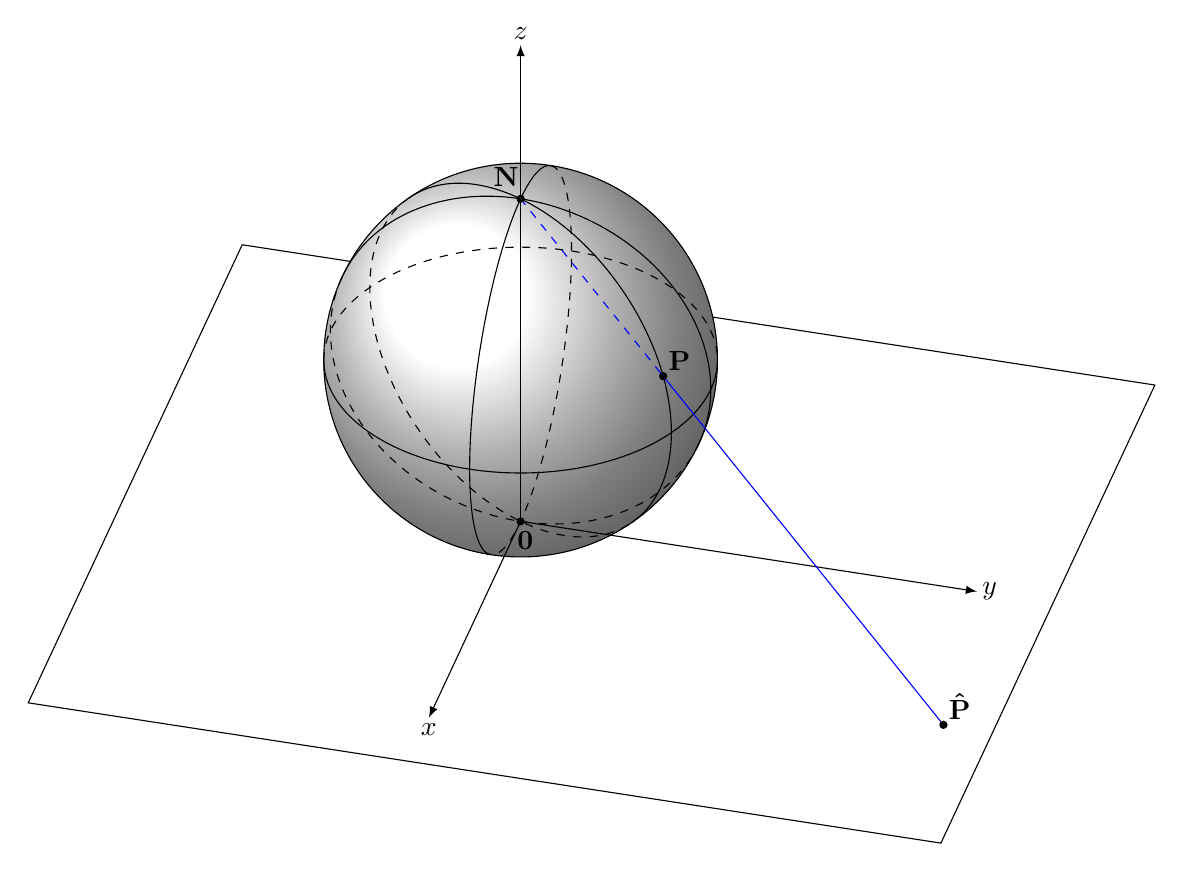
\begin{tikzpicture} % CENT
\newcommand\pgfmathsinandcos[3]{%
  \pgfmathsetmacro#1{sin(#3)}%
  \pgfmathsetmacro#2{cos(#3)}%
}
\newcommand\LongitudePlane[3][current plane]{%
  \pgfmathsinandcos\sinEl\cosEl{#2} % elevation
  \pgfmathsinandcos\sint\cost{#3} % azimuth
  \tikzset{#1/.estyle={cm={\cost,\sint*\sinEl,0,\cosEl,(0,0)}}}
}
\newcommand\LatitudePlane[3][current plane]{%
  \pgfmathsinandcos\sinEl\cosEl{#2} % elevation
  \pgfmathsinandcos\sint\cost{#3} % latitude
  \pgfmathsetmacro\yshift{\cosEl*\sint}
  \tikzset{#1/.estyle={cm={\cost,0,0,\cost*\sinEl,(0,\yshift)}}} %
}
\newcommand\DrawLongitudeCircle[2][1]{
  \LongitudePlane{\angEl}{#2}
  \tikzset{current plane/.prefix style={scale=#1}}
   % angle of "visibility"
  \pgfmathsetmacro\angVis{atan(sin(#2)*cos(\angEl)/sin(\angEl))} %
  \draw[current plane] (\angVis:1) arc (\angVis:\angVis+180:1);
  \draw[current plane,dashed] (\angVis-180:1) arc (\angVis-180:\angVis:1);
}
\newcommand\DrawLatitudeCircle[2][1]{
  \LatitudePlane{\angEl}{#2}
  \tikzset{current plane/.prefix style={scale=#1}}
  \pgfmathsetmacro\sinVis{sin(#2)/cos(#2)*sin(\angEl)/cos(\angEl)}
  % angle of "visibility"
  \pgfmathsetmacro\angVis{asin(min(1,max(\sinVis,-1)))}
  \draw[current plane] (\angVis:1) arc (\angVis:-\angVis-180:1);
  \draw[current plane,dashed] (180-\angVis:1) arc (180-\angVis:\angVis:1);
}

\tikzset{%
  >=latex, % option for nice arrows
  inner sep=0pt,%
  outer sep=2pt,%
  mark coordinate/.style={inner sep=0pt,outer sep=0pt,minimum size=3pt,
    fill=black,circle}%
}
%% some definitions

\def\R{2.5} % sphere radius
\def\angEl{35} % elevation angle
\def\angAz{-105} % azimuth angle
\def\angPhi{-40} % longitude of point P
\def\angBeta{19} % latitude of point P

%% working planes

\pgfmathsetmacro\H{\R*cos(\angEl)} % distance to north pole
\tikzset{xyplane/.estyle={cm={cos(\angAz),sin(\angAz)*sin(\angEl),-sin(\angAz),
                              cos(\angAz)*sin(\angEl),(0,-\H)}}}
\LongitudePlane[xzplane]{\angEl}{\angAz}
\LongitudePlane[pzplane]{\angEl}{\angPhi}
\LatitudePlane[equator]{\angEl}{0}

%% draw xyplane and sphere

\draw[xyplane] (-2*\R,-2*\R) rectangle (2.2*\R,2.8*\R);
\fill[ball color=white] (0,0) circle (\R); % 3D lighting effect
\draw (0,0) circle (\R);

%% characteristic points

\coordinate (O) at (0,0);
\coordinate[mark coordinate] (N) at (0,\H);
\coordinate[mark coordinate] (S) at (0,-\H);
\path[pzplane] (\angBeta:\R) coordinate[mark coordinate] (P);
\path[pzplane] (\R,0) coordinate (PE);
\path[xzplane] (\R,0) coordinate (XE);
\path (PE) ++(0,-\H) coordinate (Paux); % to aid Phat calculation
\coordinate[mark coordinate] (Phat) at (intersection cs: first line={(N)--(P)},
                                        second line={(S)--(Paux)});

%% draw meridians and latitude circles

\DrawLatitudeCircle[\R]{0} % equator
\DrawLongitudeCircle[\R]{\angAz} % xzplane
\DrawLongitudeCircle[\R]{\angAz+90} % yzplane
\DrawLongitudeCircle[\R]{\angPhi} % pzplane

%% draw xyz coordinate system

\draw[xyplane,<->] (1.8*\R,0) node[below] {$x$} -- (0,0) -- (0,2.4*\R)
    node[right] {$y$};
\draw[->] (0,-\H) -- (0,1.6*\R) node[above] {$z$};

%% draw lines and put labels

\draw[blue,dashed] (P) -- (N) +(0.3ex,0.6ex) node[above left,black] {$\mathbf{N}$};
\draw[blue] (P) -- (Phat) node[above right,black] {$\mathbf{\hat{P}}$};
\path (S) +(0.4ex,-0.4ex) node[below] {$\mathbf{0}$};
\draw (P) node[above right] {$\mathbf{P}$};
\end{tikzpicture}
\begin{remarks}
To investigate the properties of $\infty$, use the substitution $\xi=\frac{1}{z}$. A function $f(z)$ has a particular property at $z=\infty$ if $f(1/\xi)$ has that property at $\xi=0$.
\end{remarks}
\subsubsection{Complex differentiation}
\begin{defi}[Complex differentiability]
A complex function $f(z)$ is complex differentiable if the limit
\begin{equation}
f'(z)=\lim_{\delta z\rightarrow 0}\frac{f(z+\delta z)-f(z)}{\delta z}\tag{6.4}
\end{equation}
exists and is independent of the direction of approach. $f'(z)$ is its complex derivative.
\end{defi}
\begin{defi}[Analytic]
We say $f$ is analytic at $z$ if $\exists$ a neighbourhood of $z$ throughout which $f'$ exists.
\end{defi}
\begin{defi}[Entire]
A function is entire if it is analytic throughout $\mathbb{C}$.
\end{defi}
\begin{defi}[Singularity]
A singularity of $f$ is a point at which it is not analytic, or not even defined.
\end{defi}
\begin{remarks}
Analyticity is a strong property with two consequences:
\begin{enumerate}
    \item If a function is analytic, then it is differentiable infinitely many number of times (not true for real functions).
    \item A bounded entire function is constant.
\end{enumerate}
\end{remarks}
\begin{prop}
Suppose $f(z)=u(x,y)+iv(x,y)$ is differentiable at $z=x+iy$, where $x,y\in\mathbb{R}$ and $u(x,y),v(x,y)$ are real-valued functions, then $f$ must satisfy the Cauchy-Riemann equations.
\begin{equation}
\frac{\partial u}{\partial x}=\frac{\partial v}{\partial y},\quad\frac{\partial u}{\partial y}=-\frac{\partial v}{\partial x}\tag{6.5}
\end{equation}
\end{prop}
\begin{proof}
Take $\delta z$ to be $\delta x$ and $i\delta y$ separately, and show $f'(z)$ has the same value regardless of approach.
$$\lim_{\delta x\rightarrow0}\frac{f(z+\delta x)-f(z)}{\delta x}=\lim_{\delta x\rightarrow 0}\frac{u(x+\delta x,y)+iv(x+\delta x,y)-((u(x,y)+iv(x,y))}{\delta x}=\frac{\partial u}{\partial x}+i\frac{\partial v}{\partial x}$$
$$\lim_{\delta y\rightarrow0}\frac{f(z+i\delta y)-f(z)}{i\delta y}=\lim_{\delta y\rightarrow 0}\frac{u(x,y+i\delta y)+iv(x,y+i\delta y)-((u(x,y)+iv(x,y))}{i\delta y}=-i\frac{\partial u}{\partial y}+\frac{\partial v}{\partial y}$$
Comparing them gives the Cauchy-Riemann equations. Denote it as CRE.
\end{proof}
\begin{remarks}
For the converse to be true, i.e. function satisfying CRE must be differentiable, we require the partial derivatives $u_x,u_y,v_x,v_y$ to be differentiable in both $x$ and $y$ together.
\end{remarks}
\begin{eg}\leavevmode
\begin{enumerate}
    \item $f(z)=e^z=e^x(\cos y+i\sin y)$ is entire. $\frac{\partial u}{\partial x}=e^x\cos y=\frac{\partial v}{\partial y}$, $\frac{\partial u}{\partial y}=-e^x\sin y=-\frac{\partial v}{\partial x}$ and hence $f'(z)=\frac{\partial u}{\partial x}+i\frac{\partial v}{\partial x}=e^x\cos y+ie^x\sin y=e^z$ as expected.
    \item If $f(z)$ is analytic and $f(z_0)\neq 0$, then $\frac{1}{f(z)}$ is analytic at $z_0$, so $\frac{1}{z}$ is analytic except at $z=0$.
    \item Any rational function $f(z)=\frac{P(z)}{Q(z)}$, where $P(z)$ and $Q(z)$ are polynomials, is analytic except at points where $Q(z)=0$. For instance, $\frac{z}{z^2+1}$ is analytic except at $z=\pm i$.
    \item Many standard real functions can be extended naturally to complex functions and obey the usual rules for their derivatives. They include polynomials, trigonometric functions, logarithmic functions and hyperbolic functions.
    \item Product/composition of two analytic functions is also analytic. May use product/quotient/chain rules.
\end{enumerate}
\end{eg}
\begin{remarks}
It is sometimes useful to write the complex trigonometric functions as
$$\sin z=\sin(x+iy)=\sin x\cos(iy)+\cos x\sin(iy)=\sin x\cosh y+i\cos x\sinh y$$
\end{remarks}
\begin{eg}
Examples of non-analytic functions are
\begin{enumerate}
    \item $f(z)=|z|$ has $u=\sqrt{x^2+y^2}$, $v=0$ and do not satisfy CRE, so $|z|$ is nowhere analytic. But, let $f(z)=|z|^2=x^2+y^2$, then the CRE is satisfied only at the origin ($2x=0$, $2y=0$), so the function is only differentiable at 0. $|z|^2$ is still nowhere analytic since no neighbourhood of 0 throughout which $f$ is differentiable.
    \item $f(z)=\overline{z}=x-iy$ has $u=x$, $v=-y$ and again do not satisfy CRE. So $\overline{z}$ is nowhere analytic even if $z$ is analytic.
\end{enumerate}
\end{eg}
\subsubsection{Harmonic functions}
\begin{defi}[Harmonic function]
A function satisfying Laplace's equation in some two-dimensional domain is said to be harmonic there.
\end{defi}
\begin{prop}
If $f(z)=u+iv$ is analytic, then it is harmonic.
\end{prop}
\begin{proof} Since $f$ is analytic, it satisfies CRE.
$$\frac{\partial^2u}{\partial x^2}=\frac{\partial }{\partial x}\frac{\partial v}{\partial y}=\frac{\partial}{\partial y}\frac{\partial v}{\partial x}=\frac{\partial}{\partial y}\bigg(-\frac{\partial u}{\partial y}\bigg)=-\frac{\partial^2u}{\partial y^2}$$
And thus $u$ is a solution to Laplace's equation and by definition, it is harmonic. Similar for $v$.
\end{proof}
\begin{defi}[Harmonic conjugate]
$u$, $v$ are said to be harmonic conjugates if they satisfy CRE, i.e. if we know one function then we know the other, up to a constant.
\end{defi}
\begin{eg}
Consider $u(x,y)=x^2-y^2$ (harmonic), $v$ satisfies $\frac{\partial v}{\partial y}=\frac{\partial u}{\partial x}=2x\implies v=2xy+g(x)$, so $-2y=\frac{\partial u}{\partial y}=-\frac{\partial v}{\partial x}=-2y-g'(x)$. So $g(x)$ is a constant, say $\alpha$. Then the corresponding analytic function whose real part is $u$, is thus
$$f(z)=x^2-y^2+2ixy+i\alpha=(x+iy)^2+i\alpha=z^2+i\alpha$$
\end{eg}
\begin{remarks}
If the domain in which the functions are harmonic is not simply connected, then this method might give a solution that is multi-valued. For instances, if $u=\frac{1}{2}\ln|x^2+y^2|$, which is harmonic on $|z|\neq 0$, the corresponding $f(z)=\ln z$, which is multi-valued. See Section 1.4.
\end{remarks}
\begin{prop}
Contours of harmonic conjugate functions are perpendicular to each other.
\end{prop}
\begin{proof}
The gradient $\boldsymbol{\nabla}u=(\frac{\partial u}{\partial x},\frac{\partial u}{\partial y})^T$ is perpendicular to contours of $u$ (curves of constant $u$). Similar for $v$, then
$$\boldsymbol{\nabla}u\cdot\boldsymbol{\nabla}v=\frac{\partial u}{\partial x}\frac{\partial v}{\partial x}+\frac{\partial u}{\partial y}\frac{\partial v}{\partial y}=\frac{\partial u}{\partial x}\bigg(-\frac{\partial u}{\partial y}\bigg)+\frac{\partial u}{\partial y}\frac{\partial u}{\partial x}=0$$
where we used the CRE, and so the result follows.
\end{proof}
\begin{prop}\leavevmode
\begin{enumerate}
    \item Every stationary point of $u$ is a stationary point of $v$ and vice-versa.
    \item Stationary points for which
        $\begin{vmatrix}\partial_{xx}u&\partial_{xy}u\\\partial_{yx}u&\partial_{yy}u\\\end{vmatrix}\neq0$ must be saddle points.
\end{enumerate}
\end{prop}
\begin{proof}\leavevmode
\begin{enumerate}
    \item If we have a stationary point of $u$, then $\frac{\partial u}{\partial x}=\frac{\partial u}{\partial y}=0$. By CRE, then $\frac{\partial v}{\partial x}=\frac{\partial v}{\partial y}=0$, and hence a stationary point of $v$.
    \item Evaluating the Hessian, we have
$$\frac{\partial}{\partial x}\frac{\partial u}{\partial x}\times\frac{\partial}{\partial y}\frac{\partial u}{\partial y}-\bigg(\frac{\partial^2u}{\partial x\partial y}\bigg)^2=-\bigg(\frac{\partial^2v}{\partial x\partial y}\bigg)^2-\bigg(\frac{\partial^2u}{\partial x\partial y}\bigg)^2<0$$
For a function of 2 variables $u(x,y)$, if the determinant of the Hessian is negative at this point, this point is a saddle point.
\end{enumerate}
\end{proof}
\begin{cor}
If $f(z)=u(x,y)+iv(x,y)$ and $g(z)=s(x,y)+it(x,y)$ are analytic functions, then so is $g(f(z))$, and hence deduce that $s(u(x,y),v(x,y))$ satisfies Laplace's equation.
\end{cor}
\begin{proof}
We have $f(x+iy)=u(x,y)+iv(x,y)$ to be analytic, then $f$ satisfies the CRE, i.e. $(\frac{\partial u}{\partial x})_y=(\frac{\partial v}{\partial y})_x$ and $(\frac{\partial u}{\partial y})_x=-(\frac{\partial v}{\partial x})_y$. Similarly, $g(u+iv)=s(u,v)+it(u,v)$ is analytic, this gives $(\frac{\partial s}{\partial v})_u=(\frac{\partial t}{\partial v})_u$ and $(\frac{\partial s}{\partial v})_u=-(\frac{\partial t}{\partial u})_v$. Consider the composite function
$$g(f(z))=s(u(x,y),v(x,y))+it(u(x,y),v(x,y))$$
then we have by chain rule,
$$\bigg(\frac{\partial s}{\partial x}\bigg)_y=\bigg(\frac{\partial u}{\partial x}\bigg)_y\bigg(\frac{\partial s}{\partial u}\bigg)_v+\bigg(\frac{\partial v}{\partial x}\bigg)_y\bigg(\frac{\partial s}{\partial v}\bigg)_u=\bigg(\frac{\partial v}{\partial y}\bigg)_x\bigg(\frac{\partial t}{\partial v}\bigg)_u+\bigg(\frac{\partial t}{\partial u}\bigg)_v\bigg(\frac{\partial u}{\partial y}\bigg)_x=\bigg(\frac{\partial t}{\partial y}\bigg)_x$$
$$\bigg(\frac{\partial s}{\partial y}\bigg)_x=\bigg(\frac{\partial u}{\partial y}\bigg)_x\bigg(\frac{\partial s}{\partial u}\bigg)_v+\bigg(\frac{\partial v}{\partial y}\bigg)_x\bigg(\frac{\partial s}{\partial v}\bigg)_u=-\bigg(\frac{\partial v}{\partial x}\bigg)_y\bigg(\frac{\partial t}{\partial v}\bigg)_u-\bigg(\frac{\partial t}{\partial u}\bigg)_v\bigg(\frac{\partial u}{\partial x}\bigg)_y=\bigg(\frac{\partial t}{\partial x}\bigg)_y$$
Hence composite functions obey the CRE and $s(u,v)$ is thus harmonic and also satisfy the Laplace's equation.
\end{proof}
\subsubsection{Zeros}
\begin{defi}[Zero]
The zeros of an analytic function $f$ are the points $z_0$ where $f(z_0)=0$. A zero is of order $N$ if, in its Taylor series $\sum_na_n(z-z_0)^n$, the first non-zero coefficient is $a_N$. Alternatively, it is of order $N$ if $0=f(z_0)=f'(z_0)=\dots f^{(N-1)}(z_0)$ but $f^{(N)}(z_0)\neq 0$. In particular, a zero of order 1 is called a simple zero.
\end{defi}
\begin{eg}\leavevmode
\begin{enumerate}
    \item $z^3+iz^2+z+i=(z-i)(z+i)^2$ has a simple zero at $z=i$ and a zero of order 2 at $z=-i$.
    \item $\sinh z$ has zeroes where $\frac{e^z-e^{-z}}{2}=0\iff e^{2z}=1\iff z=n\pi i,n\in\mathbb{Z}$. The zeros are all simple since its derivative $\cosh(n\pi i)=\cos(n\pi)\neq 0$.
    \item Since $\sinh z$ has a simple zero at $z=\pi i$, $\sinh^3z$ has a zero of order 3 there. If needed, we can find its Taylor series about $\pi i$ by visiting $\xi=z-\pi i$:
    $$\sinh^3z=\sinh^3(\xi+\pi i)=(-\sinh\xi)^3=-(\xi+\frac{1}{3!}\xi^3+\dots)^3=-(z-\pi i)^3-\frac{1}{2}(z-\pi i)^5-\dots$$
    where we used the standard Taylor series for $\sinh z$.
\end{enumerate}
\end{eg}
\subsubsection{Laurent series}
If $f$ might have a singularity at $z_0$, then we cannot necessarily expect it to have a Taylor series there.
\begin{defi}[Laurent series]
If $f$ is analytic in an annulus $R_1<|z-z_0|<R_2$, then it has a Laurent series about $z_0$, of the form
\begin{equation}
f(z)=\sum_{n=-\infty}^\infty a_n(z-z_0)^n\tag{6.6}
\end{equation}
which is convergent within the annulus.
\end{defi}
\begin{remarks}\leavevmode
\begin{enumerate}
    \item We can show that Laurent series for $f$ about a particular $z_0$ is unique with any given annulus
    \item Taylor series is just a special case of Laurent series, with $a_n=0$ $\forall n<0$ and $R_1=0$. The radius of convergence of a Taylor series is always the distance to the nearest singularity.
\end{enumerate}
\end{remarks}
\begin{eg}\leavevmode
\begin{enumerate}
    \item $\frac{e^z}{z^3}$ has a Laurent series about $z_0=0$ given by
    $$\frac{e^z}{z^3}=\sum_{m=0}^\infty\frac{z^{m-3}}{m!}=\sum_{n=3}^\infty\frac{z^n}{(n+3)!}$$
    so $a_n=\frac{1}{(n+3)!}$ for $n\geq-3$.
    \item $e^{1/z}$ has a Laurent series about $z_0=0$ given by
    $$e^{1/z}=1+\frac{1}{z}+\frac{1}{2!z^2}+\frac{1}{3!z^3}$$
    so $a_n=\frac{1}{(-n)!}$ for $n\leq 0$.
    \item $f(z)=\frac{e^z}{z^2-1}$ has a singularity at $z_0=1$ but is analytic in the annulus $0<|z-z_0|<2$ (since the only singularities are at $\pm 1$). Write everything in $\xi=z-z_0$, so $f(z)$ is
    $$\frac{e^\xi e^{z_0}}{\xi(\xi+2)}=\frac{e^{z_0}}{2\xi}e^\xi(1+0.5\xi)^{-1}=\frac{e^{z_0}}{2\xi}(1+\xi+\frac{1}{2!}\xi^2+\dots)(1-0.5\xi+0.25\xi^2+\dots)=\frac{e^{z_0}}{2\xi}(1+0.5\xi+0.25\xi^2+\dots)$$
    which gives $\frac{1}{2}e^{z_0}(\frac{1}{z-z_0}+\frac{1}{2}+\frac{z-z_0}{4}+\dots)$. Hence $a_{-1}=\frac{1}{2}e$, $a_0=\frac{1}{4}e$, etc. This series is valid in the whole annulus (our expansion of $(1+0.5\xi)^{-1}$ was valid for $|0.5\xi|<1$, i.e. $|z-z_0|<2$).
    \item If $f(z)=\frac{1}{z-a}$ for $a\in\mathbb{C}$, then it is analytic in $|z|<|a|$, so it has a Taylor series about $z_0=0$ given by
    $$\frac{1}{z-a}=-\frac{1}{a}\bigg(1-\frac{z}{a}\bigg)^{-1}=-\sum_{n=0}^\infty a^{-n-1}z^n$$
    where the binomial expansion is valid since $|\frac{z}{a}|<1$. In $|z|>|a|$, it has a Laurent series in the annulus $|a|<|z|<\infty$, given by
    $$\frac{1}{z-a}=\frac{1}{z}\bigg(1-\frac{a}{z}\bigg)^{-1}=\sum_{m=0}^\infty\frac{a^m}{z^{m+1}}=\sum_{n=-\infty}^{-1}a^{-n-1}z^n$$
    where the binomial expansion is valid since $|\frac{a}{z}|<1$.
    \item This doesn't seem to work for $f(z)=z^{-1/2}$. We cannot find a Laurent series about $z_0=0$. The reason is the required branch cut would pass through any annulus about 0, so cannot find such an annulus in which $f$ is analytic. (Of course, $z^{-1/2}$ has a Taylor series about other points $z_0\neq 0$, except those on the branch cut).
\end{enumerate}
\end{eg}
\begin{remarks}[Radius of convergence]
Suppose we have a Laurent series that we know to be valid in annulus $R_1<|z-z_0|<R_2$, but there are no singularities on $|z-z_0|=R_2$. Then the outer radius of convergence can actually be pushed outwards until the circle touches a singularity, say $z_2$.\\[5pt]
Similarly, if no singularity in $|z-z_0|=R_1$, the inner radius can be pulled in until we encounter a singularity, say $z_1$. Then our Laurent series in fact converges in the enlarged annulus
$$\{z:~|z_1|=R_1'<|z-z_0|<R_2'=|z_2|\}$$
In other words, the annulus of convergence of a Laurent series is always maximally large, with a singularity on each of the bounding circles, even if we originally derived it in a smaller region. By Remarks 3.1.1, the new Laurent series must be the same as the old one, noting that they have an overlap region where they are both valid.
\end{remarks}
\begin{eg}
$\cosec z$ has a Laurent series
$$\bigg(z-\frac{z^3}{3!}+\dots\bigg)^{-1}=z^{-1}\bigg(1-\frac{z^2}{6}+\dots\bigg)^{-1}=z^{-1}+\frac{z}{6}+\dots$$
for sufficiently small $z\neq 0$, but it is not immediately obvious when the binomial expansion will be valid. The singularities of $\cosec z$ closest to 0 are at $z=\pm\pi$, so the radius of convergence is in fact $0<|z|<\pi$.
\end{eg}
\newpage
\subsubsection{Classification of singularities}
\begin{defi}[Isolated singularity]
Suppose $f$ has a singularity at $z=z_0$. If there is a neighbourhood of $z_0$ in which $f$ is analytic (except at $z_0$) then $f$ has an isolated singularity at $z_0$. Otherwise, we call it a non-isolated singularity.
\end{defi}
\begin{eg}\leavevmode
\begin{enumerate}
    \item $\cosech z$ has an isolated singularity at $z=n\pi i$, $n\in\mathbb{Z}$.
    \item $\cosech\frac{1}{z}$ has an isolated singularity at $z=\frac{1}{n\pi i}$, $n\neq 0$ and a non-isolated singularity at $z=0$ (since there are other arbitrarily close singularities, i.e. $n$ large).
    \item $\cosech z$ has a non-isolated singularity at $\infty$.
    \item $z^{-1/2}$ has a branch point singularity at $z=0$. This is a type of non-isolated singularity since $z^{-1/2}$ is not analytic at any point on the branch cut. We usually treat this as a separate case.
\end{enumerate}
\end{eg}
\begin{defi}[Removable singularity]
If $f$ has a removable singularity at $z_0$, then $\lim_{z\rightarrow z_0}f(z)$ is finite, i.e. $f(z)=a_0+a_1(z-z_0)+\dots$ for $0<|z-z_0|<r_0$ s.t. $\lim_{z\rightarrow z_0}f(z)=a_0$. Then, we can `remove the singularity' by redefining $f(z_0)$ as $a_0$. Then $f$ will become analytic at $z_0$.
\end{defi}
\begin{defi}[Pole]
If $f$ has a pole at $z_0$, then $\lim_{z\rightarrow z_0}|f(z)|=\infty$.
\end{defi}
\begin{defi}[Essential isolated singularity]
If $f$ has an essential isolated singularity, $f$ does not tend to any finite or infinite limit at this point.
\end{defi}
\begin{remarks}
If $f$ has an isolated singularity at $z_0$, we can find an annulus $0<|z-z_0|<r_0$ say within which $f$ is analytic and therefore has a Laurent series. This gives a way to classify singularities.
\begin{enumerate}
    \item Check for a branch point singularity.
    \item Check for a non-isolated singularity.
    \item Otherwise, consider the coefficients of Laurent series $\sum_{n=-\infty}^\infty a_n(z-z_0)^n$:
    \begin{itemize}
        \item If $a_n=0$ $\forall n<0$, then $f$ has a removable singularity at $z_0$.
        \item If $\exists N>0$ s.t. $a_n=0$ $\forall n<-N$, but $a_{-N}\neq 0$, then $f$ has a pole of order $N$ at $z_0$ (simple pole at $N=1$, double pole at $N=2$, etc).
        \item If there is no such $N$, then $f$ has an essential isolated singularity,
    \end{itemize}
\end{enumerate}
In fact, we can show that $f$ takes all possible complex values (except at most one) in any neighbourhood of $z_0$, however small. For instance, $e^{1/z}$ takes all values except 0.
\end{remarks}
\begin{prop}\leavevmode
\begin{enumerate}
    \item If $g(z)$ has a zero of order $N$ at $z_0$, then $\frac{1}{g(z)}$ has a pole of order $N$ there.
    \item A rational function $f(z)=\frac{P(z)}{Q(z)}$ where $P$ and $Q$ are polynomials in $z$, has a singularity at any $z_0$, where $Q$ has a zero. But if $P(z_0)=0$ as well and assuming $Q$ has a simple zero, then the singularity is removable by redefining $f(z_0)=\frac{P'(z_0)}{Q'(z_0)}$.
\end{enumerate}
\end{prop}
\newpage
\begin{eg}\leavevmode
\begin{enumerate}
    \item $\frac{\cos z}{z}$ has Laurent series $z^{-1}-\frac{1}{2}z+\frac{1}{24}z^3+\dots$ about $z=0$ so has a simple pole at 0.
    \item $\frac{1}{z-i}$ has a simple pole at $z=i$, since it is its own Laurent series.
    \item $\frac{z^2}{(z-1)^2(z-i)^3}$ has a double pole at $z=1$ and triple pole at $z=i$. To show formally that, for instance, there is a double pole at $z=1$, note $\frac{z^2}{(z-i)^3}$ is analytic there, so has a Taylor series $b_0+b_1(z-1)+b_2(z-1)^2+\dots$ for some $b_n$. Hence,
    $$\frac{z^2}{(z-1)^2(z-i)^3}=\frac{b_0}{(z-1)^2}+\frac{b_1}{z-1}+b_2+\dots$$
    \item $\cot z$ has a simple pole at 0, since $\tan z$ has a simple zero there.
    \item $z^2$ has a double pole at $\infty$.
    \item $e^{1/z}$ has an essential isolated singularity at 0 because $a_n\neq 0$ for $n\leq 0$.
    \item $\sin\frac{1}{z}$ also has an essential isolated singularity at $z=0$ because using the standard Taylor series for $\sin$, there are non-zero $a_n$ for infinitely many negative $n$.
    \item $f(z)=\frac{e^z-1}{z}$ has a removable singularity at 0 since $f(z)=1+\frac{1}{2!}z+\frac{1}{3!}z^2+\dots$. By defining $f(0)=1$, we would remove the singularity and obtain an entire function.
    \item $f(z)=\frac{\sin z}{z}$ is not defined at 0, but has a removable singularity there. Remove it by defining $f(0)=1$.
\end{enumerate}
\end{eg}
\newpage
\section{Series solutions to ODEs}
{\small\textcolor{darkblue}{Homogeneous equations; solution by series (without full discussion of logarithmic singularities), exemplified by Legendre's equation. Classification of singular points. Indicial equation and local behaviour of solutions near singular points.}\hfill\textbf{[3]}}\\[5pt]
We will consider series solutions to the equations of the form
\begin{equation}
  p(x) y'' + q(x) y' + r(x) y = 0\tag{7.1}
\end{equation}
\begin{defi}[Ordinary and singular points]
  The point $x = x_0$ is an ordinary point of the differential equation if $\frac{q}{p}$ and $\frac{r}{p}$ have Taylor series about $x_0$. Otherwise, $x_0$ is a singular point.\\[5pt]
  If $x_0$ is a singular point but the equation can be written as
\begin{equation}  
P(x)(x - x_0)^2y'' + Q(x)(x - x_0)y' + R(x)y = 0\tag{7.2}
\end{equation}
  where $\frac{Q}{P}$ and $\frac{R}{P}$ have Taylor series about $x_0$, then $x_0$ is a regular singular point.
\end{defi}

\begin{eg}\leavevmode
  \begin{enumerate}
    \item $(1 - x^2)y'' - 2cy' + 2y = 0$. $x = 0$ is an ordinary point. However, $x = \pm 1$ are (regular) singular points since $p(\pm 1) = 0$.
    \item $\sin x y'' + \cos x y' + 2y = 0$. $x = n\pi$ are regular singular points while all others are ordinary.
    \item $(1 + \sqrt{x}) y'' - 2xy' + 2y = 0$. $x = 0$ is an irregular singular point because $\sqrt{x}$ is not differentiable at $x = 0$.
  \end{enumerate}
\end{eg}
\begin{prop}
If $x_0$ is
\begin{itemize}
    \item an ordinary point, then the equation is guaranteed to have two linearly independent solutions of the form $y=\sum_{n=0}^\infty a_n(x-x_0)^n$, i.e. Taylor series about $x_0$. The solution must be convergent in some neighbourhood of $x_0$;
    \item a regular singular point, then there is at least one solution of the form $y=\sum_{n=0}^\infty a_n(x-x_0)^{n+\sigma}$, i.e. Frobenius series about $x_0$ where $a_0\neq 0$ to ensure the index $\sigma\in\mathbb{C}$ is unique.
\end{itemize}
\end{prop}
\subsection{Ordinary points}
\begin{eg}[Ordinary point]
  Consider $(1 - x^2)y'' - 2xy' + 2y = 0$. Find a series solution about $x = 0$ (which is an ordinary point).

  We try $y = \sum_{n = 0}^\infty a_nx^n$ and compare the coefficient of $x^n$ and obtain the following general recurrence relation:
  $$0=n(n - 1) a_n + [-(n - 2)^2 - (n - 2) + 2]a_{n - 2}=n(n - 1)a_n- (n^2 - 3n)a_{n - 2}$$
  Here we do not divide by anything since they might be zero.\\[5pt]
  First consider the case $n = 0$. The left hand side gives $0\cdot a_0 = 0$ (the right hand side is $0$ since $a_{n - 2} = 0$). So any value of $a_0$ satisfies the recurrence relationship, and it can take any arbitrary value. This corresponds to a constant of integration. Similarly, by considering $n = 1$, $a_1$ is arbitrary. For $n > 1$, $n$ and $n - 1$ are non-zero. So we have
  \begin{align*}
    a_n &= \frac{n - 3}{n - 1} a_{n - 2}\\
    \intertext{In this case (but generally not), we can further simplify it to obtain:}
    a_{2k} &= \frac{-1}{2k - 1}a_0,\\
    a_{2k + 1} &= 0.
  \end{align*}
  So we obtain
  \begin{align*}
    y &= a_0[1 - \frac{x^2}{1} - \frac{x^4}{3} - \frac{x^6}{5} - \cdots] + a_1 x\\
    &= a_0\left[1 - \frac{x}{2}\ln\left(\frac{1 + x}{1 - x}\right)\right] + a_1x
  \end{align*}
  Notice the logarithmic behaviour near $x = \pm 1$ which are regular singular points.
\end{eg}

\subsection{Regular singular points}
\begin{eg}[Regular singular point]
  Consider $4xy'' + 2(1 - x^2)y' - xy = 0$. Note that $x = 0$ is a singular point. But since $\frac{Q}{P} = \frac{1 - x^2}{2}$ and $\frac{R}{P} = -\frac{x^2}{4}$ both have Taylor series, $x = 0$ is a regular singular point. Try $y=\sum_{n=0}^\infty a_nx^{n+\sigma}$ with $a_0\neq 0$ and comparing the coefficient of $x^{n + \sigma}$, we obtain the general recurrence relation
  \[
    [4(n + \sigma)(n + \sigma - 1) + 2(n + \sigma)]a_n -[2(n - 2 + \sigma) + 1]a_{n - 2} = 0\implies 
    2(n + \sigma)(2n + 2\sigma - 1)a_n = (2n + 2\sigma-3)a_{n - 2}.
  \]
  The $n = 0$ case gives the indicial equation for the index $\sigma$:
  \[
    2\sigma(2\sigma - 1)a_0 = 0.
  \]
  Since $a_0 \not= 0$, we must have $\sigma = 0$ or $\frac{1}{2}$. The $\sigma = 0$ solution corresponds to an analytic (``Taylor series'') solution, while $\sigma = \frac{1}{2}$ corresponds to a non-analytic one.\\[5pt]
  When $\sigma = 0$, the recurrence relation becomes
  \[
    2n(2n - 1)a_n = (2n - 3)a_{n - 2}.
  \]
  When $n = 0$, this gives $0\cdot a_0 = 0$. So $a_0$ is arbitrary. For $n >0$, we can divide and obtain
  \[
    a_n = \frac{2n - 3}{2n(2n - 1)}a_{n - 2}.
  \]
  We can see that $a_1 = 0$ and so are subsequent odd terms.   If $n = 2k$, i.e.\ $n$ is even, then
  \begin{align*}
    a_{2k} &= \frac{4k - 3}{4k(4k - 1)}a_{2k - 2}\\
    y &= a_0\left[1 + \frac{1}{4\cdot 3}x^2 + \frac{5}{8\cdot 7\cdot 4\cdot 3}x^4 + \cdots\right]
  \end{align*}
  Note that we have only found one solution in this case. 
  Now when $\sigma = \frac{1}{2}$, we obtain
  \[
    (2n + 1)(2n)a_n = (2n - 2)a_{n - 2}
  \]
  When $n = 0$, we obtain $0\cdot a_0 = 0$, so $a_0$ is arbitrary. To avoid confusion with the $a_0$ above, call it $b_0$ instead.  When $n = 1$, we obtain $6a_1 = 0$ and $a_1 = 0$ and so are subsequent odd terms.  For even $n$,
  \[
    a_n = \frac{n - 1}{n(2n + 1)}a_{n - 2}
  \]
  So
  \[
    y = b_0 x^{1/2}\left[1 + \frac{1}{2\cdot 5}x^2 + \frac{3}{2\cdot 5\cdot 4\cdot 9}x^4 + \cdots\right]
  \]
\end{eg}

\subsection{Resonance of solutions}
Note that the indicial equation has two roots $\sigma_1, \sigma_2$. Consider the two different cases:
\begin{enumerate}
  \item If $\sigma_2 - \sigma_1\notin\mathbb{Z}$, then there are two linearly independent Frobenius solutions
    \[
      y = \left[(x - x_0)^{\sigma_1}\sum_{n = 0}^{\infty} a_n(x - x_0)^n\right] + \left[(x - x_0)^{\sigma_2}\sum_{n = 0}^{\infty} b_n(x - x_0)^n\right].
    \]
    As $x\to x_0$, $y \sim (x - x_0)^{\sigma_1}$, where $\Re(\sigma_1) \leq \Re(\sigma_2)$

  \item If $\sigma_2 - \sigma_1\in\mathbb{Z}$ (including when they are equal), there is one solution of the form
    \[
      y_1 = (x - x_0)^{\sigma_2}\sum_{n = 0}^{\infty} a_n(x - x_0)^n
    \]
    with $\sigma_2 \geq \sigma_1$. In this case, $\sigma = \sigma_1$ will not give a valid solution, as we will later see. Instead, the other solution is (usually) in the form
    \[
      y_2 = \ln(x - x_0)y_1 + \sum_{n = 0}^\infty b_n(x - x_0)^{n + \sigma_1}.
    \]
    This form arises from resonance between the two solutions. But if the resonance somehow avoids itself, we can possibly end up with two regular Frobenius series solutions.

    We can substitute this form of solution into the differential equation to determine $b_n$.
\end{enumerate}
\begin{eg}[Regular singular point with logarithmic solution]
  Consider $x^2 y'' - xy = 0$. $x = 0$ is a regular singular point. It is already in equidimensional form $(x^2y'') - x(y) = 0$. Try
  \[
    y = \sum_{n = 0}^\infty a_n x^{n + \sigma}
  \]
  with $a_0 \not= 0$. We obtain
  \[
    \sum a_nx^{n + \sigma}[(n + \sigma)(n + \sigma - 1) - x] = 0.
  \]
  The general recurrence relation is
  \[
    (n + \sigma)(n + \sigma - 1)a_n = a_{n - 1}.
  \]
  $n = 0$ gives the indicial equation
  \[
    \sigma(\sigma - 1) = 0.
  \]
  Then $\sigma = 0, 1$. We are guaranteed to have a solution in the form $\sigma = 1$. When $\sigma = 1$, the recurrence relation becomes
  \[
    (n + 1)n a_n = a_{n - 1}.
  \]
  When $n = 0$, $0\cdot a_0 = 0$ so $a_0$ is arbitrary.
  When $n > 0$, we obtain
  \[
    a_n = \frac{1}{n(n +1)}a_{n - 1} = \frac{1}{(n + 1)(n!)^2}a_0.
  \]
  So
  \[
    y_1 = a_0x\left(1 + \frac{x}{2} + \frac{x^2}{12} + \frac{x^3}{144} + \cdots \right).
  \]
  When $\sigma = 0$, we obtain
  \[
    n(n - 1)a_n = a_{n - 1}.
  \]
  When $n = 0$, $0\cdot a_0 = 0$ and $a_0$ is arbitrary. When $n = 1$, $0\cdot a_1 = a_0$. However, $a_0\not= 0$ by our initial constraint. Contradiction. So there is no solution in this form (If we ignore the constraint that $a_0\not= 0$, we know that $a_0$ is arbitrary. But this gives exactly the same solution we found previously with $\sigma = 1$). The other solution is thus in the form
  \[
    y_2 = y_1\ln x + \sum_{n = 0}^\infty b_nx^n.
  \]
\end{eg}


\newpage
\section{Sturm-Liouville theory}
{\small\textcolor{darkblue}{Self-adjoint operators, eigenfunctions and eigenvalues, reality of eigenvalues and orthogonality of eigenfunctions. Eigenfunction expansions and determinantion of coefficients. Legendre polynomials; orthogonality}

\hfill\textbf{[3]}}
\subsection{Review of 2nd order linear ODEs}
We wish to solve the general inhomogeneous ODE
\begin{equation}
    \mathcal{L}y=\alpha(x)y''+\beta(x)y'+\gamma(x)y=f(x)\tag{8.1}
\end{equation}
The homogeneous equation
\begin{equation}
    \mathcal{L}y=0\tag{8.2}
\end{equation}
has two independent solutions $y_1(x)$, $y_2(x)$ (besides the trivial solution $y=0$), the complementary function $y_c(x)$ is a general solution of (1.28):
\begin{equation}
y_c(x)=Ay_1(x)+By_2(x)\tag{8.3}
\end{equation}
where $A$ and $B$ are arbitrary constants. The inhomogeneous equation
\begin{equation}
    \mathcal{L}y=f(x)\tag{8.4}
\end{equation}
is solved by the particular integral $y_p(x)$. So the general solution of (8.4) is then
\begin{equation}
    y(x)=y_p(x)+Ay_1(x)+By_2(x)\tag{8.5}
\end{equation}
The boundary or initial data are required to determine $A,B$ in (8.5).
\begin{itemize}
    \item b.c.s: solve (8.4) on $a<x<b$ given 
    \begin{itemize}
        \item Dirichlet:
    $y$ at $x=a,b$
    \item Neumann:
    $y'$ at $x=a,b$
    \item Cauchy (mixed):
    $y+ky'=0$
    \end{itemize}
    Homogeneous b.c.s are often assumed, $y(a)=y(b)=0$. This can always be achieved by adding complementary functions (8.3), i.e. $\tilde{y}(x)=y(x)+Ay_1(x)+By_2(x)$, s.t. $\tilde{y}(a)=\tilde{y}(b)=0$.
    \item i.c.s: solve (8.4) for $x\geq a$, given $y,y'$ at $x=a$.
\end{itemize}
To solve (8.1) using eigenfunction expansions, we must first solve the related eigenvalue problem
\begin{equation}
    \alpha(x)y''+\beta y'(x)+\gamma(x)y=-\lambda\rho(x)y\tag{8.6}
\end{equation}
with specified b.c.s. This form occurs after invoking separation of variables in several dimensions.
\subsection{Self-adjoint operators}
\begin{defi}[Weighted inner product]
Define inner product between two continuous complex-valued functions $f,g$ w.r.t the weight function $w(x)$ on $a\leq x\leq b$ to be
\begin{equation}
\langle f,g\rangle_w=\int_a^bw(x)f^*(x)g(x)dx=\langle wf,g\rangle=\langle f,wg\rangle\tag{8.7}
\end{equation}
The weight function $w(x)$ is a real-valued, non-negative function that has at most finitely many zeroes on the domain $[a,b]$.
\end{defi}
\begin{defi}[Norm]
The norm of a complex-valued function w.r.t some weight function $w(x)$ is
$$||f||_w:=\sqrt{\langle f,f\rangle_w}$$
Since $f$ is continuous and $w$ has finitely many zeroes on $[a,b]$, $\langle f,f\rangle_w=0$ iff $f(x)=0$ identically on $[a,b]$.
\end{defi}
\begin{defi}[Self-adjoint]
$\mathcal{L}$ is said to be self-adjoint on $a\leq x\leq b$ $\forall$ functions $y_1,y_2$ satisfying appropriate b.c.s, if
\begin{equation}
    \langle y_1,\mathcal{L}y_2\rangle=\langle\mathcal{L}y_1,y_2\rangle,\text{ i.e.}\quad \int_a^by_1^*(x)\mathcal{L}y_2(x)dx=\int_a^b(\mathcal{L}y_1(x))^*y_2(x)dx\tag{8.8}
\end{equation}
\end{defi}
\begin{defi}[Sturm-Liouville equation]
When $\mathcal{L}$ is self-adjoint, then the eigenvalue problem (8.6) can be expressed in Sturm-Liouville (SL) form
\begin{equation}
    \mathcal{L}y:=-(p y')'+qy=\lambda wy\tag{8.9}
\end{equation}
where the weight function $w(x)\geq 0$ $\forall x$.
\end{defi}
\begin{prop}
The eigenvalue problem (8.6) can be recasted to SL form as long as suitable b.c.s are satisfied.
\end{prop}
\begin{proof}
Multiply (8.6) by an integration factor $\mu(x)$ to find
$$-\lambda\mu\rho y=\mu\alpha y''+\mu\beta y'+\mu\gamma y=(\mu\alpha y')'+y'(-\mu'\alpha-\mu\alpha'+\mu\beta)y'+\mu\gamma y$$
Eliminate the $y'$ term in order to cast it to SL form,
\begin{equation}
\frac{1}{\mu(x)}\frac{d\mu}{dx}=\frac{\beta-\alpha'}{\alpha}\implies\mu(x)=\exp\bigg(\int^x\frac{\beta-\alpha'}{\alpha}dx\bigg)\tag{8.10}
\end{equation}
In that case, $p(x):=\mu(x)\alpha(x)$, $q(x):=-\mu(x)\gamma(x)$, $w(x)=\mu(x)\rho(x)$. Note, $\mu(x)\geq0$. In order to ensure $\mathcal{L}$ is self-adjoint on $a\leq x\leq b$ $\forall$ eigenfunctions $y_1,y_2$, we require it to satisfy (8.8), so
\begin{align}
\langle y_1,\mathcal{L}y_2\rangle-\langle\mathcal{L}y_1,y_2\rangle&=\int_a^b(-y_1(p y_2')'+y_1qy_2+y_2(py_1')'-y_2qy_1)dx\nonumber\\&=\int_a^b(-(p y_1y_2')'+(p y_1'y_2)')dx\nonumber\\&=[-p y_1y_2'+p y_1'y_2]_a^b=0\tag{8.11}
\end{align}
The self-adjoint compatible b.c.s include
\begin{itemize}
    \item homogneneous b.c.s $y(a)=y(b)=0$ or $y'(a)=y'(b)=0$, or mixed $y+ky'=0$, etc;
    \item periodic $y(a)=y(b)$;
    \item singular points of ODE $p(a)=p(b)=0$;
    \item combinations of the above.
\end{itemize}
\end{proof}
\begin{thm}
For self-adjoint operators $\mathcal{L}$,
\begin{enumerate}
    \item the eigenvalues $\lambda_n$ are real,
    \item the eigenfunctions $y_n$ are orthogonal w.r.t the weight function $w(x)$;
    \item  the eigenfunctions $y_n$ form a complete set.
\end{enumerate}
\end{thm}
\begin{proof}
We shall not prove the third part. For the first two, consider two eigenfunctions $y_n,y_m$ with eigenvalues $\lambda_n,\lambda_m$ respectively, i.e.
\begin{equation}
    \mathcal{L} y_{n,m}=\lambda_{n,m}wy_{n,m}\tag{8.12}
\end{equation}
Consider
$$\int_a^b(y_m^*\mathcal{L}y_n-y_n\mathcal{L}y_m)dx=(\lambda_n-\lambda_m^*)\int_a^bwy_ny_mdx$$
LHS is zero by (8.12). When $n=m$, RHS is $(\lambda_n-\lambda_n^*)\int_a^bw|y_n|^2dx$, but $\int w|y_n|^2dx\geq0$ for $y_n\neq 0$, so $\lambda_n=\lambda_n^*\in\mathbb{R}$, i.e. real eigenvalues. In particular, if $\lambda_n$ are non-degenerate, then $y_n^*=y_n$ are real eigenfunctions.\\[5pt]
If $m\neq n$ s.t. the eigenvalues are distinct, i.e. $\lambda_m\neq\lambda_n$, then \begin{equation}
     \int_a^bwy_ny_mdx=0\quad\forall n\neq m\tag{8.13}
\end{equation}
i.e. $y_m$ and $y_n$ are orthogonal w.r.t the weight function $w(x)$ on $a\leq x\leq b$.
\end{proof}
\begin{remarks}\leavevmode
\begin{itemize}
    \item One can show that the regular SL problem (homogeneous b.c.s) has simple eigenvalues $\lambda_n$, i.e. unique eigenfunctions. This is done by considering two eigenfunctions $u,v$ with the same eigenvalue $\lambda$ and use
    $$u\mathcal{L}v-(\mathcal{L}u)v=[-p(uv'-u'v)]'$$
    \item We can eliminate the weight function $w(x)$ by redefining $\tilde{y}=\sqrt{w}y$ and replacing $\mathcal{L}y$ by $\frac{1}{\sqrt{w}}\mathcal{L}\frac{\tilde{y}}{\sqrt{w}}$ but it is generally simpler to keep it.
\end{itemize}
\end{remarks}
\begin{eg}
Consider the Hermite equation for simple harmonic oscillator:
$$y''-2xy'+2ny=0$$
We wish to cast it to SL form (8.9). Compare with (8.6), $\alpha=1$, $\beta=-2x$, $\gamma=0$, $\lambda\rho=2n$. By (8.10), the integration factor is $\exp(\int^x-2xdx)=e^{-x^2}$, hence
\begin{equation}
    \mathcal{L}y=-(e^{-x^2}y')'=2ne^{-x^2}y\tag{8.13}
\end{equation}
We can eliminate the weight function $w(x)$ with $\tilde{y}=e^{-x^2/2}y$ to find
$$\tilde{\mathcal{L}}\tilde{y}=-\tilde{y}''+(x^2-1)\tilde{y}=2n\tilde{y}$$
\end{eg}
\subsection{Completeness and Parseval's identity}
One can show that the eigenvalues $\lambda_n$ form a countably infinite sequence $\lambda_1,\lambda_2,\dots$ with $|\lambda_n|\rightarrow\infty$ as $n\rightarrow\infty$, and that the corresponding set of orthogonal eigenfunctions $y_1(x),y_2(x),\dots$ form a complete basis for functions on $[a,b]$ satisfying these b.c.s. Completeness implies we can expand any well-behaved function $f(x)$ on $a\leq x\leq b$ as a discrete sum. This discreteness arises because the domain $[a,b]$ is compact, and because of our b.c.s. Write
\begin{equation}
    f(x)=\sum_{n=1}^\infty a_ny_n(x)\tag{8.14}
\end{equation}
To find the expansion coefficients, take
\begin{equation}
   \int_a^bw(x)y_m(x)f(x)dx=\sum_{n=1}^\infty a_n\int_a^bwy_ny_mdx=a_n\int_a^bwy_m^2dx\implies a_n=\frac{\int_a^bw(x)y_n(x)f(x)dx}{\int_a^bw(x)y_n^2(x)dx}\tag{8.15} 
\end{equation}
where we exploited orthogonality (8.13). The eigenfunctions are usually normalized for convenience. Eigenfunctions with unit norm take the form
\begin{equation}
    Y_n(x)=\frac{y_n(x)}{\sqrt{\int_a^bwy_n^2dx}},\quad\langle Y_n,Y_m\rangle=\delta_{mn}\tag{8.16}
\end{equation}
with $f(x)$ now written as $f(x)=\sum_{n=1}^\infty A_nY_n(x)$. 
\begin{prop}[Bessel's inequality]
For an arbitrary expansion in terms of the set of normalized eigenfunctions, $f(x)=\sum_{n=1}^\infty A_nY_n(x)$ satisfy the inequality
$$\int_a^bwf^2dx\geq\sum_{n=1}^\infty A_n^2$$
\end{prop}
Again, it is an inequality if the eigenbasis is incomplete.
\begin{proof}
Consider
$$\int_a^b(f(x)-\sum_{n=1}^\infty a_ny_n)^2wdx=\int_a^b(f^2-2f\sum_na_ny_n+\sum_na_n^2y_n^2)wdx=\int_a^bwf^2dx-\sum_{n=1}^\infty a_n^2\int_a^bwy_n^2dx$$
where we used orthogonality (8.13) and the relation (8.16). If the eigenfunctions are complete, then the series converges (inequality becomes an equality).
\begin{equation}
    \int_a^bwf^2dx=\sum_{n=1}^\infty a_n^2\int_a^bwy_n^2dx=\sum_{n=1}^\infty A_n^2\tag{8.17}
\end{equation}
\end{proof}
\begin{defi}[Partial sum]
We define the partial sum of the normalized eigenfunctions to be $S_N(x)=\sum_{n=1}^Na_nY_n$, s.t.
\begin{equation}
    f(x)=\lim_{N\rightarrow\infty}S_N(x)\tag{8.18}
\end{equation}
\end{defi}
\begin{defi}[Mean square error]
The mean square error
$\epsilon_N=\int_a^bw(f(x)-S_N(x))^2dx$ is s.t. $\lim_{N\rightarrow\infty}\epsilon_N=0$.
\end{defi}
This is a global definition of convergence in the mean (unlike the pointwise convergence of Fourier series).
\begin{prop}[Least squares approximation]
We want to approximate an arbitrary function $f(x)$ as a finite sum of the eigenfunctions. The error in the partial sum (8.18) is minimized by $a_n$ (8.15) for the $N=\infty$ expansion.
\end{prop}
\begin{proof}
Extremize $\epsilon_N$ in terms of $a_n$:
$$\frac{\partial\epsilon_N}{\partial a_n}=-2\int_a^by_nw\bigg(f-\sum_{m=1}^Na_my_m\bigg)dx=-2\int_a^b(wfy_n-a_ny_n^2)dx=0$$
where we used (8.15). This is a minimum since
$\frac{\partial^2\epsilon_N}{\partial a_n^2}=\int_a^bwy_n^2dx\geq0$. 
\end{proof}
\begin{eg}[Legendre polynomials]
Consider the Legendre's equation
\begin{equation}
    (1-x^2)y''-2xy'+\lambda y=0\tag{8.19}
\end{equation}
on the interval $-1\leq x\leq 1$ with $y$ finite at $x=\pm 1$ (regular singular point of ODE, hence give rise to self-adjoint compatible b.c.s). (8.19) casted in SL form (1.35) will have $p=1-x^2$, $q=0$, $w=1$. How do we solve (8.9)? Seek a power series about $x=0$ (ordinary point): $y=\sum_nc_nx^n$. Substitute and we obtain
$$(1-x^2)\sum_nc_nn(n-1)x^{n-2}-2x\sum_nc_nnx^{n-1}+\lambda\sum_nc_nx^n=0$$
Comparing coefficients of $x^n$ to obtain the recurrence relation:
\begin{equation}
   (n+2)(n+1)c_{n+2}-n(n-1)c_n-2nc_n+\lambda_nc_n=0\implies c_{n+2}=\frac{n(n+1)-\lambda}{(n+1)(n+2)}c_n\tag{8.20}
\end{equation}
So specifying $c_0$ and $c_1$ will give two linearly independent solution (near $x=0$):
$$y_{even}=c_0\bigg(1+\frac{\lambda}{2!}x^2+\frac{(6-\lambda)(-\lambda)}{4!}x^4+\dots\bigg),\quad y_{odd}=c_1\bigg(x+\frac{2-\lambda}{3!}x^3+\dots\bigg)$$
But as $n\rightarrow\infty$, $\frac{c_{n+2}}{c_n}\rightarrow 1$ so these are geometric series with radius of convergence $|x|<1$, i.e. divergent at $x=\pm 1$. What can we do to ensure finiteness? Take $\lambda=\ell(\ell+1)$ with $\ell\in\mathbb{Z}$, then one of the series terminates, i.e. $c_n=0$ $\forall n\geq\ell+2$. These are the \textbf{Legendre polynomials}, eigenfunctions of (8.19) on $-1\leq x\leq 1$ with normalization convention $P_\ell(1)=1$ $\forall\ell$.
\begin{equation}
    P_0(x)=1,\quad P_1(x)=x,\quad P_2(x)=\frac{1}{2}(3x^2-1),\quad P_3(x)=\frac{1}{2}(5x^3-3x)\tag{8.21a}
\end{equation}
with eigenvalues $0,2,6,12$ respectively. $P_\ell(x)$ has $\ell$ number of zeros, with $P_\ell(x)$ being even (odd) if $\ell$ is even (odd). There is an alternative definition using the generating function:
\begin{equation}
\frac{1}{\sqrt{1-2xt+t^2}}\approx 1+\frac{1}{2}(2xt-t^2)+\frac{3}{8}(2xt-t^2)^2+\dots=1+xt+\frac{1}{2}(3x^2-1)t^2+\dots=\sum_{\ell=0}^\infty P_\ell(x)t^\ell\tag{8.21b}
\end{equation}
In fact, the Legendre polynomials have a generic form described by the Rodrigue's formula
$$P_n(x)=\frac{1}{2^nn!}\frac{d^n}{dx^n}(x^2-1)^n$$
Using this formula, one can show that the Legendre polynomials are orthonormal.
\begin{equation}
    \int_{-1}^1P_nP_mdx=\frac{2}{2n+1}\delta_{nm}\tag{8.22}
\end{equation}
These nice properties allow us to expand any $f(x)$ on $-1\leq x\leq 1$ as
\begin{equation}
    f(x)=\sum_{\ell=0}^\infty a_\ell P_\ell(x)\tag{8.23}
\end{equation}
where
\begin{equation}
    a_\ell=\frac{2\ell+1}{2}\int_{-1}^1f(x)P_\ell(x)dx\tag{8.24}
\end{equation}
\end{eg}
\subsection{Sturm-Liouville theory and inhomogeneous ODE}
Consider the inhomogeneous problem with homogeneous b.c.s on $a\leq x\leq b$
\begin{equation}
    \mathcal{L}y=f(x)=wF(x)\tag{8.25}
\end{equation}
Given the eigenfunctions $y_n(x)$ satisfying $\mathcal{L}y_n=\lambda_nwy_n$. Recall Section 1.1.6 where we expand $y(x)$ and $F(x)$ in a complete set of eigenfunctions of $\mathcal{L}$, i.e. $F(x)=\sum_na_ny_n(x)$,  $y(x)=\sum_nc_ny_n(x)$, with $a_n$'s known (8.15) and $c_n$'s unknown. Substitute into (8.25) and by orthogonality (8.31), the particular solution is
\begin{equation}
    \mathcal{L}y=\mathcal{L}\sum_nc_ny_n=\sum_nc_n\lambda_nwy_n=w\sum_na_ny_n\implies y(x)=\sum_{n=1}^\infty\frac{a_n}{\lambda_n}y(x)\tag{8.26}
\end{equation}
assuming $\lambda_n\neq 0$ $\forall n$. We can generalize this method. For instance, driving forces often induce a linear response term $\tilde{\lambda}wy$, where $\tilde{\lambda}$ is fixed. The solution (8.26) becomes
\begin{equation}
    \mathcal{L}y-\tilde{\lambda}wy=f(x)\implies y(x)=\sum_{n=1}^\infty\frac{a_n}{\lambda_n-\tilde{\lambda}}y_n(x)\tag{8.27}
\end{equation}
again $\tilde{\lambda}_n\neq\lambda_n$ $\forall n$. In fact, the solution (8.26) can be represented as an integral using Green's functions (more later, for now treat it as a formal inverse to the differential operator $\mathcal{L}$):
\begin{align}
y(x)=\sum_{n=1}^\infty\frac{a_n}{\lambda_n}y_n(x)&=\sum_n\frac{y_n(x)}{\lambda_n||y_n||^2_w}\int_a^bw(\xi)F(\xi)y_n(\xi)d\xi\nonumber\\&=\int_a^b\sum_n\frac{y_n(x)y_n(\xi)}{\lambda_n||y_n||^2_w}w(\xi)F(\xi)d\xi\nonumber\\&:=\int_a^bG(x,\xi)f(\xi)d\xi\tag{8.28}
\end{align}
where the Green's function is $G(x,\xi)=\sum_{n=1}^\infty\frac{y_n(x)y_n(\xi)}{\lambda_n||y_n||_w^2}$, where $(x,\xi)\in[a,b]\times[a,b]$. $G$ depends on $\mathcal{L}$ both through its eigenfunctions and the self-adjoint compatible b.c.s. 
\newpage
\section{Variational principles}
{\small\textcolor{darkblue}{Lagrange multipliers, examples with two or three variables. Euler-Lagrange equations and examples. Variational principles; Fermat's principle; Hamilton's principle and deduction of Lagrange's equation. Variational principle for the lowest eigenvalue and for higher eigenvalues (Rayliegh-Ritz)}\hfill\textbf{[6]}}
\subsection{Extremizing functionals}
For this topic, we will focus on finding stationary points and not on their classification (maxima, minima, etc). Also, we will restrict ourselves to first-order variation.
\begin{defi}[Functional]
  A functional is a function that takes in another real-valued function as an argument. We usually write them as $F[x]$ (square brackets), where $x = x(t): \mathbb{R} \to \mathbb{R}$ is a real function. We say that $F[x]$ is a functional of the function $x(t)$.
\end{defi}
We wish to extremize the functional of the form
\begin{equation}
    F[y]=\int_\alpha^\beta f(y,y',x)dx\tag{9.1}
\end{equation}
with a given smooth function $f(y,y',x)$. $F$ depends on $y$ but not $x$. The boundary conditions (b.c.s) is s.t. $y(\alpha)$ and $y(\beta)$ are fixed. Consider small perturbations $y\rightarrow y+\varepsilon\eta(x)$ in (9.1). Compute $F[y+\varepsilon\eta]$ where $\eta(\alpha)=\eta(\beta)=0$.
\begin{lemma}
If $g:[\alpha,\beta]\rightarrow\mathbb{R}$ is continuous on $[\alpha,\beta]$, and
$$\int_\alpha^\beta g(x)\eta(x)dx=0$$
$\forall\eta(x)$ continuous on $[\alpha,\beta]$ and s.t. $\eta(\alpha)=\eta(\beta)=0$, then $g(x)=0$ $\forall x\in[\alpha,\beta]$.
\end{lemma}
Back to (9.1), we look at its first order variation
$$F[y+\varepsilon\eta]=\int_\alpha^\beta f(x,y+\varepsilon\eta,y'+\varepsilon\eta')dx=F[y]+\int_\alpha^\beta\bigg(\frac{\partial f}{\partial y}\eta+\frac{\partial f}{\partial y'}\eta'\bigg)dx+O(\varepsilon^2)$$
\begin{prop}[Euler-Lagrange Equations]
With first order variation, $\mathcal{F}$ will satisfy the Euler-Lagrange (EL) equations
\begin{equation}
\frac{d}{dx}\frac{\partial f}{\partial y'}=\frac{\partial f}{\partial y}\tag{9.2}
\end{equation}
when $F$ is extremized/stationary.
\end{prop}
\begin{proof}
At the extrema, we have $F[y+\varepsilon\eta]=F[y]+O(\varepsilon^2)$, i.e. $\frac{\partial F}{\partial\varepsilon}|_{\varepsilon=0}=0$. Integrate the $\varepsilon$ term by parts:
$$0=\int_\alpha^\beta\bigg\{\frac{\partial f}{\partial y}-\frac{d}{dx}\bigg(\frac{\partial f}{\partial y'}\bigg)\bigg\}\eta(x) dx+\bigg[\frac{\partial f}{\partial y'}\eta\bigg]_\alpha^\beta$$
The second term has to be zero since $\eta(\alpha)=0=\eta(\beta)$ $\forall\eta$. Apply Lemma 9.1 where $g=\frac{\partial f}{\partial y}-\frac{d}{dx}\frac{\partial f}{\partial y'}=0$ $\forall x\in[\alpha,\beta]$. This gives us the Euler-Lagrange equations as required.
\end{proof}
\begin{remarks}\leavevmode
\begin{itemize}
    \item The Euler-Lagrange equations are necessary conditions for an extremum.
    \item Equation (9.2) is a second order ODE for $y(x)$ with $y(\alpha)=y_1$, $y(\beta)=y_2$.
    \item LHS of (9.2) is denoted as $\frac{\delta F[y]}{\delta y(x)}$, and is called the \textbf{functional derivative}.
    \item Other b.c.s are possible. For instance, $\frac{\partial f}{\partial y'}|_{\alpha,\beta}=0$, $y'(\alpha)=y'(\beta)=0$ and mixed b.c.s (one end fixed, the other end free).
\end{itemize}
\end{remarks}
In some cases, (9.2) can be integrated once to obtain a first order ODE, called the first integral.
\begin{cor}
If $f$ does not explicitly depend on $y$, then
\begin{equation}
\frac{\partial f}{\partial y'}=K\tag{9.3}
\end{equation}
for some constant $K$.
\end{cor}
\begin{proof}
Follows from Equation (9.2) after imposing $\frac{\partial f}{\partial y}=0$.
\end{proof}
\begin{eg}[Geodesics on the Euclidean plane]
$$F[y]=\int_\alpha^\beta\sqrt{dx^2+dy^2}=\int_\alpha^\beta\sqrt{1+y'^2}dx$$
Denote $f(y'):=\sqrt{1+y'^2}$. We observe that $\frac{\partial f}{\partial y}=0\implies\frac{y'}{\sqrt{1+y'^2}}=$ constant, which means $y(x)=mx+c$. The shortest path is a straight line, as expected. The constants $m$ and $c$ are obtained from the fixed values of $y(\alpha)$ and $y(\beta)$.
\end{eg}
\begin{eg}[Geodesics on a sphere]
Consider a sphere embedded in $\mathbb{R}^3$, i.e. $\mathcal{S}^2\subset\mathbb{R}^3$, where
$$\mathcal{S}^2=\{x=\sin\theta\sin\phi,~y=\sin\theta\cos\phi,~z=\cos\theta,\quad 0\leq\phi<2\pi,~0\leq\theta<\pi\}$$
Parametrize curves on $\mathcal{S}^2$ by $\theta$, i.e. $\phi(\theta)$. Change $x\rightarrow\theta$, $y\rightarrow\phi$ in the Euler-Lagrange equations. The functional is
$$F[\phi]=\int_{\theta_1}^{\theta_2}\sqrt{1+\sin^2\theta(\phi')^2}d\theta$$
where $\phi'=\frac{d\phi}{d\theta}$. Let $f(\theta,\phi'):=\sqrt{1+\sin^2\theta(\phi')^2}$, then we see that $\frac{\partial f}{\partial\phi}=0$. Then by Corollary 9.1,
$$K=\frac{\partial f}{\partial\phi'}=\frac{\sin^2\theta\phi'}{\sqrt{1+\phi'^2\sin^2\theta}}\implies\phi-\phi_0=\pm K\int\frac{d\theta}{\sin\theta\sqrt{\sin^2\theta-K^2}}$$
where $K$ is some constant. We solve this integral by using $\cot\theta=u$, then we get
$$\phi-\phi_0=\pm K\int\frac{-du}{\sqrt{1-K^2(1+u^2)}}=\pm K\int\frac{K}{\sqrt{1-K^2}}\frac{-du}{\sqrt{1-\frac{K^2}{1-K^2}u}}=\pm \cos^{-1}\bigg(\frac{K}{\sqrt{1-K^2}}\cot\theta\bigg)$$
which gives $\cot\theta=\pm\frac{\sqrt{1-K^2}}{K}\cos(\phi-\phi_0)$. The constant $\phi_0$ surface is a great circle.
\end{eg}
\begin{cor}
If $f$ does not explicitly depend on $x$,
\begin{equation}
    f-y'\frac{\partial f}{\partial y'}=K\tag{9.4}
\end{equation}
for some constant $K$.
\end{cor}
\begin{proof}
For a general function $f=f(x,y,y')$,
\begin{align}
\frac{d}{dx}\bigg(f-y'\frac{\partial f}{\partial y'}\bigg)&=\frac{\partial f}{\partial x}+y'\frac{\partial f}{\partial y}+y''\frac{\partial f}{\partial y'}-\frac{d}{dx}\bigg(y'\frac{\partial f}{\partial y'}\bigg)\nonumber\\&=\frac{\partial f}{\partial x}+y'\frac{\partial f}{\partial y}+y''\frac{\partial f}{\partial y'}-y'\frac{d}{dx}\frac{\partial f}{\partial y'}-y''\frac{\partial f}{\partial y'}\nonumber\\&=\frac{\partial f}{\partial x}+y'\bigg(\frac{\partial f}{\partial y}-\frac{d}{dx}\bigg(\frac{\partial f}{\partial y'}\bigg)\bigg)\nonumber\\&=\frac{\partial f}{\partial x}+y'0\nonumber
\end{align}
where we used the chain rule and (9.2). Result follow by setting $\frac{\partial f}{\partial x}=0$.
\end{proof}
\begin{prop}[Fermat's principle]
Consider light traveling between two fixed points in an arbitrary medium of refractive index $\mu(\mathbf{x})$, then it travels along paths that require the least time.
\end{prop}
\begin{prop}[Snell's law]
For a ray with velocity $c=c(x)$, then by Fermat's Principle, the quantity $\frac{\sin\theta}{c(x)}$ is a constant.
\end{prop}
\begin{proof}
The ray is described by a path $y=y(x)$ and the speed of light $c(x,y)$ depends on the position. The time taken is a functional
$$T[y]=\int\frac{dl}{c}=\int_\alpha^\beta\frac{\sqrt{1+y'^2}}{c(x,y)}dx$$
where the integrand is $f(x,y,y')$. Assume $c=c(x)$, then $\frac{\partial f}{\partial y}=0$, by (9.4), 
$$K=\frac{\partial f}{\partial y'}=\frac{y'}{\sqrt{1+y'^2}}\frac{1}{c(x)}$$
Since the ray is launched at $\theta_1$, where $y'=\tan\theta$, then we obtain:
\begin{equation}
    \frac{\sin\theta_1}{c(x_1)}=\frac{\sin\theta}{c(x)},~\forall x(t>0)\tag{9.5}
\end{equation}
\end{proof}
\begin{defi}[Lagrangian and action]
For a particle in $\mathbb{R}^3$, its kinetic energy and potential energy are respectively $T$ and $V$. The Lagrangian is defined to be the result after subtracting potential energy from the kinetic energy (We will see why we do this later).
\begin{equation}
    \mathcal{L}(\mathbf{x},\mathbf{\dot{x}},t)=T-V\tag{9.6}
\end{equation}
The action for a path in configuration space between two points at times $t_1$ and $t_2$ respectively, is
\begin{equation}
    S[\mathbf{x}]=\int_{t_1}^{t_2}\mathcal{L}(\mathbf{x},\mathbf{\dot{x}},t)dt\tag{9.7}
\end{equation}
\end{defi}
\subsection{Constrained variation}
\begin{prop}
The corresponding EL equations with constraints have the form
\begin{equation}
    \frac{d}{dx}\bigg(\frac{\partial}{\partial y'}(f-\lambda g)\bigg)=\frac{\partial}{\partial y}(f-\lambda g)\tag{9.8}
\end{equation}
\end{prop}
\begin{proof}
Extremize $F[y]=\int_\alpha^\beta f(x,y,y')dx$, subject to the constraint $G[y]=\int_\alpha^\beta g(x,y,y')dx=k$ for some constant $k$. Use Lagrange multiplier method, i.e. extremize $\Phi[y;\lambda]=F[y]-\lambda G[y]$. We replace $f$ in (9.2) by $f(x,y,y')-\lambda g(x,y,y')$ to obtain (9.8).
\end{proof}
\begin{eg}[Dido's isoperimetric problem]
What simple closed plane curve of fixed length $L$ maximizes the enclosed area? This curve is convex - any two points inside these regions can be connected by a straight line that is contained in the region. Let $x$ along the curve monotonically increase from $\alpha$ to $\beta$, and decreases from $\beta$ to $\alpha$.
\begin{center}
    \begin{tikzpicture}
      \draw [red] plot [smooth, tension=1.2] coordinates {(1, 1.5) (1.6, 2.3) (2.6, 2.3) (3.5, 2) (4, 1.5)};
      \node [red, anchor = south east] at (1.2, 1.75) {$y_2$};
      \draw [blue] plot [smooth, tension=1.2] coordinates {(1, 1.4) (1.4, 0.8) (2.6, 0.7) (3.6, 0.9) (4, 1.5)};
      \node [blue, anchor = north west] at (3, 0.8) {$y_1$};

      \draw [dashed] (1, 1.5) -- (1, 0) node [below] {$\alpha$};
      \draw [dashed] (4, 1.5) -- (4, 0) node [below] {$\beta$};

      \draw [->] (0, 0) -- (5, 0) node [right] {$x$};
      \draw [->] (0, 0) -- (0, 3) node [above] {$y$};
    \end{tikzpicture}
  \end{center}
The area functional is
$$A[y]=\int_\alpha^\beta y_2(x)-y_1(x)dx=\oint_Cy(x)dx$$
subjected to the constraint $$L[y]=\oint_Cdl=\oint_C\sqrt{1+y'^2}dx$$
Set $h(y,y')=y-\lambda\sqrt{1+y'^2}$. So $\frac{\partial h}{\partial x}=0$ then by (2.5),
$$K=h-y'\frac{\partial h}{\partial y'}=y-\lambda\sqrt{1+y'^2}+y'\lambda\frac{y'}{\sqrt{1+y'^2}}=y-\frac{\lambda}{\sqrt{1+y'^2}}\implies y'^2=\frac{\lambda^2}{(y-K)^2}-1$$
which upon solving gives $\int_{y_0}^y\frac{y-k}{\sqrt{\lambda^2-(y-k)^2}}dy=x-x_0\implies (x-x_0)^2+(y-y_0)^2=\lambda^2$, a circle of radius $\lambda$. But given our constraint, we have $2\pi\lambda=L$.
\end{eg}
\begin{eg}[Sturm-Liouville problem]
Consider $\rho(x)>0$ for $x\in[\alpha,\beta]$ and
\begin{equation}
F[y]=\int_\alpha^\beta\rho(x)(y')^2+\sigma(x)y^2dx\tag{9.9a}
\end{equation}
subjected to the constraint
\begin{equation}
G[y]=\int_\alpha^\beta w(x)y^2dx\tag{9.9b}
\end{equation}
where $\rho(x)$, $\sigma(x)$ and $w(x)$ are real functions of $x$, defined for $x\in[\alpha,\beta]$. Minimize $F$ subject to $G=1$ (fixed ends), the functional will be
$$\Phi[y;\lambda]=F[y]-\lambda(G[y]-1)$$
By (9.8), the integrand would be $h=\rho(y')^2+\sigma y^2-\lambda(wy^2-\frac{1}{\beta-\alpha})$ and so
$$0=\frac{d}{dx}(2\rho y'-2\sigma y+2\lambda wy)=2((\rho y)'-(\sigma-\lambda w)y)$$
which gives
\begin{equation}
-\frac{d}{dx}(\rho y')+\sigma y=\lambda w y\implies\mathcal{L}y:=\lambda wy\tag{9.9c}
\end{equation}
where $\mathcal{L}$ is the Sturm-Liouville operator. (9.9c) is also known as the eigenvalue-eigenvector problem. As long as we can cast any differential equation into (9.9), then (9.9) is known as the Sturm-Liouville (SL) form, as we seen earlier in Chapter 8.
\end{eg}
\begin{remarks}\leavevmode
\begin{enumerate}
    \item The time-independent Schr\"{o}dinger's equation is of SL form $\rho=w=1$, $\sigma(x)=V(x)$.
    \item If $\sigma(x)>0$, then $F[y]>0$.
\end{enumerate}
\end{remarks}
\begin{prop}
As long as $F[y]>0$, then there exists a lowest positive eigenvalue.
\end{prop}
\begin{proof}
Multiply (9.9) with $y$ and integrate from $\alpha$ to $\beta$,
$$[-yy'\rho]_\beta^\alpha+F[y]=\lambda G[y]$$
First term is 0 due to b.c.s, so the lowest eigenvalue equals the minimum of $\frac{F[y]}{G[y]}$.
\end{proof}
\begin{remarks}
The original problem is equivalent to a problem of minimizing $F/G$ because the scale is fixed by the normalization constant drops out of this ratio.
\end{remarks}
\begin{prop}
For a problem with several dependent variables, we will obtain $n$ Euler-Lagrange equations, each of the form
\begin{equation}
    \frac{d}{dx}\frac{\partial f}{\partial y_i'}=\frac{\partial f}{\partial y},~\forall i=1,\dots, n\tag{9.10}
\end{equation}
This is a system of $n$ second order ODEs.
\end{prop}
\begin{proof}
The functional is now $F[\mathbf{y}]=\int_\alpha^\beta f(x,\mathbf{y},\mathbf{y'})dx$. Consider small perturbations $y_i\rightarrow y_i+\varepsilon\eta_i(x)$ where $i=1,\dots,n$, $\varepsilon$ small, and $\eta_i(\alpha)=\eta_i(\beta)=0$. Following the derivation of the Euler-Lagrange equations,
$$F[\mathbf{y}+\varepsilon\boldsymbol{\eta}]=\int_\alpha^\beta\sum_{i=1}^n\eta_i\bigg\{\frac{d}{dx}\bigg(\frac{\partial f}{\partial y_i'}\bigg)-\frac{\partial f}{\partial y_i}\bigg\}dx$$
where the boundary terms vanish. (9.10) follows from Lemma 9.1.
\end{proof}
\begin{cor}
The corresponding first integrals are
\begin{itemize}
    \item If $\frac{\partial f}{\partial y_j}=0$ for some $j$, then $\frac{\partial f}{\partial y_j'}$ is a constant.
    \item If $\frac{\partial f}{\partial x}=0$, then $f-\sum_{i=1}^ny_i'\frac{\partial f}{\partial y_i'}$ is a constant.
\end{itemize}
\end{cor}
\begin{eg}[Geodesics on surfaces]
We want to find the shortest path on the surface $\Sigma$ embedded in $\mathbb{R}^3$, given by $g(x,y,z)=0$, between two points $A,B\in\Sigma$ (assuming one exists). Parameterize the curve with $t$ s.t. $\mathbf{x}(0)$ is at A while $\mathbf{x}(1)$ is at B. The functional is
$$\Phi[\mathbf{x},\lambda]=\int_0^1\sqrt{\dot{x}^2+\dot{y}^2+\dot{z}^2}-\lambda(t)g(x,y,z)dt$$
The Lagrange multiplier is now a function of $t$, as we want the entire curve to lie on $\Sigma$. Varying w.r.t. $\lambda$ trivially recovers the constraint $g(x,y,z)=0$, whereas varying w.r.t. $x_i$ (where $x_1=x$, $x_2=y$, $x_3=z$) gives a system of ODEs.
$$\frac{d}{dt}\frac{\dot{x}_i}{\sqrt{\dot{x}^2+\dot{y}^2+\dot{z}^2}}+\lambda\frac{\partial g}{\partial x_i}=0$$
Alternatively, we could also have solved the constraints directly.
\end{eg}
\begin{prop}
Suppose the integrand is a function containing up to $y^{(n)}$ (the $n$th derivative), then the corresponding Euler-Lagrange equation is
\begin{equation}
    \frac{\partial f}{\partial y}-\frac{d}{dx}\frac{\partial f}{\partial y'}+\frac{d^2}{dx^2}\bigg(\frac{\partial f}{\partial y''}\bigg)+\dots+(-1)^n\frac{d^n}{dx^n}\bigg(\frac{\partial f}{\partial y^{(n)}}\bigg)=0\tag{9.11}
\end{equation}
\end{prop}
\begin{proof}
Assume minimum $y$ exists, then perturb it, $y\rightarrow y+\varepsilon\eta$ s.t. $\eta=\eta'=\dots=\eta^{(n-1)}=0$ at $\alpha$, $\beta$. We have
$$F[y+\varepsilon\eta]-F[y]=\varepsilon\int_\alpha^\beta\bigg(\frac{\partial f}{\partial y}\eta+\dots+\frac{\partial f}{\partial y^{(n)}}\eta^{(n)}\bigg)dx+O(\varepsilon^2)$$
Apply Lemma 9.1, and use $\frac{\partial f}{\partial y^{(n)}}=(-1)^n\frac{d^n}{dx^n}\frac{\partial f}{\partial y^{(n)}}$, then we obtain (9.11).
\end{proof}
\begin{eg}
The corresponding first integral for $f(y,y',y'')$ is $\frac{\partial f}{\partial y'}-\frac{d}{dx}\frac{\partial f}{\partial y''}$ equals to a constant.
\end{eg}
\begin{eg}
Extremize $F[y]=\int_0^1(y'')^2dx$, where $y(0)=y'(0)=y(1)=0$ and $y'(1)=1$. Then the first integral gives
$$K=\frac{d}{dx}(2y'')\implies y=x^3-x^2$$
This is an absolute minimum. Let $y_0=x^3-x^2$, and $\eta(0)=\eta'(0)=\eta(1)=\eta'(1)=0$ (do not assume $\eta$ small), then
\begin{align}
    F[y_0+\eta]-F[y_0]&=\int_0^1\eta''^2dx+2\int_0^1y_0''\eta''dx\nonumber\\&>4\int_0^1(3x-1)\eta''dx\nonumber\\&=4\bigg([-\eta']_0^1+\int_0^1\frac{d}{dx}(3x\eta'))-\eta'dx\bigg)\nonumber\\&=4([3x\eta']_0^1-[3\eta]_0^1)\nonumber\\&=4\nonumber
\end{align}
Hence $y_0$ is the absolute minimum of $f$.
\end{eg}
\newpage
\subsection{Rayleigh-Ritz method}
By Proposition 9.5, there exists a minimal extremal value, say $\lambda_0$. Let $y_0$ be the eigenfunction of (9.9c) with eigenvalue $\lambda_0$, then
\begin{equation}
    \lambda_0=\Lambda[y_0]\geq0\tag{9.12}
\end{equation}
Then for all other $y$,
\begin{equation}
    \Lambda[y]\geq\lambda_0\tag{9.13}
\end{equation}
with equality iff $y=y_0$. This gives a way to find the upper bound on $\lambda_0$.
\begin{prop}[Rayleigh-Ritz method]
The Rayleigh-Ritz method uses a trial function constructed from a linearly independent set of basis functions s.t. they all satisfy the b.c.s, i.e. $y_{trial}=\sum_ic_iy_i$ s.t. $y_i$ satisfy the b.c.s. \\[5pt]
$\Lambda[\psi]$ is minimized with respect to $c_i$ and the minimum value is an overestimate for the lowest true eigenvalue $\lambda_0$.
\begin{equation}
\lambda_0\leq\min_{c_i}\Lambda(c_i)\tag{9.14}
\end{equation}
By superposing a linearly independent set of functions that satisfy the b.c.s, and minimizing the resulting quotient $\frac{F}{G}$ with respect to these parameters, we will get an upper bound on the lowest eigenvalue.
\end{prop}
\begin{proof}
The first order variation of $\Lambda=\frac{F}{G}$ is $\delta\Lambda=\frac{1}{G}(\delta F-\Lambda\delta G)$. Hence, the extremal values of $\Lambda$ are thus $\Lambda=\frac{F}{G}$. This necessarily is an upper bound unless the trial function is the eigenfunction with the lowest eigenvalue.
\end{proof}
\begin{eg}
Consider the Bessel's equation 
$$y''+\frac{1}{r}y'+\lambda y=0$$
subject to finite $y(0)$ and $y(1)=0$. The eigenvalue scale with the squared of eigenfrequency. Cast the equation into SL form, we have
$$(ry')'+\lambda ry=0,\quad w=r$$
Then, let $F[y]=\int_0^1ry'^2dr$ and $G[y]=\int_0^1ry^2dr$. Try $y_{trial}=a+br^2+cr^4$ where $y(1)=0\implies a+b+c=0$. We only include even powers since the equation is unchanged when $r\rightarrow -r$. Next, compute
$$F[y_{trial}]=b^2+\frac{8}{3}bc+2c^2:=f(b,c)$$
$$G[y_{trial}]=\frac{1}{6}b^2+\frac{5}{12}bc+\frac{4}{15}c^2:=g(b,c)$$
Extremize $\Lambda(b,c):=\frac{f(b,c)}{g(b,c)}$ w.r.t $b$ and $c$ to get
$$4(\Lambda-6)b=(32-5\Lambda)c,\quad 5(32-5\Lambda)b=16(2\Lambda-15)c\implies\Lambda=\frac{8}{3}(8\pm\sqrt{34})$$
choosing the minus sign to obtain the lower root which is $\lambda\approx5.284$.
\end{eg}
\begin{remarks}
We can find higher eigenvalues using this method since all the eigenfunctions are pairwise orthogonal. Suppose we want to guess $y^{(r)}_{trial}$ where $\lambda_0<\lambda_1<\lambda_2<\dots$, then let $y_{trial}^{(1)}=\sum_{n=1}^\infty a_ny_n$ (omit $y_0$ to ensure orthogonal to $y_0$). 
\begin{equation}
\Lambda[y_{trial}^{(1)}]=\frac{\langle y|\mathcal{L}y\rangle}{\langle y|y\rangle_w}=\frac{\sum_{n=1}^\infty\lambda_n|a_n|^2}{\sum_{n=1}^\infty|a_n|^2}\tag{9.15}
\end{equation}
Since $|a_n|^2\geq0$ and $\lambda_n\geq\lambda_1$ for $n\geq2$, then 
$$\sum_{n=1}^\infty\lambda_n|a_n|^2\geq\lambda_1\sum_{n=1}^\infty|a_n|^2\implies\Lambda[y_{trial}^{(1)}]\geq\lambda_1$$
This gives an upper bound on $\lambda_1$ from any trial function orthogonal to $y_0$. A reasonably good guess will give a good estimate for $\lambda_1$. It is generally hard to guess $y_{trial}^{(1)}$. But for symmetric potentials, we necessarily (see Quantum Mechanics) must have symmetric ground states. Hence, we can guess an antisymmetric wavefunction for the first excited state.
\end{remarks}

\newpage
\section{Laplace and Poisson's equations}
{\small\textcolor{darkblue}{Solution by separation of variables of Laplace's equation in plane polar coordinates, and spherical polar coordinates (axisymmetric case); Legendre polynomials again. Solution of Poisson's equation as an integral. Uniqueness for Poisson's equation with Dirichlet boundary conditions. Green's identity. Green's function for Laplace's equation with simple boundary conditions using the method of images. Applications to electrostatic fields and steady heat flow.}\hfill\textbf{[5]}}
\begin{defi}[Poisson's and Laplace's equation]
When $F(\mathbf{x})\neq 0$,
\begin{equation}
\nabla^2\phi(\mathbf{x})=F(\mathbf{x})\tag{10.1}
\end{equation}
$\phi(\mathbf{x})$ satisfies the Poisson's equation. If $F=0$, it is called Laplace's equation.
\end{defi}
\begin{remarks}
Poisson's equation is defined over a domain $\Omega\in\mathbb{R}^n$. We need to prescribe some boundary conditions for $\phi$ on the boundary $\partial\Omega$. If $\Omega=\mathbb{R}^n$, the boundary condition is for $|\mathbf{x}|\rightarrow\infty$.
\end{remarks}
\begin{defi}[Dirichlet and Neumann problem]
For $\nabla^2\phi=F$ in $\Omega$, the Dirichlet problem is 
$$\phi(\mathbf{x})=f(\mathbf{x}),\text{  on }\partial\Omega$$
In comparison, the Neumann problem is defined for
$$\frac{\partial\phi(\mathbf{x})}{\partial\mathbf{n}}=\mathbf{n}\cdot\boldsymbol{\nabla}\phi(\mathbf{x})=g(\mathbf{x}),\text{  on }\partial\Omega$$
\end{defi}
\begin{remarks}\leavevmode
\begin{itemize}
    \item We assume the solution continuously approaches the boundary data as $\mathbf{x}$ approaches the boundary $\partial\Omega$ from within $\Omega$, i.e. we assume that $\phi$ and $\boldsymbol{\nabla}\phi$ are continuous on the set $\Omega\cup\partial\Omega$;
    \item $\phi$ must be well-defined on all of $\Omega$ in order to satisfy $\nabla^2\phi=0$ in the domain $\Omega$. For instance, $\nabla^2\frac{1}{|\mathbf{x}|}=0$ is not well-defined for $\mathbf{x}=\boldsymbol{0}$. $\frac{1}{|\mathbf{x}|}$ is singular at $\mathbf{x}=\boldsymbol{0}$.
\end{itemize}
\end{remarks}
\subsection{Solving for various geometry}
\subsubsection{3D Cartesian}
\begin{prop}
The general solution to Laplace's equation in 3D Cartesian coordinates is
\begin{equation}
    \phi(x,y,z)=\sum_{l,m,n}a_{lmn}X_l(x)Y_m(y)Z_n(z)\tag{10.2}
\end{equation}
\end{prop}
\begin{proof}
The Laplace's equation (10.1) becomes
\begin{equation}
    \frac{\partial^2\phi}{\partial x^2}+\frac{\partial^2\phi}{\partial y^2}+\frac{\partial^2\phi}{\partial z^2}=0\tag{10.3}
\end{equation}
We use separation of variables $\phi(x,y,z)=X(x)Y(y)Z(z)$ and choose separation constants to be
\begin{equation}
    \frac{X''}{X}=-\lambda_l,\quad\frac{Y''}{Y}=-\lambda_m,\quad\frac{Z''}{Z}=-\lambda_n=\lambda_l+\lambda_m\tag{10.4}
\end{equation}
The result follows trivially.
\end{proof}
\begin{eg}[Steady heat conduction]
Consider (10.1) but with $\frac{\partial\phi}{\partial t}=0$ for a semi-infinite rectangular bar with b.c.s
$$\phi(0,y,z)=\phi(a,y,z)=\phi(x,0,z)=\phi(x,b,z)=0,\quad\phi(x,y,0)=1,\quad\lim_{z\rightarrow\infty}\phi=0$$
Based on the b.c.s, solve for eigenmodes successively
$$X_l=\sin\frac{l\pi x}{a},\quad\lambda_l=\frac{l^2\pi^2}{a^2},\quad l\in\mathbb{Z}$$
$$Y_m=\sin\frac{m\pi y}{b},\quad\lambda_m=\frac{m^2\pi^2}{b^2},\quad m\in\mathbb{Z}$$
$$Z_{lm}=e^{-\sqrt{(l/a)^2+(m/b)^2}\pi z},\quad l,m\in\mathbb{Z}$$
The general solution would be
$$\phi(x,y,z)=\sum_{l,m}a_{lm}\sin\frac{l\pi x}{a}\sin\frac{m\pi y}{b}e^{-\sqrt{(l/a)^2+(m/b)^2}\pi z}$$
Now fix $a_{lm}$ using $\phi(x,y,0)=1$, and using Fourier series,
$$a_{lm}=\frac{2}{b}\int_0^b\frac{2}{a}\int_0^a\sin\frac{l\pi x}{a}\sin\frac{m\pi y}{b}dxdy=\frac{4a}{al\pi}\frac{4b}{m\pi}$$
with $l,m$ odd. Otherwise $a_{lm}=0$. The heat flow solution would be
$$\phi(x,y,z)=\sum_{l,m\text{ odd}}\frac{16}{\pi^2lm}\sin\frac{l\pi x}{a}\sin\frac{m\pi y}{b}e^{-\sqrt{(l/a)^2+(m/b)^2}\pi z}$$
\end{eg}
\subsubsection{2D plane polar}
\begin{prop}
The general solution to Laplace's equation in 2D plane polar coordinates is
\begin{equation}
\phi(r,\theta)=\frac{1}{2}a_0+c_0\ln r+\sum_{m=1}^\infty((a_m\cos m\theta+b_m\sin m\theta)r^m+(c_m\cos m\theta+d_m\sin m\theta)r^{-m})\tag{10.5}
\end{equation}
\end{prop}
\begin{proof}
The Laplace's equation (10.1) becomes
\begin{equation}
    \frac{1}{r}\frac{\partial}{\partial r}\bigg(r\frac{\partial\phi}{\partial r}\bigg)+\frac{1}{r^2}\frac{\partial^2\phi}{\partial\theta^2}=0\tag{10.6}
\end{equation}
Use separation of variables $\phi=R(r)\Theta(\theta)$ to find the radial equation $r(rR')'-\lambda R=0$ and $\Theta''+\lambda\Theta=0$ where $\lambda$ is the separation constant. Again, impose periodic b.c.s, we get $\lambda=m^2$. As for the radial equation, try $R=\alpha r^\beta$, to get $\beta^2-m^2=0\implies\beta=\pm m$. If $m=0$, then $(rR')'=0\implies R=\ln r$. All these combines to give (10.5). 
\end{proof}
\begin{eg}[Soap film on a unit disk]
Solve (10.6) with a distorted wire of radius $r=1$ with given b.c.s $\phi(1,\theta)=f(\theta)$ to find $\phi(r,\theta)$ for $r<1$. Impose regularity at $r=0\implies c_m=d_m=0$ $\forall m$. At $r=1$, $\phi(1,\theta)=f(\theta)=\frac{1}{2}a_0+\sum_{m=1}^\infty a_m\cos(m\theta)+b_m\sin(m\theta)$. So the Fourier series coefficients are:
$$a_m=\frac{1}{\pi}\int_0^{2\pi}f(\theta)\cos m\theta d\theta,\quad b_m=\frac{1}{\pi}\int_0^{2\pi}f(\theta)\sin m\theta d\theta$$
We see the high harmonics $r^m$, $m>>1$ are confined near the edges.
\end{eg}
\subsubsection{3D axisymmetric case in spherical polars}
\begin{prop}
The general solution to Laplace's equation in 3D spherical polar coordinates under axisymmetric condition (no dependence on the azimuthal angle) is
\begin{equation}
\phi(r,\theta)=\sum_{l=0}^\infty(a_lr^l+b_lr^{-l-1})P_l(\cos\theta)\tag{10.7}
\end{equation}
where $P_l(x)$'s are the Legendre polynomials in Example 8.2.
\end{prop}
\begin{proof}
The Laplace's equation (10.1) becomes
\begin{equation}
    \frac{1}{r^2}\frac{\partial}{\partial r}\bigg(r^2\frac{\partial\phi}{\partial r}\bigg)+\frac{1}{r^2\sin\theta}\frac{\partial}{\partial\theta}\bigg(\sin\theta\frac{\partial\phi}{\partial\theta}\bigg)=0\tag{10.8}
\end{equation}
Use separation of variables $\phi(r,\theta)=R(r)\Theta(\theta)$ to get
\begin{equation}
(\sin\theta\Theta')'+\lambda\sin\theta\Theta=0,\quad (r^2R')'-\lambda R=0\tag{10.9}
\end{equation}
After identifying $x=\cos\theta$, the polar equation has the form of the Legendre's equation (8.19). The eigenvalues are thus $\lambda=l(l+1)$ with corresponding eigenfunctions $\Theta_l(\theta)=P_l(\cos\theta)$. As for the radial equation, we seek solution $R=\alpha r^\beta$ to obtain
$$\beta(\beta+1)-l(l+1)=0\implies\beta=l,-l-1$$
giving us the general solution (10.8). The constants $a_l,b_l$ are determined by b.c.s, usually at fixed $r=a$, together with the orthogonality properties of $P_l(x)$ (8.22).
\end{proof}
\begin{eg}
Solve $\nabla^2\phi=0$ with axisymmetric b.c.s at $r=1$ on a unit sphere, s.t. $\phi(1,\theta)=f(\theta)$. If $f(\theta)$ has such an expansion form $f(\theta)=\sum_{l=0}^\infty a_lP_l\cos\theta$, then
$$a_l=\frac{2l+1}{2}\int_{-1}^1f(\theta)P_l(\cos\theta)d(\cos\theta)$$
\end{eg}
\begin{remarks}
The generating function (8.21b) is obtained for the potential $\Phi(\mathbf{r})$ in the following situation: a charge placed at point $\mathbf{r_0}=(0,0,1)$.
$$\Phi(\mathbf{r})=\frac{1}{|\mathbf{r}-\mathbf{r_0}|}=\frac{1}{\sqrt{x^2+y^2+(z-1)^2}}=\frac{1}{\sqrt{r^2-2r\cos\theta+1}}=\sum_{l=0}^\infty P_l(\cos\theta)r^l$$
\end{remarks}
\subsection{Uniqueness}
\begin{thm}[Uniqueness theorem]
The solution to the Dirichlet problem is entirely unique, but that of the Neumann problem is unique up to an additive constant.
\end{thm}
\begin{proof}
Let $\phi$ be the solution to the homogeneous
$$\nabla^2\phi=0,\text{ in }\Omega,\quad B\phi=0,\text{ on }\partial\Omega$$
where $B$ is a linear operator s.t. $B\phi=\phi$ for Dirichlet and $B\phi=\frac{\partial\phi}{\partial\mathbf{n}}$ for Neumann. Consider the non-negative functional
$$I[\phi]=\int_\Omega|\boldsymbol{\nabla}\phi|^2dV\geq0$$
Clearly, $I[\phi]=0$ iff $\boldsymbol{\nabla}\phi=\boldsymbol{0}$ (norm of a vector is zero only if the vector is the zero vector) in $\Omega$. Note that
$$I[\phi]=\int_\Omega\boldsymbol{\nabla}\phi\cdot\boldsymbol{\nabla}\phi dV=\int_\Omega(\boldsymbol{\nabla}\cdot(\phi\boldsymbol{\nabla}\phi)-\phi\nabla^2\phi)dV$$
The second term vanishes since $\nabla^2\phi=0$ in $\Omega$. Using the divergence theorem on the first term, we find $I[\phi]=\int_{\partial\Omega}\phi\frac{\partial\phi}{\partial\mathbf{n}}dS$ which is zero since $B\phi=0$ on $\partial\Omega$. Hence, $\boldsymbol{\nabla}\phi=0$ throughout $\Omega$, i.e. $\phi$ is constant. For the Dirichlet case, since $\phi=0$ on $\partial\Omega$. By continuity of $\phi$ on $\Omega\cup\partial\Omega$ we conclude $\phi=0$ throughout $\Omega$, hence the solution to the Dirichlet problem is entirely unique. But for the Neumann case, we only know $\frac{\partial\phi}{\partial\mathbf{n}}=\boldsymbol{0}$ on $\partial\Omega$, and the solution is unique up to an additive constant. 
\end{proof}
\begin{eg}
Consider a charge density of the form $\rho(\mathbf{x})=F(r)$ for $r\geq a$ and 0 otherwise. We will show that there is no electric field in $r<a$. The potential $\phi$ satisfies $\nabla^2\phi=-\frac{\rho(\mathbf{x})}{\epsilon_0}=0$.\\[5pt]
In addition, the problem is spherically symmetric, so $\phi=\phi(r)$. In particular, $\phi$ is constant on the boundary $r=a$, i.e. $\phi(a)=\phi_0$. $\phi_0$ still solves Laplace's equation inside the ball $r<a$ and has the correct boundary behaviour, so by uniqueness, we have found the solution. Since $\phi$ is constant throughout $r<a$, $\mathbf{E}=-\boldsymbol{\nabla}\phi=\boldsymbol{0}$ there.
\end{eg}
\subsection{Fundamental solution}
\begin{defi}[Poisson's equation and fundamental solution]
Consider the Poisson's equation
\begin{equation}
\nabla^2\phi=-\rho(\mathbf{r}),\quad \phi:\mathbb{R}^n\rightarrow\mathbb{C}\tag{10.10}
\end{equation}
The fundamental solution (satisfy same b.c.s as $\phi$) to the Poisson's equation would satisfy
\begin{equation}
\nabla^2G_{FS}(\mathbf{r},\mathbf{r'})=\delta^{(n)}(\mathbf{r}-\mathbf{r'})\tag{10.11}
\end{equation}
\end{defi}
\begin{remarks}\leavevmode
\begin{enumerate}
    \item $G_{FS}$ inherits spherical symmetry from (10.10), i.e. $G_{FS}(\mathbf{r},\mathbf{r'})=G_{FS}(|\mathbf{r}-\mathbf{r'}|)$. W.l.o.g. $\mathbf{r'}=\boldsymbol{0}$, so $G_{FS}=G_{FS}(r)$.
    \item The Dirac delta function $\delta^{(n)}(\mathbf{r})$ on $\mathbb{R}^n$ has the following properties: 
\begin{itemize}
    \item $\delta(\mathbf{r}-\mathbf{r'})=0$ $\forall\mathbf{r}\neq\mathbf{r'}$
    \item 
    \begin{equation}
        \int_D\delta(\mathbf{r}-\mathbf{r'})d^3\mathbf{r}=\left\{
        \begin{array}{ll}
      1 & \mathbf{r'}\in D\\
      0 & \text{otherwise}
        \end{array}\right.\tag{10.12}
    \end{equation}
    \item $\int_Df(\mathbf{r})\delta(\mathbf{r}-\mathbf{r'})d^3\mathbf{r}=f(\mathbf{r'})$.
\end{itemize}
\end{enumerate}
\end{remarks}
\begin{prop}
The fundamental solution to the Poisson's equation in $\mathbb{R}^n$ have the form
\begin{equation}
    G_{FS}(\mathbf{r}-\mathbf{r'})=\left\{
        \begin{array}{ll}
      |\mathbf{r}-\mathbf{r'}|+C_{n=1} & n=1\\
      \frac{1}{2\pi}\ln|\mathbf{r}-\mathbf{r'}|+C_{n=2} & n=2\\
      \frac{-1}{A_n(n-2)}\frac{1}{|\mathbf{r}-\mathbf{r'}|^{n-2}}+C_{n\geq3} & n\geq3
        \end{array}
    \right.\tag{10.13} 
\end{equation}
where $A_n$ is the surface area of a unit $S^{n-1}$ sphere.
\end{prop}
\begin{proof}
Integrate over a $n$-sphere of radius $r$ around $\mathbf{r'}=\boldsymbol{0}$, i.e. $B_r=\{\mathbf{x}\in\mathbb{R}^n:|\mathbf{x}-\mathbf{y}|\leq r\}$, so using Divergence theorem for an outward pointing radial normal,
$$1=\int_B\delta(\mathbf{r})d^3\mathbf{r}=\int_B\nabla^2G_{FS}d^3\mathbf{r}=\int_S\boldsymbol{\nabla}G_{FS}\cdot\mathbf{n}dS=\int_\Omega\frac{\partial G_{FS}}{\partial r}r^{n-1}d\Omega_n=r^{n-1}\int_{S^{n-1}}d\Omega_n\frac{\partial G_{FS}}{\partial r}$$
where $d\Omega_n$ is a measure on a unit $S^{n-1}$ sphere, i.e. $d\Omega_2=d\theta$, $d\Omega_3=\sin\theta d\theta d\phi$. The remaining angular integral gives the total surface area $A_n$ of our $S^{n-1}$ sphere. The result is obtained by integrating $\frac{dG_{FS}}{dr}=\frac{1}{r^{n-1}A_n}$ and shift our origin back to arbitrary $\mathbf{r'}$.
\end{proof}
\begin{remarks}\leavevmode
\begin{enumerate}
    \item For $n\geq3$, we can set $\lim_{r\rightarrow0}G_{FS}(r)=0$ and so the integration constant is 0. So for arbitrary $\mathbf{r'}$, we have the fundamental solution in three-dimensions to be
\begin{equation}
    G(\mathbf{r},\mathbf{r'})=\frac{-1}{4\pi|\mathbf{r}-\mathbf{r'}|}\tag{10.14}
\end{equation}
\item But for $n=1,2$, some other condition (specific to the problem) must instead be imposed to obtain the integration constant (which in general cannot be zero).
\item When $n>1$, these fundamental solutions satisfy the Laplace's equation $\forall\mathbf{r}\in\mathbb{R}^n-\{\mathbf{r'}\}$, but that they become singular at $\mathbf{r}=\mathbf{r'}$.
\end{enumerate}
\end{remarks}
\begin{prop}[Green's identities]
Suppose $D\subset\mathbb{R}^n$ is a compact set with boundary $\partial D$, and let $\phi,\psi:D\rightarrow\mathbb{R}$ be a pair of functions on $D$ that are regular throughout $D$, then they satisfy
\begin{enumerate}
    \item 
    \begin{equation}
    \int_D\boldsymbol{\nabla}\cdot(\phi\boldsymbol{\nabla}\psi)d^3\mathbf{r}=\int_{\partial D}\phi\boldsymbol{\nabla}\psi\cdot\mathbf{n}dS\tag{10.15}
    \end{equation}
    \item 
    \begin{equation}
        \int_{\partial D}\bigg(\phi\frac{\partial\psi}{\partial n}-\psi\frac{\partial\phi}{\partial n}\bigg)dS=\int_D(\phi\nabla^2\psi-\psi\nabla^2\phi)d^3\mathbf{r}\tag{10.16}
    \end{equation}
    \item Take $\phi$ and $\psi$ to satisfy $\nabla^2\phi=-\rho$ and $\psi=G_{FS}(\mathbf{r},\mathbf{r'})$.
    \begin{equation}
        \phi(\mathbf{r'})=\int_DG_{FS}(\mathbf{r},\mathbf{r'})(-\rho(\mathbf{r}))dV+\int_{\partial D}\bigg(\phi(\mathbf{r})\frac{\partial G_{FS}}{\partial n}-G_{FS}(\mathbf{r},\mathbf{r'})\frac{\partial\phi}{\partial n}\bigg)dS\tag{10.17}
    \end{equation}
\end{enumerate}
\end{prop}
\begin{proof}\leavevmode
\begin{enumerate}
    \item Follows from Divergence Theorem with outward pointing normal to $\partial\Omega$,
    \item Interchange $\phi$ and $\psi$ in (10.15) and subtract one from another,
    \item Take $\phi$ in (10.16) s.t. $\nabla^2\phi=-\rho$ and $\psi=G_{FS}(\mathbf{r},\mathbf{r'})$. To invoke Divergence theorem, we have to ensure functions are regular throughout $\Omega$, so eliminating a neighbourhood of $\mathbf{r'}$ (where $G_{FS}(\mathbf{r},\mathbf{r'})$ is singular at). Take $D=B_r=B_\epsilon=\{\mathbf{x}\in\mathbb{R}^n:~\epsilon\leq|\mathbf{x}-\mathbf{y}|\leq r\}$, then apply (10.16), LHS is $\int_D\phi0-G_{FS}\nabla^2\phi dV=\int_D\rho G_{FS}dV$ while the RHS is
    $$\int_{\partial D}\phi(\mathbf{n}\cdot\boldsymbol{\nabla}G_{FS})-G_{FS}(\mathbf{n}\cdot\boldsymbol{\nabla}\phi)dS=\int_{S_r^{n-1}\cup S_\epsilon^{n-1}}\phi(\mathbf{n}\cdot\boldsymbol{\nabla}G_{FS})-G_{FS}(\mathbf{n}\cdot\boldsymbol{\nabla}\phi)dS$$
    On the inner boundary - a sphere of radius $\epsilon$ - the outward pointing normal is $\mathbf{n}=-\mathbf{\hat{r}}$, so $$\mathbf{n}\cdot\boldsymbol{\nabla}G_{FS}|_{\text{inner}}=-\frac{1}{A_n}\frac{1}{\epsilon^{n-1}},\quad dS=\epsilon^{n-1}d\Omega_n$$
    Hence,
    $$\int_{S_\epsilon^{n-1}}\phi(\mathbf{n}\cdot\boldsymbol{\nabla}G_{FS})-G_{FS}(\mathbf{n}\cdot\boldsymbol{\nabla}\phi)dS=-\frac{1}{A_n}\int\phi d\Omega_n+\epsilon\int(\mathbf{n}\cdot\boldsymbol{\nabla}\phi)d\Omega_n\rightarrow-\phi(\mathbf{r'})$$
    where since $\phi$ is regular at $\mathbf{r'}$ by assumption, the value of the integral $\int(\mathbf{n}\cdot\boldsymbol{\nabla}\phi)d\Omega_n$ is bounded. Furthermore, we have $\frac{1}{A_n}\int\phi d\Omega_n\rightarrow\phi(\mathbf{r'})$, i.e. the average value of $\phi$ on a small sphere is equal to that at the centre of the sphere. The result (10.17) follows.
    \end{enumerate}
\end{proof}
\begin{eg}[Dirichlet's problem]
Solve $\nabla^2\phi=-\rho$ on $D$ with inhomogeneous Dirichlet b.c.s $\phi(\mathbf{r})=h(\mathbf{r})$ on $\partial D$. The Dirichlet's Green's function will satisfy
\begin{enumerate}
    \item $\nabla^2G(\mathbf{r},\mathbf{r'})=0$ $\forall\mathbf{r}\neq\mathbf{r'}$
    \item $G(\mathbf{r},\mathbf{r'})=0$ on the boundary $\partial D$
    \item $G(\mathbf{r},\mathbf{r'})=G_{FS}(\mathbf{r},\mathbf{r'})+H(\mathbf{r},\mathbf{r'})$ with $\nabla^2H=0$ and $H$ finite $\forall\mathbf{r}\in D$.
\end{enumerate}
Green's second identity (10.16) with $\nabla^2\phi=-\rho$ and $\nabla^2H=0$ gives
$$\int_{\partial D}\bigg(\phi\frac{\partial H}{\partial n}-H\frac{\partial\phi}{\partial n}\bigg)dS=\int_DH\rho d^3\mathbf{r}$$
Now $G_{FS}=G-H$ in Green's third identity (10.17):
$$\phi(\mathbf{r'})=\int_D(G-H)(-\rho)d^3\mathbf{r}+\int_{\partial D}\bigg(\phi\frac{\partial(G-H)}{\partial n}-(G-H)\frac{\partial\phi}{\partial n}\bigg)dS$$
Subtract $H$ terms above ($G=0$, $\phi=h$ on $\partial D$), then the solution to the Dirichlet problem is
\begin{equation}
    \phi(\mathbf{r'})=\int_DG(\mathbf{r},\mathbf{r'})(-\rho(\mathbf{r}))d^3\mathbf{r}+\int_{\partial D}h(\mathbf{r})\frac{\partial G(\mathbf{r},\mathbf{r'})}{\partial n}dS\tag{10.18}
\end{equation}
Can further show Green's function is symmetric, i.e. $G(\mathbf{r},\mathbf{r'})=G(\mathbf{r'},\mathbf{r})$ $\forall\mathbf{r}\neq\mathbf{r'}$.
\end{eg}
\begin{eg}[Neumann's problem]
For the Neumann problem, we consider Neumann b.c.s $\mathbf{n}\cdot\boldsymbol{\nabla}\phi=g(\mathbf{r})$ on $\partial D$, and seek a harmonic function $H'$ to make $\mathbf{n}\cdot\boldsymbol{\nabla}G=\frac{1}{A}$ on $\partial D$, where $A=\oint_{\partial D}dS$. Note that $H'$ is unique up to an additive constant, then the solution to the Neumann problem is
\begin{equation}
\phi(\mathbf{r'})=-\int_{\partial\Omega}g(\mathbf{r})G(\mathbf{r},\mathbf{r'})dS-\int_D\rho(\mathbf{r})G(\mathbf{r},\mathbf{r'})dV+\frac{1}{A}\oint_{\partial D}\phi(\mathbf{r})dS\tag{10.19}
\end{equation}
\end{eg}
\subsection{Method of images}
For symmetric domain $D$, we can construct Green's function with $G=0$ on $\partial D$ by cancelling the boundary signal with an opposite mirror or image Green's function placed outside of $D$.
\begin{eg}[Laplace's equation on half-plane in $\mathbb{R}^3$]
Solve $\nabla^2\phi=0$ on $D=\{(x,y,z):z>0\}$ with $\phi(x,y,0)=\{h(x,y)$, $\phi\rightarrow 0$ as $|\mathbf{r}|\rightarrow\infty$. Now $G_{FS}(\mathbf{r},\mathbf{r'})\rightarrow 0$ as $|\mathbf{r}|\rightarrow\infty$, but $G_{FS}\neq 0$ at $z=0$. So for $G_{FS}(\mathbf{r},\mathbf{r'})$ at $\mathbf{r'}=(x',y',z')$, subtract image $G_{FS}(\mathbf{r},\mathbf{r''})$ with $\mathbf{r''}=(x',y',-z')$, to get $G(\mathbf{r},\mathbf{r'})=0$:
$$-\frac{1}{4\pi|\mathbf{r}-\mathbf{r'}|}-\frac{-1}{4\pi|\mathbf{r}-\mathbf{r'}|}=\frac{1}{4\pi}\bigg(\frac{-1}{\sqrt{(x-x')^2+(y-y')^2+(z-z')^2}}+\frac{1}{\sqrt{(x-x')^2+(y-y')^2+(z+z')^2}}\bigg)=0$$
when $z=0$, i.e. Dirichlet's b.c.s on all $\partial D$. We also have
$$\frac{\partial G}{\partial n}\bigg|_{z=0}=\frac{\partial G}{\partial z}\bigg|_{z=0}=-\frac{1}{4\pi}\bigg(\frac{z-z'}{|\mathbf{r}-\mathbf{r'}|^3}-\frac{z+z'}{|\mathbf{r}-\mathbf{r''}|^3}\bigg)=\frac{z'}{2\pi}\bigg[(x-x')^2+(y-y')^2+z'^2\bigg]^{-3/2}$$
at $z=0$. The solution is then from (10.18) to be
$$\phi(x',y',z')=\frac{z'}{2\pi}\int_{-\infty}^\infty\int_{-\infty}^\infty\frac{h(x,y)}{((x-x')^2+(y-y')^2+z'^2)^{3/2}}dxdy$$
\end{eg}
To apply the method of images to other simple geometry (with high symmetry) such as sphere, quarter-plane, etc.

\newpage
\section{Cartesian tensors}
{\small\textcolor{darkblue}{Transformation laws, addition, multiplication, contraction. Isotropic tensors, symmetric and anti-symmetric tensors. Principal axes and diagonalisation. Tensor fields, e.g. conductivity, polarizability, elasticity}\hfill\textbf{[4]}}
\subsection{Transformation laws}
\begin{prop}[Vectors]
The components of a vector with respect to two distinct orthonormal bases $\{\mathbf{e_j}\}$ and $\{\mathbf{e_j'}\}$ are related by an orthogonal matrix, i.e.
$$v_i'=R_{ij}v_j$$
\end{prop}
\begin{proof}
The vector itself does not change under a change of bases, but its components do.
$$\mathbf{v}=v_i\mathbf{e_i}=v_i'\mathbf{e_i'}$$
Dotting both sides with $\mathbf{e_j}$ and $\mathbf{e_j'}$ separately:
$$v_i\delta_{ij}=v_i'\mathbf{e_i'}\cdot\mathbf{e_j}\implies v_j=v_i'\mathbf{e_i'}\cdot\mathbf{e_j}$$
$$v_i\mathbf{e_i}\cdot\mathbf{e_j'}=v_i'\delta_{ij}\implies v_j'=v_i\mathbf{e_i}\cdot\mathbf{e_j'}$$
If we define $R_{ji}:=\mathbf{e_j'}\cdot\mathbf{e_i}$, then we see that $v_j'=R_{ji}v_i$ and $v_i=R_{ji}v_j'$. Next we need to show $R$ is an orthogonal matrix.
$$v_i=R_{ij}v_j'=R_{ij}R_{kj}v_k\implies R_{ij}R_{kj}=\delta_{ik}$$
Hence, $RR^T=I$, i.e., $R$ is orthogonal.
\end{proof}
Moreover, since both systems are right-handed, i.e. $$1=\mathbf{e_1}\cdot(\mathbf{e_2}\times\mathbf{e_3})=R_{i1}R_{j2}R_{k3}\mathbf{e_i'}\cdot(\mathbf{e_j'}\times\mathbf{e_k'})=R_{i1}R_{j2}R_{k3}\epsilon_{ijk}=\det(R)$$
Hence, $R$ is a rotation.
\begin{remarks}
An orthogonal matrix $R$ has $\det R=\pm1$. If $\det R=+1$, $R$ is a rotation matrix, whereas if $\det R=-1$, $R$ is an improper rotation (composition of rotation with a reflection). Improper rotations thus do not form a group. See Group theory later.
\end{remarks}
\begin{defi}[Axial vector]
A Cartesian axial-vector $\mathbf{a}$ is defined with respect to a set of orthonormal basis vectors $\mathbf{e_i}$ such that the coefficients $a_i'$ w.r.t. another orthonormal basis $\mathbf{e_i'}$ is given by
$$a_i'=\det R R_{ij}a_j$$
In particular, when $\det R=-1$, the handedness of the coordinate system changes.
\end{defi}
\begin{eg}
Angular momentum $\mathbf{L}=\mathbf{r}\times\mathbf{p}=(r,0,0)\times(0,p,0)=(0,0,rp)$ is an axial vector. Consider a passive transformation in the form of a reflectional transformation of the bases in the $xy$ plane where $\mathbf{e_{1,2}'}=\mathbf{e_{1,2}}$ and $\mathbf{e_3'}=-\mathbf{e_3}$, then $\mathbf{L}$ is unchanged. Alternatively, consider an active transformation (a physical reflection of the vectors in the origin but keeping the same right-handed basis), i.e. $\mathbf{r'}=-\mathbf{r}$ and $\mathbf{p'}=-\mathbf{p}$. $\mathbf{L}$ is unchanged. 
\end{eg}
\begin{prop}[Scalars]
Scalars are invariant under change of bases.
\end{prop}
\begin{proof}
In terms of basis vectors $\{\mathbf{e_i}\}$, the scalar product $\sigma=\mathbf{a}\cdot\mathbf{b}$ is
$$\sigma=a_ib_j(\mathbf{e_i}\cdot\mathbf{e_j})=a_ib_j\delta_{ij}=a_ib_i$$
If instead we used $\{\mathbf{e_i'}\}$, $\sigma'=a_i'b_i'$, then
$$\sigma'=R_{ip}R_{iq}a_pb_q=\delta_{pq}a_pb_q=a_pb_p=\sigma$$
where $a_i'=R_{ip}a_p$ and $b_i'=R_{iq}b_q$.
\end{proof}
In fact, scalars are rank zero tensors and vectors are rank one tensors. Rank two tensors transform like
$$T_{ij}'=R_{ip}R_{jq}T_{pq}$$
\newpage
\subsection{Cartesian tensors of rank $n$}
We generalize the transformation law to a rank $n$ Cartesian tensor.
\begin{defi}[Rank $n$ Cartesian tensor]
A tensor of rank $n$ has components $T_{ij\dots k}$ (with $n$ indices) with respect to each Cartesian basis $\{\mathbf{e_i}\}$ transform as
$$T_{ij\dots k}'=R_{ip}R_{jq}\dots R_{kr}T_{pq\dots r}$$
upon changing from one right-handed Cartesian basis to another. Here $R_{ip}R_{jp}=\delta_{ij}$, corresponding to a rotation.
\end{defi}
\begin{notation}
We sometimes refer to tensors as their components, so $T_{ij\dots k}$ is understood to be a tensor, rather than the components of a tensor.
\end{notation}
\begin{eg}
If $u_i,v_j,\dots,w_k$ are $n$ vectors, then $T_{ij\dots k}=u_iv_j\dots w_k$ define the components of an $n$th rank tensor since it transforms like
$$T_{ij\dots k}'=u_i'v_j'\dots w_k'=R_{ip}R_{jq}\dots R_{kr}u_pv_q\dots w_r=R_{ip}R_{jq}\dots R_{kr}T_{pq\dots r}$$
\end{eg}
\begin{eg}
The Kronecker delta $\delta_{ij}$ is a rank two tensor and invariant under a change of bases.
$$\delta_{ij}'=R_{ip}R_{jq}\delta_{pq}=R_{ip}R_{jp}=\delta_{ij}$$
But the Levi-Civita symbol $\epsilon_{ijk}$ is a rank three pseudo-tensor. Pseudo-tensor since
$$\epsilon_{123}'=L_{1p}L_{2q}L_{3r}\epsilon_{pqr}=\det L$$
where we invoked the definition of determinant. In this case, $\epsilon_{ijk}'$ transforms like
$$\epsilon_{ijk}'=\det RR_{ip}R_{jq}R_{kr}\epsilon_{pqr}=\det(R)^2\epsilon_{ijk}=\epsilon_{ijk}$$
We see that the Levi-Civita symbol transforms as a pseudo tensor. 
\end{eg}
\begin{eg}
The gradient is a rank one tensor. Since $x_j=R_{ij}x_i'$, we have $\frac{\partial x_j}{\partial x_k'}=R_{ij}\frac{\partial x_i'}{\partial x_k'}=R_{ij}\delta_{ik}=R_{kj}$, hence the chain rule gives
$$\frac{\partial}{\partial x_i'}=\frac{\partial x_j}{\partial x_i'}\frac{\partial}{\partial x_j}=R_{ij}\frac{\partial}{\partial x_j}$$
\end{eg}
\begin{remarks}
Not all matrices are tensors. If it is a tensor of rank $n$, it must satisfy the corresponding transformation rule.
\end{remarks}
\begin{defi}[Tensor addition]
  Two tensors of the same rank can be added in any coordinate system.
  $$(T + S)_{ij\cdots k} = T_{ij \cdots k} + S_{ij\cdots k}$$
  in any coordinate system. Both sides have the same rank.
\end{defi}
\begin{defi}[Scalar multiplication]
  A tensor $T$ of rank $n$ can be multiplied by a scalar $\alpha$. 
  $$(\alpha A)_{ij\dots k}=\alpha A_{ij\dots k}$$
\end{defi}
It is trivial to check for the above two, their ranks will still be $n$.
\begin{defi}[Tensor product]
  Let $T$ be a tensor of rank $n$ and $S$ be a tensor of rank $m$. The tensor product $T\otimes S$ is a tensor of rank $n + m$ defined by
 $$(T \otimes S)_{x_1 x_2\cdots x_n y_1y_2\cdots y_m} = T_{x_1x_2\cdots x_n}S_{y_1y_2\cdots y_n}$$
\end{defi}
Once again, we can check that the resulting tensor has rank $n+m$.
\begin{defi}[Tensor contraction]
  For a tensor $T$ of rank $n$ with components $T_{ijp\cdots q}$, we can contract on the indices $i, j$ (can contract on any pair) to obtain a new tensor of rank $n - 2$:
  $$S_{p\cdots q} = \delta_{ij}T_{ij p\cdots q} = T_{iip\cdots q}$$
\end{defi}
$$T'_{iik\dots l}=R_{ip}R_{iq}R_{kr}\dots R_{ls}T_{pqr\dots s}=\delta_{pq}R_{kr}\dots R_{ls}T_{pqr\dots s}=R_{kr}\dots R_{ls}T_{ppr\dots s}$$
\begin{defi}[Symmetric]
Tensor $T_{ij\dots k}$ is symmetric in indices $(i,j)$ if
$$T_{ij\dots k}=T_{ji\dots k}$$
\end{defi}
\begin{prop}
Symmetric tensors remain symmetric after change of bases.
\end{prop}
\begin{proof}
$$T_{ij\dots k}'=R_{ip}R_{jq}\dots R_{kr}T_{pq\dots r}=R_{ip}R_{jq}\dots R_{kr}T_{pq\dots r}=R_{iq}R_{jp}\dots R_{kr}T_{pq\dots r}=T_{ji\dots k}'$$
\end{proof}
Similarly, one can show the same for anti-symmetry in $(i,j)$. A tensor that is totally symmetric (anti-symmetric) if it is symmetric (anti-symmetric) in each pair of indices.
\begin{eg}
Tensors $\delta_{ij}$ and $a_ia_ja_k$ are totally symmetric tensors of rank two and three respectively. $\epsilon_{ijk}$ is totally anti-symmetric.
\end{eg}
\subsection{Tensor calculus}
\begin{defi}[Tensor field]
A tensor field of rank $n$ $T_{ij\dots k}(\mathbf{x})$ is s.t. for each $\mathbf{x_0}\in\mathbb{R}^3$, $T_{ij\dots k}(\mathbf{x_0})$ define the components of an $n$th rank Cartesian tensor.
\end{defi}
\begin{prop}
If $T_{ij\dots k}(\mathbf{x})$ is a tensor field of rank $n$, then
$$\frac{\partial}{\partial x_{m_1}}\frac{\partial}{\partial x_{m_2}}\dots\frac{\partial}{\partial x_{m_r}}T_{ij\dots s}(\mathbf{x})$$
is a tensor field of rank $r+s$.
\end{prop}
\begin{proof}
Denote this quantity by a rank $r+s$ tensor $A_{m_1m_2\dots m_rij\dots s}$, then it transforms like
$$A'_{m_1m_2\dots m_rij\dots s}=R_{m_1n_1}R_{m_2n_2}\dots R_{m_rn_r}\frac{\partial}{\partial x_{n_1}}\frac{\partial}{\partial x_{n_2}}\dots\frac{\partial}{\partial x_{n_r}}R_{id}R_{je}\dots R_{kf}T_{de\dots f}(\mathbf{x})$$
which is basically $R_{m_1n_1}\dots R_{m_rn_r}R_{id}\dots R_{kf}A_{n_1\dots n_ra\dots f}$.
\end{proof}
\begin{eg}
As mentioned, the gradient of a scalar field is a rank one  tensor field. The divergence of a vector field transform like a scalar field
$$\frac{\partial v_i'}{\partial x_i'}=R_{ip}\frac{\partial}{\partial x_p}R_{iq}v_q=R_{ip}R_{iq}\frac{\partial v_q}{\partial x_p}=\delta_{pq}\frac{\partial v_q}{\partial x_p}=\frac{\partial v_p}{\partial x_p}$$
The curl transforms as a vector field (rank one tensor field).
$$\epsilon_{ijk}'\frac{\partial v_k'}{\partial x_j'}=R_{ia}R_{jb}R_{kc}\epsilon_{abc}R_{jp}\frac{\partial}{\partial x_p}R_{kq}v_q=R_{ia}\epsilon_{abc}R_{jb}R_{jp}R_{kc}R_{kq}\frac{\partial v_q}{\partial x_p}=R_{ia}\epsilon_{abc}\delta_{bp}\delta_{cq}\frac{\partial v_q}{\partial x_p}=R_{ia}\epsilon_{abc}\frac{\partial v_c}{\partial x_b}$$
\end{eg}
\begin{prop}[Generalized Divergence theorem]
For a smooth tensor field $T_{ij\dots k\dots l}(\mathbf{x})$ we have
$$\int_V\frac{\partial T_{ij\dots k\dots l}}{\partial x_k}dV=\int_{\partial V}T_{ij\dots k\dots ln_k}dS$$
\end{prop}
\begin{proof}
Apply the usual Divergence theorem to the vector field $v_k:=a_ib_j\dots c_lT_{ij\dots k\dots l}$ where $a_i,b_j,\dots,c_k$ are components of constant vectors $\mathbf{a},\mathbf{b},\dots\mathbf{c}$. On the RHS the only free index is $k$ since all of the others have been contracted. This gives
$$\int_V\frac{\partial v_k}{\partial x_k}dV=a_ib_j\dots c_l\int_V\frac{\partial T_{ij\dots k\dots l}}{\partial x_k}dV,$$
$$\int_{\partial V}v_kn_kdS=a_ib_j\dots c_l\int_{\partial V}T_{ij\dots k\dots l}n_kdS$$
The result follows since the vectors were arbitrary. 
\end{proof}
\subsection{Rank 2 tensors}
We may decompose an arbitrary rank two tensor into its symmetric and anti-symmetric part. The original tensor has $3^2=9$ independent components, but the components of a symmetric tensor $S_{ij}$ are completely determined by the entries with $i\geq j$, of which there are $1+2+3=6$ components. Whereas an anti-symmetric tensor $A_{ij}$ is completely determined by the components with $i>j$ (since the diagonal components are necessarily zero), of which there are $1+2=3$ components. Also, recall that $A_{ij}$ is equivalent to $\epsilon_{ijk}\omega_k$.
\begin{prop}
Every rank two tensor can be decomposed uniquely as
$$T_{ij}=S_{ij}+\epsilon_{ijk}\omega_k$$
where the vector $\boldsymbol{\omega}$ is defined by $\omega_i=\frac{1}{2}\epsilon_{ijk}T_{jk}$ and $S_{ij}$ is symmetric.
\end{prop}
\begin{proof}
Identify $S_{ij}=\frac{1}{2}(T_{ij}+T_{ji})$. Next show $\epsilon_{ijk}\omega_k=\frac{1}{2}(T_{ij}-T_{ji})$.
$$\epsilon_{ijk}\omega_k=\frac{1}{2}\epsilon_{ijk}\epsilon_{klm}T_{lm}=\frac{1}{2}(\delta_{il}\delta_{jm}-\delta_{im}\delta_{jl})T_{lm}=\frac{1}{2}(T_{ij}-T_{ji})$$
Now suppose there were two such decompositions
$$S_{ij}+\epsilon_{ijk}\omega_k=\tilde{S}_{ij}+\epsilon_{ijk}\tilde{\omega}_k$$
then taking symmetric parts of both sides yeilds $S_{ij}=\tilde{S}_{ij}$, and so $\epsilon_{ijk}\omega_k=\epsilon_{ijk}\tilde{\omega}_k$. The latter implies $\omega_k=\tilde{\omega}_k$, hence the decomposition is unique.
\end{proof}
\begin{eg}[Elastic Body]
Suppose that each point $\mathbf{x}$ in an elastic body undergoes a small displacement of $\mathbf{u}(\mathbf{x})$, then two nearby points that were initially separated by $\delta\mathbf{x}$ become separated by
$$(\mathbf{x}+\delta\mathbf{x}+\mathbf{u}(\mathbf{x}+\delta\mathbf{x}))-\mathbf{x}-\mathbf{u}(\mathbf{x})=\delta\mathbf{x}+\mathbf{u}(\mathbf{x}+\delta\mathbf{x})-\mathbf{u}(\mathbf{x})$$
so the change in displacement between teo points in the body is $\mathbf{u}(\mathbf{x}+\delta\mathbf{x})-\mathbf{u}(\mathbf{x})$. This gives a measure of how much deformation happens to the body. Using Taylor's theorem with Cartesian coordinates and suffix notation
$$u_i(\mathbf{x}+\delta\mathbf{x})-u_i(\mathbf{x})=\frac{\partial u_i}{\partial x_j}\delta x_j+o(\delta\mathbf{x})$$
By Proposition 11.6, decompose the second rank tensor 
$$\frac{\partial u_i}{\partial x_j}=e_{ij}+\epsilon_{ijk}\omega_k$$
where $e_{ij}=\frac{1}{2}(\frac{\partial u_i}{\partial x_j}+\frac{\partial u_j}{\partial x_i})$ is called the linear strain tensor and $\omega_i=\frac{1}{2}\epsilon_{ijk}\frac{\partial u_j}{\partial x_k}=-\frac{1}{2}(\boldsymbol{\nabla}\times\mathbf{u})_i$. This tells us that
$$u_i(\mathbf{x}+\delta\mathbf{x})-u_i(\mathbf{x})=e_{ij}\delta x_j+[\boldsymbol{\omega}\times\delta\mathbf{x}]_i+o(\delta\mathbf{x})$$
the first term tells us about how the material stretches and/or compresses internally, while the second term is a solid body rotation, a change in displacement owing to a small rotation by an angle $\theta$ is
$$R\delta\mathbf{x}-\delta\mathbf{x}=\theta(\mathbf{n}\times\delta\mathbf{x})+o(\theta)$$
\end{eg}
\begin{prop}
Suppose a body with uniform density $\rho(\mathbf{x})$ occupies a volume $V$. The moment of inertia is a rank-two tensor
$$I_{ij}=\int_{\mathcal{V}}\rho(\mathbf{x})(x_kx_k\delta_{ij}-x_ix_j)dV$$
where the integral is taken over $\mathcal{V}=\{(x_1,x_2,x_3):\mathbf{x}=x_i\mathbf{e_i}\in V\}$. This is the inertia tensor.
\end{prop}
\begin{proof}
Suppose each point in the body is rotating with constant angular velocity $\boldsymbol{\omega}$ about the origin, so the velocity of a point at $\mathbf{x}\in V$ is $\mathbf{v}=\boldsymbol{\omega}\times\mathbf{x}$. The total angular momentum about the origin is
$$L_i=\int_{\mathcal{V}}\rho(\mathbf{x})[\mathbf{x}\times(\boldsymbol{\omega}\times\mathbf{x})]_idV=\int_{\mathcal{V}}\rho(\mathbf{x})(x_kx_k\omega_i-x_ix_j\omega_j)dV$$
where $\mathcal{V}'=\{(x_1',x_2',x_3'):\mathbf{x}=x_i'\mathbf{e_i'}\in V\}$. Next, we show it is a symmetric tensor of rank 2:
$$I_{ij}'=\int_{\mathcal{V}'}\rho(\mathbf{x})(x_k'x_k'\delta_{ij}-x_i'x_j')dV=R_{ip}R_{jq}\int_{\mathcal{V}}\rho(\mathbf{x})(x_kx_k\delta_{ij}-x_ix_j)dV=R_{ip}R_{jq}I_{pq}$$
Hence a rank two tensor.
$$I_{ji}=\int_{\mathcal{V}}\rho(\mathbf{x})(x_kx_k\delta_{ji}-x_jx_i)dV$$
Since $\delta_{ij}$ and $x_ix_j$ are symmetric in $(i,j)$, $I_{ij}$ is a symmetric tensor.
\end{proof}
\begin{eg}
Consider an ellipsoid given in a particular Cartesian coordinate system by
$$\frac{x_1^2}{a^2}+\frac{x_2^2}{b^2}+\frac{x_3^2}{c^2}\leq 1$$
with uniform density $\rho_0$, so has mass $M=\frac{4\pi}{3}abc\rho_0$. Use spherical polar coordinates to compute the inertia tensor.
$$x_1=ar\cos\phi\sin\theta,\quad x_2=br\sin\phi\sin\theta,\quad x_3=cr\cos\theta$$
with $0\leq r\leq 1$. Note that if $i\neq j$ then by symmetry,
$$\int_V\rho_0x_ix_jdV=0$$
$$I_{11}=\rho_0\int_V(x_2^2+x_3^2)dV=\rho_0abc\int_0^{2\pi}\int_0^\pi\int_0^1r^2(b^2\sin^2\phi\sin^2\theta+c^2\cos^2\theta)r^2\sin\theta drd\theta d\phi=\frac{M}{5}(b^2+c^2)$$
and by symmetry
$$I_{22}=\frac{M}{5}(a^2+c^2),\quad I_{33}=\frac{M}{5}(a^2+b^2)$$
So in the coordinate system aligned with the axes of symmetry of the ellipsoid, $I=\diag(b^2+c^2,a^2+c^2,a^2+b^2)\frac{M}{5}$. For a sphere $a=b=c$, $I_{ij}=\frac{2}{5}M\delta_{ij}$.
\end{eg}
\begin{prop}
If $T_{ij}$ is a symmetric, rank-two tensor, then $\exists$ a choice of right-handed Cartesian coordinates axes in which $(T_{ij})=\diag(\alpha,\beta,\gamma)$. The corresponding Cartesian axes are called the principal axes for $T$.
\end{prop}
\begin{proof}
A real symmetric matrix (or more generally, normal matrix) can be diagonalized using orthogonal transformation $R$, for which we can assume $\det(R)=1$ w.l.o.g.
\end{proof}
The principal axes for the inertia tensor usually correspond to some obvious lines of symmetry on the body.
\newpage
\subsection{Invariant and isotropic tensors}
\begin{defi}[Isotropic tensors]
A tensor is isotropic if it is invariant under changes in Cartesian coordinates, i.e.
$$T_{ij\dots k}'=R_{ip}R_{jq}\dots R_{kr}T_{pq\dots r}=T_{ij\dots k}$$
for any rotation matrix $R$.
\end{defi}
\begin{prop}[Classification of isotropic tensors]
Isotropic tensors on $\mathbb{R}^3$ are classified as
\begin{enumerate}
    \item all tensors of rank 0 are isotropic;
    \item there are no non-zero isotropic tensors of rank 1;
    \item the most general rank two isotropic tensor is $\alpha\delta_{ij}$ where $\alpha$ is a scalar;
    \item the most general rank two isotropic tensor is $\beta\epsilon_{ijk}$ where $\beta$ is a scalar;
    \item the most general rank four isotropic tensor is
    $$\alpha\delta_{ij}\delta_{kl}+\beta\delta_{ik}\delta_{jl}+\gamma\delta_{il}\delta_{jk}$$
    with $\alpha,\beta,\gamma$ scalars;
    \item the most general rank $n\geq 4$ isotropic tensor is a linear combination of products of Kronecker deltas and Levi-Civita tensors.
\end{enumerate}
\end{prop}
\begin{proof}
\textbf{Very sketchy proof!}
\begin{enumerate}
    \item Rank 0 tensors (scalars) are isotropic by definition;
    \item If $v_i$ are the components of an isotropic vector then $v_i=R_{ij}v_j$ for any rotation. We will use rotations by $\pi$ about each axis. Take about $x_3$-axis first
    $$(R_{ij})=\diag(-1,-1,1)$$
    Then $v_1=R_{1j}v_j=-v_1\implies v_1=0$, $v_2=R_{2j}v_j=-v_2\implies v_2=0$. Similarly, using
    $$(R_{ij})=\diag(1,-1,-1)$$
    we find $v_3=R_{3j}v_j=-v_3\implies v_3=0$, i.e. $v_i=0$ and this holds in all frames;
    \item If $T_{ij}$ is isotropic then $T_{ij}=R_{ip}R_{jq}T_{pq}$ for any $R$. We will use rotations by $\frac{\pi}{2}$ about each axis. First, we take about $x_3$-axis
    $$(R_{ij})=\begin{bmatrix}0&1&0\\-1&0&0\\0&0&1\\\end{bmatrix}$$
    Then 
    $$T_{13}=R_{1p}R_{3q}T_{pq}=R_{12}R_{33}T_{23}=T_{23}$$
    $$T_{23}=R_{2p}R_{3q}T_{pq}=R_{21}R_{33}T_{13}=-T_{13}$$
    so $T_{13}=T_{23}=0$. We also have
    $$T_{11}=R_{1p}R_{1q}T_{pq}=R_{12}R_{12}T_{22}=T_{22}$$
    Next we take about $x_1$-axis
    $$(R_{ij})=\begin{bmatrix}1&0&0\\0&0&1\\0&-1&0\\\end{bmatrix}$$
    Then
    $$T_{32}=R_{3p}R_{2q}T_{pq}=R_{32}R_{23}T_{23}=-T_{23}=0$$
    $$T_{12}=R_{1p}R_{2q}T_{pq}=R_{11}R_{23}T_{13}=-T_{13}=0$$
    $$T_{31}=R_{3p}R_{1q}T_{pq}=R_{32}R_{11}T_{21}=-T_{21}$$
    $$T_{21}=R_{2p}R_{1q}T_{pq}=R_{23}R_{11}T_{31}=T_{31}$$
    so $T_{31}=T_{21}=0$. We also have
    $$T_{22}=R_{2p}R_{2q}T_{pq}=R_{23}R_{23}T_{33}=T_{33}$$
    Combining the result from the two rotations, we conclude that all the off-diagonal elements of $T$ are zero, i.e. $T_{ij}=0$ if $i\neq j$ and all diagonal elements are equal, i.e. $T_{11}=T_{22}=T_{33}$. Hence $T_{ij}=\alpha\delta_{ij}$ for scalar $\alpha$.
    \item Similar, just more indices. Say take $T_{ijk}'=R_{ip}R_{jq}R_{kr}T_{pqr}$ for any $R$. Take rotation about $x_1$-axis like before, then
    $$T_{111}=T_{222}=T_{333}$$
    $$T_{112}=T_{223}=T_{331},\quad T_{113}=T_{221}=T_{332}$$
    $$T_{122}=T_{233}=T_{311},\quad T_{133}=T_{211}=T_{322}$$
    $$T_{121}=T_{232}=T_{313},\quad T_{131}=T_{212}=T_{322}$$
    $$T_{123}=T_{231}=T_{312},\quad T_{132}=T_{213}=T_{321}$$
    Then, rotate about $x_3$-axis like before,
    $$T_{111}=T_{222}=-T_{111}$$
    $$T_{112}=-T_{221}=-T_{112}$$
    $$T_{211}=-T_{122}=-T_{211}$$
    $$T_{121}=-T_{212}=-T_{121}$$
    $$T_{123}=-T_{213}$$
    We conclude the diagonal elements must be zero and
    $$T_{112}=T_{223}=T_{331}=T_{113}=T_{221}=T_{332}=0$$
    $$T_{122}=T_{233}=T_{311}=T_{133}=T_{211}=T_{322}=0$$
    $$T_{121}=T_{232}=T_{313}=T_{131}=T_{212}=T_{323}=0$$
    $$T_{123}=T_{231}=T_{312}=-T_{132}=-T_{213}=-T_{321}$$
    Hence, an isotropic third order tensor must be proportional to $\epsilon_{ijk}$.
    \item Not going to prove the remaining.
\end{enumerate}
\end{proof}
\begin{eg}
Consider the array
$$T_{ij}=\int_{\mathbb{R}^3}e^{-r^5}x_ix_jdV$$
$T_{ij}$ is isotropic, so by Proposition 11.9, $T_{ij}=\alpha\delta_{ij}$ for some constant $\alpha$. Contracting on $i$ and $j$
$$3\alpha=\int_{\mathbb{R}^3}e^{-r^5}r^2dV=4\pi\int_0^\infty r^4e^{-r^5}dr=\frac{4\pi}{5}$$
Hence $T_{ij}=\frac{4\pi}{15}\delta_{ij}$.
\end{eg}
\begin{eg}
The inertia tensor is isotropic, so $I_{ij}=\alpha\delta_{ij}$ for some constant $\alpha$. Contracting on $i$ and $j$
$$3\alpha=\int_{|\mathbf{x}|<R}2\rho_0r^2dV=2\rho_04\pi\int_0^Rr^4dr=\frac{6}{5}MR^2$$
where $M=\frac{4\pi}{3}R^3\rho_0$. Hence, $I_{ij}=\frac{2}{5}MR^2\delta_{ij}$.
\end{eg}
\begin{eg}[Strain tensor again]
We have seen that the linear strain tensor $e_{ij}$ measures the infinitesimal deformation of a body in which each point $\mathbf{x}$ undergoes a displacement of $\mathbf{u}(\mathbf{x})$. Experiment suggests that the stresses experienced by a body depends linearly on the strain at each point. $$\sigma_{ij}=c_{ijkl}e_{kl}$$
where $c_{ijkl}$ is a collection of $3^4=81$ numbers. We cannot immediately apply the quotient theorem since $e_{kl}$ is not arbitrary but necessarily symmetric. However, if we assume $c_{ijkl}=c_{ijlk}$ then we can apply the quotient theorem. On this assumption, the array $c_{ijkl}$ must correspond to the components of a rank 4 tensor, called the stiffness tensor. If the material is isotropic, then by Proposition 11.9,
$$c_{ijkl}=\lambda\delta_{ij}\delta_{kl}+\beta\delta_{ik}\delta_{jl}+\gamma\delta_{il}\delta_{kj}$$
for some scalars $\lambda,\beta,\gamma$ so that
$$\sigma_{ij}=\lambda\delta_{ij}e_{kk}+\beta e_{ij}+\gamma e_{ji}=\lambda\delta_{ij}e_{kk}+2\mu e_{ij}$$
where $e_{ij}=e_{ji}$ and $2\mu:=\beta+\gamma$. This is Hooke's law for an isotropic material. Contract on $i$ and $j$ to get
$$\sigma_{ii}=(3\lambda+2\mu)e_{kk}$$
assuming $3\lambda\neq -2\mu$, then $2\mu e_{ij}=\sigma_{ij}-\frac{\lambda}{3\lambda+2\mu}\sigma_{kk}\delta_{ij}$.
\end{eg}
\newpage
\section{Contour integration}
{\small\textcolor{darkblue}{Integration along a path; elementary properties. Cauchy's theorem; proof by Cauchy-Riemann equations and divergence theorem in 2-D. Integral of $f'(z)$; Cauchy's formula for $f(z)$. Calculus of residues; examples of contour integration; point at infinity; multi-valued functions, branch points, $\log(z)$}\hfill\textbf{[4]}}
\subsection{Multi-valued functions}
For $z=re^{i\theta}$, define $\ln z=\ln r+i\theta$. There are thus infinitely many values of $\ln z$, for $\theta$ may take an infinite number of values, e.g. $\ln i=\frac{\pi i}{2}, \frac{5\pi i}{2}, -\frac{3\pi}{2},\dots$, depending on which choice of $\theta$ we make.
\subsubsection{Branch point}
\begin{defi}[Branch point]
A branch point of a multi-valued function is a point which is impossible to encircle with an arbitrarily small curve upon which the function is both continuous and single-valued. 
\end{defi}


\begin{eg}\leavevmode
\begin{center}
  \begin{tikzpicture}
    \draw [->] (-3, 0) -- (3, 0);
    \draw [->] (0, -3) -- (0, 3);
    \draw [->] (1, 1) arc (45:405:1.41) node [anchor = south west] {$C_3$};

    \draw [->] (3, 3) arc(0:360:1) node [right] {$C_1$};
    \draw [->] (-2, 0) arc(0:360:0.4) node [anchor = south west] {$C_2$};
  \end{tikzpicture}
\end{center}
\begin{enumerate}
    \item Consider three closed curves (does not necessarily need to be circles) for $\ln z$:
    \begin{itemize}
        \item $\mathcal{C}_1$: in region s.t. $\theta\in(0,\frac{\pi}{2})$, $\ln z$ will always be continuous and single-valued going around $\mathcal{C}_1$;
        \item $\mathcal{C}_2$: in region s.t. $\theta\in(\frac{\pi}{2},\frac{3\pi}{2})$, again $\ln z$ is continuous and single-valued;
        \item $\mathcal{C}_3$: in such a way that encircles the origin, $\ln z$ can never be continuous and single-valued around $\mathcal{C}_3$. It must either `jump' somewhere or be multi-valued.
    \end{itemize}

    \item $\ln(z-a)$ has a branch point at $z=a$, while $\ln\frac{z-1}{z+1}$ has two branch points at $z=\pm 1$.
    \item $\ln z$ also has a branch point at $\infty$ because if $\xi=\frac{1}{z}$, $\ln z=-\ln\xi$ which has a branch point at $\xi=0$.
    \item $z^\alpha=r^\alpha e^{i\alpha\theta}$ has a branch point at 0 for $\alpha\notin\mathbb{Z}$. Consider a circle of radius $r_0$ centred at 0 and suppose w.l.o.g. we start at $\theta=0$ and go round anti-clockwise. $\theta$ must vary continuously to ensure the continuity of $e^{i\alpha\theta}$, so as we get back almost to where we started, $\theta$ will approach $2\pi$. But then there will be a jump in $\theta$ back to zero (in order to satisfy the single-valued requirement), and hence a jump in $z^\alpha$ from $r_0^\alpha e^{2\pi i\alpha}$ to $r_0^\alpha$. We cannot, therefore, make $z^\alpha$ both continuous and single-valued on the circle. Note if $\alpha\in\mathbb{Z}$, then there is no jump, since $e^{2\pi i\alpha}=1$.
    \item Similarly, $z^\alpha$ has a branch point at $\infty$ for $\alpha\notin\mathbb{Z}$.
    \item $\ln\frac{z-1}{z+1}$ does not have a branch point at $\infty$, because if $\xi=\frac{1}{z}$, then $\ln\frac{z-1}{z+1}=\ln\frac{1-\xi}{1+\xi}$. For $\xi$ close to 0, $\frac{1-\xi}{1+\xi}$ remains close to 1, and therefore well away from the branch point of $\ln z$ at 0. So we can encircle $\xi=0$ without $\ln\frac{1-\xi}{1+\xi}$ being discontinuous.
\end{enumerate}
\end{eg}
\subsubsection{Branch cut}
\begin{defi}[Branch cut]
A branch cut is a curve (with ends possibly open, closed, or half-open) in the complex plane across which an analytic multivalued function is discontinuous. 
\end{defi}
Whenever a problem requires the use of a branch, it is important to specify it clearly. This can be done in two ways:
\begin{enumerate}
    \item Define the function and parameter range exactly, e.g. $\ln z=\ln|z|+i\arg(z)$, where $\arg(z)\in(-\pi,\pi]$.
    \item Specify the location of the branch cut and give the value of the required branch at a single point not on the cut. The values everywhere else (except on the cut) are then defined uniquely by continuity. e.g. $\ln z$ with a branch cut along $\mathbb{R}^-$ and $\ln(1)=0$.
\end{enumerate}
\begin{remarks}\leavevmode
Note that a branch cut alone does not specify a branch (can have different branches for the same branch cut), nor is a single value of function sufficient by itself.
\end{remarks}
\begin{eg}
If we wish to ensure $\ln z$ is continuous and single-valued on any curve $\mathcal{C}$, we must stop $\mathcal{C}$ from encircling zero, which is the branch point. There are various ways of doing this:
\begin{center}
  \begin{tikzpicture}
    \draw [->] (-2, 0) -- (2, 0);
    \draw [->] (0, -2) -- (0, 2);
    \draw [thick,decorate, decoration=zigzag] (-2, 0) -- (0, 0);
    \node [circle] at (0, 0) {};

    \draw (0, 0) -- (1.5, 1) node [circle] {} node [right] {$z$};
    \draw (0.4, 0) arc(0:33.69:0.4);
    \node at (0.4, 0.2) [right] {$\theta$};
  \end{tikzpicture}
\end{center}
\begin{itemize}
    \item Introduce a branch cut from $-\infty$ on the real axis to 0. Fix $\theta\in(-\pi,\pi]$ only s.t. we have defined a branch of $\ln z$ which is continuous and single-valued on any curve $\mathcal{C}$ that doesn't cross the branch cut. Here, we can choose any branch for the same cut. Take,  $\ln(1)=2\pi i$. This branch is analytic everywhere except on the negative real axis, where it is not even continuous, and at the branch point itself.\\[5pt]
    This is actually the canonical (i.e. standard) branch cut for $\ln z$, and the branch is called the principal value of the logarithm.\\[5pt]
    It is usual to include $+\pi$ in the range of $\theta$ and not $-\pi$; but in fact this is of no consequence since we shall never evaluate the function precisely on the branch cut.\\[5pt]
    What are the values of $\ln z$ just above and below the branch cut? Consider a point on the negative axis $z=x<0$. Just above the branch cut, at $z=x+i0^+$, $\theta=\pi$ (in the limit) so $\ln z=\ln|x|+i\pi$. Just below it, at $z=x+i0^-$, $\ln z=\ln|x|-i\pi$.
    \item Place branch cut along the negative imaginary axis and choose $\theta\in(-\frac{\pi}{2},\frac{3\pi}{2}]$ (again, measured from the horizontal). Here, $\ln(1)=0$.
    \item Or we could just draw any arbitrary curve (not necessarily a straight line) s.t. $\log(1)=0$ for instance, as long as the branch point is not encircled. However, such a nasty choice makes it difficult to write down the range of $\theta$.
\end{itemize}
Exactly the same considerations (and possible branch cuts) apply for $z^\alpha=r^\alpha e^{i\alpha\theta}$, $\alpha\notin\mathbb{Z}$. One way of seeing this is to note $z^\alpha=e^{\alpha\ln z}$.
\end{eg}
\subsubsection{Multiple branch points}
When there is more than 1 branch points, we may need more than 1 branch cuts.
\begin{eg}
$f(z)=(z(z-1))^{1/3}$ has branch points at 0 and 1, so we need two branch cuts. One possibility is to have the two branches - one along the positive real axis from 1 to $+\infty$, and another on the negative real axis from 0 to $-\infty$. For any $z$, write $z=re^{i\theta}$, $z-1=r_1e^{i\theta_1}$ with $\theta\in(-\pi,\pi]$, $\theta_1\in[0,2\pi)$ and define $f(z)=(rr_1)^{1/3}e^{i(\theta+\theta_1)/3}$. This is continuous as long as we don't cross either branch cut.
\begin{center}
  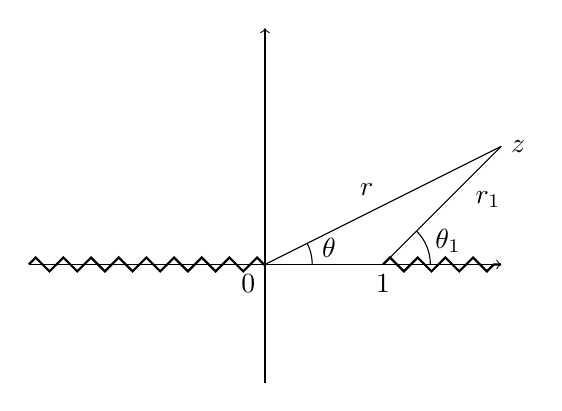
\begin{tikzpicture}[scale=1.5]
    \draw [->] (-2, 0) -- (2, 0);
    \draw [decorate, thick, decoration=zigzag] (-2, 0) -- (0, 0);
    \draw [decorate, thick, decoration=zigzag] (1, 0) -- (2, 0);
    \draw [->] (0, -1) -- (0, 2);
    \node [below] at (1, 0) {$1$};
    \node [anchor = north east] {$0$};
    \node [circle] at (1, 0) {};
    \node [circle] at (0, 0) {};

    \draw (0, 0) -- (2, 1) node [right] {$z$} node [circle] {} node [pos=0.5, anchor = south east] {$r$};
    \draw (1, 0) -- (2, 1) node [pos=0.7, anchor = north west] {$r_1$};

    \draw (0.4, 0) arc(0:26.565:0.4);
    \node at (0.4, 0.14) [right] {$\theta$};

    \draw (1.4, 0) arc (0:45:0.4);
    \node at (1.36, 0.2) [right] {$\theta_1$};
  \end{tikzpicture}
\end{center}
\end{eg}
In fact, we might need fewer branch cuts (less than the number of branch points).
\begin{eg}
$f(z)=\ln\frac{z-1}{z+1}$ has branch points at $\pm 1$. Let $z_1-1=r_1e^{i\theta_1}$ and $z_2+1=r_2e^{i\theta_2}$, then with our choice of branch cut (from 1 to $\infty$ and from $-1$ to $-\infty$), we choose $0\leq\theta_1<2\pi$ and $-\pi<\theta_2\leq\pi$. Then,
$$f(z)=\ln\frac{r_1e^{i\theta_1}}{r_2e^{i\theta_2}}=\ln(r_1/r_2)+i(\theta_1-\theta_2)$$
where we get a single-valued definition of $f(z)$. It is now impossible to wind around either of the two branch points. $f(z)$ is now analytic everywhere except along the branch cuts.\\[5pt]
In that branch cut, we have included the point of $\infty$, which is not necessary since $\infty$ is not a branch point, and thus may allow an infinitely large circle for $z$. An alternative branch cut would be from $-1$ to $+1$, and choose both $\theta_1,\theta_2\in[0,2\pi)$. If $z$ were to wind around just one branch point, then it would cross the branch cut.
\begin{center}
  \begin{tikzpicture}[scale=1.5]
    \draw [->] (-2, 0) -- (2, 0);
    \draw [decorate, thick, decoration=zigzag] (-1, 0) -- (1, 0);
    \draw [->] (0, -1) -- (0, 2);
    \node [below] at (1, 0) {$1$};
    \node [below] at (-1,0) {$-1$};
    \node [circle] at (1, 0) {};
    \node [circle] at (-1, 0) {};

    \draw (-1, 0) -- (2, 1) node [right] {$z$} node [circle] {} node [pos=0.5, anchor = south east] {$r_2$};
    \draw (1, 0) -- (2, 1) node [pos=0.7, anchor = north west] {$r_1$};

    \draw (-0.4, 0) arc(0:26.565:0.4);
    \node at (-0.4, 0.14) [right] {$\theta_2$};

    \draw (1.4, 0) arc (0:45:0.4);
    \node at (1.36, 0.2) [right] {$\theta_1$};
  \end{tikzpicture}
\end{center}
Let's say from above to below, then $\theta_1$ is unchanged at $\pi$, while $\theta_2$ jumps from 0 to $2\pi$, causing a discontinuity in $f(z)$. Nevertheless, we may allow $z$ to wind around both branch cuts together, i.e. for a sufficiently large curve that encircle both branch points exactly once. In that case, $\theta_1,\theta_2$ both suddenly jump from $2\pi$ back to 0 and so $\theta_1-\theta_2$ does not jump.
\end{eg}
\begin{eg}
Similarly, consider $g(z)=(z^2-1)^{1/2}$ with the same branch cut. The single-valued choice of $g(z)$ is $\sqrt{r_1r_2}e^{i(\theta_1+\theta_2)/2}$. When both $\theta_1,\theta_2$ jump by $2\pi$, $\frac{1}{2}(\theta_1+\theta_2)$ jumps by $2\pi$ also, i.e. $e^{2\pi i}=1$, the branch cut prevents either $\theta_1$ or $\theta_2$ jump on its own.
\end{eg}
\newpage
\subsection{Contours and integrals}
\begin{defi}[Curve]
A curve $\gamma(t)$ is a continuous map $\gamma:[0,1]\rightarrow\mathbb{C}$. A closed curve has $\gamma(0)=\gamma(1)$. A simple curve is one that doesn't intersect itself (except at $t=0,1$ if the curve is simple and closed).
\end{defi}
\begin{defi}[Contour]
A contour is a piecewise smooth curve.
\end{defi}
\begin{remarks}\leavevmode
\begin{enumerate}
    \item Given contours $\gamma_1,\gamma_2$ with matching endpoints, i.e. $\gamma_1(1)=\gamma_2(0)$, then $\gamma_1+\gamma_2$ is the two contours joined end-to-end.
    \item The contour $-\gamma$ is $\gamma$ traversed in the opposite direction.
\end{enumerate}
\end{remarks}
\begin{defi}[Contour integral]
The contour integral is defined to be
$$\int_\gamma f(z)dz:=\int_0^1f(\gamma(t))\gamma'(t)dt$$
Alternatively, and equivalently, for a simple contour, we dissect it at points $z_0,z_1,\dots,z_N$ on the contour in that order, where $z_0=\gamma(0)$ and $z_N=\gamma(1)$, and let $\delta_{z_n}=z_{n+1}-z_n$, $n=0,\dots,N-1$. Then
$$\int_\gamma f(z)dz=\lim_{\Delta\rightarrow 0}\sum_{n=0}^{N-1}f(z_n)\delta z_n$$
where $\Delta=\max_{n\in[0,\dots,N-1]}|\delta z_n|$ and as $\Delta\rightarrow 0$, $N\rightarrow\infty$.
\end{defi}
\begin{eg}
The result of a contour integral between two points in $\mathbb{C}$ may depend on the choice of the contour. Consider $I_1=\int_{\gamma_1}\frac{dz}{z}$ and $I_2=\int_{\gamma_2}\frac{dz}{z}$, where in both cases we integrate from $z=-1$ to $+1$ around a unit semi-circle: $\gamma_1$ above and $\gamma_2$ below the real axis, and traversed clockwise and anti-clockwise respectively.
  \begin{center}
    \begin{tikzpicture}[scale=0.75]
      \draw [->] (-3, 0) -- (3, 0);
      \draw [->] (0, -3) -- (0, 3);

      \draw [->-=0.7, red] (-2, 0) arc(180:0:2) node [pos=0.7, anchor = south west] {$\gamma_1$};
      \draw [->-=0.7, blue] (-2, 0) arc(180:360:2) node [pos=0.7, anchor = north west] {$\gamma_2$};

      \draw (0, 0) -- (1.414, 1.414);
      \draw (0.4, 0) arc(0:45:0.4) node [pos=0.8, right] {$\theta$};

      \node [anchor = north west] at (2, 0) {$1$};
      \node [anchor = north east] at (-2, 0) {$-1$};
      \node [circle] at (0, 0) {};
      \node [anchor = north east] {$0$};
    \end{tikzpicture}
  \end{center}
  Substitute $z=e^{i\theta}$, $dz=e^{i\theta}id\theta$, then 
  $$I_1=\int_{\pi}^0\frac{ie^{i\theta}d\theta}{e^{i\theta}}=-i\pi,\quad I_2=\int_{-\pi}^0\frac{ie^{i\theta}d\theta}{e^{i\theta}}d\theta=+i\pi$$
\end{eg}
\begin{prop}[Properties of contour integral]\leavevmode
\begin{enumerate}
    \item $-\int_\gamma f(z)dz=\int_{-\gamma}f(z)dz$;
    \item $\int_{\gamma_1+\gamma_2}f(z)dz=\int_{\gamma_1}f(z)dz+\int_{\gamma_2}f(z)dz$;
    \item If $\gamma$ is a contour from $a$ to $b$ in $\mathbb{C}$, then $\int_\gamma f'(z)dz=f(b)-f(a)$ so long as $f$ is differentiable at every point on $\gamma$. Note, we must not cross a branch cut of $f$;
    \item Integration by substitution and by parts work exactly as for integrals on $\mathbb{R}$;
    \item If $\gamma$ has length $L$ and $|f(z)|\leq M$ on $\gamma_1$, then 
    $$\bigg|\int_\gamma f(z)dz\bigg|\leq\int_\gamma|f(z)||dz|\leq M\int_\gamma |dz|=ML$$
    This is also known as the ML-inequality, or estimation lemma.
\end{enumerate}
\end{prop}
\begin{notation}[Integration on closed contours]
The notation $\oint f(z)dz$ denotes an integral round a closed contour. Doesn't matter where we start. The usual direction for positive sense is anti-clockwise.
\end{notation}
\begin{thm}[Cauchy's theorem]
If $f(z)$ is analytic in a simply-connected domain $D$, then for every simple closed contour $\gamma$ in $D$,
$$\oint_\gamma f(z)dz=0$$
\end{thm}
\begin{proof}
Let $f=u+iv$, then evaluate $\oint_\gamma f(z)dz$:
$$\oint_\gamma(u+iv)(dx+idy)=\oint_\gamma(udx-vdy)+i\oint_{\gamma}(vdx+udy)=\int_S\bigg(-\frac{\partial v}{\partial x}-\frac{\partial u}{\partial y}\bigg)dxdy+i\int_S\bigg(\frac{\partial u}{\partial x}-\frac{\partial v}{\partial y}\bigg)dxdy$$
where $S$ is a region enclosed by $\gamma$, by applying Green's theorem in a plane
$$\oint_{\partial S}(Pdx+Qdy)=\int_S\bigg(\frac{\partial Q}{\partial x}-\frac{\partial P}{\partial y}\bigg)dxdy$$
but both brackets $\frac{\partial u}{\partial x}-\frac{\partial v}{\partial y}$ and $-\frac{\partial v}{\partial x}-\frac{\partial u}{\partial y}$ vanish by CRE, since $f$ is differentiable throughout $S$. The result follows.
\end{proof}
\begin{remarks}
We also require $u$ and $v$ to have continuous partial derivatives in $S$ in order for Green's theorem to be true. There is a completely different proof available if we do not wish to make assumptions on $u$ and $v$.
\end{remarks}
\begin{thm}[Deformation theorem]
Suppose $\gamma_1,\gamma_2$ are two contours from $a$ to $b$, and that $f$ is analytic on and between them. Then
$$\int_{\gamma_1}f(z)dz=\int_{\gamma_2}f(z)dz$$
\end{thm}
\begin{proof}
Suppose first that $\gamma_1,\gamma_2$ do not cross. Then $\gamma_1-\gamma_2$ is a simple closed contour, so $\oint_{\gamma_1-\gamma_2}f(z)dz=0$ by Cauchy's theorem and the result follows.\\[5pt]
If $\gamma_1$ and $\gamma_2$ do cross, then dissect them at each crossing point, and apply the technique above to each section. Done.
\end{proof}
\begin{remarks}\leavevmode
\begin{enumerate}
    \item Essentially, if $f$ has no singularities, $\int_a^bf(z)dz$ does not depend on the choice of contour.
    \item Another way of thinking about path-independence and indeed Cauchy's theorem itself, is to consider $\int f(z)dz$ as a path integral in $\mathbb{R}^2$. Then
    $$f(z)dz=(u+iv)(dx+idy)=(u+iv)dx+(-v+iu)dy$$
    is an exact differential. Hence, by CRE,
    $$\frac{\partial}{\partial y}(u+iv)=\frac{\partial}{\partial x}(-v+iu)$$
    \item The deformation theorem also applies to closed contours. Let $\times$ denote a singularity in $\mathbb{C}$.

\begin{center}
  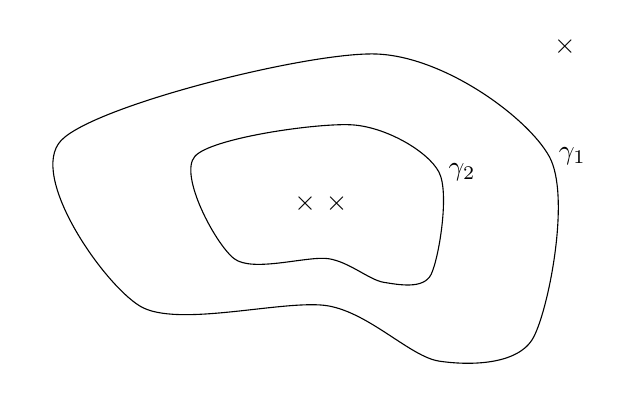
\begin{tikzpicture}
    \draw [->] plot [smooth cycle] coordinates {(-1.2, -0.7) (0, -0.7) (0.7, -1) (1.3, -0.9) (1.4, 0.4) (0.3, 1) (-1.7, 0.6)};
    \draw [->] plot [smooth cycle] coordinates {(-2.4, -1.3) (0, -1.3) (1.4, -2) (2.6, -1.7) (2.8, 0.6) (0.6, 1.9) (-3.4, 0.8)};

    \node [right] at (1.4, 0.4) {$\gamma_2$};
    \node [right] at (2.8, 0.6) {$\gamma_1$};
    \node at (0.1, 0) {$\times$};
    \node at (-0.3, 0) {$\times$};
    \node at (3, 2) {$\times$};
  \end{tikzpicture}
\end{center}
Suppose $\gamma_1$ is a closed contour that can be continuously deformed into another, $\gamma_2$, inside it, and there are no singularities in the region between them. Essentially, consider the contour $\gamma$ shown:
\begin{center}
  \begin{tikzpicture}
   \draw [-<-=0.4, -<-=0.8] plot [smooth cycle] coordinates {(-1.2, -0.7) (0, -0.7) (0.7, -1) (1.3, -0.9) (1.4, 0.4) (0.3, 1) (-1.7, 0.6)};
    \draw [->-=0.3, ->-=0.7, ->-=0.9] plot [smooth cycle] coordinates {(-2.4, -1.3) (0, -1.3) (1.4, -2) (2.6, -1.7) (2.8, 0.6) (0.6, 1.9) (-3.4, 0.8)};

    \node [right] at (2.8, 0.6) {$\gamma$};
    \node at (0.1, 0) {$\times$};
    \node at (-0.3, 0) {$\times$};
    \node at (3, 2) {$\times$};

    \draw [white, very thick] (2.4, 1.07) -- (2.1, 1.3);
    \draw [white, line width=0.5cm] (1.16, 0.65) -- (1.4, 0.4);
    \draw [->-=0.7] (2.4, 1.07) -- (1.4, 0.4);
    \draw [-<-=0.4] (2.1, 1.3) -- (1.16, 0.65);
  \end{tikzpicture}
\end{center}
\end{enumerate}
Then by Cauchy's theorem,
$$\oint_\gamma f(z)dz=0$$
Now let the distance between the two `cross-cuts' tend to 0, then those contributions cancel out and, in this limit
$$\oint_{\gamma_1}f(z)dz-\oint_{\gamma_2}f(z)dz=0$$

\end{remarks}

\subsection{Residues}
\begin{defi}[Residue]
The residue of $f$ at $z_0$ is the coefficient of $a_{-1}$ of its Laurent series.
\end{defi}
\begin{notation}
We denote the residue as $\res_{z=z_0}f(z)$.
\end{notation}
\begin{prop}\leavevmode
\begin{enumerate}
    \item At a simple pole, the residue is $\res_{z=z_0}f(z)=\lim_{z\rightarrow z_0}((z-z_0)f(z))$.
    \item More generally, at a pole of order $N$, the residue is $$\res_{z=z_0}f(z)=\lim_{z\rightarrow z_0}\bigg[\frac{1}{(N-1)!}\frac{d^{N-1}}{dz^{N-1}}((z-z_0)^Nf(z)\bigg]$$
\end{enumerate}
\end{prop}
\begin{proof}
At a simple pole, $a_n=0$ $\forall n<-1$, so
$$\lim_{z\rightarrow z_0}\bigg[(z-z_0)\bigg(\frac{a_{-1}}{z-z_0}+a_0+a_1(z-z_0)+\dots\bigg)\bigg]=a_{-1}$$
For the more general case, we can prove it in a similar manner.
\end{proof}
In practice, a variety of techniques can be used to evaluate residues, i.e. no single technique is optimal for all situations. Sometimes, L'Hopital rule is helpful.
\begin{eg}[Calculating residues]\leavevmode
\begin{enumerate}
    \item $\frac{e^z}{z^3}$ at $z=0$: Laurent series about $z=0$ is
    $$z^{-3}+z^{-2}+\frac{1}{2}z^{-1}+\frac{1}{3!}+\dots$$
    so residue is $0.5$. Alternatively, $f$ has a pole of order 3 at $z=0$, so
    $$\res_{z=0} f(z)=\lim_{z\rightarrow0}\bigg\{\frac{1}{2!}\frac{d^2}{dz^2}(z^3f(z))\bigg\}=\frac{1}{2}\lim_{z\rightarrow0}\frac{d^2}{dz^2}e^z=\frac{1}{2}$$
    \item $\frac{e^z}{z^2-1}$ at $z=1$: Laurent series about $z=1$ is
    $$\frac{e}{2}\bigg(\frac{1}{z-1}+\frac{1}{2}+\dots\bigg)$$
    so residue is $\frac{1}{2}e$. Alternatively,
    $$\res_{z=1}g(z)=\lim_{z\rightarrow1}\frac{(z-1)e^z}{z^2-1}=\lim_{z\rightarrow1}\frac{e^2}{z+1}=\frac{1}{2}e$$
    \item $\frac{1}{z^8-w^8}$ at $z=w$: we have 8 simple poles $z=we^{n\pi i/4}$ with $n=0,1,\dots,7$. There are two ways to evaluate $\res_{z=w}\frac{1}{z^8-w^8}=\lim_{z\rightarrow w}\frac{z-w}{z^8-w^8}$: either brute force
    $$\frac{1}{(w^2-(we^{i\pi/4})^2)(2w^2)(w^2-(we^{i3\pi/4})^2)(2w)}=\frac{1}{(1-i)2(1+i)2w^7}=\frac{1}{8w^7}$$
    or just L'Hopital rule:
    $$\lim_{z\rightarrow w}\frac{z-w}{z^8-w^8}=\lim_{z\rightarrow w}\frac{1}{8z^7}=\frac{1}{8w^7}$$
    \item $\sech(\pi z)$ at $z=(n+0.5)i$: simple poles $\forall n\in\mathbb{Z}$ (since they are simple zeros for $\cosh (\pi z)$. Use L'Hopital rule to evaluate 
    $\res_{z=(n+0.5)i}\sech(\pi z)$
    $$\lim_{z\rightarrow(n+0.5)i}\frac{z-(n+0.5)i}{\cosh(\pi z)}=\lim_{z\rightarrow(n+0.5)i}\frac{1}{\pi\sinh(\pi z)}=\frac{1}{\pi i\sinh(n+0.5)\pi}=\frac{-i(-1)^n}{\pi}$$
    \item $\frac{1}{\sinh^3z}$ at $z=\pi i$: zero of order 3. The Laurent series about $z=\pi i$ is 
    $$\sinh^3z=-(z-\pi i)^3-\frac{1}{2}(z-\pi i)^5-\dots$$
    $$\implies\frac{1}{\sinh^3z}=-(z-\pi i)^{-3}(1+0.5(z-\pi i)^2+\dots)^{-1}=-(z-\pi i)^{-3}+0.5(z-\pi i)^{-1}+\dots$$
    Hence the residue is $\res_{z=\pi i}\frac{1}{\sinh^3 z}=0.5$.
\end{enumerate}
\end{eg}
\begin{thm}[Residue theorem]
Suppose $f$ is analytic in a simply-connected domain except at a finite number of isolated singularities $\{z_1,\dots,z_n\}$. Suppose a simple closed contour $\gamma$ encircles the origin anticlockwise, then
$$\oint_\gamma f(z)dz=2\pi i\sum_{k=1}^n\res_{z=z_k}f(z)$$
\begin{center}
  \begin{tikzpicture}
    \draw [->-=0.3, ->-=0.7, ->-=0.9] plot [smooth cycle] coordinates {(-2.4, -1.3) (0, -1.3) (1.4, -2) (2.6, -1.7) (2.8, 0.6) (0.6, 1.9) (-3.4, 0.8)};
    \node [circle] (z1) at (1.8, 0) {$\times$};
    \node [right] at (z1) {$z_1$};
    \node [circle] (z2) at (0, 1) {$\times$};
    \node [right] at (z2) {$z_2$};
    \node [circle] (z3) at (-2, -0.5) {$\times$};
    \node [right] at (z3) {$z_3$};
    \node at (3, 1) {$\gamma$};
  \end{tikzpicture}
\end{center}
\end{thm}
\begin{proof}
Consider $\hat{\gamma}$ shown, consisting of small clockwise circles $\gamma_1,\dots,\gamma_n$ around each singularity, cross-cuts which cancel in the limit as they approach each other in pairs, and the large outer curve (which is $\gamma$ in this limit).
 \begin{center}
    \begin{tikzpicture}
      \draw [->-=0.3, ->-=0.7, ->-=0.9] plot [smooth cycle] coordinates {(-2.4, -1.3) (0, -1.3) (1.4, -2) (2.6, -1.7) (2.8, 0.6) (0.6, 1.9) (-3.4, 0.8)};
      \node [circle] (z1) at (1.8, 0) {$\times$};
      \node [circle] (z2) at (0, 1) {$\times$};
      \node [circle] (z3) at (-2, -0.5) {$\times$};

      \node at (3, 1) {$\hat{\gamma}$};
      \draw [-<-=0.5] (z1) circle [radius=0.5];
      \draw [-<-=0.75](z2) circle [radius=0.5];
      \draw [-<-=0.75] (z3) circle [radius=0.5];

      \draw [white, line width=0.5cm] (2.91, 0.1) -- (2.92, -0.1);
      \draw [white, line width=0.5cm] (2.29, 0.1) -- (2.29, -0.1);
      \draw (2.29, 0.1) -- (2.91, 0.1);
      \draw (2.29, -0.1) -- (2.92, -0.1);

      \draw [white, line width=0.5cm] (0.1, 1.49) -- (-0.1, 1.49);
      \draw [white, line width=0.5cm] (0.1, 1.86) -- (-0.1, 1.84);
      \draw (0.1, 1.49) -- (0.1, 1.86);
      \draw (-0.1, 1.49) -- (-0.1, 1.84);

      \draw [white, line width=0.5cm] (-3.05, -0.6) -- (-3.18, -0.4);
      \draw [white, line width=0.5cm] (-2.49, -0.6) -- (-2.49, -0.4);
      \draw (-2.49, -0.6) -- (-3.05, -0.6);
      \draw (-2.49, -0.4) -- (-3.18, -0.4);

      \node [right] at (z1) {$z_1$};
      \node [right] at (z2) {$z_2$};
      \node [right] at (z3) {$z_3$};
    \end{tikzpicture}
  \end{center}
Since $\hat{\gamma}$ encircles no singularities, then by Cauchy's theorem $\oint_{\hat{\gamma}}f(z)dz=0$. Hence, in the limit when the cross-cuts cancel, we have
$$\oint_\gamma f(z)dz+\sum_{k=1}^n\oint_{\gamma_k}f(z)dz=\oint_{\hat{\gamma}}f(z)dz=0$$
But about each singularity $z_k$, there is a Laurent series valid locally in some annulus, so we have
$$\oint_{\gamma_k}f(z)dz=-2\pi i\res_{z=z_k}f(z)$$
where we used minus sign since $\gamma_k$ is a clockwise contour encircling the singularity. The result follows. 
\end{proof}
\begin{thm}[Cauchy's integral formula]
Suppose $f$ is analytic in a simply-connected domain $D$ and $z\in D$, then for any simple closed contour $\gamma$ in $D$ encircling $z$ anti-clockwise,
$$f(z)=\frac{1}{2\pi i}\oint_{\gamma}\frac{f(w)}{w-z}dw$$
\end{thm}
\begin{proof}
 The only singularity of the integrand is at $w=z$, and is a simple pole (since $f$ is analytic there). Hence, using the residue theorem and the formula in Section 4.1, the integral equals 
$$2\pi i\res_{w=z}\frac{f(w)}{w-z}=2\pi i\lim_{w\rightarrow z}f(w)=2\pi if(z)$$
Result follows.
\end{proof}
\begin{remarks}\leavevmode
\begin{enumerate}
    \item If $z$ lies outside $\gamma$, RHS is 0 by Cauchy's theorem.
    \item If we know $f$ on $\gamma$, then we know it at all points within $\gamma$. Another way of looking at this is to write $f=u+iv$, with $u,v$ harmonic, and are both specified on $\gamma$. Then we have Laplace's equation for $u$ and $v$ with Dirichlet b.c.s, which has a unique solution inside $\gamma$. Cauchy's formula thus gives us a way of calculating that solution explicitly.
    \item Normally, Cauchy's integral formula is proved before the residue theorem, because it's needed to prove the existence of Laurent series.
\end{enumerate}
\end{remarks}
\begin{cor}
$$f^{(n)}(z)=\frac{n!}{2\pi i}\oint_\gamma\frac{f(w)}{(w-z)^{n+1}}dw$$
\end{cor}
\begin{proof}
Differentiating Cauchy's formula $n$ times give the result. Differentiation under the integral sign is valid because the integrand, both before and after, is a continuous function of $w$ and $z$. Hence, at any point where $f$ is analytic, all its derivatives exist, so it is differentiable infinitely many times.
\end{proof}
\begin{cor}[Liouville's theorem]
Any bounded entire function is constant.
\end{cor}
\begin{proof}
Suppose $|f(z)|\leq M$ $\forall z$ and consider a circle of arbitrary radius $R$, centred at a given $z\in\mathbb{C}$, then
$$f'(z)=\frac{1}{2\pi i}\oint_{|w-z|=R}\frac{f(w)dw}{(w-z)^2}\implies|f'(z)|\leq\frac{1}{2\pi}2\pi R\frac{M}{R^2}\implies\lim_{R\rightarrow\infty}|f'(z)|=0$$
where we used ML inequality. Hence, $f'(z)=0$ $\forall z\in\mathbb{C}$, so $f$ is constant.
\end{proof}
\begin{cor}[Maximum moduli principle]
If $f(z)$ is analytic within a bounded domain and on its boundary, then $|f(z)|$ attains its maximum on the boundary.
\end{cor}
\begin{proof}
 Let $0 < \rho < r$. Applying the Cauchy integral formula for $w=z+\rho e^{2\pi i\theta}$, we get
  \begin{align*}
    |f(z)| &= \left|\frac{1}{2\pi i}\int_{|w-z|=\rho} \frac{f(w)}{w - z}\;d w\right|\\
    &= \left|\int_0^1 f(z + \rho e^{2 \pi i \theta})\;d \theta\right|\\
    &\leq f(z).
  \end{align*}
 So we must have equality throughout. So $|f(w)|$ is constant on the circle $|z - w| = \rho$, and is equal to $f(z)$. Since this is true for all $\rho \in (0, r)$, it follows that $|f|$ is constant on this circular domain. Then the CRE entail that $f$ must be constant.
\end{proof}
\subsection{Applications of the residue theorem}
To illustrate the technique known as the 'calculus of residue', consider the following example:
\begin{eg}
Evaluate
$$I=\int_0^\infty\frac{dx}{1+x^2}$$
Consider $\oint_\gamma\frac{dz}{1+z^2}$, where $\gamma$ is the contour consisting of $\gamma_0$ followed by $\gamma_R$: from $-R$ to $R$ along the real axis, then returning to $-R$ via a semicircle of radius $R$ in the upper half plane. This is known as \textbf{closing in the upper half-plane} or closing above.
\begin{center}
    \begin{tikzpicture}
      \draw [->] (-3, 0) -- (3, 0);
      \draw [->] (0, -1) -- (0, 3);

      \draw [black, thick, ->-=0.3, ->-=0.8] (-2, 0) -- (2, 0) node [pos=0.3, below] {$\gamma_0$} arc(0:180:2) node [pos=0.3, right] {$\gamma_R$};

      \node [below] at (-2, 0) {$-R$};
      \node [below] at (2, 0) {$R$};

      \node at (0, 1) {$\times$};
      \node [right] at (0, 1) {$i$};
    \end{tikzpicture}
  \end{center}
Now $\frac{1}{1+z^2}=\frac{1}{(z+i)(z-i)}$, so the only singularity enclosed by $\gamma$ is a simple pole at $z=i$, whose residue is $\lim_{z\rightarrow i}\frac{z-i}{z^2+1}=\frac{1}{2i}$. Hence,
$$\oint_{\gamma_0}\frac{dz}{1+z^2}+\oint_{\gamma_R}\frac{dz}{1+z^2}=\oint_{\gamma}\frac{dz}{1+z^2}=2\pi i\res_{z=i}\frac{1}{1+z^2}=\pi$$
But 
$$\oint_{\gamma_0}\frac{dz}{1+z^2}=\int{-R}^R\frac{dx}{1+x^2}\rightarrow 2I,\text{  as  }R\rightarrow\infty$$
Also, we can justify $\int_{\gamma_R}\frac{dz}{1+z^2}\rightarrow 0$ as $R\rightarrow\infty$. Doing this formally:
$$|1+z^2|\geq|1-|z|^2|=|1-R^2|=R^2-1$$
by triangle inequality and where $R$ is large. So, $|\frac{1}{1+z^2}|\leq\frac{1}{R^2-1}$ and hence by the ML inequality,
$$\bigg|\int_{\gamma_R}\frac{dz}{1+z^2}\bigg|\leq\frac{\pi R}{R^2-1}\rightarrow 0,\text{  as  }R\rightarrow\infty$$
Or informally: for $z\in\gamma_R$, we use the ML inequality:
$$\bigg|\frac{1}{1+z^2}\bigg|=O(R^{-2})\implies\bigg|\int_{\gamma_R}\frac{dz}{1+z^2}\bigg|\leq\pi R~O(R^{-2})=O(R^{-1})\rightarrow 0,\text{ as }R\rightarrow\infty$$
as we will see later, the informal argument is easier for more difficult integrals.
\end{eg}
\begin{eg}\leavevmode
\begin{enumerate}
    \item Evaluate
    $$I=\int_0^\infty\frac{dx}{(x^2+a^2)^2}$$
    where $a>0$ is a real constant. Consider $\oint_\gamma\frac{dz}{(z^2+a^2)^2}$, with $\gamma$ real axis closed in the upper half-plane (as before). The only singularity within $\gamma$ is a pole of order 2 at $z=ia$, at which residue is
    $$\res_{z=ia}\frac{1}{(z^2+a^2)^2}=\lim_{z\rightarrow ia}\frac{d}{dz}\frac{(z-ia)^2}{(z+ia)^2(z-ia)^2}=\lim_{z\rightarrow ia}\frac{-2}{(z+ia)^3}=\frac{-2}{-8ia^3}=-\frac{1}{4}ia^{-3}$$
    The integral round $\gamma_R$ will vanish as $R\rightarrow\infty$, since by the ML inequality,
    $$\bigg|\int_{\gamma_R}\frac{dz}{(z^2+a^2)^2}\bigg|\leq\pi R ~O(R^{-4})=O(R^{-3})$$
    Hence, $2I=2\pi i(-0.25 ia^{-3})\implies I=\frac{\pi}{4a^3}$.
    \item For $I=\int_0^\infty\frac{dx}{1+x^4}$, use the same contour $\gamma$ again. There are simple poles at $e^{\pm i\pi/4}$, $e^{\pm 3\pi i/4}$, but only the first two are enclosed, with residues $-\frac{1}{4}e^{i\pi/4}$ and $+\frac{1}{4}e^{-i\pi/4}$. The integral round the semicircle is bounded by $\pi R~O(R^{-4})\rightarrow 0$ as $R\rightarrow\infty$. Hence,
    $$2I=2\pi i(-0.25e^{\pi i/4}+0.25e^{-\pi i/4})\implies I=\frac{\pi}{2\sqrt{2}}$$
    Alternatively could use a quarter circle contour to enclose one pole only, say $e^{i\pi/4}$.
\end{enumerate}
\end{eg}
For trigonometric integrals of the form
$$\int_0^{2\pi}f(\sin\theta,\cos\theta)d\theta$$
substitute $z=e^{i\theta}\implies dz=izd\theta$, and $\cos\theta=\frac{1}{2}(z+z^{-1})$ and $\sin\theta=\frac{1}{2i}(z-z^{-1})$ to obtain a closed contour integral. 
\begin{eg}
Evaluate
$$I=\int_0^{2\pi}\frac{d\theta}{a+\cos\theta},\quad a>1$$
so that the integrand is always finite. Substitute $z=e^{i\theta}$,
$$I=\oint_{\gamma}\frac{(iz)^{-1}dz}{a+0.5(z+z^{-1})}=-2i\oint_\gamma\frac{dz}{z^2+2az+1}$$
where the integrand has poles $z_\pm=-a\pm\sqrt{a^2-1}$, both on the real axis. Since $a-1<\sqrt{a^2-1}<a$, then $-1<z_+<0$, i.e. $z_+$ is inside the unit circle. 
 \begin{center}
    \begin{tikzpicture}
      \draw [->] (-3, 0) -- (3, 0);
      \draw [->] (0, -3) -- (0, 3);
      \draw [black, thick, ->-=0.2,->-=0.7] circle [radius=1.8];
      \node [right] at (1.2726, 1.2726) {$\gamma$};

      \node (z-) at (-2.5, 0) {$\times$};
      \node [below] at (z-) {$z_-$};

      \node (z+) at (-1.2, 0) {$\times$};
      \node [below] at (z+) {$z_+$};
    \end{tikzpicture}
  \end{center}

The residue at $z=z_+$ is
$$\res_{z=z_+}\frac{1}{z^2+2az+1}=\lim_{z\rightarrow z_+}\frac{z-z_+}{z^2+2az+1}=\frac{1}{z_+-z_-}=\frac{1}{2\sqrt{a^2-1}}$$
Hence, $I=-2i\frac{2\pi i}{2\sqrt{a^2-1}}=\frac{2\pi}{\sqrt{a^2-1}}$.
\end{eg}
\begin{eg}[Integration around a branch cut]
Evaluate
$$I=\int_0^\infty\frac{x^\alpha}{1+\sqrt{2}x+x^2}dx,\quad -1<\alpha<1$$
so that the integral converges. Need branch cut for $z^\alpha$. Take this along the positive real axis, $z^\alpha:=r^\alpha e^{i\alpha\theta}$, where $0\leq\theta<2\pi$. Consider
$$\oint_\gamma\frac{z^\alpha}{1+\sqrt{2}z+z^2}dz$$
where $\gamma$ is a keyhole contour, consisting of a large circle $\gamma_R$ of radius $R$, a small circle $\gamma_\varepsilon$ of radius $\varepsilon$ (to avoid singularity of $z^\alpha$ at $z=0$) and two lines just above and below the branch cut.
   \begin{center}
    \begin{tikzpicture}
      \draw [->] (-3, 0) -- (3, 0);
      \draw [->] (0, -3) -- (0, 3);
      \draw [thick,decorate, decoration=zigzag] (0, 0) -- (3, 0);

      \draw [black, thick, ->-=0.1, ->-=0.45, ->-=0.75, ->-=0.84, ->-=0.95] (1.977, 0.3) arc(8.63:351.37:2) node [pos=0.15, anchor = south west] {$C_R$} -- (0.4, -0.3) arc(323.13:36.87:0.5) node [pos=0.7, left] {$C_\varepsilon$} -- cycle;

      \node [circle] at (0, 0) {};

      \node at (-1, -1) {$\times$};
      \node [right] at (-1, -1) {$e^{5\pi i/4}$};
      \node at (-1, 1) {$\times$};
      \node [right] at (-1, 1) {$e^{3\pi i/4}$};
    \end{tikzpicture}
  \end{center}
  The contributions from $\gamma_R$ and $\gamma_\varepsilon$ respectively are
  $$2\pi R~O(R^{\alpha-2})=O(R^{\alpha-1})\rightarrow 0,\text{   as }R\rightarrow\infty$$
  $$2\pi\varepsilon ~O(\varepsilon^{\alpha})=O(\varepsilon^{\alpha+1})\rightarrow 0,\text{   as }\varepsilon\rightarrow0$$
  where $\alpha<1$ and $\alpha>-1$ respectively. Above and below the branch cut respectively:
  $$\int_{\varepsilon}^R\frac{x^\alpha}{1+\sqrt{2}x+x^2}dx\rightarrow I,\text{  as  }\varepsilon\rightarrow0,R\rightarrow\infty$$
  $$\int_R^{\varepsilon}\frac{x^\alpha e^{2\pi i\alpha}}{1+\sqrt{2}x+x^2}dx\rightarrow-e^{2\pi i\alpha}I,\text{  as  }\varepsilon\rightarrow0,R\rightarrow\infty$$
  Thus,
  $$\oint_\gamma\frac{z^\alpha}{1+\sqrt{2}z+z^2}dz\rightarrow(1-e^{2\pi i\alpha})I,\text{  as }\varepsilon\rightarrow0,R\rightarrow\infty$$
  The integrand is equal to $\frac{z^\alpha}{(z-e^{3\pi i/4})(z-e^{i5\pi/4})}$. The poles inside $\gamma$ have residues
  $$\res_{z=e^{3\pi i/4}}\frac{z^\alpha}{(z-e^{3\pi i/4})(z-e^{i5\pi/4})}=\frac{e^{3\pi i\alpha/4}}{\sqrt{2}i}$$
  $$\res_{z=e^{5\pi i/4}}\frac{z^\alpha}{(z-e^{3\pi i/4})(z-e^{i5\pi/4})}=\frac{e^{5\pi i\alpha/4}}{-\sqrt{2}i}$$
  Note that it is not wise to write the location of the pole $e^{i5\pi/4}$ as $e^{-i3\pi/4}$, since this is inconsistent with the chosen branch for $z^\alpha$. Hence, with $\varepsilon\rightarrow0$, $R\rightarrow\infty$:
  $$(1-e^{2\pi i\alpha})I=2\pi i\bigg(\frac{e^{3\alpha i\pi/4}}{\sqrt{2}i}+\frac{e^{5\alpha i\pi/4}}{-\sqrt{2}i}\bigg)\implies I=\sqrt{2}\pi\frac{\sin(\alpha\pi/4)}{\sin(\alpha\pi)}$$
\end{eg}
\begin{lemma}
If $z=x+iy$, then
$$|\sinh y|\leq f(z)\leq\cosh y$$
where $f(z)=|\cos z|,|\sin z|$, and
$$|\sinh x|\leq g(z)\leq\cosh x$$
where $g(z)=|\sinh z|,|\cosh z|$. Hence, as $y\rightarrow\pm\infty$, $f(z)\sim\frac{1}{2}e^{|y|}$, while as $x\rightarrow\pm\infty$, $g(z)\sim\frac{1}{2}e^{|x|}$.
\end{lemma}
\begin{proof}
For $\sin z$, note that $|e^{iz}|=|e^{ix}e^{-y}|=e^{-y}$. Apply the triangle inequality:
$$||z_1|-|z_2||\leq|z_1-z_2|\leq|z_1|+|z_2|$$
with $z_1=e^{iz}$ and $z_2=e^{-iz}$. Similar proof for $\cos z$, $\sinh z$ and $\cosh z$.
\end{proof}
\begin{eg}[Using rectangular contours]
Evaluate
$$I=\int_{-\infty}^\infty\frac{e^{\alpha x}}{\cosh x}dx,\quad \alpha\in\mathbb{R},\alpha\in(-1,1)$$
Use a rectangular contour as shown:
  \begin{center}
    \begin{tikzpicture}
      \draw [->] (-3, 0) -- (3, 0);
      \draw [->] (0, -1) -- (0, 3);

      \draw [black, thick, ->-=0.3, ->-=0.4,->-=0.8,->-=0.95] (-2, 0) node [below] {$-R$} -- (2, 0) node [pos=0.7, below] {$\gamma_0$} node [below] {$R$} -- (2, 1.5) node [pos=0.5, right] {$\gamma_R^+$} -- (-2, 1.5) node [pos=0.3, above] {$\gamma_1$} -- (-2, 0) node [pos=0.5, left] {$\gamma_R^-$};

      \node at (0, 0.75) {$\times$};
      \node [left] at (0, 0.75) {$\frac{\pi i}{2}$};

      \node [circle] at (0, 1.5) {};
      \node [anchor = south east] at (0, 1.5) {$\pi i$};
    \end{tikzpicture}
  \end{center}
 We see that
 $$\int_{\gamma_0}\frac{e^{\alpha z}}{\cosh z}dz\rightarrow I,\text{ as }R\rightarrow\infty$$
 $$\int_{\gamma_1}\frac{e^{\alpha z}}{\cosh z}dz=\int_{R}^{-R}\frac{e^{\alpha(x+\pi i)}}{\cosh(x+\pi i)}dx=e^{\alpha\pi i}\int_R^{-R}\frac{e^{\alpha x}}{-\cosh x}dx\rightarrow e^{\alpha\pi i}I$$
 On $\gamma_R$, $z=R+iy\implies|\cosh z|\sim\frac{1}{2}e^R$ from Lemma 12.1. Also $|e^{\alpha z}|=e^{\alpha R}$, hence
 $$\bigg|\frac{e^{\alpha z}}{\cosh z}\bigg|=O(e^{(\alpha-1)R})\rightarrow 0,\text{  as }R\rightarrow\infty$$
 so $\int_{\gamma_R}\rightarrow 0$. Similar for $\int_{\gamma_{-R}}$. The only singularity enclosed is at $+\frac{\pi i}{2}$ with residue
 $$\res_{z=\pi i/2}\frac{e^{\alpha z}}{\cosh z}=\frac{e^{\alpha\pi i/2}}{\sinh(\pi i/2)}=-ie^{\alpha\pi i/2}$$
 Hence,
 $$I(1+e^{\alpha\pi i})=2\pi i(-ie^{\alpha\pi i/2})\implies I=\pi\sec\frac{\alpha\pi}{2}$$
\end{eg}
It is possible to use contour integration to sum infinite series. Traditionally, this is done using $\cot z$ and a large square contour that has been chosen carefully to avoid all singularities. 
\begin{eg}[Summation of series using square contour]
Evaluate $\sum_{n=1}^\infty\frac{1}{n^2}$ by integrating suitable function around a square contour. Consider
$$\oint_\gamma\frac{\cot\pi z}{z^2}dz$$
where $\gamma$ is the square contour with vertices at $(N+0.5)(\pm1\pm i)$. $N$ is large, so $\gamma$ avoids all singularities. The integrand have simple poles at $z=n\in\mathbb{Z}$, $n\neq0$ with residues $\frac{1}{n^2\pi}$. There is also a triple pole at $z=0$, i.e.
$$\frac{\cot \pi z}{z^2}=\frac{1}{z^2(\pi z+(\pi^3z^3/3)+\dots)}=\frac{1}{\pi z^3}\bigg(1-\frac{1}{3}\pi^2z^2+\dots\bigg)$$
with residue $-\frac{1}{3}\pi$. 
\begin{center}
    \begin{tikzpicture}
      \draw [->] (-3, 0) -- (3, 0);
      \draw [->] (0, -3) -- (0, 3);

      \foreach \x in {-2.5,-2,...,2.5} {
        \node at (\x, 0) {$\times$};
      }

      \draw [black, thick, -<-=0.1,-<-=0.3, -<-=0.7,-<-=0.9] (1.75, 1.75) rectangle (-1.75, -1.75);

      \node [anchor = south west] at (0, 1.75) {$(N + \frac{1}{2})i$};
      \node [anchor = north west] at (0, -1.75) {$-(N + \frac{1}{2})i$};
      \node [anchor = south west] at (1.75, 0) {$N + \frac{1}{2}$};
      \node [anchor = south east] at (-1.75, 0) {$-(N + \frac{1}{2})$};

      \node [circle] at (0, 1.75) {};
      \node [circle] at (0, -1.75) {};
      \node [circle] at (1.75, 0) {};
      \node [circle] at (-1.75, 0) {};
    \end{tikzpicture}
  \end{center}

As $N\rightarrow\infty$, the integrals along the sides vanish (as we will justify below), so by the Residue theorem:
$$2\pi i\bigg(2\sum_{n=1}^N\frac{1}{n^2\pi}-\frac{\pi}{3}\bigg)\rightarrow 0\implies\sum_{n=1}^\infty\frac{1}{n^2}=\frac{\pi^2}{6}$$
To demonstrate the behaviour of the integrals along the sides, show that on $\gamma$, $\cot\pi z$ is bounded by constant $M$ that does not depend on $N$. By the ML inequality:
$$\bigg|\oint_{\gamma}\frac{\cot\pi z}{z^2}dz\bigg|\leq4(2N+1)\frac{M}{(N+0.5)^2}\rightarrow 0,\text{ as }N\rightarrow\infty$$
Consider the RHS, $z=N+0.5+iy$:
$$|\cot\pi z|=\frac{|\cos((N+0.5)\pi+i\pi y)|}{|\sin((N+0.5)\pi+i\pi y)|}=|-\tan i\pi y|=|\tanh\pi y|\leq1$$
Similar for LHS. Consider top side, $z=(N+0.5)i+x$:
$$|\cot\pi z|=\frac{|\cos\pi z|}{|\sin\pi z|}\leq\frac{\cosh(N+0.5)\pi}{|\sinh(N+0.5)\pi|}=\coth(N+0.5)\pi$$
where by Lemma 12.1, $|\sin z|\geq|\sinh\text{Im}[z]|$ and $|\cos z|\leq\cosh\text{Im}[z]$. Now $\coth\theta\rightarrow 1$ as $\theta\rightarrow\infty$, so in particular it is bounded (by say, 2) for sufficiently large $\theta$; hence $\cot\pi z$ is bounded by 2 for sufficiently large $N$. Similar for bottom side. Here, we may choose $M=2$ for sufficiently large $N$.
\end{eg}
\newpage
\section{Transform methods}
{\small\textcolor{darkblue}{Fourier inversion by contour integration. Examples of simple linear differential equations, including diffusion equation.}\hfill\textbf{[2]}}
\subsection{Jordan's lemma}
\begin{lemma}[Jordan's Lemma]
Suppose $f$ is analytic function, except for a finite number of singularities, and $f(z)\rightarrow 0$ as $|z|\rightarrow\infty$. Then for any real constant $\lambda>0$,
$$\int_{\gamma_R}f(z)e^{i\lambda z}dz\rightarrow 0,~\text{ as }R\rightarrow\infty$$
where $\gamma_R$ is a semicircle of radius $R$ in the upper half-plane. For $\lambda<0$, same conclusion holds for semicircle $\gamma_R$ in the lower half-plane.
\begin{center}
    \begin{tikzpicture}
      \draw [->] (-3, 0) -- (3, 0);
      \draw [->] (0, -3) -- (0, 3);

      \draw [red, thick, ->-=0.3, ->-=0.8] (2, 0) arc(0:180:2) node [pos=0.3, right] {$\gamma_R$};
      \draw [blue, thick, ->-=0.3, ->-=0.8] (2, 0) arc(0:-180:2) node [pos=0.3, right] {$\gamma_R'$};

      \node [anchor = north east] at (-2, 0) {$-R$};
      \node [anchor = north west] at (2, 0) {$R$};
      \node [circle] at (-2, 0) {};
      \node [circle] at (2, 0) {};

      \node at (1, 1) {$\times$};
      \node at (-1, -0.5) {$\times$};
      \node at (-0.3, 0.6) {$\times$};
    \end{tikzpicture}
  \end{center}
\end{lemma}
Such integrals are frequently in applications, particularly with Fourier transforms (see Chapter 5).
\begin{remarks}\leavevmode
\begin{enumerate}
    \item Result easy to show in `straightforward cases' when $f(z)$ decays more rapidly than $\frac{1}{z}$ as $|z|\rightarrow\infty$. Then $|f(z)|=o(1/R)$ on $\gamma_R$, and since $|e^{i\lambda z}|=e^{-\lambda\text{Im}[z]}\leq 1$ on $\gamma_R$, we have
    $$\bigg|\int_{\gamma_R}f(z)e^{i\lambda z}dz\bigg|\leq\pi R~o(1/R)\rightarrow 0,~\text{ as }R\rightarrow\infty$$
    \item But in `sensitive cases', when $f$ decays less rapidly than $o(1/z)$, the proof relies on the fact that for $\theta\in[0,\pi/2]$, $\sin\theta\geq\frac{2\theta}{\pi}$. Let $M_R=\sup_{z\in\gamma_R}|f(z)|$, then $M_R\rightarrow 0$ as $R\rightarrow\infty$. Now
    \begin{eqnarray}
    \bigg|\int_{\gamma_R}f(z)e^{i\lambda z}dz\bigg|&=&\bigg|\int_0^\pi f(Re^{i\theta})e^{i\lambda Re^{i\theta}}iRe^{i\theta}d\theta\bigg|\nonumber\\&\leq& R\int_0^\pi|f(Re^{i\theta})||e^{i\lambda Re^{i\theta}}|d\theta\nonumber\\&\leq&2RM_R\int_0^{\pi/2}e^{-\lambda R\sin\theta}d\theta\nonumber\\&\leq&2RM_R\int_0^{\pi/2}e^{-\lambda R2\theta/\pi}d\theta\nonumber\\&=&\frac{\pi}{\lambda}(1-e^{-\lambda R})M_R\rightarrow 0,\text{ as }R\rightarrow\infty\nonumber
    \end{eqnarray}
    Similar for $\gamma_R'$ when $\lambda<0$.
\end{enumerate}
\end{remarks}
\begin{eg}
Evaluate
$$I=\int_0^\infty\frac{\cos\alpha x}{1+x^2}dx=\frac{1}{2}\int_{-\infty}^\infty\frac{\cos\alpha x}{1+x^2}dx$$
by evenness, where $\alpha\in\mathbb{R}^+$, a constant. Try the following:
\begin{enumerate}
    \item Close contour above and try to show $\int_{\gamma_R}\frac{\cos\alpha z}{1+z^2}dz\rightarrow 0$ as $R\rightarrow\infty$. This approach fails because in fact $\cos\alpha z$ is exponentially large at $\infty$.
    \item Write $I=\frac{1}{4}\int_{-\infty}^\infty\frac{e^{i\alpha x}}{1+x^2}dx+\frac{1}{4}\int_{-\infty}^\infty\frac{e^{-i\alpha x}}{1+x^2}dx$. We can close contour above for the first integral and use Jordan's Lemma on $\gamma_R$ with $\lambda=\alpha>0$. For the second one, close below using $\gamma_R'$, $\lambda=-\alpha<0$.
    \item A quicker method: note $I=\frac{1}{2}\text{Re}[\int_{-\infty}^\infty\frac{e^{i\alpha x}}{1+x^2}dx]$, so only need to use one contour - close above.
    \item An even quicker method: note $\int_{-\infty}^\infty\frac{\sin\alpha x}{1+x^2}dx=0$ by oddness, so in fact, $I=\frac{1}{2}\frac{e^{i\alpha x}}{1+x^2}dx$. 
\end{enumerate}
So consider
$$\int_{\gamma_0+\gamma_R}\frac{e^{i\alpha z}}{1+z^2}dz$$
\begin{center}
    \begin{tikzpicture}
      \draw [->] (-3, 0) -- (3, 0);
      \draw [->] (0, -1) -- (0, 3);

      \draw [black, thick, ->-=0.3, ->-=0.8] (-2, 0) -- (2, 0) node [pos=0.3, below] {$\gamma_0$} arc(0:180:2) node [pos=0.3, right] {$\gamma_R$};

      \node [below] at (-2, 0) {$-R$};
      \node [below] at (2, 0) {$R$};

      \node at (0, 1) {$\times$};
      \node [right] at (0, 1) {$i$};
    \end{tikzpicture}
  \end{center}
Along $\gamma_0$, we obtain $2I$ as $R\rightarrow\infty$, whereas on $\gamma_R$, we obtain 0 by Jordan's Lemma. This is a `straightforward case' since $\frac{1}{1+z^2}=o(1/z)$ as $|z|\rightarrow\infty$. So 
$$I=\frac{1}{2}2\pi i\res_{z=i}\frac{e^{i\alpha z}}{1+z^2}=\frac{e^{-\alpha}}{2i}\pi i=\frac{1}{2}\pi e^{-\alpha}$$
\end{eg}
To find say $\int_{-\infty}^\infty\frac{\sin x}{x}dx$, we can also use Jordan's Lemma. This is a `sensitive case' because the decay at $\infty$ is $O(1/z)$, not $o(1/z)$. But we have the complication of a singularity of $\frac{e^{iz}}{z}$ on the real axis.
\begin{eg}[Integration around singular point on real axis]
Evaluate 
$$\int_{-\infty}^\infty\frac{\sin x}{x}dx$$
where the integrand is well-behaved at the origin. Use Jordan's Lemma: split $\sin z$ into exponentials, and then splitting the integral in two (closing $\int e^{iz}/zdz$ in the upper half-plane and $\int e^{-iz}/zdz$ in the lower half-plane). This will cause a problem because $e^{iz}/z$ and $e^{-iz}/z$ are singular at $z=0$, so the contour will pass directly through a singularity in both integrals.\\[5pt]
To avoid this, since $\frac{\sin x}{x}$ is bounded near the origin, we exclude a small interval $(-\varepsilon,\varepsilon)$ from the integral and later $\varepsilon\rightarrow 0$ without affecting value of the integral.
\begin{eqnarray}
\int_{-\infty}^\infty\frac{\sin x}{x}dx&=&\lim_{\varepsilon\rightarrow0,R\rightarrow\infty}\bigg[\int_{-R}^{-\varepsilon}\frac{\sin x}{x}dx+\int_{\varepsilon}^R\frac{\sin x}{x}dx\bigg]\nonumber\\&=&\frac{1}{2i}\lim_{\varepsilon\rightarrow0,R\rightarrow\infty}\bigg[\int_{-R}^{-\varepsilon}\frac{e^{iz}}{z}dz-\int_{-R}^{-\varepsilon}\frac{e^{-iz}}{z}dz+\int_{\varepsilon}^R\frac{e^{iz}}{z}dz-\int_{\varepsilon}^R\frac{e^{-iz}}{z}dz\bigg]\nonumber\\&=&\frac{1}{2i}\lim_{\varepsilon\rightarrow0,R\rightarrow\infty}\bigg[\int_{-R}^{-\varepsilon}\frac{e^{iz}}{z}dz+\int_{\varepsilon}^R\frac{e^{iz}}{z}dz\bigg]\\&&-\frac{1}{2i}\lim_{\varepsilon\rightarrow0,R\rightarrow\infty}\bigg[\int_{-R}^{-\varepsilon}\frac{e^{-iz}}{z}dz+\int_{\varepsilon}^R\frac{e^{-iz}}{z}dz\bigg]
\end{eqnarray}
Close (1) in the upper half-plane and close (2) in the lower half-plane. Alternatively, write
$$\int_{-\infty}^\infty\frac{\sin x}{x}dx=\text{Im}\bigg\{\lim_{\varepsilon\rightarrow0,R\rightarrow\infty}\bigg[\int_{-R}^{-\varepsilon}\frac{e^{iz}}{z}dz+\int_{\varepsilon}^R\frac{e^{iz}}{z}dz\bigg]\bigg\}$$
Let $\gamma$ be a contour from $-R$ to $-\varepsilon$ along the real axis, then round the semicircle $\gamma_\varepsilon$ of radius $\varepsilon$, then from $\varepsilon$ to $R$ along the real axis, returning via a semicircle $\gamma_R$ of radius $R$. 
 \begin{center}
    \begin{tikzpicture}
      \draw [->] (-3, 0) -- (3, 0);
      \draw [->] (0, -0.5) -- (0, 3);
      \draw [black, thick, ->-=0.1, ->-=0.25, ->-=0.4, ->-=0.8] (-2, 0) node [below] {$-R$} -- (-0.5, 0) node [below] {$-\varepsilon$} arc(180:0:0.5) node [pos=0.2, left] {$C_\varepsilon$} node [below] {$\varepsilon$} -- (2, 0) node [below] {$R$} arc(0:180:2) node [pos=0.3, right] {$C_R$};

      \node {$\times$};
    \end{tikzpicture}
  \end{center}
$\gamma$ encloses no poles of $e^{iz}/z$, so
$$\int_{-R}^{-\varepsilon}\frac{e^{iz}}{z}dz+\int_{\varepsilon}^R\frac{e^{iz}}{z}dz=-\int_{\gamma_\varepsilon}\frac{e^{iz}}{z}dz-\int_{\gamma_R}\frac{e^{iz}}{z}dz$$
By Jordan's Lemma, the integral round $\gamma_R$ vanish as $R\rightarrow\infty$. On $\gamma_\varepsilon$, $z=\varepsilon e^{i\theta}$, so $e^{iz}=1+O(\varepsilon)$
\begin{equation}
    \int_{\gamma_{\varepsilon}}\frac{e^{iz}}{z}dz=\int_\pi^0\frac{1+O(\varepsilon)}{\varepsilon e^{i\theta}}i\varepsilon e^{i\theta}d\theta=-i\pi +O(\varepsilon)\tag{*}
\end{equation}
Take $\varepsilon\rightarrow0$ , $R\rightarrow\infty$ to get
$$\int_{-\infty}^\infty\frac{\sin x}{x}dx=\text{Im}[i\pi]=\pi$$
\end{eg}
\begin{remarks}\leavevmode
\begin{enumerate}
    \item (*) is an example of the Indentation Lemma: which states if $\gamma_\varepsilon$ is an anti-clockwise arc of radius $\varepsilon$ and angle $\alpha$ centred around a simple pole $z_0$ of function $f(z)$, then 
    $$\int_{\gamma_\varepsilon}f(z)dz\rightarrow i\alpha\res_{z=z_0}f(z),\text{ as }\varepsilon\rightarrow0$$
    i.e. a fraction $\frac{\alpha}{2\pi}$ of the value of the integral around an entire cycle. This is easily proved using the Laurent series. In (*), residue of $\frac{e^{iz}}{z}$ is 1 with $\alpha=\pi$. The contour goes clockwise around $z=0$, so obtain $-i\pi$.
    \item A completely different approach for Example 13.2: the singularity of $\frac{\sin z}{z}$ at the origin is removable. With an analytic integrand, the original contour along the real axis can be moved to one which does not pass through the origin. 
     \begin{center}
    \begin{tikzpicture}
      \draw [->] (-3, 0) -- (3, 0);
      \draw [->] (0, -0.5) -- (0, 2);
      \draw [black, thick, ->-=0.53] (-3, 0) -- (-2, 0) .. controls (-1, 0) and (-1, 0.5) .. (0, 0.5) .. controls (1, 0.5) and (1, 0) .. (2, 0) -- (3, 0);
      \node [pos=15,right] {$\gamma$};
    \end{tikzpicture}
  \end{center}
  In this case, it is now possible to write $\sin z=\frac{1}{2i}(e^{iz}-e^{-iz})$, split the integrand in two, and apply Jordan's Lemma to each part separately in the normal way, because our contour no longer passes through a singularity.
\end{enumerate}
\end{remarks}
\newpage
\subsection{Inverting Fourier transforms using calculus of residues}
When inverting $\mathcal{F}$, we generally use a semicircular contour (in the upper half-plane if $x>0$, and lower half-plane if $x<0$) and apply Jordan's Lemma.
\begin{eg}[Using contour integration to invert Fourier transforms]
Consider $f(x)=e^{-\alpha x}H(x)$, where $a>0$ is a real constant. Then,
$$\tilde{f}(k)=\int_0^\infty e^{-ax-ikx}dx=-\frac{1}{a+ik}[e^{-ax-ikx}]_0^\infty=\frac{1}{a+ik}$$
Verify this result by evaluating $\frac{1}{2\pi}\int_{-\infty}^\infty\tilde{f}(k)e^{ikx}dk$. In complex $k$-plane, let $\gamma_0$ be contour from $-R$ to $R$ on real axis, $\gamma_R$ be semicircle of radius $R$ in the upper half-plane, $\gamma_R'$ be semicircle of radius $R$ in the lower half-plane. Let $\gamma$ be $\gamma_0$ followed by $\gamma_R$, and let $\gamma'$ be $\gamma_0$ followed by $\gamma_R'$.
\begin{center}
    \begin{tikzpicture}
      \draw [->] (-3, 0) -- (3, 0);
      \draw [->] (0, -3) -- (0, 3);

      \draw [red, thick, ->-=0.3, ->-=0.8] (-2, 0) -- (2, 0) node [pos=0.3, below] {$\gamma_0$} arc(0:180:2) node [pos=0.3, right] {$\gamma_R$};
      \draw [dashed, blue, thick, ->-=0.3, ->-=0.8] (-2, 0) -- (2, 0) arc(0:-180:2) node [pos=0.3, right] {$\gamma_R'$};

      \node [anchor = north east] at (-2, 0) {$-R$};
      \node [anchor = north west] at (2, 0) {$R$};

      \node at (0, 1) {$\times$};
      \node [right] at (0, 1) {$ia$};
    \end{tikzpicture}
  \end{center}
Now $\tilde{f}(k)$ has only one pole, $k=ia$. This pole is simple.
$$\oint_\gamma\tilde{f}(k)e^{ikx}dk=2\pi i\res_{k=ia}\frac{e^{ikx}}{i(k-ia)}=2\pi e^{-ax}$$
$$\oint_{\gamma'}\tilde{f}(k)e^{ikx}dk=-0$$
Now if $x>0$, we can apply the Jordan's Lemma with $\lambda =x$, to $\gamma_R$ to show that $\int_{\gamma_R}\tilde{f}(k)e^{ikx}dk\rightarrow 0$ as $R\rightarrow\infty$ since $\tilde{f}(k)=O(1/k)$ as $|k|\rightarrow\infty$. Hence for $x>0$,
$$\frac{1}{2\pi}\int_{-\infty}^\infty\tilde{f}(k)e^{ikx}dk=\frac{1}{2\pi}\lim_{R\rightarrow\infty}\oint_\gamma\tilde{f}(k)e^{ikx}dk=e^{-ax}$$
For $x<0$, close the lower half-plane instead and use $\gamma'$:
$$\frac{1}{2\pi}\int_{-\infty}^\infty\tilde{f}(k)e^{ikx}dk=\frac{1}{2\pi}\lim_{R\rightarrow\infty}\oint_{\gamma'}\tilde{f}(k)e^{ikx}dk=0$$
\end{eg}
\begin{eg}[Damped harmonic oscillator]
The amplitude of a driven damped harmonic oscillator satisfy
$$\ddot{x}(t)+2\gamma\dot{x}(t)+\omega_0^2x(t)=f(t)$$
where $f(t)$ is the forcing function, $\omega_0>0$ is real and $\gamma>0$ is real and represents the effects of damping. Assume $x(t)\rightarrow0$ as $|t|\rightarrow\infty$ so that we can define the Fourier transform of $x(t)$. After Fourier transformin g the PDE we arrive at
$$\tilde{x}(\omega)=-\frac{\tilde{f}(\omega)}{(\omega-\omega_+)(\omega-\omega_-)}:=\tilde{f}(\omega)\tilde{g}(\omega)$$
where $\omega_\pm=i\gamma\pm\sqrt{\omega_0^2-\gamma^2}$. Find $x(t)$ by taking inverse Fourier transform and invoke convolution theorem:
$$x(t)=\int_{-\infty}^\infty f(s)g(t-s)dt$$
where $g(\tau)=\frac{1}{2\pi}\int_{-\infty}^\infty\frac{-e^{i\omega\tau}d\omega}{(\omega-\omega_+)(\omega-\omega_-)}$. This is equivalent to a solution using the Green function $G(t,s)=g(t-s)$ of $\mathcal{L}=\frac{d^2}{dt^2}+2\gamma\frac{d}{dt}+\omega_0^2$. Use contour integration to evaluate. If $\tau<0$, close the lower half-plane (invoke Jordan's Lemma) and if $\tau>0$, close the upper half-plane (invoke Jordan's Lemma). There are two poles enclosed in $\tau>0$, so $g(\tau>0)=\frac{1}{2\pi}\oint_C\tilde{g}(\omega)e^{i\omega\tau}d\omega$ where $C$ is the semi-circle in the upper-half plane. But there are no poles enclosed in $\tau<0$, so $g(\tau<0)=0\implies x(t<0)=0$. This is consistent with causal behaviour. Evaluating the residues, we then use residue theorem to show for the different regimes of damping:
$$g(\tau>0)=
\left\{
        \begin{array}{ll}
      \frac{e^{-\gamma\tau}}{\sqrt{\omega_0^2-\gamma^2}}\sin(\tau\sqrt{\omega_0^2-\gamma^2}) & \gamma<\omega_0\\
      \frac{e^{-\gamma\tau}}{\sqrt{-\omega_0^2+\gamma^2}}\sinh(\tau\sqrt{-\omega_0^2+\gamma^2}) & \gamma>\omega_0\\
      \tau e^{-\gamma\tau} & \gamma=\omega_0
        \end{array}
    \right.$$
\end{eg}
\begin{eg}
If $f(x)=e^{-x^2/2}$, then
$$\tilde{f}(k)=\int_{-\infty}^\infty e^{-x^2/2}e^{-ikx}dx=\int_{-\infty}^\infty e^{-(x+ik)^2/2}e^{-k^2/2}dx=e^{-k^2/2}\int_{\gamma_0}e^{-z^2/2}dz$$
where $z=x+ik$, and $\gamma_0$ runs along $\text{Im}[z]=k$, in the limit $R\rightarrow\infty$.
  \begin{center}
    \begin{tikzpicture}
      \draw [->] (-3, 0) -- (3, 0);
      \draw [->] (0, -1) -- (0, 3);

      \draw [black, thick, ->-=0.3, ->-=0.4, ->-=0.8,->-=0.9] (-2, 0) node [below] {$-R$} -- (2, 0) node [pos=0.7, below] {$\gamma_1$} node [below] {$R$} -- (2, 1.5) node [pos=0.5, right] {$\gamma_R^+$} -- (-2, 1.5) node [pos=0.3, above] {$\gamma_0$} -- (-2, 0) node [pos=0.5, left] {$\gamma_R^-$};

      \node [circle] at (0, 1.5) {};
      \node [anchor = south east] at (0, 1.5) {$ik$};
    \end{tikzpicture}
  \end{center}
Now, $\int_{\gamma_R}\rightarrow 0$ and $\int_{\gamma_{-R}}\rightarrow 0$ (both bounded by $ke^{-(R^2-k^2)/2}$, which is $O(e^{-R^2/2})$ for fixed $k$), and there are no singularities, so $\int_{\gamma_0}=-\int_{\gamma_1}=\int_{-\infty}^\infty$ in the limit. Hence, using a standard result from real analysis:
$$\tilde{f}(k)=e^{-k^2/2}\int_{-\infty}^\infty e^{-z^2/2}dz=\sqrt{2\pi}e^{-k^2/2}$$
\end{eg}
\begin{lemma}[Gaussian integration lemma]
Extending $I=\int_{-\infty}^\infty e^{-(u+a)^2}du=\sqrt{\pi}$ to $a\in\mathbb{C}$, we have the exact same result.
\end{lemma}
\begin{proof}
Define $z:=u+a\in\mathbb{C}$, and consider $I=\oint_C e^{-z^2}dz$. Evaluate this using the same contour in Example 13.5. 
$$0=\int_{-R}^Re^{-x^2}dx+\int_0^{\text{Im}[a]}e^{-(R+iy)^2}idy-\int_{\gamma_0}e^{-z^2}dz+\int_{\text{Im}[a]}^0e^{-(-R+iy)^2}idy=\sqrt{\pi}-I+2e^{-R^2}\int_0^{\text{Im}[a]}e^{y^2}\sin(2Ry)dy$$
Final term tends to zero as $R\rightarrow\infty$.
\end{proof}
\begin{eg}[Diffusion equation]
Consider diffusion equation $\frac{\partial T}{\partial t}=\lambda\frac{\partial^2T}{\partial x^2}$ with Fourier transform $\frac{\partial\tilde{T}}{\partial t}=-\lambda k^2\tilde{T}\implies\tilde{T}(k,t)=\tilde{T}(k,0)e^{-\lambda k^2t}$ where $\tilde{T}(k,0)=\int_{-\infty}^\infty e^{-ikx}T(x,0)dx$. The Green's function (also known as the heat kernel in this context) is $\tilde{G}(k,t)=e^{-\lambda k^2t}$, then we have
$$T(x,t)=\int_{-\infty}^\infty T(y,0)G(x-y,t)dy,\quad G(x,t)=\frac{1}{2\pi}\int_{-\infty}^\infty e^{ikx-\lambda k^2t}dk$$
Let $u=\sqrt{\lambda t}k$ and use the Gaussian integration lemma to get
$$G(x,t)=\frac{e^{-x^2/4\lambda t}}{2\pi\sqrt{\lambda t}}\int_{-\infty}^\infty e^{-(u-(ix/2\sqrt{\lambda t})^2}du=\frac{e^{-x^2/4\lambda t}}{\sqrt{4\pi\lambda t}}\implies T(x,t)=\frac{1}{\sqrt{4\pi\lambda t}}\int_{-\infty}^\infty T(y,0)e^{-(x-y)^2/4\lambda t}dy$$
\end{eg}

\newpage
\section{Small oscillations}
{\small\textcolor{darkblue}{Small oscillations and equilibrium; normal modes, normal coordinates, examples, e.g. vibrations of linear molecules such as CO$_2$. Symmetries of normal modes}\hfill\textbf{[2]}}
\begin{defi}[Normal modes and normal frequency]
A normal mode of an oscillating system is a pattern of motion in which all parts of the system move sinusoidally with the same frequency and with a fixed phase relation.
\end{defi}
\begin{defi}[Generalized coordinates]
In analytical mechanics, the term generalized coordinates refers to the parameters that uniquely describe the configuration of the system relative to some reference configuration.
\end{defi}
\begin{prop}
A system has $n$ degrees of freedom and undergoes small oscillations about an equilibrium point. The equations of motion in terms of the generalized coordinates is a system of differential equation
$$\frac{d}{dt}T_{ij}\dot{q}_j=-V_{ij}q_j$$
where $T_{ij}$ and $V_{ij}$ are entries of $n\times n$ matrices for the kinetic energy and potential energy respectively.
\end{prop}
\begin{proof}
Let each particle be described by a generalized coordinate $q_i$, and assuming there are no velocity-dependent potentials and the kinetic energies are quadratic in the speeds, then the Lagrangian is the kinetic energy minus the potential energy $\mathcal{L}=T-V$, and has the form
$$\mathcal{L}(\mathbf{q},\mathbf{\dot{q}},t)=\sum_{i=1}^n\frac{1}{2}T_{ij}(t)\dot{q}_i\dot{q}_j-V(\mathbf{q},t)$$
If we further assume $\mathcal{L}$ to be time-independent and expand the potential around equilibrium positions (minima). 
At equilibrium, $\frac{\partial\mathcal{L}}{\partial\mathbf{q}}=\frac{\partial\mathcal{T}}{\partial\mathbf{q}}-\frac{\partial\mathcal{V}}{\partial\mathbf{q}}=0-0=0$. When we have a deviation $\Delta\mathbf{q}=(q_1,q_2,q_3)$ from $\mathbf{q_0}=\boldsymbol{0}$, then the Taylor expansion of $\mathcal{V}$ (valid since oscillation amplitudes are small) is
$$\mathcal{V}(\Delta\mathbf{q})=\mathcal{V}(\boldsymbol{0})+0+\frac{1}{2}(\Delta\mathbf{q}\cdot\boldsymbol{\nabla})^2\mathcal{V}+O(\Delta\mathbf{q})^3=\mathcal{V}(\boldsymbol{0})+\frac{1}{2}\begin{pmatrix}q_1&q_2&q_3\\\end{pmatrix}\begin{pmatrix}\frac{\partial^2\mathcal{V}}{\partial q_1^2}&\frac{\partial^2\mathcal{V}}{\partial q_1q_2}&\frac{\partial^2\mathcal{V}}{\partial q_1q_3}\\\frac{\partial^2\mathcal{V}}{\partial q_1q_2}&\frac{\partial^2\mathcal{V}}{\partial q_2^2}&\frac{\partial^2\mathcal{V}}{\partial q_2q_3}\\\frac{\partial^2\mathcal{V}}{\partial q_1q_3}&\frac{\partial^2\mathcal{V}}{\partial q_2q_3}&\frac{\partial^2\mathcal{V}}{\partial q_3^2}\\\end{pmatrix}\begin{pmatrix}q_1\\q_2\\q_3\\\end{pmatrix}+O(\Delta\mathbf{q}^2)$$
so the quadratic approximation to the Lagrangian is $$\mathcal{L}\approx\sum_{i=1}^n\frac{1}{2}T_{ij}\dot{q}_i\dot{q}_j-\sum_{i=1}^n\frac{1}{2}\frac{\partial^2V}{\partial q_i\partial q_j}q_iq_j$$
unique up to an additive constant (potential at the equilibrium position), which we can set to zero without loss of generality. Also, we assumed for any principal directions for which $V_{ij}$ has a zero eigenvalue, all subsequent derivatives are also zero. When the Lagrangian $\mathcal{L}$ is extremized, it satisfies the Euler-Lagrange equations 
$$\frac{d}{dt}\frac{\partial\mathcal{L}}{\partial\dot{q}_i}=\frac{\partial\mathcal{L}}{\partial q_i}$$ to give the equations of motion
$$\frac{d}{dt}T_{ij}\dot{q}_j=-V_{ij}q_j$$
If $T$ is time-independent, then LHS becomes $T_{ij}\ddot{q}_j$.
\end{proof}
\begin{remarks}
 Let $(X_i,Y_i)$ be the vector $\mathbf{X_i}$. The quadratic approximation to the potential energy for each string (of original length $\ell_0$) is
$$\frac{1}{2}k\bigg(|\mathbf{X_i}-\mathbf{X_j}|-\ell_0\bigg)^2\approx\frac{k}{2}\bigg(\frac{\mathbf{a}\cdot\mathbf{v}}{\ell_0}\bigg)^2$$
where we write $\mathbf{X_i}-\mathbf{X_j}$ as $\mathbf{v}+\mathbf{a}$ where $|\mathbf{a}|=\ell_0>>|\mathbf{v}|$ and thus, 
$$|\mathbf{a}+\mathbf{v}|=(\mathbf{a}\cdot\mathbf{a}+2\mathbf{a}\cdot\mathbf{v}+\mathbf{v}\cdot\mathbf{v})^{1/2}=\ell_0\bigg(1+\frac{\mathbf{a}\cdot\mathbf{v}}{\ell_0^2}+\dots\bigg)$$
\end{remarks}
\begin{cor}
The normal frequencies $\omega$ can be obtained by solving the characteristic equation
$$\det[\omega^2T-V]=0$$
which is a polynomial of degree $N$ in $\omega^2$.
\end{cor}
\begin{proof}
A normal mode is a solution to this generalized eigenvalue of the form $\mathbf{q}=\mathbf{q_0}e^{i\omega t}$ or $\mathbf{q}=\mathbf{a}+t\mathbf{b}$
, where latter is known as the zero mode. To find the normal mode frequencies, we solve the matrix equation
$$\omega^2T\mathbf{q}=-V\mathbf{q}$$
and for each $\omega=0$, we need a linearly independent zero mode. Looking for the non-trivial solutions $\mathbf{Q}$ is equivalent to finding the eigenfrequencies $\omega$ by solving $\det(-\omega^2\mathcal{T}+\mathcal{V})=0$.
\end{proof}
\begin{remarks}
Periodicity is attained only if all the frequency ratios are rational. Zero modes occur when that normal mode has symmetry (translational or rotational, etc).
\end{remarks}
\begin{defi}[Normal coordinates]
Normal coordinates are linear combinations of the original generalized coordinates $q(t)$ which oscillate with a single pure frequency.
\end{defi}
\begin{remarks}
$V$ must be a semi-positive matrix, i.e. $V_{ij}q_iq_j\geq0$ $\forall q_i$ since the forces derived from the potential are either restoring forces or zero (no force). $T$ however must be positive definite, i.e. $T_{ij}\dot{q}_i\dot{q}_j>0$ $\forall\mathbf{\dot{q}}\neq\boldsymbol{0}$.
\end{remarks}
\begin{defi}[Generalized eigenvectors and eigenvalues]
Suppose the non-zero solutions of $\omega^2T\mathbf{q}=-V\mathbf{q}$ are $\mathbf{Q}$, then $\mathbf{Q}$ are said to be the generalized eigenvectors (generalized as long as $T\neq I$ identity) while 
$$\omega^2=\frac{V_{ij}Q_iQ_j}{T_{ij}Q_iQ_j}$$
are the generalized eigenvalues.
\end{defi}
\begin{prop}
The orthogonality relation of two normal modes $\mathbf{Q^{(i)}}$ and $\mathbf{Q^{(j)}}$ is 
$$(\mathbf{Q^{(i)}})^T\mathcal{T}\mathbf{Q^{(j)}}=\delta_{ij}$$
where the orthogonal relation is with respect to the matrix with entries $(\mathcal{T})_{ij}=T_{ij}$.
\end{prop}
\begin{proof}
 Suppose there are two generalized eigenvectors of distinct normal frequencies, namely $\mathbf{Q^{(i)}}$ and $\mathbf{Q^{(j)}}$ with $\omega_i\neq\omega_j$. Then, they separately satisfy
$$(-\omega_i^2\mathcal{T}+\mathcal{V})\mathbf{Q^{(i)}}=\boldsymbol{0},\quad(-\omega_j^2\mathcal{T}+\mathcal{V})\mathbf{Q^{(j)}}=\boldsymbol{0}$$
This gives $(\omega_i^2-\omega_j^2)(\mathbf{Q^{(i}})^T\mathcal{T}\mathbf{Q^{(j)}}=0$. Since $\omega_i^2-\omega_j^2\neq 0$, we must have $(\mathbf{Q^{(i}})^T\mathcal{T}\mathbf{Q^{(j)}}=0$, i.e. the normal modes are orthogonal with respect to $\mathcal{T}$.
\end{proof}
\begin{remarks}
The general solution for this small oscillation problem is a linear combination of the generalized eigenvectors multiplied by a phase related to the generalized eigenfrequencies, i.e.
$$\mathbf{q}(t)=\text{Re}\bigg[\sum_jc_j\mathbf{e_i}e^{i\omega_jt}\bigg]$$
Suppose the initial conditions are $\mathbf{q}(0)$ and $\mathbf{\dot{q}}(0)$ then we can find the constants by exploiting orthogonality and solve
$$c_i\langle\mathbf{e_i}|\mathbf{e_i}\rangle_T=\langle\mathbf{e_i}|\mathbf{q}(0)\rangle_T$$
where the dot product is taken with respect to the matrix $T$.
\end{remarks}
\newpage
\section{Group theory}
{\small\textcolor{darkblue}{Idea of an algebra of symmetry operations; symmetry operations on a square. Definition of a group: group table. Subgroups; homomorphic and isomorphic groups.}\hfill\textbf{[5]}}
\subsection{Definitions and examples}
\begin{defi}[Binary Operation]
A binary operation on a set $X$ is a function $X\times X\rightarrow X$.
\end{defi}
\begin{defi}[Group]
A group consists of a set $G$, a binary operation $\cdot$ on $G$, and an element $e\in G$ s.t. the elements satisfy the three group axioms:
\begin{enumerate}
    \item Associativity: $(a\cdot b)\cdot c=a\cdot(b\cdot c)$ $\forall a,b,c\in G$;
    \item Identity: $a\cdot e=a$ $\forall a\in G$;
    \item Inverse: For each $a\in G$, $\exists b\in G$ s.t. $a\cdot b=e$.
\end{enumerate}
\end{defi}
\begin{defi}[Group Table]
A group table describes the structure of a finite group by arranging all the possible products of all the group's elements in a square table. It illustrates closure (an important requirement for a group) where all possible products of the binary operation must still be in the group. Also due to closure, each row of the group table is just a permutation of the group elements.
\end{defi}
\begin{thm}
Let $(G,\cdot, e)$ be a group.
\begin{enumerate}
    \item For $a,b\in G$, if $a\cdot b=e$, then $b\cdot a=e$;
    \item If $a\in G$, then $e\cdot a=a$;
    \item If $a,b,b'\in G$ are s.t. $a\cdot b=e$ and $a\cdot b'=e$, then $b=b'$, i.e. inverse is unique;
    \item If $e'\in G$ is s.t. $a\cdot e'=a$ for some $a\in G$, then $e'=e$, i.e. identity is unique.
\end{enumerate}
\end{thm}
\begin{proof}
We repeatedly invoke the three group axioms:
\begin{enumerate}
    \item Assume $a\cdot b=e$, then observe that $b=b\cdot e=b\cdot(a\cdot b)=(b\cdot a)\cdot b$. But $\exists c\in G$ s.t. $b\cdot c=e$, then $$e=((b\cdot a)\cdot b)\cdot c=(b\cdot a)\cdot (b\cdot c)=(b\cdot a)\cdot e=b\cdot a$$
    \item $\exists b\in G$ s.t. $a\cdot b=e$ and $b\cdot a=e$ both hold, then
    $$e\cdot a=(a\cdot b)\cdot a=a\cdot (b\cdot a)=a\cdot e=a$$
    \item Since we have $a\cdot b=e\implies b\cdot a=e$, and assuming $a\cdot b'=e$,
    $$b'=e\cdot b'=(b\cdot a)\cdot b'=b\cdot(a\cdot b')=b\cdot e=b$$
    \item $\exists b\in G$ s.t. $a\cdot b=e$ and $b\cdot a=e$ both hold, then
    $$e=b\cdot a=b\cdot(a\cdot e')=(b\cdot a)\cdot e'=e\cdot e'=e$$
\end{enumerate}
\end{proof}
\begin{cor}
$$(a^{-1})^{-1}=a$$
\end{cor}
It is convenient to extend this notation. For any $a\in G$, let $a^0=e$ and for $n\in\{1,2,3,...\}$, inductively define $a^n=a\cdot a^{n-1}$. Similarly for $n\in\mathbb{Z}^-$. It follows that $a^n\cdot a^m=a^{n+m}$ and $(a^n)^m=a^{nm}$ for $n,m\in\mathbb{Z}$.
\begin{cor}
Given $(G,\cdot)$ and two elements $e,e'\in G$ s.t. $(G,\cdot,e)$ and $(G,\cdot,e')$ are both groups, then $e'=e$.
\end{cor}
\begin{proof}
By Theorem 15.1, $e'=e\cdot e'$, then by the second group axiom, $e\cdot e'=e$.
\end{proof}
\begin{defi}[Abelian]
A group $(G,\cdot,e)$ is abelian if $\forall a,b\in G$, we have $a\cdot b=b\cdot a$.
\end{defi}
\begin{defi}[Finite]
A group $(G,\cdot,e)$ is finite if the set $G$ has finitely-many elements.
\end{defi}
\begin{defi}[Order]
The order of a group is the number of elements of $G$. This is written as $|G|$.
\end{defi}
\newpage
\begin{eg}
We consider a few examples and counterexamples of groups.
\begin{itemize}
    \item If $\{e\}$ is the set with a single element, then $(\{e\},\cdot,e)$ is the trivial group;
    \item $(\mathbb{Z},+,0)$, $(\mathbb{Q},+,0)$, $(\mathbb{R},+,0)$, $(\mathbb{C},+,0)$ are all abelian groups;
    \item $(\mathbb{N},+,0)$ is not a group, as there is no natural number $N$ s.t. $1+N=0$;
    \item $(\mathbb{Z},-,0)$ is not a group since subtraction is not associative;
    \item $(\mathbb{Q},\times,1)$ is not a group, as there is no rational number $q$ s.t. $0\times q=1$. But $(\mathbb{Q}\backslash\{0\},\times,1)$ is a group, which is also abelian;
    \item If $n\in\mathbb{N}$, then the set $\mathbb{Z}_n=\{0,1,2,..,n-1\}$ can be given the structure of a group by letting $a+_nb$ be the remainder when $a+b$ is divided by $n$. Thus, $(\mathbb{Z}_n,+_n,0)$ is an abelian group, which is finite of order $n$;
    \item Let Isom($\mathbb{R}$) be the set of functions $f:\mathbb{R}\rightarrow\mathbb{R}$ which are distance-preserving s.t. $|f(x)-f(y)|=|x-y|$ $\forall x,y\in\mathbb{R}$. The identity $e$ is the identity function $\Id(x)=x$, and the binary operation is the composition of function $\circ$. Then, this is a group. We can check that this is not abelian, e.g. $t\circ r\neq r\circ t$, where $r(x)$ and $t(x)$ are reflection and translation operations respectively;
    \item Let $\GL_2$($\mathbb{R}$) denote the set of all $2\times 2$ matrices with real entries which are invertible. The binary operation is the matrix multiplication, and $e$ is the identity matrix. This is a group.
\end{itemize}
\end{eg}
\begin{defi}[Subgroup]
We say that a group $\{H,\cdot_H,e_H\}$ is a subgroup of $(G,\cdot_G,e_G)$ if
\begin{enumerate}
    \item $H$ is a subset of $G$, i.e. $H\subset G$;
    \item $e_H=e_G$;
    \item $a\cdot_Gb=a\cdot_Hb$ $\forall a,b\in H$.
\end{enumerate}
We write $(H,\cdot_H,e_H)\leq(G,\cdot_G,e_G)$.
\end{defi}
\begin{prop}
Let $(G,\cdot_G,e_G)$ be a group and $H\subset G$ be a non-empty subset. If $a\cdot_G b^{-1}\in H$ $\forall a,b\in H$, then there is a unique binary operation $\cdot_H$ and $e_H\in H$, making $(H,\cdot_H,e_H)$ a subgroup of $(G,\cdot_G,e_G)$.
\end{prop}
\begin{proof}
As $H\subset G$ is non-empty we may choose a $x\in H$ s.t. $e_G=x\cdot_Gx^{-1}\in H$. Then it follows that $a^{-1}=e_G\cdot_Ga^{-1}\in H$ $\forall a\in H$. Now for any $a,b\in H$, we have $a\cdot_Gb=a\cdot_G(b^{-1})^{-1}\in H$. The binary operation can be defined as
\begin{eqnarray}
\cdot_H:H\times H&\rightarrow&H\nonumber\\(a,b)&\mapsto& a\cdot_Gb\nonumber
\end{eqnarray}
and define the identity $e_H:=e_G\in H$. Now, check the group axioms. $\cdot_G$ is associative $\implies\cdot_H$ as well. Also, $a\cdot_He_H=a\cdot_Ge_G=a$, so the identity axiom holds. For any $a\in H$, we have shown $a^{-1}\in H$ and $a\cdot_Ha^{-1}=a\cdot_Ga^{-1}=e_G=e_H$, so the inverse axiom holds.
\end{proof}
\begin{eg}
Below are some examples of subgroups.
\begin{itemize}
    \item $(\mathbb{Z},+,0)\leq(\mathbb{Q},+,0)\leq(\mathbb{R},+,0)\leq(\mathbb{C},+,0)$;
    \item any group is a subgroup of itself;
    \item the trivial subgroup is the subgroup for any group;
    \item if $n$ divides $m$, then $C_n\leq C_m$;
    \item the subset $\SL_2$($\mathbb{R}$) $\subset\GL_2$($\mathbb{R}$) of those 2$\times2$ matrices with determinant equal to 1 is a subgroup.
\end{itemize}
\end{eg}
\begin{prop}
The subgroups of $(\mathbb{Z},+,0)$ are given precisely by the subsets $n\mathbb{Z}\subset\mathbb{Z}$ for some $n\in\mathbb{N}$, where $n\mathbb{Z}:=\{kn\in\mathbb{Z}|k\in\mathbb{Z}\}$ denotes the set of multiples of $n$.
\end{prop}
\begin{proof}
We first check closure. For $a,b\in n\mathbb{Z}$, $\exists a',b'\in\mathbb{Z}$, then
$$a+(-b)=na'-nb'=n(a'-b')\in n\mathbb{Z}$$
We can show using Proposition 15.1 that
$n\mathbb{Z}\subset\mathbb{Z}$ is indeed a subgroup for each $n\in\mathbb{N}$.\\[5pt]
Finally, we are left to show that the only subgroups of $\mathbb{Z}$ are precisely these subsets $n\mathbb{Z}$. Let $S\subset\mathbb{Z}$ be a subgroup. If $S=\{0\}$ (trivial subgroup), we are done. Let $n\in S$ be the smallest positive element of $S$. As $S$ is a subgroup, it is closed under negation and addition, so $n\mathbb{Z}\subset S$.\\[5pt]
Suppose $n\mathbb{Z}\neq S$, $\exists x\in S\backslash n\mathbb{Z}$ s.t. $nk<x<n(k+1)$ for some $k$. This gives $0<x-nk<n$, showing that $x-nk$ is a positive element, that is smaller than $n$. This contradicts our construction. Hence, $n\mathbb{Z}=S$.
\end{proof}
From now on, we will just write $(G,\cdot, e_G)$ as $G$.
\begin{defi}[Direct Product]
If $(G,\cdot_G,e_G)$ and $(H,\cdot_H,e_H)$ are groups then we define a binary operation $\cdot_{G\times H}$ on the set $G\times H$ via
$$(g_1,h_1)\cdot_{G\times H}(g_2,h_2):=(g_1\cdot_Gg_2,h_1\cdot_Hh_2)$$
and $(G\times H,\cdot_{G\times H},(e_G,e_H))$ is a group, called the direct product of $G$ and $H$.
\end{defi}
\subsubsection*{Dihedral Group}
\begin{defi}[Dihedral Group]
The dihedral group $D_{2n}$ (sometimes written as $D_n$ if specified) consists of the set of symmetries of the regular $n$-gon which has vertices $\{e^{i2\pi j/n}\}_{i=1}^{n-1}$ in the complex plane $\mathbb{C}$. Essentially, the dihedral group consists of the isometries of the complex plane $\mathbb{C}$ which send the $n$-gon to itself.
\end{defi}
\begin{thm}
The set of symmetries of the regular $n$-gon is indeed a group and has $2n$ elements.
\end{thm}
\begin{proof}
Check the group axioms. The elements of $D_{2n}$ are isometries which send the $n$-gon to itself. Clearly, if $f,g:\mathbb{C}\rightarrow\mathbb{C}$, then $f\circ g$ is also an isometry, hence $D_{2n}$ is associative for $\circ$. The identity element is just the identity function which $x\mapsto x$, s.t. $\forall f\in D_{2n}$, $(f\circ\Id)(x)=f(x)$ $\forall x\in\mathbb{C}$. To show the inverse of all elements always exist, we need to figure the elements in $D_{2n}$.\\[5pt]
One can construct the elements of $D_{2n}$ using the rotation map $r: z\mapsto ze^{2\pi i/n}$ and reflection map (about the real axis) $s:z\mapsto\overline{z}$. If $z,w\in\mathbb{C}$, we can check $r$ and $s$ are indeed isometries.
$$|r(z)-r(w)|=|ze^{2\pi i/n}-we^{i2\pi /n}|=|z-w||e^{2\pi i/n}|=|z-w|$$
$$|s(z)-s(w)|=|\overline{z}-\overline{w}|=\sqrt{(\overline{z}-\overline{w})\overline{(\overline{z}-\overline{w})}}=|z-w|$$
In addition, $r^n=\Id$, $s^2=\Id$ s.t. $r^{-1}=r^{n-1}$ and $s^{-1}=s$. We want to show that the only isometries of $D_{2n}$ are combinations of $r$ and $s$, i.e. Let $f\in D_{2n}$ be some isometry, then $f$ must have the form $f=r^k$ or $r^ks$, $\forall k\in[1,n-1]$.\\[5pt]
To start, consider the vertex 1, then $f(1)$ must also be a vertex, i.e. $e^{2\pi ik/n}$ for some $k$. But $r^k(1)=e^{2\pi ik/n}$, and so $(r^{-k}\circ f)(1)=1$, i.e. $g:=r^{-k}\circ f$ is an isometry which fixes 1. The neighbouring vertex $e^{2\pi i/n}$ shares an edge with 1, so since $g$ is an isometry, $g(e^{2\pi i/n})$ must also be a vertex which shares an edge with $g(1)=1$. There are two possible neighbours $e^{2\pi i/n}$ and $e^{2\pi i(n-1)/n}$.
\begin{itemize}
    \item $e^{2\pi i/n}$: Then we have shown $g$ fixes both $e^{2\pi i/n}$ and $1$ (effectively interchanging vertices). Also, observe that $g$ fixes the centre of mass, which is at position:
    $$\frac{1}{n}\sum_{k=0}^{n-1}e^{2\pi ik/n}=\frac{1}{n}\frac{1-e^{2\pi i/n}}{1-e^{2\pi i/n}}=0$$
    Hence, $g$ is the identity and $f=r^k$.
    \item $e^{2\pi i(n-1)/n}$: Observe that $(s\circ g)(e^{2\pi i/n})=s(e^{2\pi i\frac{n-1}{n}})=e^{2\pi i(1-n)/n}=e^{2\pi i/n}$. Also, $(s\circ g)(1)=s(1)=1$. Thus, $s\circ g$ fixes $e^{2\pi i/n}$ and 1. Then, $s\circ g=\Id$ and we have $s\circ r^{-k}\circ f=\Id\implies f=r^k\circ s$.
\end{itemize}
\end{proof}
\newpage
\begin{cor}
$$s\circ r=r^{-1}\circ s$$
\end{cor}
\begin{proof}
Observe
$$(s\circ r)(1)=s(e^{2\pi i/n})=e^{2\pi i(n-1)/n}=r^{n-1}(1)=r^{-1}(1)$$
where the inverse of $r$ is $r^{n-1}$. Then,
$$(r^{-(-1)}\circ s\circ r)(e^{2\pi i/n})=e^{2\pi i(1-n)/n}\overline{e^{2\pi i/n}e^{2\pi i/n}}=e^{-2\pi i(1+n)/n}=e^{2\pi i(n-1)/n}=s(e^{2\pi i/n})$$
Hence $s\circ r^{-(-1)}\circ s\circ r=\Id$, and the result follows.
\end{proof}
In another words, $D_{2n}$ is not abelian for any $n\geq 3$.
\subsubsection*{Symmetric Group}
\begin{defi}[Permutation]
For a set $X$, a permutation of $X$ is a function $f:X\rightarrow X$ which is invertible, i.e. $\exists g:X\rightarrow X$ satisfying $(f\circ g)(x)=x$ and $(g\circ f)(x)=x$ $\forall x\in X$.
\end{defi}
\begin{thm}
For any set $X$, the set of permutations of $X$ is called $\Sym(X)$.  $(\Sym(X),\circ,\Id)$ is a group, called the symmetric group of $X$.
\end{thm}
\begin{proof}
Check group axioms again! Function composition is associative. $\Id$ acts as an identity for composition of functions. By assumption, the elements of $\Sym(X)$ have inverses. All we need to check is closure: Suppose $f,f'\in\Sym(X)$, then by assumption $\exists g,g'$ s.t. $f\circ g=\Id$ and $f'\circ g'=\Id$, then
$$(f\circ f')\circ(g'\circ g)=f\circ(f'\circ g')\circ g=f\circ g=\Id$$
$$(g'\circ g)\circ(f\circ f')=g'\circ(g\circ f)\circ f'=g'\circ f'=\Id$$
Hence, $f\circ f'\in\Sym(X)$.
\end{proof}
\begin{prop}
$|\Sym(X)|=|X|!$.
\end{prop}
\begin{proof}
Combinatorics problem. Arrange $n$ objects in $n$ prescribed positions.
\end{proof}
\subsection*{Quaternion Group}
\begin{defi}[Quaternion group]
$(\mathcal{Q}_8,\cdot,\boldsymbol{1})$ is the quaternion group with 8 elements $\{\pm\boldsymbol{1},\pm \boldsymbol{i},\pm \boldsymbol{j},\pm \boldsymbol{k}\}$ where
$$\boldsymbol{1}=\begin{bmatrix}1&0\\0&1\\\end{bmatrix},\quad \boldsymbol{i}=\begin{bmatrix}i&0\\0&-i\\\end{bmatrix},\quad \boldsymbol{j}=\begin{bmatrix}0&1\\-1&0\\\end{bmatrix},\quad \boldsymbol{k}=\begin{bmatrix}0&i\\i&0\\\end{bmatrix}$$
and are related by:
$$(-\boldsymbol{1})^2=\boldsymbol{1},\quad \boldsymbol{i}^2=\boldsymbol{j}^2=\boldsymbol{k}^2=-\boldsymbol{1},\quad \boldsymbol{ij}=\boldsymbol{k},\quad \boldsymbol{jk}=\boldsymbol{i},\quad \boldsymbol{ki}=\boldsymbol{j},\quad \boldsymbol{ji}=-\boldsymbol{k},\quad \boldsymbol{kj}=-\boldsymbol{i},\quad \boldsymbol{ik}=-\boldsymbol{j}$$
\end{defi}
\newpage
\subsection{Homomorphisms and cyclic groups}
\begin{defi}[Homomorphism]
If $H$ and $G$ are groups then a function $\phi: H\rightarrow G$ is called a group homomorphism, if $\forall a,b\in H$, we have $\phi(a\cdot_H b)=\phi(a)\cdot_G\phi(b)$.
\end{defi}
In another words, homomorphisms preserves structure.
\begin{defi}[Isomorphism]
If the homomorphism $\phi$ is invertible, then it is called a group isomorphism. If $H$ is isomorphic to $G$, then $H\simeq G$.
\end{defi}
\begin{eg}
Some examples of homomorphisms:
\begin{itemize}
    \item If $n$ divides $m$, the function $\phi:C_m\rightarrow C_n,\quad z\mapsto z^{m/n}$ is a homomorphism.
    \item The determinant gives a homomorphism:
    $$\det:(\GL_2(\mathbb{R}),\cdot,I_{2\times 2})\rightarrow(\mathbb{R}\backslash\{0\},\times,1)$$
\end{itemize}
\end{eg}
\begin{lemma}
If $\phi: H\rightarrow G$ is a group homomorphism, then
\begin{enumerate}
    \item $\phi(e_H)=e_G$
    \item $\forall a\in H$, $\phi(a^{-1})=\phi(a)^{-1}$.
\end{enumerate}
\end{lemma}
\begin{proof}
This follows from the definition of homomorphism.
\begin{enumerate}
    \item Apply $\phi(e_H)^{-1}$ to both sides of the statement below:
    $$\phi(e_H)\cdot_G\phi(e_H)=\phi(e_H\cdot_He_H)=\phi(e_H)\implies\phi(e_H)=e_G$$
    \item The defining property of $\phi(a)^{-1}$ is also satisfied by $\phi(a^{-1})$: $$\phi(a)\cdot_G\phi(a^{-1})=\phi(a\cdot_Ha^{-1})=\phi(e_H)=e_G$$
    $$\phi(a^{-1})\cdot_G\phi(a)=\phi(a^{-1}\cdot_Ha)=\phi(e_H)=e_G$$
\end{enumerate}
\end{proof}
\begin{cor}
The composition of two homormophisms is a homomorphism.
\end{cor}
\begin{proof}
Take $\phi:H\rightarrow G$ and $\psi:G\rightarrow K$ as homomorphisms, then
$$\psi(\phi(a\cdot_Hb))=\psi(\phi(a)\cdot_G\phi(b))=\psi(\phi(a))\cdot_K\psi(\phi(b))=(\psi\circ \phi)(a)\cdot_K(\psi\circ\phi)(b)$$
where $\psi\circ\phi$ represents the composition.
\end{proof}
\begin{defi}[Image]
For the group homomorphism $\phi:H\rightarrow G$, the image of $\phi$ is
$$\im(\phi):=\{g\in G|g=\phi(h)\text{  for some } h\in H\}$$
\end{defi}
\begin{defi}[Kernel]
For the group homomorphism $\phi:H\rightarrow G$, the kernel of $\phi$ is
$$\Ker(\phi):=\{h\in H|\phi(h)=e_G\text{  for some } h\in H\}$$
\end{defi}
\begin{prop}
If $\phi:H\rightarrow G$ is a group homomorphism, then $\im(\phi)\leq G$ and $\Ker(\phi)\leq H$.
\end{prop}
\begin{proof}
For both, we check that the set is non-empty before checking that it is a subgroup.\\[5pt]
For $\im(\phi)$, we have $\phi(e_H)=e_G\implies e_G\in\im(\phi)$, so this set is non-empty. If $a=\phi(x),b=\phi(y)\in\im(\phi)$, then
$$a\cdot_Gb^{-1}=\phi(x)\cdot_G\phi(y)^{-1}=\phi(x)\cdot_G\phi(y^{-1})=\phi(x\cdot_Hy^{-1})\in\im(\phi)$$
For $\Ker(\phi)$, we have $\phi^{-1}(e_G)=e_H\in\Ker(\phi)$, so this set is non-empty. If $a,b\in\Ker(\phi)$, then
$$\phi(a\cdot_Hb^{-1})=\phi(a)\cdot_G\phi(b^{-1})=\phi(a)\cdot_G\phi(b)^{-1}=e_G\cdot_Ge_G^{-1}=e_G$$
so $a\cdot_Hb^{-1}\in\Ker(\phi)$.
\end{proof}
\begin{lemma}
If $\phi:H\rightarrow G$ is a homomorphism, then it is an isomorphism iff $\im(\phi)=G$ and $\Ker(\phi)=\{e_H\}$. Also, $\phi^{-1}:G\rightarrow H$ is also an isomorphism.
\end{lemma}
\begin{proof}
Suppose first that $\phi$ is invertible. It follows that:
\begin{itemize}
    \item $g=\phi(\phi^{-1}(g))$ $\forall g\in G$. Hence, $\im(\phi)=G$;
    \item if $\phi(h)=e_G$ and since identities are unique, $h=e_H\implies\Ker(\phi)=\{e_H\}$.
\end{itemize}
On the other hand, suppose the contrary $\im(\phi)=G$ and $\Ker(\phi)=\{e_H\}$. Then, every element of $G$ is of the form $\phi(h_g)$ for some $h_g\in H$. We can define a function $\psi:G\rightarrow H$ by $\psi(g):=h_g$. By construction, this satisfies $(\phi\circ\psi)(g)=g$. Now
$$\phi(h^{-1}\cdot_H(\psi\circ\phi)(h))=\phi(h)^{-1}\cdot_G(\phi\circ\psi\circ\phi)(h)=\phi(h)^{-1}\cdot_G\phi(h)=e_G$$
Hence, $h^{-1}\cdot_H(\psi\circ\phi)(h)\in\Ker(\phi)$. This must be $e_H$, and so $(\psi\circ\phi)(h)=h$. Hence, $\psi=\phi^{-1}$, and thus $\phi$ is invertible.\\[5pt]
For the last part, let $a,b\in G$ s.t. $a=\phi(\phi^{-1}(a))$ and $b=\phi(\phi^{-1}(b))$, then
$$\phi^{-1}(a\cdot_Gb)=\phi^{-1}(\phi(\phi^{-1}(a)))\cdot_G\phi(\phi^{-1}(b))=\phi^{-1}(\phi(\phi^{-1}(a)\cdot_H\phi^{-1}(b)))=\phi^{-1}(a)\cdot_H\phi^{-1}(b)$$
\end{proof}
\begin{defi}[Cyclic]
A group $G$ is cyclic if $\exists$ $g\in G$ s.t. every element of $G$ has the form $g^k$ for some $k\in\mathbb{Z}$. We call such a $g$ a generator of $G$. We write this as $G=\langle g\rangle$.
\end{defi}
\begin{eg}
Some examples of cyclic groups:
\begin{itemize}
    \item $C_n$ and $\mathbb{Z}_n$ are cyclic groups $\forall n\in\mathbb{Z}^+$;
    \item $(\mathbb{Z},+,0)$ is cyclic.
\end{itemize}
\end{eg}
\begin{thm}
A cyclic group is isomorphic to some $C_n$ or to $(\mathbb{Z},+,0)$, i.e. any two cyclic groups of the same order are isomorphic.
\end{thm}
\begin{proof}
Let $G$ be a cyclic group and $g\in G$ be a generator, and consider the set
$$S:=\{k\in\mathbb{N}_{>0}|g^k=e\}$$
Consider the case where $S$ is empty, then consider the map (which we will show that it is an isomorphism)
$$\phi:\mathbb{Z}\rightarrow G,\quad k\mapsto g^k$$
Then, $\phi(k+l)=g^{k+l}=g^kg^l=\phi(k)\phi(l)$ and thus $\phi$ is a homomorphism. $\phi$ must be surjective since $g$ is a generator of $G$. If it is not injective, then $\Ker(\phi)\leq\mathbb{Z}$, so is $\Ker(\phi)\leq k\mathbb{Z}$ for some $k\in\mathbb{N}_{>0}$. But then, $e=\phi(k)=g^k$, and thus $k\in S$ (a contradiction). So, $\phi$ must be injective.\\[5pt]
Consider the separate case where $S$ is non-empty and $n$ is the smallest number it contains
$$\phi:C_n=\{\xi^0,\xi^1,...,\xi^{n-1}\}\rightarrow G,\quad \xi^k\mapsto g^k$$
Let $l<n$, then if say $k+l\geq n$, $\exists r$ s.t. $k+l=n+r$ with $0\leq r<n$. Since $\xi^n=1\implies\xi^{k+1}=\xi^r$. If instead, $k+l<n$, then $\exists r=k+l$ s.t. $\xi^{k+l}=\xi^r$.\\[5pt]
$\xi^{k+1}=\xi^r$ is true for both cases. If $g^k=e$, then $g^{k+l}=g^r$. Then, $\phi(\xi^{k+l})=\phi(\xi^r)=g^r=g^{k+l}=\phi(\xi^k)\phi(\xi^l)$, hence $\phi$ is a homomorphism. Like before, $\phi$ must be surjective. If $\phi$ was not injective, then $\exists 0<k<n$ with $\phi(\xi^k)=e\implies g^k=e$. Thus, $\exists k\leq n$ (since $g^n=e$) that is in $S$. (a contradiction). Again, $\phi$ must be injective.\\[5pt]
For both cases, $\phi$ is an isomorphism.
\end{proof}
\begin{defi}[Order]
If $G$ is a group and $g\in G$, the order of $g$ is the smallest $k\in\mathbb{N}$ s.t. $g^k=e$. We write this as $\ord(g)=k$. If no such $k$ exists, then $\ord(g)=\infty$.
\end{defi}
\begin{cor}
$\langle g\rangle\simeq C_n$ with $\ord(g)=n$.
\end{cor}
\begin{proof}
Consider the generator $\langle g\rangle$, for $g^k,g^l\in\langle g\rangle\implies g^k(g^l)^{-1}=g^{l-l}\in\langle g\rangle\implies\langle g\rangle\leq G$. Then, $\langle g\rangle$ is cyclic by definition. Thus, we have $\langle g\rangle\simeq C_n$ and by definition, $n$ is the order.
\end{proof}
\newpage
\subsection{Conjugation classes and Cosets}
\begin{defi}[Cosets]
The coset $gT$ is defined to be
$$gT=\{gt|t\in T\}$$
where $T\leq G$ and $g\in G$. $gT$ is said to be a left coset of $T$ in $G$, while $Tg$ is said to be a right coset of $T$ in $G$. We call $g$ a representative of $gT$ (and of $Tg$).
\end{defi}
\begin{lemma}\leavevmode
\begin{enumerate}
    \item For $H\leq G$, $gH=Hg$ if $G$ is abelian.
    \item Since $H=e_GH=He_G$, then $H$ is both a left coset and a right coset (with $e_G$ its representative).
    \item $g\in gH$ and $g\in Hg$.
\end{enumerate}
\end{lemma}
\begin{thm}
Let $G$ be a group and $H\leq G$ and $g_i\in G$. We say $g_1\sim_Hg_2$ if $g_1=g_2h$ for some $h\in H$. Then,
\begin{enumerate}
    \item $\sim_H$ is an equivalence relation.
    \item The equivalence class containing $g$ is just $gH$.
    \item $G$ is a disjoint union of left cosets. There is $\{g_i\}\subseteq G$ such that $G$ is a disjoint union of all $g_iH$ (decomposition of $G$ into left cosets of $H$ in $G$). Can define a similar thing for right cosets.
\end{enumerate}
\end{thm}
\begin{cor}
For $H\leq G$ and $g\in G$, the following are equivalent:
\begin{enumerate}
    \item $g\in H$
    \item $gH=H$ and $Hg=H$
    \item $gH\subseteq H$ and $Hg\subseteq H$
    \item $Hg\supseteq H$ and $gH\supseteq H$.
\end{enumerate}
\end{cor}
\begin{thm}\leavevmode
\begin{enumerate}
    \item Two cosets are either disjoint or identical.
    \item Two cosets $Hg_1$ and $Hg_2$ are identical iff $g_1g_2^{-1}\in H$.
    \item Every element of $G$ is in some coset.
\end{enumerate}
\end{thm}
\begin{proof}\leavevmode
\begin{enumerate}
    \item Suppose the cosets $Hg_1$ and $Hg_2$ have one element in common, then for some $h_1,h_2\in H$, can write this as either $h_1g_1$ or $h_2g_2$. Then
    $$Hg_1=Hh_1^{-1}h_2g_2=Hg_2$$
    since $h_1^{-1}h_2\in H$. So if there is one element in common, the two cosets are identical.
    \item If $g_1g_2^{-1}\in H$, then let $g_1g_2^{-1}=h$ for some $h\in H$. Hence, $Hg_1=Hhg_2=Hg_2$. Conversely, suppose $Hg_1=Hg_2$, then $Hg_1g_2^{-1}=H\implies hg_1g_2^{-1}\in H$ $\forall h\in H$.
    \item Since $H$ contains $I$, then for any $g\in G$, the coset $Hg$ contains $g$.
\end{enumerate}
\end{proof}
\begin{remarks}
As a consequence of Theorem 15.6, the subgroup $H$ and its left cosets partition $G$, i.e. divide $G$ into disjoint subsets. Similar for right cosets. We can thus pick out any element of a set as its representative.
\end{remarks}
\begin{defi}[Conjugation]
$g_1,g_2\in G$ are said to be conjugate each other if $\exists$ any group element $g\in G$ such that
$$g_2=gg_1g^{-1}$$
\end{defi}
\begin{defi}[Conjugacy classes]
The conjugacy class of $h\in G$ is written as $\ccl(h)$ and is
$$\ccl(h):=\{k\in G\text{ s.t. }k=g\cdot h\cdot g^{-1}\text{ for some }g\in G\}$$
We can always rearrange the group table to visually partition the group table into the distinct conjugacy classes in the group.
\end{defi}
\begin{remarks}
Again, conjugacy is an equivalence relation and we can write $g_1\sim g_2$ (different equivalence relation from that of cosets). By a similar argument, the conjugacy relation partitions any group $G$ into disjoint classes of elements, called conjugacy classes. We can also show each element must be in a unique conjugacy class.\\[5pt]
This partitioning consequence is a result of group actions (a group element $g\in G$ acting on a set $X$, the resultant products are called orbits). Orbits always partition $X$. A coset is an orbit formed from the regular action of $H$ on $G$ where $H\leq G$. A conjugacy class of $h\in G$ in $G$ is the orbit formed from the conjugation action of $G$ on $G$.
\end{remarks}
\begin{cor}
Each element of an abelian group is in a class by itself. Trivially, the identity of any group is in a conjugacy class of its own.
\end{cor}
\begin{defi}[Conjugate of $H$ by $g$]
If $H\leq G$ and $g\in G$, then the conjugate of $H$ by $g$ is
$$gHg^{-1}:=\{k\in G\text{ s.t }k=g\cdot h\cdot g^{-1}\text{  for some }h\in H\}$$
\end{defi}
\begin{lemma}
If $H\leq G$ and $g\in G$, then the conjugate $gHg^{-1}\leq G$.
\end{lemma}
\begin{proof}
We apply Proposition 15.1 to check that $gHg^{-1}$ is non-empty. As $geg^{-1}=e$, we have $e\in gHg^{-1}$, so $gHg^{-1}\neq\phi$.\\[5pt]
If $a,b\in gHg^{-1}$, then $a=ghg^{-1}$ and $b=gkg^{-1}$ for some $h,k\in H$. Then, to check subgroup:
$$a\cdot b^{-1}=(ghg^{-1})\cdot(gkg^{-1})^{-1}=ghg^{-1}gk^{-1}g^{-1}=ghk^{-1}g^{-1}\in gHg^{-1}$$
since $hk^{-1}\in H$.
\end{proof}
\newpage
\subsection{Normal subgroup and quotient group}
\begin{defi}[Normal subgroup]
A subgroup $H\leq G$ is called normal if for every $h\in H$ and $g\in G$, we have $ghg^{-1}\in H$. We write it as $H\lhd G$. Normal subgroup of $G$ thus consists of complete conjugacy classes of $G$.
\end{defi}
\begin{eg}
Some examples of normal subgroups:
\begin{itemize}
    \item In any group $G$, the subgroups $\{e\}$ and $G$ are normal.
    \item The subgroups $\langle r\rangle\leq D_{2n}$ is normal, but the subgroup $\langle s\rangle\leq D_{2n}$ is normal for $n\geq 3$.
    \item If $G$ is abelian, then every subgroup is normal.
\end{itemize}
\end{eg}
\begin{lemma}
A subgroup $H\leq G$ is normal iff $Hg=gH$ $\forall g\in G$.
\end{lemma}
\begin{proof}
Suppose $H$ is normal and let $h\in H$. Then $ghg^{-1}\in H$, so $gh\in Hg$. This holds $\forall h$ so $gH\subset Hg$. Similarly, $Hg\subset gH$. Hence, $Hg=gH$ $\forall g$.\\[5pt]
Conversely, suppose $Hg=gH$ $\forall g\in G$. If $h\in H$, then $gh\in gH=Hg$, so $gh=h'g$ for some $h'\in H$, so $ghg^{-1}=h'\in H$. This is true $\forall h\in H$, so $H$ is normal.
\end{proof}
\begin{cor}
If $H\leq G$ has index 2, i.e. $|G/H|=2$, then $H\lhd G$.
\end{cor}
\begin{proof}
Since $H$ has index 2, it has 2 left cosets in $G$. We write $G=H\cup gH$ for some $g\in G$. It also has 2 right cosets in $G$. We write $G=H\cup Hg'$ for some $g'\in G$. Now $g\notin H$, so $g\in Hg'$, so $Hg=Hg'$. But then $Hg$ and $gH$ are both equal to the complement of $H$ in $G$, so they are equal to each other.
\end{proof}
\begin{prop}
If $\phi: G\rightarrow K$ is a group homomorphism, then $\Ker\phi\lhd G$.
\end{prop}
\begin{proof}
Let $k\in\Ker\phi$ s.t. $\phi(k)=e$. If $g\in G$,
$$\phi(gkg^{-1})=\phi(g)\phi(k)\phi(g^{-1})=\phi(g)\phi(g^{-1})=\phi(e)=e$$
hence, $gkg^{-1}\in\Ker\phi\implies\Ker\phi\lhd G$.
\end{proof}
\begin{thm}
If $H\lhd G$, then
$$(g_1H)\cdot(g_2H):=g_1g_2H$$
is a well-defined binary operation on the set $G/H$ of left cosets, and $(G/H,\cdot,eH)$ is a group.
\end{thm}
\begin{proof}
We first show it is well-defined. Let $g_1H=g_1'H$, $g_2H=g_2'H$, then $g_1'=g_1h_1$ and $g_2'=g_2h_2$, thus
$$g_1'g_2'H=g_1h_1g_2h_2H=g_1h_1g_2H=g_1g_2(g_2^{-1}h_1g_2)H$$
which is equal to $g_1g_2H$ iff $g_2^{-1}h_1g_2\in H$, i.e. $H\lhd G$. Next, check the group axioms. Associativity axiom:
$$(g_1H\cdot g_2H)\cdot g_3H=(g_1g_2H)\cdot g_3H=((g_1g_2)g_3)H=(g_1(g_2g_3))H=g_1H\cdot(g_2H\cdot g_3H)$$
Identity axiom: $gH\cdot eH=(g\cdot e)H=gH$, inverse axiom: $gH\cdot g^{-1}H=(g\cdot g^{-1})H=eH$
\end{proof}
\begin{defi}[Quotient group]
If $H\lhd G$, then the quotient group is the set $G/H$ of left cosets with the group structure described in Theorem 15.7.
\end{defi}
\newpage
\subsection{Lagrange's Theorem}
\begin{thm}[Lagrange's theorem]
If $G$ is a finite group and $H\leq G$ is a subgroup, then $|G|=|H||G/H|$, i.e. $|H|$ divides $|G|$.
\end{thm}
\begin{proof}
Since the left cosets $\{gH\}$ partition the set $G$, then observe that each $gH$ is in bijection with $H$, i.e. can show
$$\phi_1: H\mapsto gH,\quad \phi_2: gH\mapsto H$$
to be inverses of each other. $\phi_1(h)=gh$, $\phi_2(gh)=g^{-1}gh=h$. Hence, each of these coset has $|H|$ elements. Thus, $G$ is partitioned into $|G/H|$ number of sets, each having $|H|$ elements.
\end{proof}
\begin{defi}[Index of subgroup]
If $G$ is a group and $H\leq G$ is a subgroup, then the index of $H$ in $G$ is $|G/H|$, as long as the set $G/H$ is finite (and $\infty$ otherwise).
\end{defi}
\begin{cor}
If $G$ is a finite group and $g\in G$, then $\ord(g)$ divides $|G|$.
\end{cor}
\begin{proof}
We have $\ord(g)=|\langle g\rangle|$. Since $\langle g\rangle\leq G$, then by Lagrange's theorem, $|\langle g\rangle|=\ord(g)$ divides $|G|$. 
\end{proof}
\begin{cor}
If $G$ is a finite group and $g\in G$, then $g^{|G|}=e$.
\end{cor}
\begin{proof}
By Corollary 15.8, we can write $|G|=\ord(g)N$ for some $N\in\mathbb{Z}$. Then $g^{|G|}=(g^{\ord(g)})^N$ but $g^{\ord(g)}=e$ by definition, and $e^N=e$.
\end{proof}
\begin{cor}
If $G$ is a finite group with order $|G|$ equal to a prime number, then $G$ is cyclic, and is generated by any non-identity element.
\end{cor}
\begin{proof}
As $|G|$ is a prime number, say $p>1$, so $G$ contains some non-identity element, say $g\neq e$. Its order is then not 1, but divides $p$ by Corollary 15.8. Thus, $\ord(g)=|G|$ by definition of prime numbers. The cyclic group $\langle g\rangle$ has $|G|$ elements and since $\langle g\rangle\leq G$, $\langle g\rangle=G$.
\end{proof}
\begin{thm}[Cauchy's theorem]
Let $G$ be a finite group and $p$ be a prime number which divides $|G|$. Then $G$ has an element of order $p$.
\end{thm}
No proof. Just note the result.
\newpage
\subsection{Permutations}
\subsubsection{Cycles and Transpositions}
\begin{defi}[Cycles]
Given a list $a_1,a_2,...,a_k\in\{1,2,\dots,n\}$ of distinct elements, the $k$-cycle $(a_1a_2\dots a_k)\in S_n$ is the permutation given by
$$(a_1a_2\dots a_k)(i)=
\left\{
        \begin{array}{ll}
      a_{j+1} & i=a_j\text{ for }j<k \\
      a_1 & i=a_k\\
      i & i\neq a_j\text{ for any }j
        \end{array}
    \right.$$
\end{defi}
The $k$-cycle moves every element in the subset $\{a_1,a_2,\dots,a_k\}\subset\{1,2,\dots,n\}$, and fixes every element outside of this subset. This is indeed an invertible function from the set $\{1,2,\dots,n\}$ to itself, as the $k$-cycle $(a_ka_{k-1}\dots a_2a_1)$ is an inverse for it.
\begin{defi}[Transposition]
A 2-cycle is often called a transposition as $(ab)$ is the permutation which transposes $a$ and $b$, and leaves all other elements fixed.
\end{defi}
\begin{defi}[Disjoint cycles]
Cycles $(a_1a_2\dots a_k)$ and $(b_1b_2\dots b_l)$ are called disjoint if $a_i\neq b_j$ for any $i$ and $j$.
\end{defi}
\begin{eg}
Consider $(1234)(324)$. Then, this permutation $1\mapsto2\mapsto1$ and fixes 3 and 4, hence is the transposition $(12)$. If instead, consider $(324)(1234)$, then $1\mapsto4\mapsto1$ and fixes 2 and 3, hence is the transposition (14). Clearly, the group $S_n$ is not abelian for $n\geq3$.
\end{eg}
\begin{lemma}\leavevmode
\begin{enumerate}
    \item Cycles can be cycled, i.e. $(a_1a_2\dots a_k)=(a_ka_1a_2\dots a_{k-1})$;
    \item Disjoint cycles commute, i.e. $\sigma,\tau\in S_n$ are disjoint if $\sigma\tau=\tau\sigma$.
\end{enumerate}
\end{lemma}
\begin{proof}
1. We see that $(a_ka_1a_2\dots a_{k-1})$
$$(a_ka_1a_2\dots a_{k-1})(i)=
\left\{
        \begin{array}{ll}
      a_{j+1} & i=a_j\text{ for }1\leq j<k \\
      a_1 & i=a_k\\
      a_k & i=a_{k-1}\\
      i & i\neq a_j\text{ for any }j
        \end{array}
    \right.$$
But the case for $i=a_k$ and $i=a_{k-1}$ is the same, so this is precisely the same as $(a_1a_2\dots a_k)(i)$.\\[5pt]
2. Let $\sigma=(a_1a_2\dots a_k)$ and $\tau=(b_1b_2\dots b_l)$ be disjoint cycles. For $i\in\{a_1,a_2,\dots a_k\}$, we have $\tau$ fixing $i$:
$$\sigma\tau(i)=\sigma(i)$$
but $\tau$ fixes $\sigma(i)$ as well
$$\tau\sigma(i)=\sigma(i)$$
so $\sigma\tau(i)=\tau\sigma(i)$. If $i\notin\{a_1,a_2,\dots a_k\}$, then $\tau(i)\notin\{a_1,a_2,\dots,a_k\}$ too. Both are fixed by $\sigma$, so
$$\sigma\tau(i)=\tau(i),\quad \tau\sigma(i)=\tau(i)$$
hence, $\sigma\tau=\tau\sigma$.
\end{proof}
\begin{lemma}
There is a minimal $k\in\mathbb{N}$ for $\sigma^k(1)=1$, i.e. $\{1,\sigma(1),\sigma^2(1),\dots,\sigma^{k-1}(1)\}$ are all distinct.
\end{lemma}
\begin{proof}
As the set $\{1,2,\dots,n\}$ is finite, we must eventually find $\sigma^a(1)=\sigma^b(1)$ for some $a\geq b$, but then $\sigma^{a-b}(1)=1$.\\[5pt]
Let $k$ be this minimal value s.t. $\sigma^k(1)=1$. If $0\leq i<j<k$ are s.t. $\sigma^i(1)=\sigma^j(1)$, then $\sigma^{j-i}(1)=1$, which contradicts $k$ being minimal.
\end{proof}
\begin{thm}[Disjoint cycle decomposition]
Every permutation in $S_n$ is a composition of disjoint cycles. The expression of an element $\sigma\in S_n$ as a composition of disjoint cycles
$$\sigma=(a_1^1a_2^1\dots a_{k_1}^1)(a_1^2a_2^2\dots a_{k_2}^2)\dots(a_1^ra_2^r\dots a_{k_r}^r)$$
in which every element of $\{1,2,\dots,n\}$ appears, is unique up to
\begin{itemize}
    \item cycling the terms in a cycle, and
    \item reordering the cycles.
\end{itemize}
\end{thm}
\begin{proof}
We proceed by induction on $n$. If $n=1$, the group $S_1$ is trivial. Let $\sigma\in S_n$ and consider the sequence $1,\sigma(1),\sigma^2(1),\dots$ From Lemma 5.2, $\exists k\in\mathbb{N}$ s.t. $\sigma^k(1)=1$. Then the permutation
$$\tau=\sigma\circ(1\sigma(1)\sigma^2(1)\dots\sigma^{k-1}(1))^{-1}$$
fixes the set $\{1,\sigma(1),\sigma^2(1),\dots,\sigma^{k-1}(1)\}$, so is a permutation of the set $$X:=\{1,2,\dots,n\}\backslash\{1,\sigma(1),\sigma^2(1),\dots,\sigma^{k-1}(1)\}$$
This has strictly fewer than $n$ elements, so by induction $\tau$ may be written as a composition of disjoint cycles in the set $X$. But then
$$\sigma=\tau\circ(1\sigma(1)\sigma^2(1)\dots\sigma^{k-1}(1))$$
is a composition of disjoint cycles, as the sets $X$ and $\{1,\sigma(1),\sigma^2(1),\dots,\sigma^{k-1}(1)\}$ are disjoint. Thus, we may decompose $\sigma$ as a composition of disjoint cycles.\\[5pt]
Next, we will show uniqueness. Suppose there are two ways of disjoint cycle decomposition in which every element of $\{1,2,\dots,n\}$ appears:
$$(a_1^1a_2^1\dots a_{k_1}^1)(a_1^2a_2^2\dots a_{k_2}^2)\dots(a_1^ra_2^r\dots a_{k_r}^r)=(b_1^1b_2^1\dots b_{l_1}^1)(b_1^2b_2^2\dots b_{l_2}^2)\dots(b_1^sb_2^s\dots b_{l_s}^s)$$
We must have $a_1^1=b_i^j$ for some $i$ and $j$. Applying $\sigma$ then shows $a_2^1=b_{i+1}^j$, and so on, cycling the indices round if necessary. As we require precisely $k_1$ iterations of $\sigma$ to bring $a_1^1$ back to itself, the same is true of $b_i^j$, and so $k_1=l_j$. But then the sequence $(a_1^1,a_2^1,\dots,a_{k_1}^1)$ and the sequence $(b_1^j,b_2^j,\dots,b_{l_j}^j)$ are related by cycling $(j-1$ times). We may then cancel the cycle $(a_1^1a_2^1\dots a_{k_1}^1)=(b_1^jb_2^j\dots b_{l_j}^j)$ from both sides, obtaining a simple problem. We repeat this for a finite number of times, and eventually the two collections of cycles are the same up to reordering and cycling.
\end{proof} 
\begin{lemma}
If $\sigma=(a_1^1a_2^1\dots a_{k_1}^1)(a_1^2a_2^2\dots a_{k_2}^2)\dots(a_1^ra_2^r\dots a_{k_r}^r)$ is a disjoint cycle decomposition, the order of $\sigma$ is the lowest common multiple of the $k_i$'s.
\end{lemma}
\begin{proof}
We have
$$\sigma^j=(a_1^1a_2^1\dots a_{k_1}^1)^j(a_1^2a_2^2\dots a_{k_2}^2)^j\dots(a_1^ra_2^r\dots a_{k_r}^r)^j$$
as disjoint cycles commute with each other. Since the order of a cycle $(b_1b_2\dots b_r)$ is $r$, then when $l:=\lcm\{k_i\}$, we have
$$(a_1^ia_2^i\dots a_{k_i}^i)^l=((a_1^ia_2^i\dots a_{k_i}^i)^{k_i})^{l/k_i}=e^{l/k_i}=e$$
and so the order of $\sigma$ divides $l$. On the other hand, if $\sigma$ has order $m$, then rearranging, we have
$$(a_1^1a_2^1\dots a_{k_1}^1)^m=((a_1^2a_2^2\dots a_{k_2}^2)^m\dots(a_1^ra_2^r\dots a_{k_r}^r)^m)^{-1}$$
but the LHS fixes all $a_i^j$ with $j\neq1$ and the RHS fixes all $a_i^j$ with $j=1$, so both sides must be the identity permutation. Thus, $k_1$ divides $m$. The same goes for all $k_i$, so the lcm of the $k_i$ divides $m$. it follows that $m=l$.
\end{proof}
\newpage
\subsubsection{Sign of permutation}
\begin{prop}
Every permutation in $S_n$ is a composition of transpositions.
\end{prop}
\begin{proof}
We prove by induction on $n$. $S_1$ is trivial and every permutation $\{1\}$ is the composition of no transpositions. For $\sigma\in S_n$, we have a transposition $(n\sigma(n))$. Now the permutation $(n\sigma(n))\circ\sigma$ fixes $n$, so we may consider it as a permutation of $\{1,2,\dots,n-1\}$, i.e. an element of $S_{n-1}$. By induction $\tau=(n\sigma(n))\circ\sigma$ is a composition of transpositions, so $\sigma=(\sigma(n)n)\circ\tau$ is too.
\end{proof}
\begin{defi}[Sign]
We define the sign of a permutation $\sigma$ as
$$\sgn(\sigma):=(-1)^n$$
where $n$ is the number of transpositions needed to write $\sigma$ as a composition of transpositions.
\end{defi}
If $\sgn(\sigma)=+1$, it is an even permutation, otherwise, it is an odd permutation. Although $\sigma\in S_n$ cannot be written uniquely as a composition of transpositions, $\sgn$ is actually well-defined.
\begin{thm}
The function $\sgn:S_n\rightarrow\{1,-1\}$ is well-defined.
\end{thm}
\begin{proof}
By Theorem 5.1, elements of $S_n$ can be written as a composition of disjoint cycles in which every element of $\{1,2,\dots,n\}$ appears, unique up to reordering the cycles and cycling the terms in a cycle. Let $l(\sigma)$ be the number of cycles when $\sigma$ is written in this way. For an arbitrary transposition $(cd)$, where wlog $c<d$, then consider the composition $\sigma(cd)$:
\begin{itemize}
    \item Case 1: $c$ and $d$ lie in the same cycle of $\sigma$, i.e. $(ca_2a_3\dots a_{i-1}da_{i+1}\dots a_{i+j})$,then
    $$(ca_2a_3\dots a_{i-1}da_{i+1}\dots a_{i+j})(cd)=(ca_{i=1}\dots a_{i+j})(da_2a_3\dots a_{i-1})$$
    Then, $l(\sigma(cd))=l(\sigma)+1$;
    \item Case 2: $c$ and $d$ lie in different cycles of $\sigma$, i.e. $(ca_{i+1}\dots a_{i+j})(da_2a_3\dots a_{i-1})$, then
    $$(ca_{i+1}\dots a_{i+j})(da_2a_3\dots a_{i-1})(cd)=(ca_2a_3\dots a_{i-1}da_{i+1}\dots a_{i+j})$$
    Then, $l(\sigma(cd))=l(\sigma)-1$.
\end{itemize}
In either case, we see that $l(\sigma(cd))\equiv l(\sigma)+1\mod 2$. If $\sigma$ can be written as the composition of $k$ transformations, then
$$l(\sigma)\equiv l(e)+k\mod 2$$
where $e=(1)(2)\dots(n)$ in $S_n$ and hence $l(e)=n$. In that case,
$$\sgn(\sigma)=(-1)^k=(-1)^{n+l(\sigma)}$$
Since the RHS only depends on the permutation $\sigma$, and not on how we choose to write it as a composition of transpositions, then $\sgn$ is well-defined.
\end{proof}
\begin{cor}
The function $\sgn: S_n\rightarrow\{1,-1\}=C_2$ is a group homomorphism.
\end{cor}
\begin{proof}
Take $\sigma,\tau\in S_n$ s.t. they consist of a composition of $a$ and $b$ transpositions respectively, then $\sigma\tau$ is a composition of $a+b$ transpositions, then
$$\sgn(\sigma\tau)=(-1)^{a+b}=(-1)^a(-1)^b=\sgn(\sigma)\sgn(\tau)$$
which satisfies the defining property of a group homomorphism.
\end{proof}
\begin{defi}
The alternating group $A_n\leq S_n$ consists of only even permutations.
\end{defi}
\begin{cor}
$A_n=\Ker(\sgn)$ and $A_n\lhd S_n$.
\end{cor}
\begin{proof}
The identity of $C_2$ is $+1$, so $A_n=\Ker(\sgn)$. By Proposition 4.1, since $\sgn$ is a group homomorphism (Corollary 5.1), then $A_n\lhd S_n$.
\end{proof}
\begin{eg}
$\mathcal{A}_n$ has index 2 in $S_n$ as long as $n\geq2$.
\end{eg}
\begin{lemma}
$$\sgn((a_1a_2\dots a_r))=(-1)^{r-1}$$
\end{lemma}
\begin{proof}
We have $(a_1a_2\dots a_r)=(a_1a_r)(a_1a_{r-1})\dots(a_1a_3)(a_1a_2)$ to be a composition of $r-1$ transpositions.
\end{proof}
\newpage
\subsubsection{Conjugation in permutation group}
\begin{prop}
If $\sigma\in S_n$, then $\sigma(a_1a_2\dots a_k)\sigma^{-1}=(\sigma(a_1)\sigma(a_2)\dots\sigma(a_k))$.
\end{prop}
\begin{proof}
We need to check separately for the cases where $\sigma^{-1}(i)$ is in and outside of the cycle. If $\sigma^{-1}(i)\notin\{a_1,a_2,\dots a_k\}$, then it is a fixed point to the cycle $(a_1\dots a_k)$, i.e.
$$(a_1a_2\dots a_k)(\sigma^{-1}(i))=\sigma^{-1}(i)$$
Applying $\sigma$ will give back $i$. Since $i\notin\{\sigma(a_1),\sigma(a_2),\dots,\sigma(a_k)\}$, we obviously have $i$ to be a fixed point of $(\sigma(a_1)\sigma(a_2)\dots\sigma(a_k))$.\\[5pt]
On the other hand, if $\sigma^{-1}(i)=a_j$, then 
$$(\sigma(a_1a_2\dots a_k)\sigma^{-1})(i)=(\sigma(a_1a_2\dots a_k))(\sigma^{-1}(i))=(\sigma(a_1a_2\dots a_k))(a_j)=\sigma(a_{j+1})$$
but this is also the result of applying $(\sigma(a_1)\sigma(a_2)\dots\sigma(a_k))$ to $i=\sigma(a_j)$.
\end{proof}
\begin{cor}
Elements $\tau,\tau'\in S_n$ are conjugate iff when they are written as a composition of disjoint cycles (in which every element of $\{1,2,\dots,n\}$ appears) they have the same number of cycles of each length.
\end{cor}
\begin{proof}
Let the disjoint cycle decomposition of $\tau\in S_n$ be
$$\tau=(a_1^1a_2^1\dots a_{k_1}^1)(a_1^2a_2^2\dots a_{k_2}^2)\dots (a_1^ra_2^r\dots a_{k_r}^r)$$
Then, we see that its conjugate
$$\sigma\tau\sigma^{-1}=(\sigma(a_1^1)\sigma(a_2^1)\dots\sigma(a_{k_1}^1))(\sigma(a_1^2)\sigma(a_2^2)\dots\sigma(a_{k_2}^2))\dots(\sigma(a_1^r)\sigma(a_2^r)\dots\sigma(a_{k_r}^r))$$
which is also a disjoint cycle decomposition. Thus, $\tau$ and $\sigma\tau\sigma^{-1}$ have the same number of cycles of each length.\\[5pt]
Conversely, if $\tau,\tau'\in S_n$ have the same number of cycles of each length, then after reordering their cycles, we may find disjoint cycle decompositions
$$\tau=(a_1^1a_2^1\dots a_{k_1}^1)(a_1^2a_2^2\dots a_{k_2}^2)\dots(a_1^ra_2^r\dots a_{k_r}^r)$$
$$\tau'=(b_1^1b_2^1\dots b_{k_1}^1)(b_1^2b_2^2\dots b_{k_2}^2)\dots(b_1^rb_2^r\dots b_{k_r}^r)$$
in which every element of $\{1,2,\dots,n\}$ appears. We may then define a mapping 
\begin{eqnarray}
\sigma:\{1,2,\dots,n\}&\rightarrow&\{1,2,\dots,n\}\nonumber\\a_j^i&\mapsto& b_j^i\nonumber
\end{eqnarray}
This is indeed a permutation by construction. Clearly, $\tau'=\sigma\tau\sigma^{-1}$, as required.
\end{proof}
\begin{defi}[Cycle type]
For a permutation $\sigma\in S_n$, we may record its conjugacy class as $1^{a_1}2^{a_2}3^{a_3}\dots n^{a_n}$, where $a_i$ denotes the number of $i$-cycles when $\sigma$ is written as a composition of disjoint cycles in which every element of $\{1,2,\dots,n\}$ appears.
\end{defi}
\begin{cor}
If $\tau\in S_n$ has a cycle type $1^{a_1}2^{a_2}3^{a_3}\dots n^{a_n}$, then the size of its conjugacy class is
$$|\ccl(\tau)|=\frac{n!}{1^{a_1}(a_1!)2^{a_2}(a_2!)3^{a_3}(a_3!)\dots n^{a_n}(a_n!)}$$
\end{cor}
\begin{eg}[Conjugacy classes in $S_4$]
The conjugacy classes in $S_4$ have the cycle type $1^{a_1}2^{a_2}3^{a_3}4^{a_4}$ with $\sum_{i=1}^4ia_i=4$, i.e. $\{1^4,1^22^1,2^2,1^13^1,4^1\}$.
\end{eg}

\newpage
\section{Representation theory}
{\small\textcolor{darkblue}{Representation of groups; reducible and irreducible representations; basic theorems of representation theory. Classes, characters. Examples of character tables of point groups. Applications in molecular physics.}

\hfill\textbf{[3]}}
\subsection{Definitions and examples}
\begin{notation}[General linear group]
  We write $V$ for a finite-dimensional vector space over the field $\mathbb{F}$. We write $\GL(V)$ for the group of invertible linear maps $\theta: V \mapsto V$. This is a group with the operation given by composition of maps, with the identity as the identity map (and inverse by inverse). As groups, $\GL(V)\simeq\GL_n(\mathbb{F})$ ($n\times n$ invertible square matrices over the field $\mathbb{F}$).
\end{notation}
\begin{defi}[Representation]
  Let $V$ be a finite-dimensional vector space over $\mathbb{F}$. A linear representation of $G$ on $V$ is a group homomorphism
$$D = D_V:~G \to \GL(V)$$
  We sometimes write $D_g$ for $D_V(g)$, so for each $g \in G$, $D_g \in \GL(V)$, and $D_g D_h = D_{gh}$ and $D_{g^{-1}} = (D_g)^{-1}$ for all $g, h \in G$.
\end{defi}
\begin{defi}[Dimension of representation]
  The dimension of a representation $D:~G \rightarrow \GL(V)$ is $\dim_{\mathbb{F}}(V)$.
\end{defi}
\begin{defi}[Faithful representation]
  A faithful representation is a representation $D$ such that $\Ker D = 1$, and is thus an isomorphism.
\end{defi}
\begin{defi}[Regular representation]
 A regular representation of a group $G$ is a faithful representation of dimension $|G|$.
\end{defi}
\begin{defi}[Linear action]
  A group $G$ acts linearly on a vector space $V$ if it acts on $V$ such that
$$g(\mathbf{v}_1 + \mathbf{v}_2) = g \mathbf{v}_1 + g \mathbf{v}_2,\quad g(\lambda \mathbf{v}_1) = \lambda (g\mathbf{v}_1)$$
  for all $g \in G$, $\mathbf{v}_1, \mathbf{v}_2 \in V$ and $\lambda \in\mathbb{F}$. We call this a linear action.
\end{defi}
\begin{defi}[Matrix representation]
  $R$ is a \emph{matrix representation} of $G$ of degree $n$ if $R$ is a homomorphism $G \to \GL_n(\mathbb{F})$.
\end{defi}



\begin{remarks}[Equivalent definitions of representations]
Now if $g$ acts linearly on $V$, the map $G \to \GL(V)$ defined by $g \mapsto D_g$, with $D_g:~\mathbf{v} \mapsto g\mathbf{v}$, is a representation in the previous sense. Conversely, given a representation $D:~G \rightarrow \GL(V)$, we have a linear action of $G$ on $V$ via $g\mathbf{v} = D(g) \mathbf{v}$. In other words, a representation is just a linear action.\\[5pt]
We can view this as a representation that acts on $\mathbb{F}^n$. Since all finite-dimensional vector spaces are isomorphic to $\mathbb{F}^n$ for some $n$, every representation is equivalent to some matrix representation.\\[5pt]
In particular, given a linear representation $D:~G \rightarrow \GL(V)$ with $\dim V = n$, we can get a matrix representation by fixing a basis $\mathcal{B}$, and then define the matrix representation $G \rightarrow \GL_n(\mathbb{F})$ by $g \mapsto [\rho(g)]_{\mathcal{B}}$. Conversely, given a matrix representation $R$, we get a linear representation $D$ in the obvious way, i.e. $D:~G \rightarrow \GL(\mathbb{F}^n)$ by $g \mapsto D_g$ via $D_g(\mathbf{v}) = R_g \mathbf{v}$.
\end{remarks}

\begin{eg}[Trivial representation]
  Given any group $G$, take $V = \mathbb{F}$ (the one-dimensional space), and $D: G \rightarrow \GL(V)$ by $g \mapsto (\Id: \mathbb{F} \to \mathbb{F})$ $\forall g$. This is the trivial representation of $G$, and has degree $1$.
\end{eg}
\begin{eg}
  Let $G = C_4 = \langle x: x^4 = 1\rangle$. Let $n = 2$, and work over $\mathbb{F} = \mathbb{C}$. Then we can define a representation by picking a matrix $A$, and then define $R:~x \mapsto A$. Then the action of other elements follows directly by $x^j \mapsto A^j$. Of course, we cannot choose $A$ arbitrarily. We need to have $A^4 = I_2$, and this is easily seen to be the only restriction. So we have the following possibilities:
  \begin{enumerate}
    \item $A$ is diagonal: the diagonal entries can be chosen freely from $\{\pm 1, \pm i\}$. Since there are two diagonal entries, we have $16$ choices.
    \item $A$ is not diagonal: then it will be equivalent to a diagonal matrix since $A^4 = I_2$. So we don't really get anything new.
  \end{enumerate}
\end{eg}
\begin{defi}[Equivalent/isomorphic representations]
  Two representations $D, D'$ are equivalent if in terms of matrix representations, if there exists some non-singular matrix $X \in \GL_n(\mathbb{F})$ such that the representations $R:~G \rightarrow \GL_n(\mathbb{F})$ and $R':~G \rightarrow \GL_n(\mathbb{F})$ satisfy
$$R'(g) = X R(g) X^{-1}~\forall g$$
\end{defi}
\begin{defi}[Irreducible representation]
  A representation $D:~G\rightarrow\GL(V)$ is irreducible if there are no proper non-zero subspaces $W\leq V$ that is $D(G)$-invariant, i.e. $D_g(W)\leq W$ $\forall g\in G$.
\end{defi}
\begin{defi}[Decomposable representation]
  A representation $D: G \rightarrow \GL(V)$ is decomposable if there are proper $D(G)$-invariant subspaces $U, W \leq V$ with
  $$V = U \oplus W.$$
  We say $D$ is a direct sum $D_u \oplus D_w$.   If no such decomposition exists, we say that $D$ is indecomposable.
\end{defi}
\begin{defi}[Completely reducible representation]
  A representation $D: G \rightarrow \GL(V)$ is completely reducible if it is the direct sum of irreducible representations.
\end{defi}
\begin{defi}[$G$-invariant inner product]
  The Hermitian inner product $\langle ~,~ \rangle$ is $G$-invariant if
$$[D(h)x,D(h)y]=[x,y]$$
for any fixed $h\in G$, where $[x,y]$ is defined to be $\sum_{g\in G}\langle D(g)x,D(g)y\rangle$.
\end{defi}
\begin{defi}[Character]
  The character $\chi:~G\rightarrow\mathbb{C}$ of a representation $D:~G \to \GL(V)$, written $\chi_D = \chi_v = \chi$, is defined as
$$\chi(g) = \Tr D(g)$$
Alternatively, the character is $\Tr R(g)$, where $R(g)$ is any matrix representing $D(g)$ with respect to any basis. We usually write it as a set of traces for a representation $D$.
\end{defi}
\begin{defi}[Degree of character]  The degree of $\chi_v$ is $\dim V$.
\end{defi}
\begin{defi}[Character table]
  The character table of $G$ is the $k \times k$ matrix $X = (\chi_i (g_j))$, where $1 = \chi_1, \chi_2, \cdots, \chi_k$ are the irreducible characters of $G$.
\end{defi}




\newpage
\subsection{Quick theorems with no proofs}
\begin{prop}
  Let $W$ be $G$-invariant subspace of $V$, and $V$ have a $G$-invariant inner product. Then $W^\perp$ is also $G$-invariant.
\end{prop}
\begin{thm}[Weyl's unitary trick]
  Let $D$ be a complex representation of a finite group $G$ on the complex vector space $V$. Then there is a $G$-invariant Hermitian inner product on $V$.
\end{thm}
\begin{cor}
  Every finite subgroup of $\GL_n(\mathbb{C})$ is conjugate to a subgroup of $\text{U}(n)$, where the unitary group is defined by
\begin{align}
  \text{U}(V) &= \{f \in \GL(V): \langle f(\mathbf{u}), f(\mathbf{v})\rangle = \langle \mathbf{u}, \mathbf{v}\rangle \text{ for all }\mathbf{u}, \mathbf{v} \in V\}\nonumber\\
  &= \{A \in \GL_n(\mathbb{C}): AA^\dagger = I\}\nonumber\\
  &= \text{U}(n).
\end{align}
\end{cor}
\begin{thm}[Schur's lemma]
Given any finite group $G$, consider two of its inequivalent irreducible representations with underlying vector spaces $V$ and $W$ over a field $\mathbb{F}$..
  \begin{enumerate}
    \item Any $G$-homomorphism (preserves all vector space operations and group operations) $\theta: V \rightarrow W$ is either zero or an isomorphism.
    \item Any mapping $V \rightarrow V$ is a scalar multiple of the identity map.
  \end{enumerate}
\end{thm}

\begin{cor}
  The irreducible complex representations of a finite abelian group $G$ are all one-dimensional.
\end{cor}

\begin{thm}\leavevmode
  \begin{enumerate}
    \item $\chi_V(1) = \dim V$.
    \item $\chi_V$ is a class function, namely it is conjugation invariant, i.e. class function
    $$\chi_V(hgh^{-1}) = \chi_V(g),~\forall g, h \in G$$
    Thus $\chi_V$ is constant on conjugacy classes.
    \item $\chi_V(g^{-1}) = \overline{\chi_V(g)}$.
    \item For two representations $V, W$, we have
$$      \chi_{V \oplus W} = \chi_V + \chi_W$$
  \end{enumerate}
\end{thm}
\begin{thm}[Completeness of characters]
  The complex irreducible characters of $G$ form an orthonormal basis of the conjugacy class of $G$, namely
  \begin{enumerate}
    \item If $D:~G \to \GL(V)$ and $D':~G \to \GL(V')$ are two complex irreducible representations affording characters $\chi, \chi'$ respectively, then
$$\langle\chi, \chi'\rangle =
        \begin{cases}
          1 & \text{if $\rho$ and $\rho'$ are isomorphic representations}\\
          0 & \text{otherwise}
        \end{cases}$$
      This is the (row) orthogonality of characters. Can also define column orthogonality of characters.
    \item Each class function of $G$ can be expressed as a linear combination of irreducible characters of $G$.
  \end{enumerate}
\end{thm}
\begin{thm}
  Let $D_1, \dots, D_k$ be the irreducible complex representations of $G$, and let their dimensions be $n_1, \dots, n_k$. Then the order of the group is the sum of the dimensions of the irreducible representations squared.
$$    |G| = \sum n_i^2$$
\end{thm}
\begin{cor}
  The number of irreducible characters of $G$ (up to equivalence) is $k$, the number of conjugacy classes.
\end{cor}
\begin{thm}
Let $G$ be a given finite group with $|G|$ elements. Let $D^{(1)},\dots,D^{(N)}$ be the inequivalent irreducible representations of $G$, with dimensions $n_1,\dots,n_N$ respectively. Then for any two fo these, the matrix elements satisfy
$$\sum_gD_{ij}^{(\alpha)}(g)D^{(\beta)}_{kl}(g^{-1})=\frac{|G|}{n_\alpha}\delta_{\alpha\beta}\delta_{il}\delta_{jk}$$
\end{thm}
\subsection{Examples}
\begin{eg}\leavevmode
  \begin{enumerate}
    \item Consider $G = C_4 = \langle x\rangle$. The four $1$-dimensional irreducible representations are given by
      \begin{center}
        \begin{tabular}{|c|c|c|c|c|}
          \hline
          & $1$ & $x$ & $x^2$ & $x^3$\\
          \hline
          $D_1$ & $1$ & $1$ & $1$ & $1$\\
          $D_2$ & $1$ & $i$ & $-1$ & $-i$\\
          $D_2$ & $1$ & $-1$ & $1$ & $-1$\\
          $D_2$ & $1$ & $-i$ & $-1$ & $i$\\
          \hline
        \end{tabular}
      \end{center}
    \item Consider the Klein four group $G = V_R = \langle x_1 \rangle \times \langle x_2\rangle$. The irreducible representations are
      \begin{center}
        \begin{tabular}{|c|c|c|c|c|}
          \hline
          & $1$ & $x_1$ & $x_2$ & $x_1x_2$\\
          \hline
          $D_1$ & $1$ & $1$ & $1$ & $1$\\
          $D_2$ & $1$ & $1$ & $-1$ & $-1$\\
          $D_2$ & $1$ & $-1$ & $1$ & $-1$\\
          $D_2$ & $1$ & $-1$ & $-1$ & $1$\\
          \hline
        \end{tabular}
      \end{center}
  \end{enumerate}
\end{eg}
\begin{eg}
  Consider symmetries of an equilateral triangle (which is isomorphic to $S_3$). This is $\langle r, s:~r^3 = s^2 = 1,~rs = sr^{-1}\rangle$. We have previously seen that each irreducible representation has dimension at most $2$. We spot at least three irreducible representations:
  \begin{center}
    \begin{tabular}{cccc}
      1 & triad & $r \mapsto 1$ & $s \mapsto 1$\\
      S & sign & $r \mapsto 1$ & $s \mapsto -1$\\
      W & $2$-dimensional &
    \end{tabular}
  \end{center}
  The last representation is the action of the group on $\mathbb{R}^2$ in the natural way, i.e. the rotations and reflections of the plane that corresponds to the symmetries of the triangle. It is helpful to view this as a complex representation in order to make the matrix look nice. The $2$-dimensional representation $(D, W)$ is defined by $W = \mathbb{C}^2$, where $r$ and $s$ act on $W$ as
$$D(r) =
    \begin{pmatrix}
      \omega & 0\\
      0 & \omega^2
    \end{pmatrix},\quad
    \rho(s) =
    \begin{pmatrix}
      0 & 1\\
      1 & 0
    \end{pmatrix}$$
  and $\omega = e^{2\pi i/3}$ is a third root of unity. We will now show that these are indeed all the irreducible representations, by decomposing any representation into sum of these.\\[5pt]
  So let's decompose an arbitrary representation. Let $(D', V)$ be any complex representation of $G$. Since $D'(r)$ has order $3$, it is diagonalizable has eigenvalues $1, \omega, \omega^2$. We diagonalize $D'(r)$ and then $V$ splits as a vector space into the eigenspaces
$$V = V(1) \oplus V(\omega) \oplus V(\omega^2)$$
  Since $srs^{-1}= r^{-1}$, we know $\rho'(s)$ preserves $V(1)$ and interchanges $V(\omega)$ and $V(\omega^2)$.\\[5pt]
  Now we decompose $V(1)$ into $D'(s)$ eigenspaces, with eigenvalues $\pm1$. Since $r$ has to act trivially on these eigenspaces, $V(1)$ splits into sums of copies of the irreducible representations 1 and S.\\[5pt]
  For the remaining mess, choose a basis $\mathbf{v}_1, \cdots, \mathbf{v}_n$ of $V(\omega)$, and let $\mathbf{v}_j' = \rho'(s) \mathbf{v}_j$. Then $D'(s)$ acts on the two-dimensional space $\langle \mathbf{v}_j, \mathbf{v}_j'\rangle$ as $\begin{pmatrix}0 & 1\\1 & 0\end{pmatrix}$, while $D'(r)$ acts as $\begin{pmatrix} \omega & 0\\0 & \omega^2\end{pmatrix}$. This means $V(\omega) \oplus V(\omega^2)$ decomposes into many copies of $W$.
\end{eg}
\begin{eg}
  Consider the conjugacy classes in Example 16.4,
$$\{1\},\quad\{s, sr, sr^2\},\quad\{r, r^{-1}\}$$
We have found the three representations: 1, the trivial representation; S, the sign; and W, the two-dimensional representation. In $W$, the reflections $sr^j$ acts by matrix with eigenvalues $\pm 1$. So the sum of eigenvalues is $0$, hence $\chi_w(sr^2)= 0$. It also also not hard to see
$$r^m \mapsto
    \begin{pmatrix}
      \cos \frac{2m \pi}{3} & - \sin \frac{2m\pi}{3}\\
      \sin \frac{2m\pi}{3} & \cos \frac{2m \pi}{3}
    \end{pmatrix}$$
  So $\chi_w(r^m) = -1$. After finding all the irreducible representations, the character table is 
  \begin{center}
    \begin{tabular}{|c|c|c|c|}
      \hline
      & 1 & $\mathcal{C}_2$ & $\mathcal{C}_3$\\
      \hline
      1 & $1$ & $1$ & $1$\\
      S & $1$ & $-1$ & $1$\\
      $\chi_w$ & $2$ & $0$ & $-1$\\
      \hline
    \end{tabular}
  \end{center}
  We see that the sum of the squares of the first column is $1^2 + 1^2 + 2^2 = 6 = |D_6|$, as expected. The rows in the character table are indeed mutually orthogonal.
\end{eg}
\subsection{Applications to normal modes}
The study of representation theory is useful in simplifying the analysis of normal modes problems. For instance, to figure out the degeneracy of a normal mode. The general procedure is
\begin{enumerate}
    \item Construct the symmetry group elements of the problem.
    \item Take the action of this group to work out the matrix representation of the symmetry.
    \item Use theorem 16.5 and Corollary 16.3 to figure out the number of irreducible representations and their dimensions.
    \item Use orthogonality theorem to figure out the multiplicity.
\end{enumerate}
\end{document}